%%%%%%%%%%%%%%%%%%%%%%%%%%%%%%%%%%%%%%%%%%%%%%%%%%%%%%%%%%%%%%%%%%%%%%%%%%%%%%%%
%
% Template license:
% CC BY-NC-SA 3.0 (http://creativecommons.org/licenses/by-nc-sa/3.0/)
%
%%%%%%%%%%%%%%%%%%%%%%%%%%%%%%%%%%%%%%%%%%%%%%%%%%%%%%%%%%%%%%%%%%%%%%%%%%%%%%%%

%----------------------------------------------------------------------------------------
%	PACKAGES AND OTHER DOCUMENT CONFIGURATIONS
%----------------------------------------------------------------------------------------

\documentclass[
11pt, % The default document font size, options: 10pt, 11pt, 12pt
%oneside, % Two side (alternating margins) for binding by default, uncomment to switch to one side
%chapterinoneline,% Have the chapter title next to the number in one single line
spanish,
singlespacing, % Single line spacing, alternatives: onehalfspacing or doublespacing
%draft, % Uncomment to enable draft mode (no pictures, no links, overfull hboxes indicated)
%nolistspacing, % If the document is onehalfspacing or doublespacing, uncomment this to set spacing in lists to single
%liststotoc, % Uncomment to add the list of figures/tables/etc to the table of contents
%toctotoc, % Uncomment to add the main table of contents to the table of contents
parskip, % Uncomment to add space between paragraphs
%codirector, % Uncomment to add a codirector to the title page
headsepline, % Uncomment to get a line under the header
]{MastersDoctoralThesis} % The class file specifying the document structure



%----------------------------------------------------------------------------------------
%	INFORMACIÓN DE LA MEMORIA
%----------------------------------------------------------------------------------------

\thesistitle{Título del trabajo} % El títulos de la memoria, se usa en la carátula y se puede usar el cualquier lugar del documento con el comando \ttitle

% Nombre del posgrado, se usa en la carátula y se puede usar el cualquier lugar del documento con el comando \degreename
\posgrado{Carrera de Especialización en Sistemas Embebidos} 
%\posgrado{Carrera de Especialización en Internet de las Cosas} 
%\posgrado{Carrera de Especialización en Intelegencia Artificial}
%\posgrado{Maestría en Sistemas Embebidos} 
%\posgrado{Maestría en Internet de las cosas}

\author{Nombre del autor} % Tu nombre, se usa en la carátula y se puede usar el cualquier lugar del documento con el comando \authorname

\director{Nombre del director (pertenencia)} % El nombre del director, se usa en la carátula y se puede usar el cualquier lugar del documento con el comando \dirname
\codirector{Nombre del codirector (pertenencia)} % El nombre del codirector si lo hubiera, se usa en la carátula y se puede usar el cualquier lugar del documento con el comando \codirname.  Para activar este campo se debe descomentar la opción "codirector" en el comando \documentclass, línea 23.

\juradoUNO{Nombre del jurado 1 (pertenencia)} % Nombre y pertenencia del un jurado se usa en la carátula y se puede usar el cualquier lugar del documento con el comando \jur1name
\juradoDOS{Nombre del jurado 2 (pertenencia)} % Nombre y pertenencia del un jurado se usa en la carátula y se puede usar el cualquier lugar del documento con el comando \jur2name
\juradoTRES{Nombre del jurado 3 (pertenencia)} % Nombre y pertenencia del un jurado se usa en la carátula y se puede usar el cualquier lugar del documento con el comando \jur3name

%\ciudad{Ciudad Autónoma de Buenos Aires}
\ciudad{ciudad de Mendoza}

\fechaINICIO{marzo de 2020}
\fechaFINAL{diciembre de 2020}


\keywords{Sistemas embebidos, FIUBA} % Keywords for your thesis, print it elsewhere with \keywordnames


\begin{document}


\frontmatter % Use roman page numbering style (i, ii, iii, iv...) for the pre-content pages

\pagestyle{plain} % Default to the plain heading style until the thesis style is called for the body content


%----------------------------------------------------------------------------------------
%	RESUMEN - ABSTRACT 
%----------------------------------------------------------------------------------------

\begin{abstract}
\addchaptertocentry{\abstractname} % Add the abstract to the table of contents
%
%The Thesis Abstract is written here (and usually kept to just this page). The page is kept centered vertically so can expand into the blank space above the title too\ldots
\centering

El resumen debe escribirse en uno o dos párrafo.  Debe ser breve y conciso sin ningún elemento de formato en el texto como itálicas o negrita. Tampoco se deben usar siglas ni acrónimos que no resulten obvios para un lector promedio de la memoria, ni referencias bibliográficas o notas al pie de página.  No debe faltar qué es lo que se hizo/logró, qué importancia/valor tiene el proyecto/resultado, qué va a encontrar el lector en la memoria y qué contenidos de la especialización/maestría se aplicaron en el proyecto.

\end{abstract}

%----------------------------------------------------------------------------------------
%	CONTENIDO DE LA MEMORIA  - AGRADECIMIENTOS
%----------------------------------------------------------------------------------------

\begin{acknowledgements}
%\addchaptertocentry{\acknowledgementname} % Descomentando esta línea se puede agregar los agradecimientos al índice
\vspace{1.5cm}

Esta sección es para agradecimientos personales y es totalmente \textbf{OPCIONAL}.  

\end{acknowledgements}

%----------------------------------------------------------------------------------------
%	LISTA DE CONTENIDOS/FIGURAS/TABLAS
%----------------------------------------------------------------------------------------

\tableofcontents % Prints the main table of contents

\listoffigures % Prints the list of figures

\listoftables % Prints the list of tables


%----------------------------------------------------------------------------------------
%	CONTENIDO DE LA MEMORIA  - DEDICATORIA
%----------------------------------------------------------------------------------------

\dedicatory{\textbf{Dedicado a... [OPCIONAL]}}  % escribir acá si se desea una dedicatoria

%----------------------------------------------------------------------------------------
%	CONTENIDO DE LA MEMORIA  - CAPÍTULOS
%----------------------------------------------------------------------------------------

\mainmatter % Begin numeric (1,2,3...) page numbering

\pagestyle{thesis} % Return the page headers back to the "thesis" style

% Incluir los capítulos como archivos separados desde la carpeta Chapters

% Chapter 1

\chapter{Introducción general} % Main chapter title

\label{Chapter1} % For referencing the chapter elsewhere, use \ref{Chapter1} 
\label{IntroGeneral}
En este capítulo se presentan las necesidades de los sistemas hospitalarios junto con nociones sobre el Internet de las cosas y el protocolo MQTT. Además se mencionan las motivaciones, el estado de arte y el alcance del trabajo.
%----------------------------------------------------------------------------------------

% Define some commands to keep the formatting separated from the content 
\newcommand{\keyword}[1]{\textbf{#1}}
\newcommand{\tabhead}[1]{\textbf{#1}}
\newcommand{\code}[1]{\texttt{#1}}
\newcommand{\file}[1]{\texttt{\bfseries#1}}
\newcommand{\option}[1]{\texttt{\itshape#1}}
\newcommand{\grados}{$^{\circ}$}

%----------------------------------------------------------------------------------------

%\section{Introducción}

%----------------------------------------------------------------------------------------
\section{Internet de las Cosas y las actividades hospitalarias}

En la actualidad, el avance de la Internet de las Cosas (IoT de \textit{Internet of Things} ) y la disminución de costos asociados a la tecnología hacen factible su incorporación a distintos contextos de la vida cotidiana. Un campo de mucho interés es el de infraestructuras hospitalarias inteligentes \citep{ARTICLE:1}.

El término Internet de las Cosas fue utilizado por primera vez en 1990 para describir un sistema cuyos componentes del mundo físico se conectaban a la Internet mediante sensores. En la actualidad se utiliza el término para referirse a escenarios donde la conectividad en red y la capacidad de computo se extiende a objetos, sensores y elementos cotidianos no considerados computadoras, permitiendoles generar, intercambiar y consumir datos con un mínimo de intervención humana \citep{ARTICLE:3}.


Si consideramos a las diferentes personas como un elemento más de un sistema, el ámbito hospitalario cuenta con numerosas entidades que interactuan entre sí como ser: médicos, pacientes, enfermeros, personal de limpieza, personal de seguridad, personal administrativo, dispositivos de iluminación, dispositivos   sonoros, herramientas médicas, puertas, ventanas, ventiladores, acondicionadores de aire, termómetros, etc. Un entorno de estas cualidades es ideal para gestionar con IoT, ya que permite mejorar la calidad del servicio de la salud \citep{ARTICLE:1}.

Un sistema de estas características posee un modelo de capas, presentado en \citep{ARTICLE:4} que separa los conocimientos en cinco categorías con responsabilidades bien definidas: negocio, aplicación, procesamiento, red y percepción. La tabla \ref{tab:Modelo} presenta las funciones reducidas de cada modelo:
\pagebreak

%\begin{verbatim}
\begin{table}[h]
	\centering
	\caption[Modelo de capas IoT]{Modelo de capas sistema IoT.}
	\begin{tabular}{l c c}    
		\toprule
		\textbf{Capa}     & \textbf{Función} \\
		\midrule
		Negocio & Establecer reglas y controlar sistema    \\		
		Aplicación    & Interactuar con el usuario           \\
		Procesamiento  & Almacenar y analizar los datos obtenidos  \\
		Red  & Transportar datos entre dispositivos      \\
		Percepción \citep{ARTICLE:4}  & Realizar mediciones o acciones\\
		\bottomrule
		\hline
	\end{tabular}
	\label{tab:Modelo}
\end{table}
%\end{verbatim}




%\LaTeX{} no es \textsc{WYSIWYG} (What You See is What You Get), a diferencia de los procesadores de texto como Microsoft Word o Pages de Apple o incluso LibreOffice en el mundo open-source. En lugar de ello, un documento escrito para \LaTeX{} es en realidad un archivo de texto simple o llano que \emph{no contiene formato} . Nosotros le decimos a \LaTeX{} cómo deseamos que se aplique el formato en el documento final escribiendo comandos simples entre el texto, por ejemplo, si quiero usar texto en itálicas para dar énfasis, escribo \verb|\it{texto}| y pongo el texto que quiero en itálicas entre medio de las llaves. Esto significa que \LaTeX{} es un lenguaje del tipo \enquote{mark-up}, muy parecido a HTML.


\section{Motivación}

%Si sos nuevo en \LaTeX{}, hay un muy buen libro electrónico - disponible gratuitamente en Internet como un archivo PDF - llamado, \enquote{A (not so short) Introduction to \LaTeX{}}. El título del libro es generalmente acortado a simplemente \emph{lshort}. Puede descargar la versión más reciente en inglés (ya que se actualiza de vez en cuando) desde aquí:
%\url{http://www.ctan.org/tex-archive/info/lshort/english/lshort.pdf}

%Se puede encontrar la versión en español en la lista en esta página: \url{http://www.ctan.org/tex-archive/info/lshort/}
En Argentina muchos hospitales están retrasados en su progreso tecnológico. Por dicha razón, todos los avances en este campo son  necesarios. Por lo explicado en la sección anterior, el gestionar la institución con un sistema de IoT es de suma utilidad.

Surix S.R.L fabrica un sistema IP de llamado a enfermera que está basado en el protocolo SIP. Este consiste en un servidor central y terminales que se encuentran en las habitaciones del hospital. La aplicación principal se ejecuta en una computadora o bien en una tablet y monitorea el estado
de las habitaciones. La principal motivación para migrar el protocolo radica en el alto costo de hardware que genera el agregar dispositivos a su sistema actual. En este contexto, se encargó la realización de este trabajo.



\section{Estado de arte}

En el mercado internacional se encontró un producto similar  desarrollado por la firma TigerConnect (antes llamada TigerText), \textit{TigerConnect Clinical Collaboration Platform}(Plataforma de Colaboración Clínica TigerConnect) \citep{WEBSITE:2}, cuyas principales características se detallan a continuación:
\begin{itemize}
\item Aplicación de Mensajería para celulares y estaciones de trabajo.
\item Solución en la nube asegurando disponibilidad en un 99.99\%.
\item Mensajería por texto asegurada con encriptación.  
\item Homologado por HIPPA(del ingles, \textit{Health Insurance Portability and Accountability Act},ley de Portabilidad y Responsabilidad del Seguro Médico)  \citep{WEBSITE:3}.  
\item Certificado HITRUST(es un framework para gestionar riesgos utilizado por muchas redes de salud y hospitales \citep{WEBSITE:1}).  
\item Control administrativo total, permitiendo a los administradores gestionar usuarios, configuraciones y políticas de seguridad por medio de una consola. Los usuarios pueden ser cargados utilizando plantillas csv, y en caso de robo o extravío de dispositivo, prohibir el acceso.  
\item Posibilidad de incorporar mensajería de voz como servicio extra.  
\item Mensajes a grupos de personas.  
\end{itemize}

Entre las diferencias que posee la solución presentada en este trabajo con respecto a la disponible en el mercado se encuentra el hecho de utilizar MQTT como protocolo base permite incorporar con muy poco esfuerzo dispositivos IoT de mediciones paramétricas de los pacientes ya que la estructura de la red asi lo permite. Por otra parte, la solución desarrollada presenta de base la posibilidad de transmisión de audio. 



\section{Objetivos y alcance}

El sistema resultante de este trabajo está orientado a gestionar las relaciones entre pacientes, enfermeras y médicos. Un diagrama reducido puede observarse en la figura \ref{fig:Figura-reducida}.  
%La forma correcta de utilizar una figura es con referencias cruzadas, por ejemplo: ``Se eligió utilizar un cuadrado azul para el logo, como puede observarse en la figura \ref{fig:cuadradoAzul}''.

\begin{figure}[ht]
	\centering
	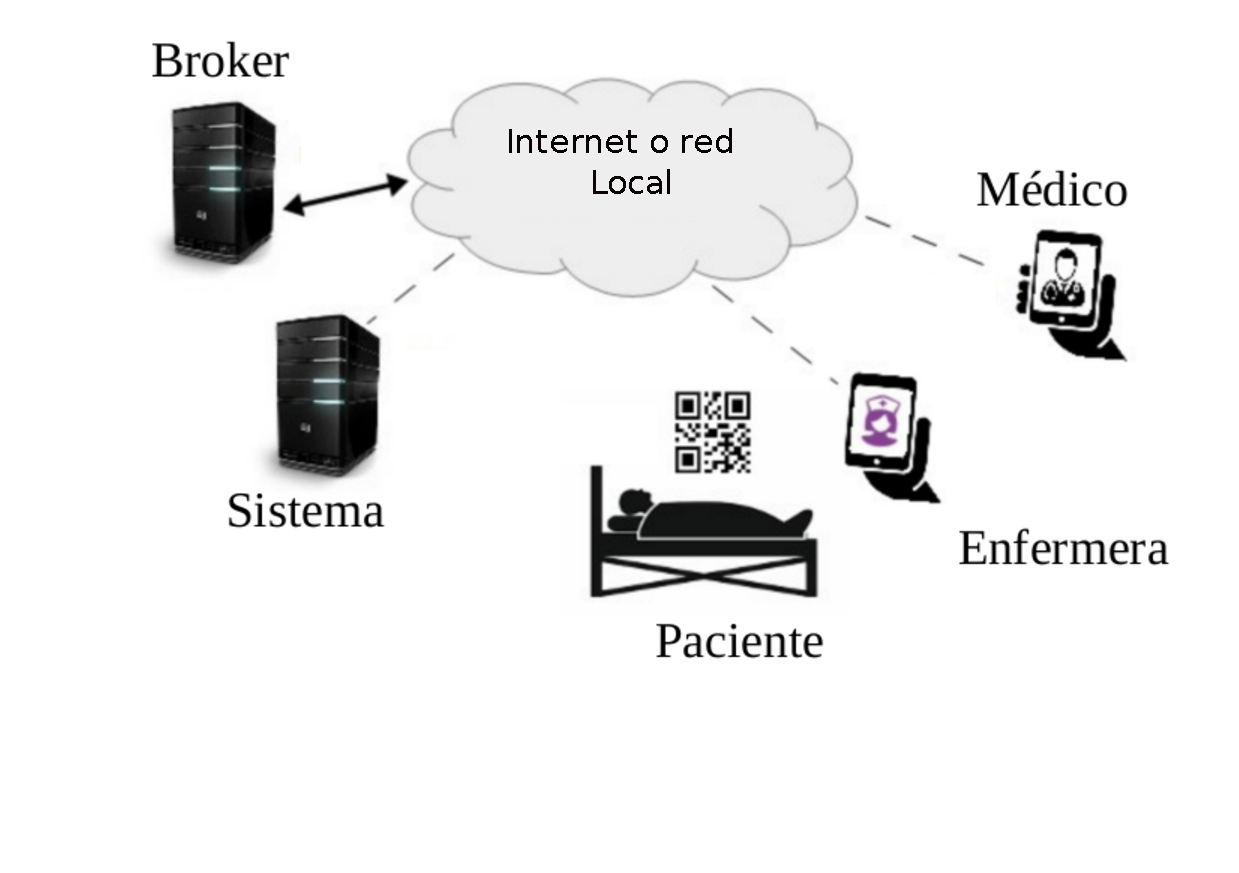
\includegraphics[scale=.45]{./Figures/diag-redux.pdf}
	\caption{Componentes del sistema.}
	\label{fig:Figura-reducida}
\end{figure}


Los componentes del sistema son:
\begin{itemize}
\item broker MQTT: permite gestionar los mensajes entre los elementos del sistema.
\item base de datos: donde alojar información de reportes de habitaciones, personal y datos relevantes al paciente.
\item página web para configuración: permite gestionar usuarios, camas, pacientes, observar estado del sistema.
\item aplicación móvil multiplataforma: permite a los usuarios enfermeros interactuar con el sistema y con los médicos. La aplicación es capaz de identificar la cama correspondiente (mediante lectura de sı́mbolos QR) y de transmitir mensajes de voz en caso de ser necesario.
\end{itemize}


El alcance del trabajo consiste en:
\begin{itemize}
\item Confección de un plan de trabajo.
\item Selección y configuración de un broker MQTT.
\item Desarrollo local de una página web de configuración, que permite asignar medicos a pacientes, asignar tareas programadas a pacientes, asignar códigos QR a camas, asignar tratamientos a pacientes, asignar especialidades a los usuarios enfermeros.
\item Desarrollo local de una aplicación móvil con 3 modos de funcionamiento: modo médico, con envío/recepción de audio/texto/alarmas, modo enfermera con envío/recepción de audio/texto/alarmas y escaneo de QR para identificar paciente, y modo sistema que permite el monitoreo de habitaciones.
\item Código documentación de las aplicaciones realizadas.
\end{itemize}

El presente trabajo no incluye:
\begin{itemize}
\item Manuales de las distintas aplicaciones.
\item Traducciones a distintos idiomas de las aplicaciones.
\item Sistema llamador.
\item Análisis de tráfico en la red.
\item Análisis de seguridad(no se certifica).
\item Contratación de base de datos remota.
\item Contratación e instalación de servidores remotos.
\end{itemize}



%\vspace{1cm}

%\begin{figure}[htbp]
%	\centering
%	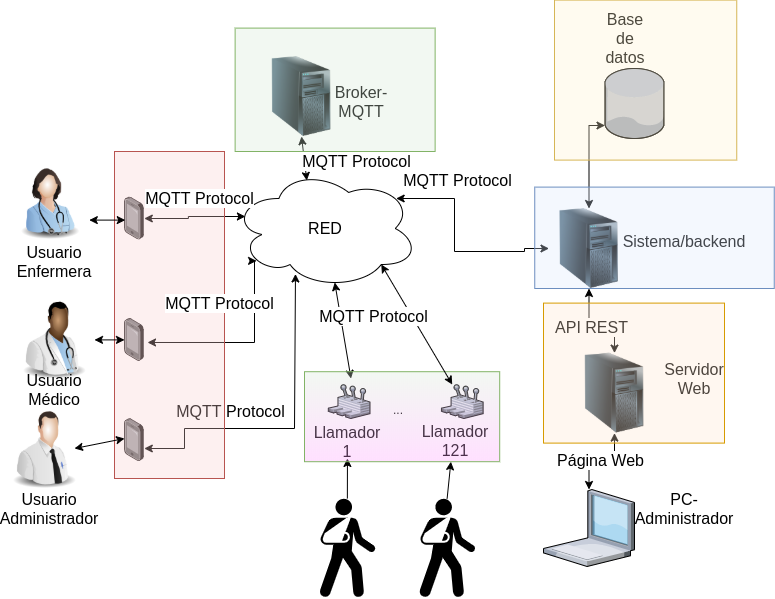
\includegraphics[width=.7\textwidth]{./Figures/DiagramaSistema.png}
%	\caption{Diagrama del Sistema requerido.}
%	\label{fig:texmaker}
%\end{figure}

%\vspace{1cm}


%Si estás escribiendo un documento con mucho contenido matemático, entonces es posible que desees leer el documento de la AMS (American Mathematical Society) llamado, \enquote{A Short Math Guide for \LaTeX{}}. Se puede encontrar en línea en el siguiente link: \url{http://www.ams.org/tex/amslatex.html} en la sección \enquote{Additional Documentation} hacia la parte inferior de la página.


%----------------------------------------------------------------------------------------

%\section{Utilizando esta plantilla}

%Si estás familiarizado con \LaTeX{}, entonces podés explorar la estructura de %directorios de esta plantilla y proceder a personalizarla agregando tu información en el bloque \emph{INFORMACIÓN DE LA PORTADA} en el archivo \file{memoria.tex}.  

%Se puede continuar luego modificando el resto de los archivos siguiendo los lineamientos que se describen en la sección \ref{sec:FillingFile} en la página \pageref{sec:FillingFile}.

%Debés asegurarte de leer el capítulo \ref{Chapter2} acerca de las convenciones utilizadas para las Memoria de los Trabajos Finales de la \degreename.

%Si sos nuevo en \LaTeX{}, se recomienda que continúes leyendo el documento ya que contiene información básica para aprovechar el potencial de esta herramienta.


%----------------------------------------------------------------------------------------

%\section{Qué incluye esta plantilla}

%\subsection{Carpetas}

%Esta plantilla se distribuye como una único archivo .zip que se puede descomprimir en varios archivos y carpetas. Asimismo, se puede consultar el repositorio git para obtener la última versión de los archivos, \url{https://github.com/patriciobos/Plantilla-CESE.git}. Los nombres de las carpetas son, o pretender ser, auto-explicativos.

%\keyword{Appendices} -- Esta es la carpeta donde se deben poner los apéndices. Cada apéndice debe ir en su propio archivo \file{.tex}. Se incluye un ejemplo y una plantilla en la carpeta.

%\keyword{Chapters} -- Esta es la carpeta donde se deben poner los capítulos de la memoria. Cada capítulo debe ir un su propio archivo \file{.tex} por separado.  Se ofrece por defecto, la siguiente estructura de capítulos y se recomienda su utilización dentro de lo posible:

%\begin{itemize}
%\item Capítulo 1: Introducción general	
%\item Capítulo 2: Introducción específica
%\item Capítulo 3: Diseño e implementación
%\item Capítulo 4: Ensayos y resultados
%\item Capítulo 5: Conclusiones

%\end{itemize}

%Esta estructura de capítulos es la que se recomienda para las memorias de la especialización.

%\keyword{Figures} -- Esta carpeta contiene todas las figuras de la memoria.  Estas son las versiones finales de las imágenes que van a ser incluidas en la memoria.  Pueden ser imágenes en formato \textit{raster}\footnote{\url{https://en.wikipedia.org/wiki/Raster_graphics}} como \file{.png}, \file{.jpg} o en formato vectoriales\footnote{\url{https://en.wikipedia.org/wiki/Vector_graphics}} como \file{.pdf}, \file{.ps}.  Se debe notar que utilizar imágenes vectoriales disminuye notablemente el peso del documento final y acelera el tiempo de compilación por lo que es recomendable su utilización siempre que sea posible.

%\subsection{Archivos}

%También están incluidos varios archivos, la mayoría de ellos son de texto plano y se puede ver su contenido en un editor de texto. Después de la compilación inicial, se verá que más archivos auxiliares son creados por \ LaTeX{} o BibTeX, pero son de uso interno y no es necesario hacer nada en particular con ellos.  Toda la información necesaria para compilar el documento se encuentra en los archivos \file{.tex}, \file{.bib}, \file{.cls} y en las imágenes de la carpeta Figures.

%\keyword{referencias.bib} - este es un archivo importante que contiene toda la información de referencias bibliográficas que se utilizarán para las citas en la memoria en conjunto con BibTeX. Usted puede escribir las entradas bibliográficas en forma manual, aunque existen también programas de gestión de referencias que facilitan la creación y gestión de las referencias y permiten exportarlas en formato BibTeX.  También hay disponibles sitios web como \url{books.google.com} que permiten obtener toda la información necesaria para una cita en formato BibTeX. Ver sección \ref{sec:biblio}

%\keyword{MastersDoctoralThesis.cls} -- este es un archivo importante. Es el archivos con la clase que le informa a \LaTeX{} cómo debe dar formato a la memoria. El usuario de la plantilla no debería necesitar modificar nada de este archivo.

%\keyword{memoria.pdf} -- esta es su memoria con una tipografía bellamente compuesta (en formato de archivo PDF) creado por \LaTeX{}. Se distribuye con la plantilla y después de compilar por primera vez sin hacer ningún cambio se debería obtener una versión idéntica a este documento.

%\keyword{memoria.tex} -- este es un archivo importante. Este es el archivo que tiene que compilar \LaTeX{} para producir la memoria como un archivo PDF. Contiene un marco de trabajo y estructuras que le indican a \LaTeX{} cómo diagramar la memoria.  Está altamente comentado para que se pueda entender qué es lo que realiza cada línea de código y por qué está incluida en ese lugar.  En este archivo se debe completar la información personalizada de las primeras sección según se indica en la sección \ref{sec:FillingFile}.

%Archivos que \emph{no} forman parte de la distribución de la plantilla pero que son generados por \LaTeX{} como archivos auxiliares necesarios para la producción de la memoria.pdf son:

%\keyword{memoria.aux} -- este es un archivo auxiliar generado por \LaTeX{}, si se borra \LaTeX{} simplemente lo regenera cuando se compila el archivo principal \file{memoria.tex}.

%\keyword{memoria.bbl} -- este es un archivo auxiliar generado por BibTeX, si se borra BibTeX simplemente lo regenera cuando se compila el archivo principal \file{memoria.tex}. Mientras que el archivo \file{.bib} contiene todas las referencias que hay, este archivo \file{.bbl} contine sólo las referencias que han sido citadas y se utiliza para la construcción de la bibiografía.

%\keyword{memoria.blg} -- este es un archivo auxiliar generado por BibTeX, si se borra BibTeX simplemente lo regenera cuando se compila el archivo principal \file{memoria.tex}.

%\keyword{memoria.lof} -- este es un archivo auxiliar generado por \LaTeX{}, si se borra \LaTeX{} simplemente lo regenera cuando se compila el archivo principal \file{memoria.tex}.  Le indica a \LaTeX{} cómo construir la sección \emph{Lista de Figuras}.
 
%\keyword{memoria.log} --  este es un archivo auxiliar generado por \LaTeX{}, si se borra \LaTeX{} simplemente lo regenera cuando se compila el archivo principal \file{memoria.tex}. Contiene mensajes de \LaTeX{}. Si se reciben errores o advertencias durante la compilación, se guardan en este archivo \file{.log}.

%\keyword{memoria.lot} -- este es un archivo auxiliar generado por \LaTeX{}, si se borra \LaTeX{} simplemente lo regenera cuando se compila el archivo principal \file{memoria.tex}.  Le indica a \LaTeX{} cómo construir la sección \emph{Lista de Tablas}.

%\keyword{memoria.out} -- este es un archivo auxiliar generado por \LaTeX{}, si se borra \LaTeX{} simplemente lo regenera cuando se compila el archivo principal \file{memoria.tex}.

%De esta larga lista de archivos, sólo aquellos con la extensión \file{.bib}, \file{.cls} y \file{.tex} son importantes.  Los otros archivos auxiliares pueden ser ignorados o borrados ya que \LaTeX{} y BibTeX los regenerarán durante la compilación.

%----------------------------------------------------------------------------------------

%\section{Entorno de trabajo}

%Ante de comenzar a editar la plantilla debemos tener un editor \LaTeX{} instalado en nuestra computadora.  En forma análoga a lo que sucede en lenguaje C, que se puede crear y editar código con casi cualquier editor, existen ciertos entornos de trabajo que nos pueden simplificar mucho la tarea.  En este sentido, se recomienda, sobre todo para los principiantes en \LaTeX{} la utilización de TexMaker, un programa gratuito y multi-plantaforma que está disponible tanto para windows como para sistemas GNU/linux.

%La versión más reciente de TexMaker es la 4.5 y se puede descargar del siguiente link: \url{http://www.xm1math.net/texmaker/download.html}. Se puede consultar el manual de usuario en el siguiente link: \url{http://www.xm1math.net/texmaker/doc.html}.
 

%\subsection{Paquetes adicionales}

%Si bien durante el proceso de instalación de TexMaker, o cualquier otro editor que se haya elegido, se instalarán en el sistema los paquetes básicos necesarios para trabajar con \LaTeX{}, la plantilla de los trabajos de Especialización y Maestría requieren de paquete adicionales.

%Se indican a continuación los comandos que se deben introducir en la consola de Ubuntu (ctrl + alt + t) para instalarlos:

%\begin{lstlisting}[language=bash]
%  $ sudo apt install texlive-lang-spanish texlive-science 
%  $ sudo apt install texlive-bibtex-extra biber
%  $ sudo apt install texlive texlive-fonts-recommended
%  $ sudo apt install texlive-latex-extra
%\end{lstlisting}


%\subsection{Configurando TexMaker}



%Una vez instalado el programa y los paquetes adicionales se debe abrir el archivo memoria.tex con el editor para ver una pantalla similar a la que se puede apreciar en la figura \ref{fig:texmaker}. 
%Una vez instalado el programa y los paquetes adicionales se debe abrir el archivo memoria.tex con el editor para ver una pantalla similar a la que se puede apreciar en la figura \ref{fig:texmaker}. 
%Una vez instalado el programa y los paquetes adicionales se debe abrir el archivo memoria.tex con el editor para ver una pantalla similar a la que se puede apreciar en la figura \ref{fig:texmaker}. 
%Una vez instalado el programa y los paquetes adicionales se debe abrir el archivo memoria.tex con el editor para ver una pantalla similar a la que se puede apreciar en la figura \ref{fig:texmaker}. 

%\vspace{1cm}

%\begin{figure}[htbp]
%	\centering
%	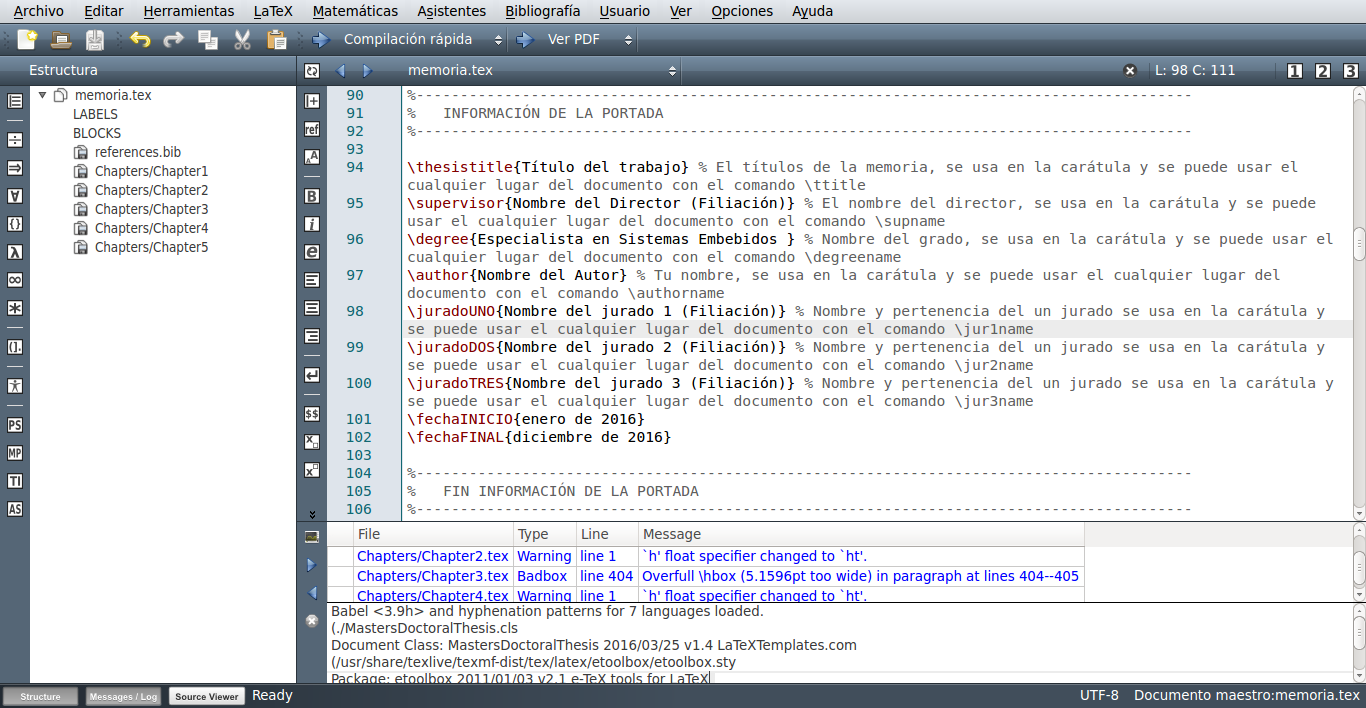
\includegraphics[width=.5\textwidth]{./Figures/texmaker.png}
%	\caption{Entorno de trabajo de texMaker.}
%	\label{fig:texmaker}
%\end{figure}

%\vspace{1cm}

%Notar que existe una vista llamada Estructura a la izquierda de la interfaz que nos permite abrir desde dentro del programa los archivos individuales de los capítulos.  A la derecha se encuentra una vista con el archivo propiamente dicho para su edición. Hacia la parte inferior se encuentra una vista del log con información de los resultados de la compilación.  En esta última vista pueden aparecen advertencias o \textit{warning}, que normalmente pueden ser ignorados, y los errores que se indican en color rojo y deben resolverse para que se genere el PDF de salida.

%Recordar que el archivo que se debe compilar con PDFLaTeX es \file{memoria.tex}, si se tratara de compilar alguno de los capítulos saldría un error.  Para salvar la molestia de tener que cambiar de archivo para compilar cada vez que se realice una modificación en un capítulo, se puede definir el archivo \file{memoria.tex} como ``documento maestro'' yendo al menú opciones -> ``definir documento actual como documento maestro'', lo que permite compilar con PDFLaTeX memoria.tex directamente desde cualquier archivo que se esté modificando . Se muestra esta opción en la figura \ref{fig:docMaestro}.

%\begin{figure}[h]
%	\centering
%	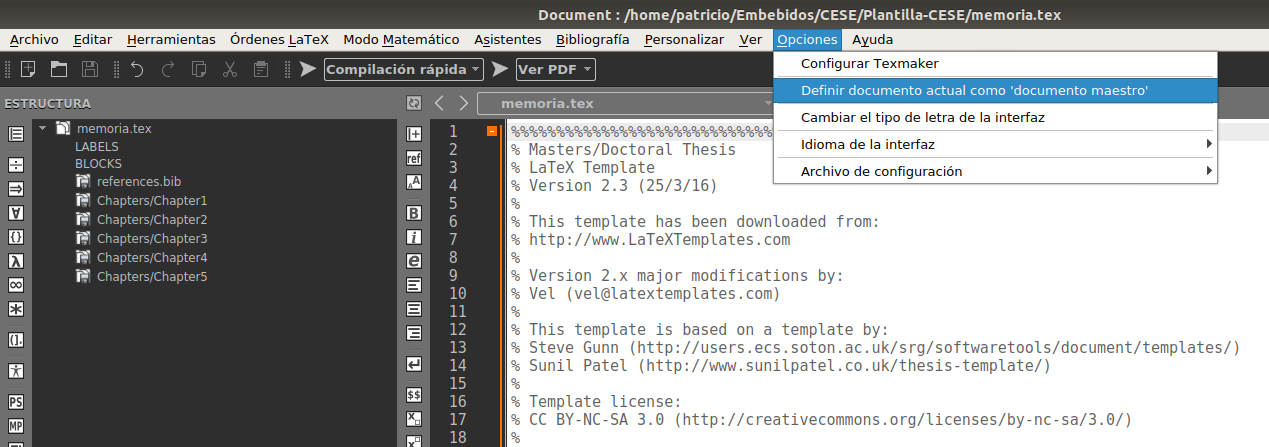
\includegraphics[width=\textwidth]{./Figures/docMaestro.png}
%	\caption{Definir memoria.tex como documento maestro.}
%	\label{fig:docMaestro}
%\end{figure}

%En el menú herramientas se encuentran las opciones de compilación.  Para producir un archivo PDF a partir de un archivo .tex se debe ejecutar PDFLaTeX (el shortcut es F6). Para incorporar nueva bibliografía se debe utilizar la opción BibTeX del mismo menú herramientas (el shortcut es F11).

%Notar que para actualizar las tablas de contenidos se debe ejecutar PDFLaTeX dos veces.  Esto se debe a que es necesario actualizar algunos archivos auxiliares antes de obtener el resultado final.  En forma similar, para actualizar las referencias se debe ejecutar primero PDFLaTeX, después BibTeX y finalmente PDFLaTeX dos veces por idénticos motivos.

%\section{Personalizando la plantilla, el archivo \file{memoria.tex}}
%\label{sec:FillingFile}

%Para personalizar la plantilla se debe incorporar la información propia en los distintos archivos \file{.tex}. 

%Primero abrir \file{memoria.tex} con TexMaker (o el editor de su preferencia). Se debe ubicar dentro del archivo el bloque de código titulado \emph{INFORMACIÓN DE LA PORTADA} donde se deben incorporar los primeros datos personales con los que se construirá automáticamente la portada.


%----------------------------------------------------------------------------------------

%\section{El código del archivo \file{memoria.tex} explicado}

%El archivo \file{memoria.tex} contiene la estructura del documento y es el archivo de mayor jerarquía de la memoria.  Podría ser equiparable a la función \emph{main()} de un programa en C, o mejor dicho al archivo fuente .c donde se encuentra definida la función main().

%La estructura básica de cualquier documento de \LaTeX{} comienza con la definición de clase del documento, es seguida por un preámbulo donde se pueden agregar funcionalidades con el uso de \texttt{paquetes} (equiparables a bibliotecas de C), y finalmente, termina con el cuerpo del documento, donde irá el contenido de la memoria.

%\lstset{%
%  basicstyle=\small\ttfamily,
%  language=[LaTeX]{TeX}
%}

%\begin{lstlisting}
%\documentclass{article}  <- Definicion de clase
%\usepackage{listings}	 <- Preambulo

%\begin{document}	 <- Comienzo del contenido propio 
%	Hello world!
%\end{document}
%\end{lstlisting}


%El archivo \file{memoria.tex} se encuentra densamente comentado para explicar qué páginas, secciones y elementos de formato está creando el código \LaTeX{} en cada línea. El código está dividido en bloques con nombres en mayúsculas para que resulte evidente qué es lo que hace esa porción de código en particular. Inicialmente puede parecer que hay mucho código \LaTeX{}, pero es principalmente código para dar formato a la memoria por lo que no requiere intervención del usuario de la plantilla.  Sí se deben personalizar con su información los bloques indicados como:

%\begin{itemize}
%	\item Informacion de la memoria
%	\item Resumen
%	\item Agradecimientos
%	\item Dedicatoria
%\end{itemize}

%El índice de contenidos, las listas de figura de tablas se generan en forma automática y no requieren intervención ni edición manual por parte del usuario de la plantilla. 

%En la parte final del documento se encuentran los capítulos y los apéndices.  Por defecto se incluyen los 5 capítulos propuestos que se encuentran en la carpeta /Chapters. Cada capítulo se debe escribir en un archivo .tex separado y se debe poner en la carpeta \emph{Chapters} con el nombre \file{Chapter1}, \file{Chapter2}, etc\ldots El código para incluir capítulos desde archivos externos se muestra a continuación.

%\begin{verbatim}
%	% Chapter 1

\chapter{Introducción general} % Main chapter title

\label{Chapter1} % For referencing the chapter elsewhere, use \ref{Chapter1} 
\label{IntroGeneral}
En este capítulo se presentan las necesidades de los sistemas hospitalarios junto con nociones sobre el Internet de las cosas y el protocolo MQTT. Además se mencionan las motivaciones, el estado de arte y el alcance del trabajo.
%----------------------------------------------------------------------------------------

% Define some commands to keep the formatting separated from the content 
\newcommand{\keyword}[1]{\textbf{#1}}
\newcommand{\tabhead}[1]{\textbf{#1}}
\newcommand{\code}[1]{\texttt{#1}}
\newcommand{\file}[1]{\texttt{\bfseries#1}}
\newcommand{\option}[1]{\texttt{\itshape#1}}
\newcommand{\grados}{$^{\circ}$}

%----------------------------------------------------------------------------------------

%\section{Introducción}

%----------------------------------------------------------------------------------------
\section{Internet de las Cosas y las actividades hospitalarias}

En la actualidad, el avance de la Internet de las Cosas (IoT de \textit{Internet of Things} ) y la disminución de costos asociados a la tecnología hacen factible su incorporación a distintos contextos de la vida cotidiana. Un campo de mucho interés es el de infraestructuras hospitalarias inteligentes \citep{ARTICLE:1}.

El término Internet de las Cosas fue utilizado por primera vez en 1990 para describir un sistema cuyos componentes del mundo físico se conectaban a la Internet mediante sensores. En la actualidad se utiliza el término para referirse a escenarios donde la conectividad en red y la capacidad de computo se extiende a objetos, sensores y elementos cotidianos no considerados computadoras, permitiendoles generar, intercambiar y consumir datos con un mínimo de intervención humana \citep{ARTICLE:3}.


Si consideramos a las diferentes personas como un elemento más de un sistema, el ámbito hospitalario cuenta con numerosas entidades que interactuan entre sí como ser: médicos, pacientes, enfermeros, personal de limpieza, personal de seguridad, personal administrativo, dispositivos de iluminación, dispositivos   sonoros, herramientas médicas, puertas, ventanas, ventiladores, acondicionadores de aire, termómetros, etc. Un entorno de estas cualidades es ideal para gestionar con IoT, ya que permite mejorar la calidad del servicio de la salud \citep{ARTICLE:1}.

Un sistema de estas características posee un modelo de capas, presentado en \citep{ARTICLE:4} que separa los conocimientos en cinco categorías con responsabilidades bien definidas: negocio, aplicación, procesamiento, red y percepción. La tabla \ref{tab:Modelo} presenta las funciones reducidas de cada modelo:
\pagebreak

%\begin{verbatim}
\begin{table}[h]
	\centering
	\caption[Modelo de capas IoT]{Modelo de capas sistema IoT.}
	\begin{tabular}{l c c}    
		\toprule
		\textbf{Capa}     & \textbf{Función} \\
		\midrule
		Negocio & Establecer reglas y controlar sistema    \\		
		Aplicación    & Interactuar con el usuario           \\
		Procesamiento  & Almacenar y analizar los datos obtenidos  \\
		Red  & Transportar datos entre dispositivos      \\
		Percepción \citep{ARTICLE:4}  & Realizar mediciones o acciones\\
		\bottomrule
		\hline
	\end{tabular}
	\label{tab:Modelo}
\end{table}
%\end{verbatim}




%\LaTeX{} no es \textsc{WYSIWYG} (What You See is What You Get), a diferencia de los procesadores de texto como Microsoft Word o Pages de Apple o incluso LibreOffice en el mundo open-source. En lugar de ello, un documento escrito para \LaTeX{} es en realidad un archivo de texto simple o llano que \emph{no contiene formato} . Nosotros le decimos a \LaTeX{} cómo deseamos que se aplique el formato en el documento final escribiendo comandos simples entre el texto, por ejemplo, si quiero usar texto en itálicas para dar énfasis, escribo \verb|\it{texto}| y pongo el texto que quiero en itálicas entre medio de las llaves. Esto significa que \LaTeX{} es un lenguaje del tipo \enquote{mark-up}, muy parecido a HTML.


\section{Motivación}

%Si sos nuevo en \LaTeX{}, hay un muy buen libro electrónico - disponible gratuitamente en Internet como un archivo PDF - llamado, \enquote{A (not so short) Introduction to \LaTeX{}}. El título del libro es generalmente acortado a simplemente \emph{lshort}. Puede descargar la versión más reciente en inglés (ya que se actualiza de vez en cuando) desde aquí:
%\url{http://www.ctan.org/tex-archive/info/lshort/english/lshort.pdf}

%Se puede encontrar la versión en español en la lista en esta página: \url{http://www.ctan.org/tex-archive/info/lshort/}
En Argentina muchos hospitales están retrasados en su progreso tecnológico. Por dicha razón, todos los avances en este campo son  necesarios. Por lo explicado en la sección anterior, el gestionar la institución con un sistema de IoT es de suma utilidad.

Surix S.R.L fabrica un sistema IP de llamado a enfermera que está basado en el protocolo SIP. Este consiste en un servidor central y terminales que se encuentran en las habitaciones del hospital. La aplicación principal se ejecuta en una computadora o bien en una tablet y monitorea el estado
de las habitaciones. La principal motivación para migrar el protocolo radica en el alto costo de hardware que genera el agregar dispositivos a su sistema actual. En este contexto, se encargó la realización de este trabajo.



\section{Estado de arte}

En el mercado internacional se encontró un producto similar  desarrollado por la firma TigerConnect (antes llamada TigerText), \textit{TigerConnect Clinical Collaboration Platform}(Plataforma de Colaboración Clínica TigerConnect) \citep{WEBSITE:2}, cuyas principales características se detallan a continuación:
\begin{itemize}
\item Aplicación de Mensajería para celulares y estaciones de trabajo.
\item Solución en la nube asegurando disponibilidad en un 99.99\%.
\item Mensajería por texto asegurada con encriptación.  
\item Homologado por HIPPA(del ingles, \textit{Health Insurance Portability and Accountability Act},ley de Portabilidad y Responsabilidad del Seguro Médico)  \citep{WEBSITE:3}.  
\item Certificado HITRUST(es un framework para gestionar riesgos utilizado por muchas redes de salud y hospitales \citep{WEBSITE:1}).  
\item Control administrativo total, permitiendo a los administradores gestionar usuarios, configuraciones y políticas de seguridad por medio de una consola. Los usuarios pueden ser cargados utilizando plantillas csv, y en caso de robo o extravío de dispositivo, prohibir el acceso.  
\item Posibilidad de incorporar mensajería de voz como servicio extra.  
\item Mensajes a grupos de personas.  
\end{itemize}

Entre las diferencias que posee la solución presentada en este trabajo con respecto a la disponible en el mercado se encuentra el hecho de utilizar MQTT como protocolo base permite incorporar con muy poco esfuerzo dispositivos IoT de mediciones paramétricas de los pacientes ya que la estructura de la red asi lo permite. Por otra parte, la solución desarrollada presenta de base la posibilidad de transmisión de audio. 



\section{Objetivos y alcance}

El sistema resultante de este trabajo está orientado a gestionar las relaciones entre pacientes, enfermeras y médicos. Un diagrama reducido puede observarse en la figura \ref{fig:Figura-reducida}.  
%La forma correcta de utilizar una figura es con referencias cruzadas, por ejemplo: ``Se eligió utilizar un cuadrado azul para el logo, como puede observarse en la figura \ref{fig:cuadradoAzul}''.

\begin{figure}[ht]
	\centering
	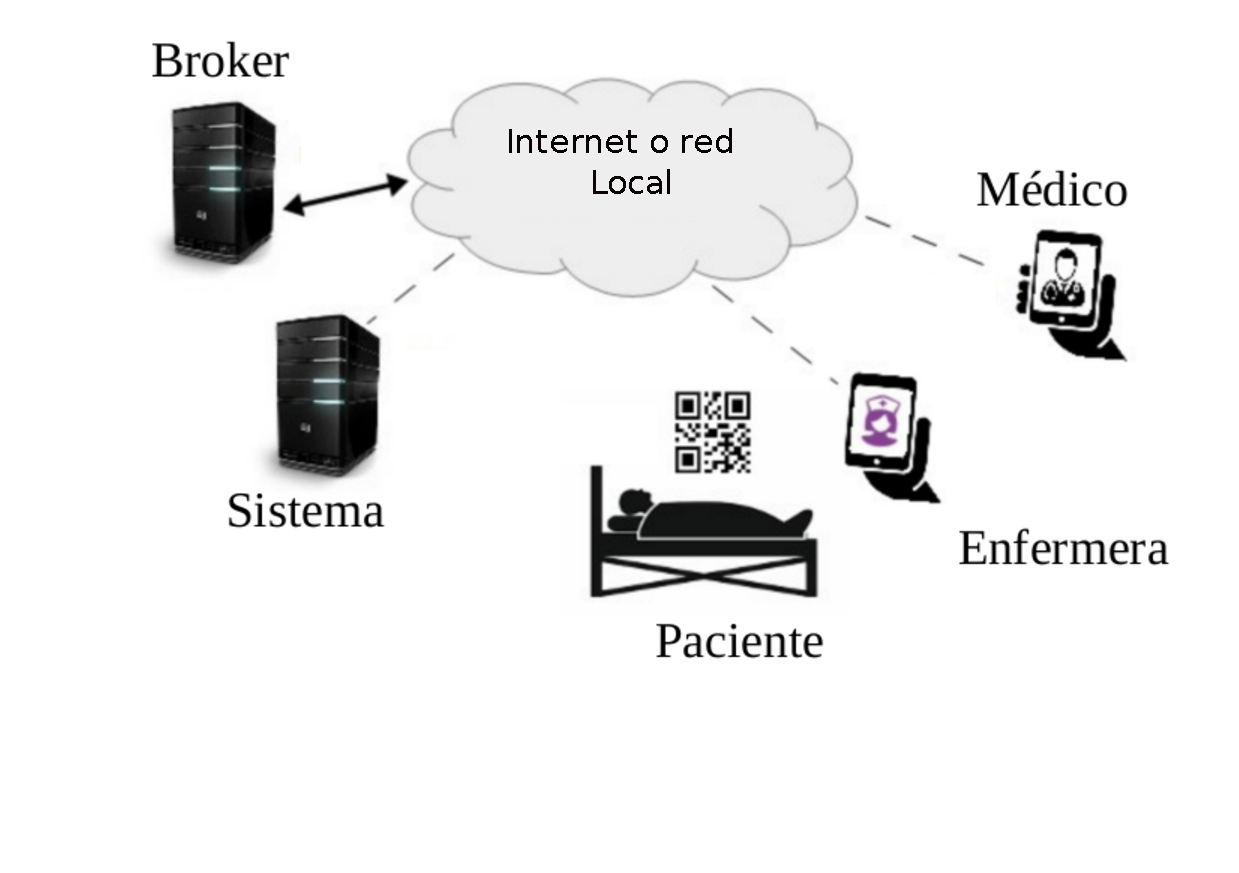
\includegraphics[scale=.45]{./Figures/diag-redux.pdf}
	\caption{Componentes del sistema.}
	\label{fig:Figura-reducida}
\end{figure}


Los componentes del sistema son:
\begin{itemize}
\item broker MQTT: permite gestionar los mensajes entre los elementos del sistema.
\item base de datos: donde alojar información de reportes de habitaciones, personal y datos relevantes al paciente.
\item página web para configuración: permite gestionar usuarios, camas, pacientes, observar estado del sistema.
\item aplicación móvil multiplataforma: permite a los usuarios enfermeros interactuar con el sistema y con los médicos. La aplicación es capaz de identificar la cama correspondiente (mediante lectura de sı́mbolos QR) y de transmitir mensajes de voz en caso de ser necesario.
\end{itemize}


El alcance del trabajo consiste en:
\begin{itemize}
\item Confección de un plan de trabajo.
\item Selección y configuración de un broker MQTT.
\item Desarrollo local de una página web de configuración, que permite asignar medicos a pacientes, asignar tareas programadas a pacientes, asignar códigos QR a camas, asignar tratamientos a pacientes, asignar especialidades a los usuarios enfermeros.
\item Desarrollo local de una aplicación móvil con 3 modos de funcionamiento: modo médico, con envío/recepción de audio/texto/alarmas, modo enfermera con envío/recepción de audio/texto/alarmas y escaneo de QR para identificar paciente, y modo sistema que permite el monitoreo de habitaciones.
\item Código documentación de las aplicaciones realizadas.
\end{itemize}

El presente trabajo no incluye:
\begin{itemize}
\item Manuales de las distintas aplicaciones.
\item Traducciones a distintos idiomas de las aplicaciones.
\item Sistema llamador.
\item Análisis de tráfico en la red.
\item Análisis de seguridad(no se certifica).
\item Contratación de base de datos remota.
\item Contratación e instalación de servidores remotos.
\end{itemize}



%\vspace{1cm}

%\begin{figure}[htbp]
%	\centering
%	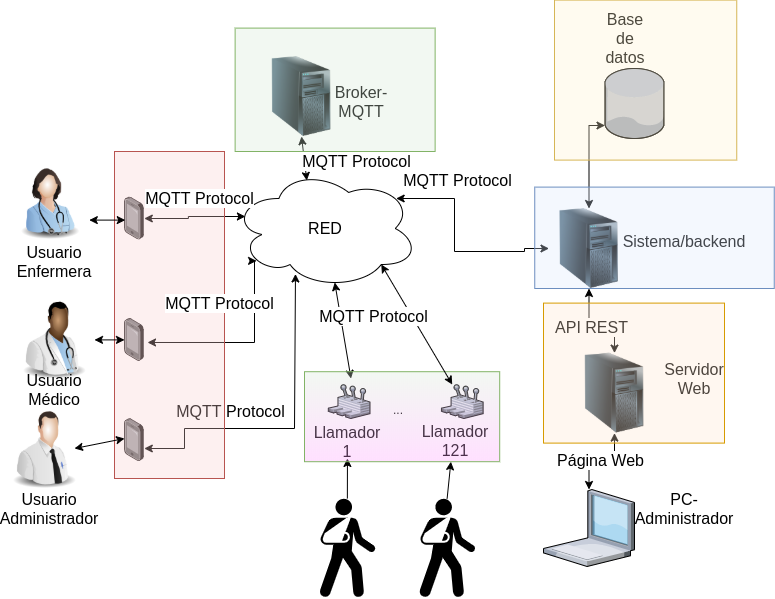
\includegraphics[width=.7\textwidth]{./Figures/DiagramaSistema.png}
%	\caption{Diagrama del Sistema requerido.}
%	\label{fig:texmaker}
%\end{figure}

%\vspace{1cm}


%Si estás escribiendo un documento con mucho contenido matemático, entonces es posible que desees leer el documento de la AMS (American Mathematical Society) llamado, \enquote{A Short Math Guide for \LaTeX{}}. Se puede encontrar en línea en el siguiente link: \url{http://www.ams.org/tex/amslatex.html} en la sección \enquote{Additional Documentation} hacia la parte inferior de la página.


%----------------------------------------------------------------------------------------

%\section{Utilizando esta plantilla}

%Si estás familiarizado con \LaTeX{}, entonces podés explorar la estructura de %directorios de esta plantilla y proceder a personalizarla agregando tu información en el bloque \emph{INFORMACIÓN DE LA PORTADA} en el archivo \file{memoria.tex}.  

%Se puede continuar luego modificando el resto de los archivos siguiendo los lineamientos que se describen en la sección \ref{sec:FillingFile} en la página \pageref{sec:FillingFile}.

%Debés asegurarte de leer el capítulo \ref{Chapter2} acerca de las convenciones utilizadas para las Memoria de los Trabajos Finales de la \degreename.

%Si sos nuevo en \LaTeX{}, se recomienda que continúes leyendo el documento ya que contiene información básica para aprovechar el potencial de esta herramienta.


%----------------------------------------------------------------------------------------

%\section{Qué incluye esta plantilla}

%\subsection{Carpetas}

%Esta plantilla se distribuye como una único archivo .zip que se puede descomprimir en varios archivos y carpetas. Asimismo, se puede consultar el repositorio git para obtener la última versión de los archivos, \url{https://github.com/patriciobos/Plantilla-CESE.git}. Los nombres de las carpetas son, o pretender ser, auto-explicativos.

%\keyword{Appendices} -- Esta es la carpeta donde se deben poner los apéndices. Cada apéndice debe ir en su propio archivo \file{.tex}. Se incluye un ejemplo y una plantilla en la carpeta.

%\keyword{Chapters} -- Esta es la carpeta donde se deben poner los capítulos de la memoria. Cada capítulo debe ir un su propio archivo \file{.tex} por separado.  Se ofrece por defecto, la siguiente estructura de capítulos y se recomienda su utilización dentro de lo posible:

%\begin{itemize}
%\item Capítulo 1: Introducción general	
%\item Capítulo 2: Introducción específica
%\item Capítulo 3: Diseño e implementación
%\item Capítulo 4: Ensayos y resultados
%\item Capítulo 5: Conclusiones

%\end{itemize}

%Esta estructura de capítulos es la que se recomienda para las memorias de la especialización.

%\keyword{Figures} -- Esta carpeta contiene todas las figuras de la memoria.  Estas son las versiones finales de las imágenes que van a ser incluidas en la memoria.  Pueden ser imágenes en formato \textit{raster}\footnote{\url{https://en.wikipedia.org/wiki/Raster_graphics}} como \file{.png}, \file{.jpg} o en formato vectoriales\footnote{\url{https://en.wikipedia.org/wiki/Vector_graphics}} como \file{.pdf}, \file{.ps}.  Se debe notar que utilizar imágenes vectoriales disminuye notablemente el peso del documento final y acelera el tiempo de compilación por lo que es recomendable su utilización siempre que sea posible.

%\subsection{Archivos}

%También están incluidos varios archivos, la mayoría de ellos son de texto plano y se puede ver su contenido en un editor de texto. Después de la compilación inicial, se verá que más archivos auxiliares son creados por \ LaTeX{} o BibTeX, pero son de uso interno y no es necesario hacer nada en particular con ellos.  Toda la información necesaria para compilar el documento se encuentra en los archivos \file{.tex}, \file{.bib}, \file{.cls} y en las imágenes de la carpeta Figures.

%\keyword{referencias.bib} - este es un archivo importante que contiene toda la información de referencias bibliográficas que se utilizarán para las citas en la memoria en conjunto con BibTeX. Usted puede escribir las entradas bibliográficas en forma manual, aunque existen también programas de gestión de referencias que facilitan la creación y gestión de las referencias y permiten exportarlas en formato BibTeX.  También hay disponibles sitios web como \url{books.google.com} que permiten obtener toda la información necesaria para una cita en formato BibTeX. Ver sección \ref{sec:biblio}

%\keyword{MastersDoctoralThesis.cls} -- este es un archivo importante. Es el archivos con la clase que le informa a \LaTeX{} cómo debe dar formato a la memoria. El usuario de la plantilla no debería necesitar modificar nada de este archivo.

%\keyword{memoria.pdf} -- esta es su memoria con una tipografía bellamente compuesta (en formato de archivo PDF) creado por \LaTeX{}. Se distribuye con la plantilla y después de compilar por primera vez sin hacer ningún cambio se debería obtener una versión idéntica a este documento.

%\keyword{memoria.tex} -- este es un archivo importante. Este es el archivo que tiene que compilar \LaTeX{} para producir la memoria como un archivo PDF. Contiene un marco de trabajo y estructuras que le indican a \LaTeX{} cómo diagramar la memoria.  Está altamente comentado para que se pueda entender qué es lo que realiza cada línea de código y por qué está incluida en ese lugar.  En este archivo se debe completar la información personalizada de las primeras sección según se indica en la sección \ref{sec:FillingFile}.

%Archivos que \emph{no} forman parte de la distribución de la plantilla pero que son generados por \LaTeX{} como archivos auxiliares necesarios para la producción de la memoria.pdf son:

%\keyword{memoria.aux} -- este es un archivo auxiliar generado por \LaTeX{}, si se borra \LaTeX{} simplemente lo regenera cuando se compila el archivo principal \file{memoria.tex}.

%\keyword{memoria.bbl} -- este es un archivo auxiliar generado por BibTeX, si se borra BibTeX simplemente lo regenera cuando se compila el archivo principal \file{memoria.tex}. Mientras que el archivo \file{.bib} contiene todas las referencias que hay, este archivo \file{.bbl} contine sólo las referencias que han sido citadas y se utiliza para la construcción de la bibiografía.

%\keyword{memoria.blg} -- este es un archivo auxiliar generado por BibTeX, si se borra BibTeX simplemente lo regenera cuando se compila el archivo principal \file{memoria.tex}.

%\keyword{memoria.lof} -- este es un archivo auxiliar generado por \LaTeX{}, si se borra \LaTeX{} simplemente lo regenera cuando se compila el archivo principal \file{memoria.tex}.  Le indica a \LaTeX{} cómo construir la sección \emph{Lista de Figuras}.
 
%\keyword{memoria.log} --  este es un archivo auxiliar generado por \LaTeX{}, si se borra \LaTeX{} simplemente lo regenera cuando se compila el archivo principal \file{memoria.tex}. Contiene mensajes de \LaTeX{}. Si se reciben errores o advertencias durante la compilación, se guardan en este archivo \file{.log}.

%\keyword{memoria.lot} -- este es un archivo auxiliar generado por \LaTeX{}, si se borra \LaTeX{} simplemente lo regenera cuando se compila el archivo principal \file{memoria.tex}.  Le indica a \LaTeX{} cómo construir la sección \emph{Lista de Tablas}.

%\keyword{memoria.out} -- este es un archivo auxiliar generado por \LaTeX{}, si se borra \LaTeX{} simplemente lo regenera cuando se compila el archivo principal \file{memoria.tex}.

%De esta larga lista de archivos, sólo aquellos con la extensión \file{.bib}, \file{.cls} y \file{.tex} son importantes.  Los otros archivos auxiliares pueden ser ignorados o borrados ya que \LaTeX{} y BibTeX los regenerarán durante la compilación.

%----------------------------------------------------------------------------------------

%\section{Entorno de trabajo}

%Ante de comenzar a editar la plantilla debemos tener un editor \LaTeX{} instalado en nuestra computadora.  En forma análoga a lo que sucede en lenguaje C, que se puede crear y editar código con casi cualquier editor, existen ciertos entornos de trabajo que nos pueden simplificar mucho la tarea.  En este sentido, se recomienda, sobre todo para los principiantes en \LaTeX{} la utilización de TexMaker, un programa gratuito y multi-plantaforma que está disponible tanto para windows como para sistemas GNU/linux.

%La versión más reciente de TexMaker es la 4.5 y se puede descargar del siguiente link: \url{http://www.xm1math.net/texmaker/download.html}. Se puede consultar el manual de usuario en el siguiente link: \url{http://www.xm1math.net/texmaker/doc.html}.
 

%\subsection{Paquetes adicionales}

%Si bien durante el proceso de instalación de TexMaker, o cualquier otro editor que se haya elegido, se instalarán en el sistema los paquetes básicos necesarios para trabajar con \LaTeX{}, la plantilla de los trabajos de Especialización y Maestría requieren de paquete adicionales.

%Se indican a continuación los comandos que se deben introducir en la consola de Ubuntu (ctrl + alt + t) para instalarlos:

%\begin{lstlisting}[language=bash]
%  $ sudo apt install texlive-lang-spanish texlive-science 
%  $ sudo apt install texlive-bibtex-extra biber
%  $ sudo apt install texlive texlive-fonts-recommended
%  $ sudo apt install texlive-latex-extra
%\end{lstlisting}


%\subsection{Configurando TexMaker}



%Una vez instalado el programa y los paquetes adicionales se debe abrir el archivo memoria.tex con el editor para ver una pantalla similar a la que se puede apreciar en la figura \ref{fig:texmaker}. 
%Una vez instalado el programa y los paquetes adicionales se debe abrir el archivo memoria.tex con el editor para ver una pantalla similar a la que se puede apreciar en la figura \ref{fig:texmaker}. 
%Una vez instalado el programa y los paquetes adicionales se debe abrir el archivo memoria.tex con el editor para ver una pantalla similar a la que se puede apreciar en la figura \ref{fig:texmaker}. 
%Una vez instalado el programa y los paquetes adicionales se debe abrir el archivo memoria.tex con el editor para ver una pantalla similar a la que se puede apreciar en la figura \ref{fig:texmaker}. 

%\vspace{1cm}

%\begin{figure}[htbp]
%	\centering
%	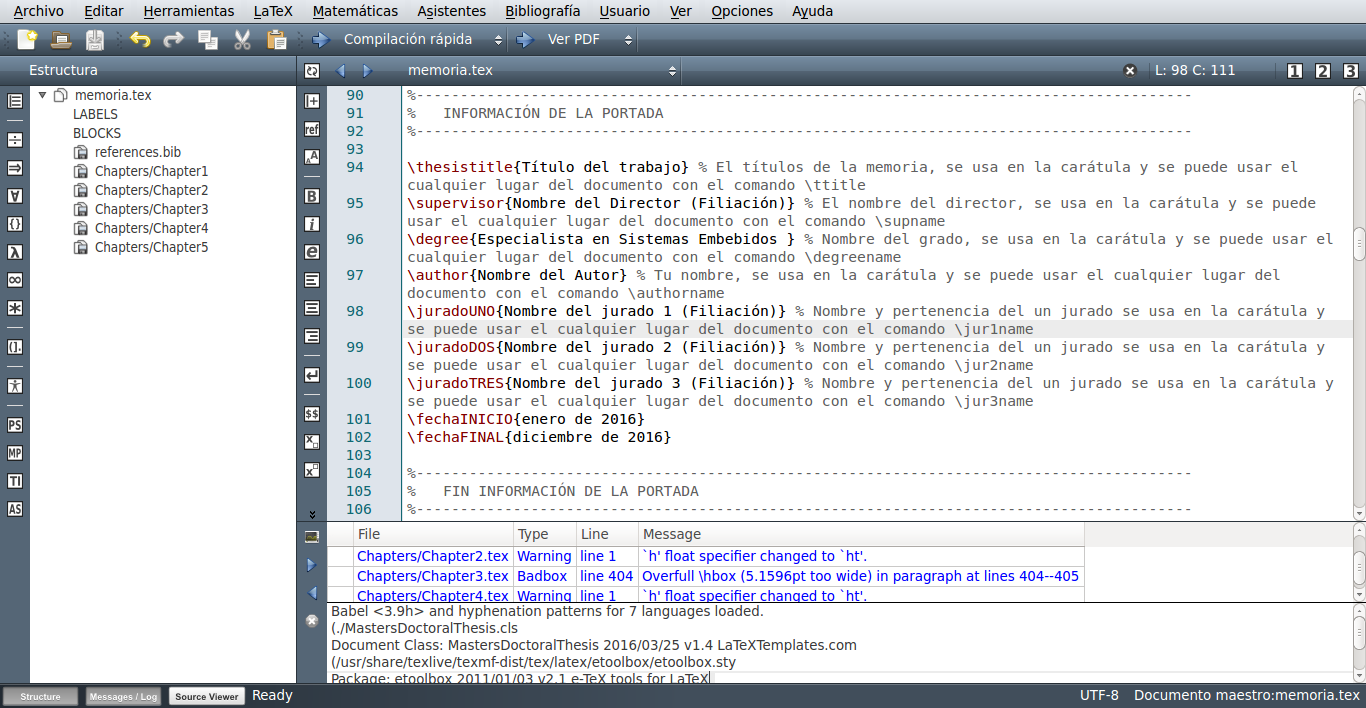
\includegraphics[width=.5\textwidth]{./Figures/texmaker.png}
%	\caption{Entorno de trabajo de texMaker.}
%	\label{fig:texmaker}
%\end{figure}

%\vspace{1cm}

%Notar que existe una vista llamada Estructura a la izquierda de la interfaz que nos permite abrir desde dentro del programa los archivos individuales de los capítulos.  A la derecha se encuentra una vista con el archivo propiamente dicho para su edición. Hacia la parte inferior se encuentra una vista del log con información de los resultados de la compilación.  En esta última vista pueden aparecen advertencias o \textit{warning}, que normalmente pueden ser ignorados, y los errores que se indican en color rojo y deben resolverse para que se genere el PDF de salida.

%Recordar que el archivo que se debe compilar con PDFLaTeX es \file{memoria.tex}, si se tratara de compilar alguno de los capítulos saldría un error.  Para salvar la molestia de tener que cambiar de archivo para compilar cada vez que se realice una modificación en un capítulo, se puede definir el archivo \file{memoria.tex} como ``documento maestro'' yendo al menú opciones -> ``definir documento actual como documento maestro'', lo que permite compilar con PDFLaTeX memoria.tex directamente desde cualquier archivo que se esté modificando . Se muestra esta opción en la figura \ref{fig:docMaestro}.

%\begin{figure}[h]
%	\centering
%	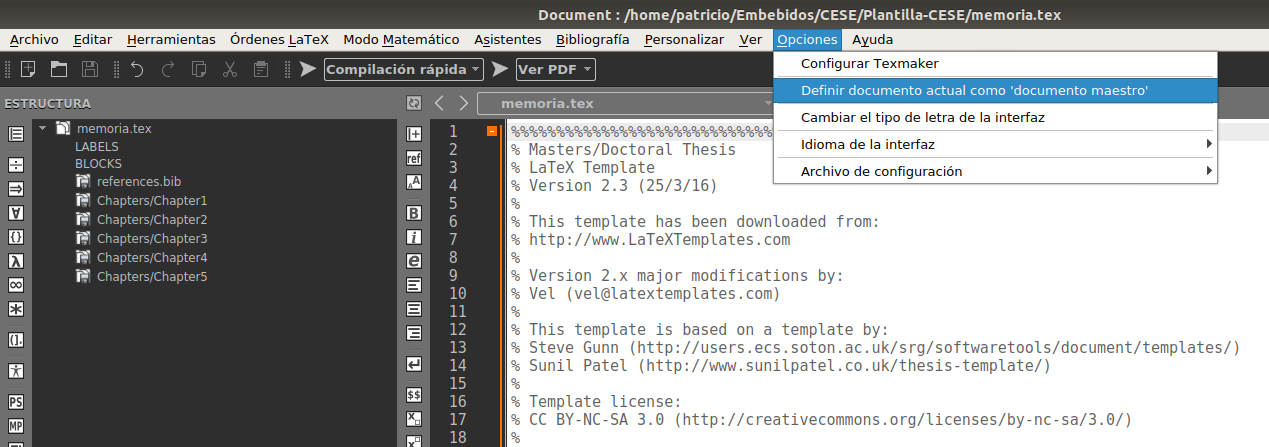
\includegraphics[width=\textwidth]{./Figures/docMaestro.png}
%	\caption{Definir memoria.tex como documento maestro.}
%	\label{fig:docMaestro}
%\end{figure}

%En el menú herramientas se encuentran las opciones de compilación.  Para producir un archivo PDF a partir de un archivo .tex se debe ejecutar PDFLaTeX (el shortcut es F6). Para incorporar nueva bibliografía se debe utilizar la opción BibTeX del mismo menú herramientas (el shortcut es F11).

%Notar que para actualizar las tablas de contenidos se debe ejecutar PDFLaTeX dos veces.  Esto se debe a que es necesario actualizar algunos archivos auxiliares antes de obtener el resultado final.  En forma similar, para actualizar las referencias se debe ejecutar primero PDFLaTeX, después BibTeX y finalmente PDFLaTeX dos veces por idénticos motivos.

%\section{Personalizando la plantilla, el archivo \file{memoria.tex}}
%\label{sec:FillingFile}

%Para personalizar la plantilla se debe incorporar la información propia en los distintos archivos \file{.tex}. 

%Primero abrir \file{memoria.tex} con TexMaker (o el editor de su preferencia). Se debe ubicar dentro del archivo el bloque de código titulado \emph{INFORMACIÓN DE LA PORTADA} donde se deben incorporar los primeros datos personales con los que se construirá automáticamente la portada.


%----------------------------------------------------------------------------------------

%\section{El código del archivo \file{memoria.tex} explicado}

%El archivo \file{memoria.tex} contiene la estructura del documento y es el archivo de mayor jerarquía de la memoria.  Podría ser equiparable a la función \emph{main()} de un programa en C, o mejor dicho al archivo fuente .c donde se encuentra definida la función main().

%La estructura básica de cualquier documento de \LaTeX{} comienza con la definición de clase del documento, es seguida por un preámbulo donde se pueden agregar funcionalidades con el uso de \texttt{paquetes} (equiparables a bibliotecas de C), y finalmente, termina con el cuerpo del documento, donde irá el contenido de la memoria.

%\lstset{%
%  basicstyle=\small\ttfamily,
%  language=[LaTeX]{TeX}
%}

%\begin{lstlisting}
%\documentclass{article}  <- Definicion de clase
%\usepackage{listings}	 <- Preambulo

%\begin{document}	 <- Comienzo del contenido propio 
%	Hello world!
%\end{document}
%\end{lstlisting}


%El archivo \file{memoria.tex} se encuentra densamente comentado para explicar qué páginas, secciones y elementos de formato está creando el código \LaTeX{} en cada línea. El código está dividido en bloques con nombres en mayúsculas para que resulte evidente qué es lo que hace esa porción de código en particular. Inicialmente puede parecer que hay mucho código \LaTeX{}, pero es principalmente código para dar formato a la memoria por lo que no requiere intervención del usuario de la plantilla.  Sí se deben personalizar con su información los bloques indicados como:

%\begin{itemize}
%	\item Informacion de la memoria
%	\item Resumen
%	\item Agradecimientos
%	\item Dedicatoria
%\end{itemize}

%El índice de contenidos, las listas de figura de tablas se generan en forma automática y no requieren intervención ni edición manual por parte del usuario de la plantilla. 

%En la parte final del documento se encuentran los capítulos y los apéndices.  Por defecto se incluyen los 5 capítulos propuestos que se encuentran en la carpeta /Chapters. Cada capítulo se debe escribir en un archivo .tex separado y se debe poner en la carpeta \emph{Chapters} con el nombre \file{Chapter1}, \file{Chapter2}, etc\ldots El código para incluir capítulos desde archivos externos se muestra a continuación.

%\begin{verbatim}
%	% Chapter 1

\chapter{Introducción general} % Main chapter title

\label{Chapter1} % For referencing the chapter elsewhere, use \ref{Chapter1} 
\label{IntroGeneral}
En este capítulo se presentan las necesidades de los sistemas hospitalarios junto con nociones sobre el Internet de las cosas y el protocolo MQTT. Además se mencionan las motivaciones, el estado de arte y el alcance del trabajo.
%----------------------------------------------------------------------------------------

% Define some commands to keep the formatting separated from the content 
\newcommand{\keyword}[1]{\textbf{#1}}
\newcommand{\tabhead}[1]{\textbf{#1}}
\newcommand{\code}[1]{\texttt{#1}}
\newcommand{\file}[1]{\texttt{\bfseries#1}}
\newcommand{\option}[1]{\texttt{\itshape#1}}
\newcommand{\grados}{$^{\circ}$}

%----------------------------------------------------------------------------------------

%\section{Introducción}

%----------------------------------------------------------------------------------------
\section{Internet de las Cosas y las actividades hospitalarias}

En la actualidad, el avance de la Internet de las Cosas (IoT de \textit{Internet of Things} ) y la disminución de costos asociados a la tecnología hacen factible su incorporación a distintos contextos de la vida cotidiana. Un campo de mucho interés es el de infraestructuras hospitalarias inteligentes \citep{ARTICLE:1}.

El término Internet de las Cosas fue utilizado por primera vez en 1990 para describir un sistema cuyos componentes del mundo físico se conectaban a la Internet mediante sensores. En la actualidad se utiliza el término para referirse a escenarios donde la conectividad en red y la capacidad de computo se extiende a objetos, sensores y elementos cotidianos no considerados computadoras, permitiendoles generar, intercambiar y consumir datos con un mínimo de intervención humana \citep{ARTICLE:3}.


Si consideramos a las diferentes personas como un elemento más de un sistema, el ámbito hospitalario cuenta con numerosas entidades que interactuan entre sí como ser: médicos, pacientes, enfermeros, personal de limpieza, personal de seguridad, personal administrativo, dispositivos de iluminación, dispositivos   sonoros, herramientas médicas, puertas, ventanas, ventiladores, acondicionadores de aire, termómetros, etc. Un entorno de estas cualidades es ideal para gestionar con IoT, ya que permite mejorar la calidad del servicio de la salud \citep{ARTICLE:1}.

Un sistema de estas características posee un modelo de capas, presentado en \citep{ARTICLE:4} que separa los conocimientos en cinco categorías con responsabilidades bien definidas: negocio, aplicación, procesamiento, red y percepción. La tabla \ref{tab:Modelo} presenta las funciones reducidas de cada modelo:
\pagebreak

%\begin{verbatim}
\begin{table}[h]
	\centering
	\caption[Modelo de capas IoT]{Modelo de capas sistema IoT.}
	\begin{tabular}{l c c}    
		\toprule
		\textbf{Capa}     & \textbf{Función} \\
		\midrule
		Negocio & Establecer reglas y controlar sistema    \\		
		Aplicación    & Interactuar con el usuario           \\
		Procesamiento  & Almacenar y analizar los datos obtenidos  \\
		Red  & Transportar datos entre dispositivos      \\
		Percepción \citep{ARTICLE:4}  & Realizar mediciones o acciones\\
		\bottomrule
		\hline
	\end{tabular}
	\label{tab:Modelo}
\end{table}
%\end{verbatim}




%\LaTeX{} no es \textsc{WYSIWYG} (What You See is What You Get), a diferencia de los procesadores de texto como Microsoft Word o Pages de Apple o incluso LibreOffice en el mundo open-source. En lugar de ello, un documento escrito para \LaTeX{} es en realidad un archivo de texto simple o llano que \emph{no contiene formato} . Nosotros le decimos a \LaTeX{} cómo deseamos que se aplique el formato en el documento final escribiendo comandos simples entre el texto, por ejemplo, si quiero usar texto en itálicas para dar énfasis, escribo \verb|\it{texto}| y pongo el texto que quiero en itálicas entre medio de las llaves. Esto significa que \LaTeX{} es un lenguaje del tipo \enquote{mark-up}, muy parecido a HTML.


\section{Motivación}

%Si sos nuevo en \LaTeX{}, hay un muy buen libro electrónico - disponible gratuitamente en Internet como un archivo PDF - llamado, \enquote{A (not so short) Introduction to \LaTeX{}}. El título del libro es generalmente acortado a simplemente \emph{lshort}. Puede descargar la versión más reciente en inglés (ya que se actualiza de vez en cuando) desde aquí:
%\url{http://www.ctan.org/tex-archive/info/lshort/english/lshort.pdf}

%Se puede encontrar la versión en español en la lista en esta página: \url{http://www.ctan.org/tex-archive/info/lshort/}
En Argentina muchos hospitales están retrasados en su progreso tecnológico. Por dicha razón, todos los avances en este campo son  necesarios. Por lo explicado en la sección anterior, el gestionar la institución con un sistema de IoT es de suma utilidad.

Surix S.R.L fabrica un sistema IP de llamado a enfermera que está basado en el protocolo SIP. Este consiste en un servidor central y terminales que se encuentran en las habitaciones del hospital. La aplicación principal se ejecuta en una computadora o bien en una tablet y monitorea el estado
de las habitaciones. La principal motivación para migrar el protocolo radica en el alto costo de hardware que genera el agregar dispositivos a su sistema actual. En este contexto, se encargó la realización de este trabajo.



\section{Estado de arte}

En el mercado internacional se encontró un producto similar  desarrollado por la firma TigerConnect (antes llamada TigerText), \textit{TigerConnect Clinical Collaboration Platform}(Plataforma de Colaboración Clínica TigerConnect) \citep{WEBSITE:2}, cuyas principales características se detallan a continuación:
\begin{itemize}
\item Aplicación de Mensajería para celulares y estaciones de trabajo.
\item Solución en la nube asegurando disponibilidad en un 99.99\%.
\item Mensajería por texto asegurada con encriptación.  
\item Homologado por HIPPA(del ingles, \textit{Health Insurance Portability and Accountability Act},ley de Portabilidad y Responsabilidad del Seguro Médico)  \citep{WEBSITE:3}.  
\item Certificado HITRUST(es un framework para gestionar riesgos utilizado por muchas redes de salud y hospitales \citep{WEBSITE:1}).  
\item Control administrativo total, permitiendo a los administradores gestionar usuarios, configuraciones y políticas de seguridad por medio de una consola. Los usuarios pueden ser cargados utilizando plantillas csv, y en caso de robo o extravío de dispositivo, prohibir el acceso.  
\item Posibilidad de incorporar mensajería de voz como servicio extra.  
\item Mensajes a grupos de personas.  
\end{itemize}

Entre las diferencias que posee la solución presentada en este trabajo con respecto a la disponible en el mercado se encuentra el hecho de utilizar MQTT como protocolo base permite incorporar con muy poco esfuerzo dispositivos IoT de mediciones paramétricas de los pacientes ya que la estructura de la red asi lo permite. Por otra parte, la solución desarrollada presenta de base la posibilidad de transmisión de audio. 



\section{Objetivos y alcance}

El sistema resultante de este trabajo está orientado a gestionar las relaciones entre pacientes, enfermeras y médicos. Un diagrama reducido puede observarse en la figura \ref{fig:Figura-reducida}.  
%La forma correcta de utilizar una figura es con referencias cruzadas, por ejemplo: ``Se eligió utilizar un cuadrado azul para el logo, como puede observarse en la figura \ref{fig:cuadradoAzul}''.

\begin{figure}[ht]
	\centering
	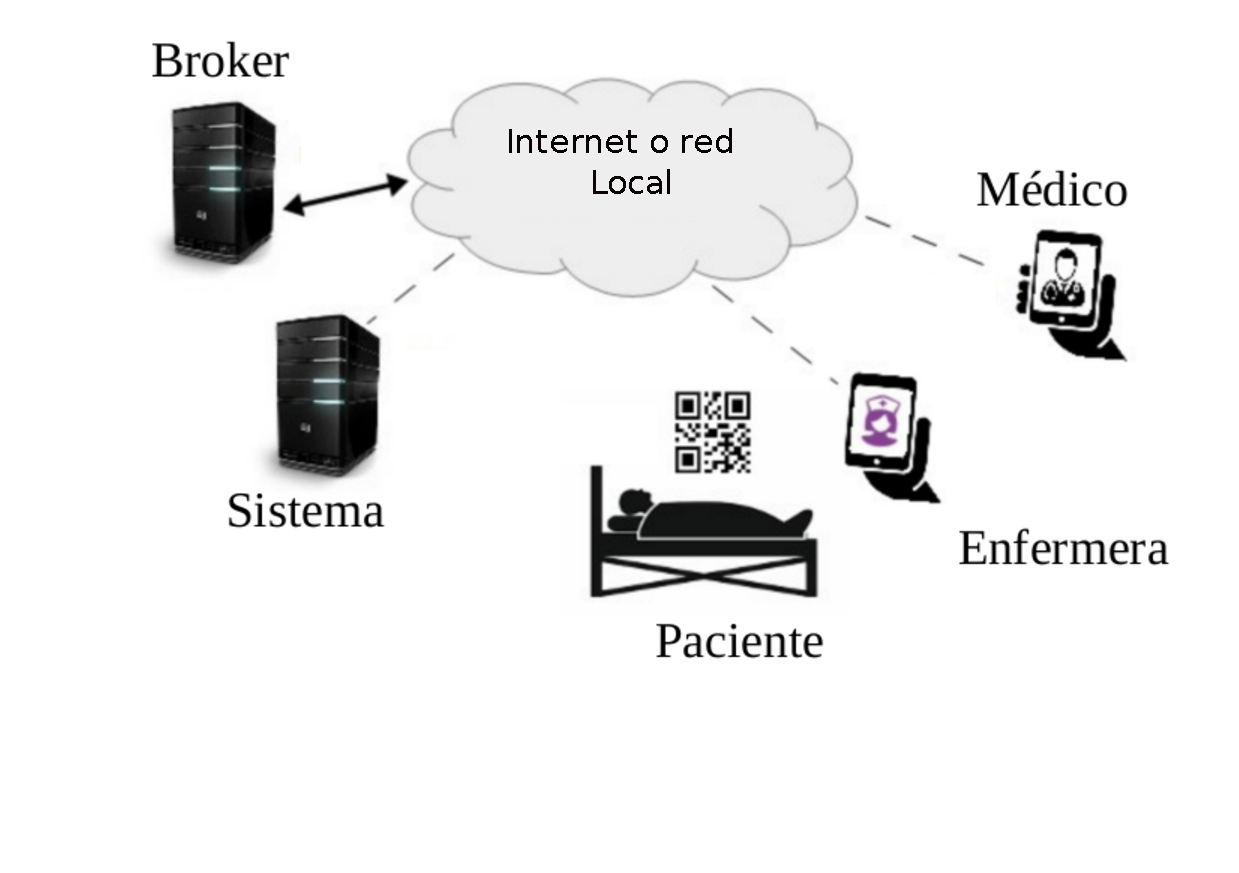
\includegraphics[scale=.45]{./Figures/diag-redux.pdf}
	\caption{Componentes del sistema.}
	\label{fig:Figura-reducida}
\end{figure}


Los componentes del sistema son:
\begin{itemize}
\item broker MQTT: permite gestionar los mensajes entre los elementos del sistema.
\item base de datos: donde alojar información de reportes de habitaciones, personal y datos relevantes al paciente.
\item página web para configuración: permite gestionar usuarios, camas, pacientes, observar estado del sistema.
\item aplicación móvil multiplataforma: permite a los usuarios enfermeros interactuar con el sistema y con los médicos. La aplicación es capaz de identificar la cama correspondiente (mediante lectura de sı́mbolos QR) y de transmitir mensajes de voz en caso de ser necesario.
\end{itemize}


El alcance del trabajo consiste en:
\begin{itemize}
\item Confección de un plan de trabajo.
\item Selección y configuración de un broker MQTT.
\item Desarrollo local de una página web de configuración, que permite asignar medicos a pacientes, asignar tareas programadas a pacientes, asignar códigos QR a camas, asignar tratamientos a pacientes, asignar especialidades a los usuarios enfermeros.
\item Desarrollo local de una aplicación móvil con 3 modos de funcionamiento: modo médico, con envío/recepción de audio/texto/alarmas, modo enfermera con envío/recepción de audio/texto/alarmas y escaneo de QR para identificar paciente, y modo sistema que permite el monitoreo de habitaciones.
\item Código documentación de las aplicaciones realizadas.
\end{itemize}

El presente trabajo no incluye:
\begin{itemize}
\item Manuales de las distintas aplicaciones.
\item Traducciones a distintos idiomas de las aplicaciones.
\item Sistema llamador.
\item Análisis de tráfico en la red.
\item Análisis de seguridad(no se certifica).
\item Contratación de base de datos remota.
\item Contratación e instalación de servidores remotos.
\end{itemize}



%\vspace{1cm}

%\begin{figure}[htbp]
%	\centering
%	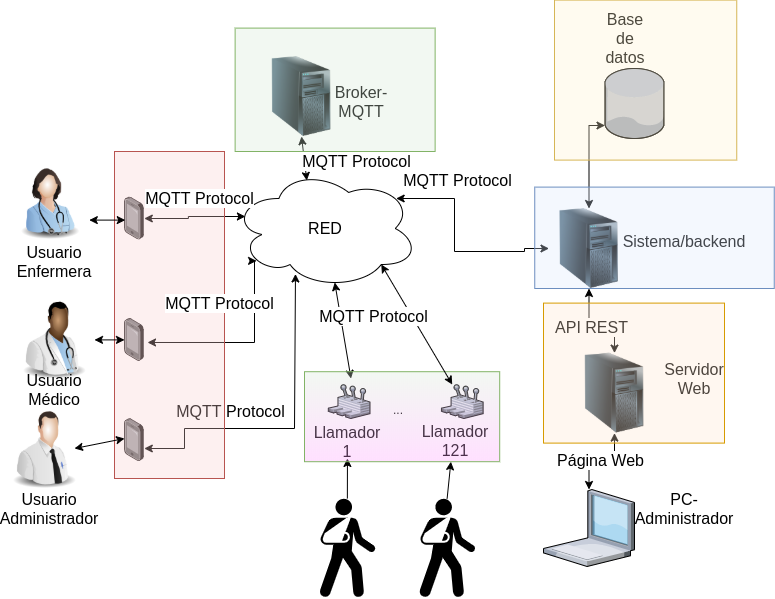
\includegraphics[width=.7\textwidth]{./Figures/DiagramaSistema.png}
%	\caption{Diagrama del Sistema requerido.}
%	\label{fig:texmaker}
%\end{figure}

%\vspace{1cm}


%Si estás escribiendo un documento con mucho contenido matemático, entonces es posible que desees leer el documento de la AMS (American Mathematical Society) llamado, \enquote{A Short Math Guide for \LaTeX{}}. Se puede encontrar en línea en el siguiente link: \url{http://www.ams.org/tex/amslatex.html} en la sección \enquote{Additional Documentation} hacia la parte inferior de la página.


%----------------------------------------------------------------------------------------

%\section{Utilizando esta plantilla}

%Si estás familiarizado con \LaTeX{}, entonces podés explorar la estructura de %directorios de esta plantilla y proceder a personalizarla agregando tu información en el bloque \emph{INFORMACIÓN DE LA PORTADA} en el archivo \file{memoria.tex}.  

%Se puede continuar luego modificando el resto de los archivos siguiendo los lineamientos que se describen en la sección \ref{sec:FillingFile} en la página \pageref{sec:FillingFile}.

%Debés asegurarte de leer el capítulo \ref{Chapter2} acerca de las convenciones utilizadas para las Memoria de los Trabajos Finales de la \degreename.

%Si sos nuevo en \LaTeX{}, se recomienda que continúes leyendo el documento ya que contiene información básica para aprovechar el potencial de esta herramienta.


%----------------------------------------------------------------------------------------

%\section{Qué incluye esta plantilla}

%\subsection{Carpetas}

%Esta plantilla se distribuye como una único archivo .zip que se puede descomprimir en varios archivos y carpetas. Asimismo, se puede consultar el repositorio git para obtener la última versión de los archivos, \url{https://github.com/patriciobos/Plantilla-CESE.git}. Los nombres de las carpetas son, o pretender ser, auto-explicativos.

%\keyword{Appendices} -- Esta es la carpeta donde se deben poner los apéndices. Cada apéndice debe ir en su propio archivo \file{.tex}. Se incluye un ejemplo y una plantilla en la carpeta.

%\keyword{Chapters} -- Esta es la carpeta donde se deben poner los capítulos de la memoria. Cada capítulo debe ir un su propio archivo \file{.tex} por separado.  Se ofrece por defecto, la siguiente estructura de capítulos y se recomienda su utilización dentro de lo posible:

%\begin{itemize}
%\item Capítulo 1: Introducción general	
%\item Capítulo 2: Introducción específica
%\item Capítulo 3: Diseño e implementación
%\item Capítulo 4: Ensayos y resultados
%\item Capítulo 5: Conclusiones

%\end{itemize}

%Esta estructura de capítulos es la que se recomienda para las memorias de la especialización.

%\keyword{Figures} -- Esta carpeta contiene todas las figuras de la memoria.  Estas son las versiones finales de las imágenes que van a ser incluidas en la memoria.  Pueden ser imágenes en formato \textit{raster}\footnote{\url{https://en.wikipedia.org/wiki/Raster_graphics}} como \file{.png}, \file{.jpg} o en formato vectoriales\footnote{\url{https://en.wikipedia.org/wiki/Vector_graphics}} como \file{.pdf}, \file{.ps}.  Se debe notar que utilizar imágenes vectoriales disminuye notablemente el peso del documento final y acelera el tiempo de compilación por lo que es recomendable su utilización siempre que sea posible.

%\subsection{Archivos}

%También están incluidos varios archivos, la mayoría de ellos son de texto plano y se puede ver su contenido en un editor de texto. Después de la compilación inicial, se verá que más archivos auxiliares son creados por \ LaTeX{} o BibTeX, pero son de uso interno y no es necesario hacer nada en particular con ellos.  Toda la información necesaria para compilar el documento se encuentra en los archivos \file{.tex}, \file{.bib}, \file{.cls} y en las imágenes de la carpeta Figures.

%\keyword{referencias.bib} - este es un archivo importante que contiene toda la información de referencias bibliográficas que se utilizarán para las citas en la memoria en conjunto con BibTeX. Usted puede escribir las entradas bibliográficas en forma manual, aunque existen también programas de gestión de referencias que facilitan la creación y gestión de las referencias y permiten exportarlas en formato BibTeX.  También hay disponibles sitios web como \url{books.google.com} que permiten obtener toda la información necesaria para una cita en formato BibTeX. Ver sección \ref{sec:biblio}

%\keyword{MastersDoctoralThesis.cls} -- este es un archivo importante. Es el archivos con la clase que le informa a \LaTeX{} cómo debe dar formato a la memoria. El usuario de la plantilla no debería necesitar modificar nada de este archivo.

%\keyword{memoria.pdf} -- esta es su memoria con una tipografía bellamente compuesta (en formato de archivo PDF) creado por \LaTeX{}. Se distribuye con la plantilla y después de compilar por primera vez sin hacer ningún cambio se debería obtener una versión idéntica a este documento.

%\keyword{memoria.tex} -- este es un archivo importante. Este es el archivo que tiene que compilar \LaTeX{} para producir la memoria como un archivo PDF. Contiene un marco de trabajo y estructuras que le indican a \LaTeX{} cómo diagramar la memoria.  Está altamente comentado para que se pueda entender qué es lo que realiza cada línea de código y por qué está incluida en ese lugar.  En este archivo se debe completar la información personalizada de las primeras sección según se indica en la sección \ref{sec:FillingFile}.

%Archivos que \emph{no} forman parte de la distribución de la plantilla pero que son generados por \LaTeX{} como archivos auxiliares necesarios para la producción de la memoria.pdf son:

%\keyword{memoria.aux} -- este es un archivo auxiliar generado por \LaTeX{}, si se borra \LaTeX{} simplemente lo regenera cuando se compila el archivo principal \file{memoria.tex}.

%\keyword{memoria.bbl} -- este es un archivo auxiliar generado por BibTeX, si se borra BibTeX simplemente lo regenera cuando se compila el archivo principal \file{memoria.tex}. Mientras que el archivo \file{.bib} contiene todas las referencias que hay, este archivo \file{.bbl} contine sólo las referencias que han sido citadas y se utiliza para la construcción de la bibiografía.

%\keyword{memoria.blg} -- este es un archivo auxiliar generado por BibTeX, si se borra BibTeX simplemente lo regenera cuando se compila el archivo principal \file{memoria.tex}.

%\keyword{memoria.lof} -- este es un archivo auxiliar generado por \LaTeX{}, si se borra \LaTeX{} simplemente lo regenera cuando se compila el archivo principal \file{memoria.tex}.  Le indica a \LaTeX{} cómo construir la sección \emph{Lista de Figuras}.
 
%\keyword{memoria.log} --  este es un archivo auxiliar generado por \LaTeX{}, si se borra \LaTeX{} simplemente lo regenera cuando se compila el archivo principal \file{memoria.tex}. Contiene mensajes de \LaTeX{}. Si se reciben errores o advertencias durante la compilación, se guardan en este archivo \file{.log}.

%\keyword{memoria.lot} -- este es un archivo auxiliar generado por \LaTeX{}, si se borra \LaTeX{} simplemente lo regenera cuando se compila el archivo principal \file{memoria.tex}.  Le indica a \LaTeX{} cómo construir la sección \emph{Lista de Tablas}.

%\keyword{memoria.out} -- este es un archivo auxiliar generado por \LaTeX{}, si se borra \LaTeX{} simplemente lo regenera cuando se compila el archivo principal \file{memoria.tex}.

%De esta larga lista de archivos, sólo aquellos con la extensión \file{.bib}, \file{.cls} y \file{.tex} son importantes.  Los otros archivos auxiliares pueden ser ignorados o borrados ya que \LaTeX{} y BibTeX los regenerarán durante la compilación.

%----------------------------------------------------------------------------------------

%\section{Entorno de trabajo}

%Ante de comenzar a editar la plantilla debemos tener un editor \LaTeX{} instalado en nuestra computadora.  En forma análoga a lo que sucede en lenguaje C, que se puede crear y editar código con casi cualquier editor, existen ciertos entornos de trabajo que nos pueden simplificar mucho la tarea.  En este sentido, se recomienda, sobre todo para los principiantes en \LaTeX{} la utilización de TexMaker, un programa gratuito y multi-plantaforma que está disponible tanto para windows como para sistemas GNU/linux.

%La versión más reciente de TexMaker es la 4.5 y se puede descargar del siguiente link: \url{http://www.xm1math.net/texmaker/download.html}. Se puede consultar el manual de usuario en el siguiente link: \url{http://www.xm1math.net/texmaker/doc.html}.
 

%\subsection{Paquetes adicionales}

%Si bien durante el proceso de instalación de TexMaker, o cualquier otro editor que se haya elegido, se instalarán en el sistema los paquetes básicos necesarios para trabajar con \LaTeX{}, la plantilla de los trabajos de Especialización y Maestría requieren de paquete adicionales.

%Se indican a continuación los comandos que se deben introducir en la consola de Ubuntu (ctrl + alt + t) para instalarlos:

%\begin{lstlisting}[language=bash]
%  $ sudo apt install texlive-lang-spanish texlive-science 
%  $ sudo apt install texlive-bibtex-extra biber
%  $ sudo apt install texlive texlive-fonts-recommended
%  $ sudo apt install texlive-latex-extra
%\end{lstlisting}


%\subsection{Configurando TexMaker}



%Una vez instalado el programa y los paquetes adicionales se debe abrir el archivo memoria.tex con el editor para ver una pantalla similar a la que se puede apreciar en la figura \ref{fig:texmaker}. 
%Una vez instalado el programa y los paquetes adicionales se debe abrir el archivo memoria.tex con el editor para ver una pantalla similar a la que se puede apreciar en la figura \ref{fig:texmaker}. 
%Una vez instalado el programa y los paquetes adicionales se debe abrir el archivo memoria.tex con el editor para ver una pantalla similar a la que se puede apreciar en la figura \ref{fig:texmaker}. 
%Una vez instalado el programa y los paquetes adicionales se debe abrir el archivo memoria.tex con el editor para ver una pantalla similar a la que se puede apreciar en la figura \ref{fig:texmaker}. 

%\vspace{1cm}

%\begin{figure}[htbp]
%	\centering
%	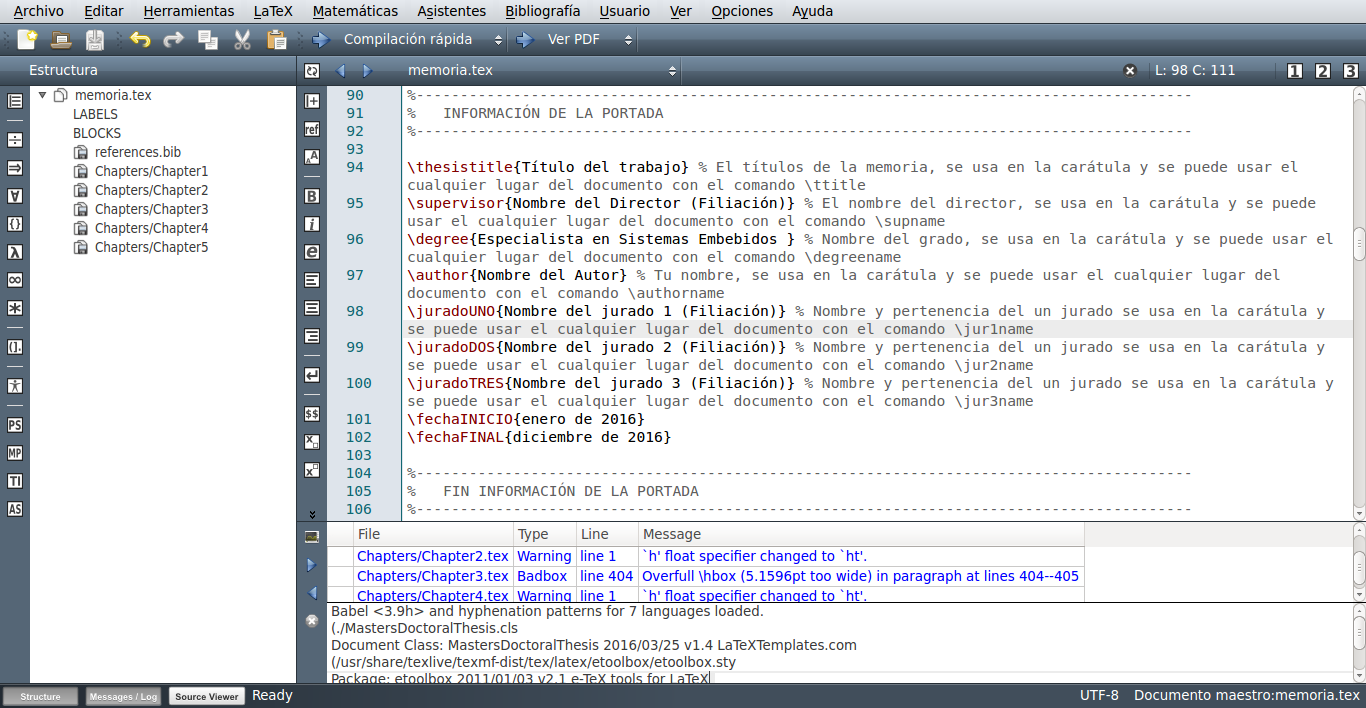
\includegraphics[width=.5\textwidth]{./Figures/texmaker.png}
%	\caption{Entorno de trabajo de texMaker.}
%	\label{fig:texmaker}
%\end{figure}

%\vspace{1cm}

%Notar que existe una vista llamada Estructura a la izquierda de la interfaz que nos permite abrir desde dentro del programa los archivos individuales de los capítulos.  A la derecha se encuentra una vista con el archivo propiamente dicho para su edición. Hacia la parte inferior se encuentra una vista del log con información de los resultados de la compilación.  En esta última vista pueden aparecen advertencias o \textit{warning}, que normalmente pueden ser ignorados, y los errores que se indican en color rojo y deben resolverse para que se genere el PDF de salida.

%Recordar que el archivo que se debe compilar con PDFLaTeX es \file{memoria.tex}, si se tratara de compilar alguno de los capítulos saldría un error.  Para salvar la molestia de tener que cambiar de archivo para compilar cada vez que se realice una modificación en un capítulo, se puede definir el archivo \file{memoria.tex} como ``documento maestro'' yendo al menú opciones -> ``definir documento actual como documento maestro'', lo que permite compilar con PDFLaTeX memoria.tex directamente desde cualquier archivo que se esté modificando . Se muestra esta opción en la figura \ref{fig:docMaestro}.

%\begin{figure}[h]
%	\centering
%	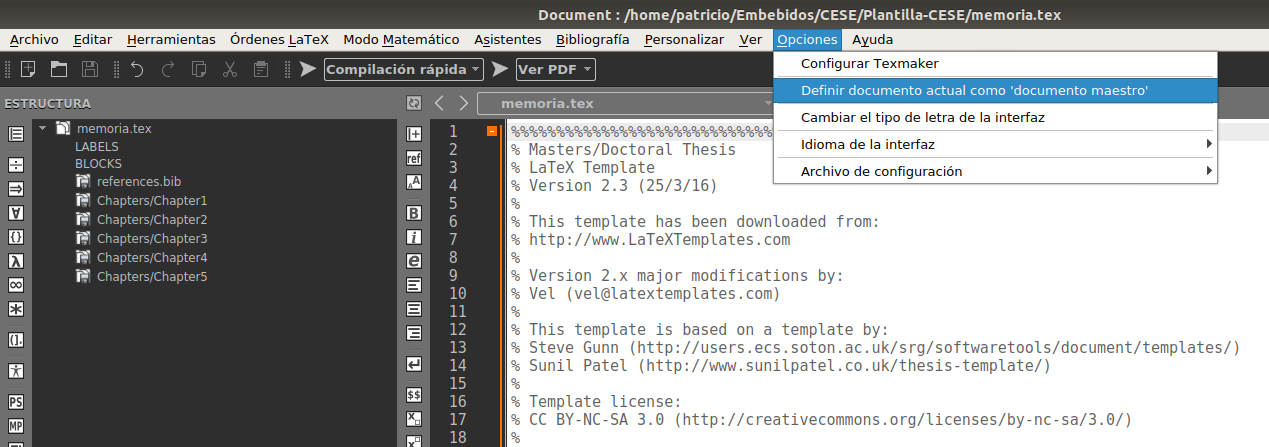
\includegraphics[width=\textwidth]{./Figures/docMaestro.png}
%	\caption{Definir memoria.tex como documento maestro.}
%	\label{fig:docMaestro}
%\end{figure}

%En el menú herramientas se encuentran las opciones de compilación.  Para producir un archivo PDF a partir de un archivo .tex se debe ejecutar PDFLaTeX (el shortcut es F6). Para incorporar nueva bibliografía se debe utilizar la opción BibTeX del mismo menú herramientas (el shortcut es F11).

%Notar que para actualizar las tablas de contenidos se debe ejecutar PDFLaTeX dos veces.  Esto se debe a que es necesario actualizar algunos archivos auxiliares antes de obtener el resultado final.  En forma similar, para actualizar las referencias se debe ejecutar primero PDFLaTeX, después BibTeX y finalmente PDFLaTeX dos veces por idénticos motivos.

%\section{Personalizando la plantilla, el archivo \file{memoria.tex}}
%\label{sec:FillingFile}

%Para personalizar la plantilla se debe incorporar la información propia en los distintos archivos \file{.tex}. 

%Primero abrir \file{memoria.tex} con TexMaker (o el editor de su preferencia). Se debe ubicar dentro del archivo el bloque de código titulado \emph{INFORMACIÓN DE LA PORTADA} donde se deben incorporar los primeros datos personales con los que se construirá automáticamente la portada.


%----------------------------------------------------------------------------------------

%\section{El código del archivo \file{memoria.tex} explicado}

%El archivo \file{memoria.tex} contiene la estructura del documento y es el archivo de mayor jerarquía de la memoria.  Podría ser equiparable a la función \emph{main()} de un programa en C, o mejor dicho al archivo fuente .c donde se encuentra definida la función main().

%La estructura básica de cualquier documento de \LaTeX{} comienza con la definición de clase del documento, es seguida por un preámbulo donde se pueden agregar funcionalidades con el uso de \texttt{paquetes} (equiparables a bibliotecas de C), y finalmente, termina con el cuerpo del documento, donde irá el contenido de la memoria.

%\lstset{%
%  basicstyle=\small\ttfamily,
%  language=[LaTeX]{TeX}
%}

%\begin{lstlisting}
%\documentclass{article}  <- Definicion de clase
%\usepackage{listings}	 <- Preambulo

%\begin{document}	 <- Comienzo del contenido propio 
%	Hello world!
%\end{document}
%\end{lstlisting}


%El archivo \file{memoria.tex} se encuentra densamente comentado para explicar qué páginas, secciones y elementos de formato está creando el código \LaTeX{} en cada línea. El código está dividido en bloques con nombres en mayúsculas para que resulte evidente qué es lo que hace esa porción de código en particular. Inicialmente puede parecer que hay mucho código \LaTeX{}, pero es principalmente código para dar formato a la memoria por lo que no requiere intervención del usuario de la plantilla.  Sí se deben personalizar con su información los bloques indicados como:

%\begin{itemize}
%	\item Informacion de la memoria
%	\item Resumen
%	\item Agradecimientos
%	\item Dedicatoria
%\end{itemize}

%El índice de contenidos, las listas de figura de tablas se generan en forma automática y no requieren intervención ni edición manual por parte del usuario de la plantilla. 

%En la parte final del documento se encuentran los capítulos y los apéndices.  Por defecto se incluyen los 5 capítulos propuestos que se encuentran en la carpeta /Chapters. Cada capítulo se debe escribir en un archivo .tex separado y se debe poner en la carpeta \emph{Chapters} con el nombre \file{Chapter1}, \file{Chapter2}, etc\ldots El código para incluir capítulos desde archivos externos se muestra a continuación.

%\begin{verbatim}
%	\include{Chapters/Chapter1}
%	\include{Chapters/Chapter2} 
%	\include{Chapters/Chapter3}
%	\include{Chapters/Chapter4} 
%	\include{Chapters/Chapter5} 
%\end{verbatim}

%Los apéndices también deben escribirse en archivos .tex separados, que se deben ubicar dentro de la carpeta \emph{Appendices}. Los apéndices vienen comentados por defecto con el caracter \code{\%} y para incluirlos simplemente se debe eliminar dicho caracter.

%Finalmente, se encuentra el código para incluir la bibliografía en el documento final.  Este código tampoco debe modificarse. La metodología para trabajar las referencias bibliográficas se desarrolla en la sección \ref{sec:biblio}.
%----------------------------------------------------------------------------------------

%\section{Bibliografía}
%\label{sec:biblio}

%Las opciones de formato de la bibliografía se controlan a través del paquete de latex \option{biblatex} que se incluye en la memoria en el archivo memoria.tex.  Estas opciones determinan cómo se generan las citas bibliográficas en el cuerpo del documento y cómo se genera la bibliografía al final de la memoria.

%En el preámbulo se puede encontrar el código que incluye el paquete biblatex, que no requiere ninguna modificación del usuario de la plantilla, y que contiene las siguientes opciones:

%\begin{lstlisting}
%\usepackage[backend=bibtex,
%	natbib=true, 
%	style=numeric, 
%	sorting=none]
%{biblatex}
%\end{lstlisting}

%En el archivo \file{reference.bib} se encuentran las referencias bibliográficas que se pueden citar en el documento.  Para incorporar una nueva cita al documento lo primero es agregarla en este archivo con todos los campos necesario.  Todas las entradas bibliográficas comienzan con $@$ y una palabra que define el formato de la entrada.  Para cada formato existen campos obligatorios que deben completarse. No importa el orden en que las entradas estén definidas en el archivo .bib.  Tampoco es importante el orden en que estén definidos los campos de una entrada bibliográfica. A continuación se muestran algunos ejemplos:

%\begin{lstlisting}
%@ARTICLE{ARTICLE:1,
%    AUTHOR="John Doe",
%    TITLE="Title",
%    JOURNAL="Journal",
%    YEAR="2017",
%}
%\end{lstlisting}


%\begin{lstlisting}
%@BOOK{BOOK:1,
%    AUTHOR="John Doe",
%    TITLE="The Book without Title",
%    PUBLISHER="Dummy Publisher",
%    YEAR="2100",
%}
%\end{lstlisting}


%\begin{lstlisting}
%@INBOOK{BOOK:2,
%    AUTHOR="John Doe",
%    TITLE="The Book without Title",
%    PUBLISHER="Dummy Publisher",
%    YEAR="2100",
%    PAGES="100-200",
%}
%\end{lstlisting}


%\begin{lstlisting}
%@MISC{WEBSITE:1,
%    HOWPUBLISHED = "\url{http://example.com}",
%    AUTHOR = "Intel",
%    TITLE = "Example Website",
%    MONTH = "12",
%    YEAR = "1988",
%    URLDATE = {2012-11-26}
%}
%\end{lstlisting}

%Se debe notar que los nombres \emph{ARTICLE:1}, \emph{BOOK:1}, \emph{BOOK:2} y \emph{WEBSITE:1} son nombres de fantasía que le sirve al autor del documento para identificar la entrada. En este sentido, se podrían reemplazar por cualquier otro nombre.  Tampoco es necesario poner : seguido de un número, en los ejemplos sólo se incluye como un posible estilo para identificar las entradas.

%La entradas se citan en el documento con el comando: 

%\begin{verbatim}
%\citep{nombre_de_la_entrada}
%\end{verbatim}

%Y cuando se usan, se muestran así: \citep{ARTICLE:1}, \citep{BOOK:1}, \citep{BOOK:2}, \citep{WEBSITE:1}.  Notar cómo se conforma la sección Bibliografía al final del documento. 


%	\chapter{Introducción específica} % Main chapter title

\label{Chapter2}

%----------------------------------------------------------------------------------------
%	SECTION 1
%----------------------------------------------------------------------------------------
%Todos los capítulos deben comenzar con un breve párrafo introductorio que indique cuál es el contenido que se encontrará al leerlo.  La redacción sobre el contenido de la memoria debe hacerse en presente y todo lo referido al proyecto en pasado, siempre de modo impersonal.
En este capítulo se presentan las bases teóricas que sustentan el trabajo realizado. Se describen distintas soluciones a cada una de las partes del sistema.

\section{Descripción de tecnologías web para IoT}
\label{sec:Descripción de tecnologías web para IoT}


Los sistemas web utilizan (en su mayoría) una arquitectura cliente/servidor en donde se subdivide las tareas a desarrollar en dos partes. El cliente solicita una acción y el servidor la ejecuta. Las acciones pueden ser obtener información para mostrar en una pantalla, modificar un valor en una base de datos, obtener información para reproducir un sonido o un video, etc. En la programación web, se suele dividir el modelo en 2 partes: \textit{ backend} y \textit{frontend} .  

\subsection{ Breve introduccion a tecnologías de backend}
El \textit{backend}  generalmente se encarga de almacenar y gestionar la información \citep{ARTICLE:4}. En el contexto de este trabajo, el \textit{backend} se comunica con los clientes utilizando 2 protocolos: \textit{Message Queuing Telemetry Transport} (en adelante MQTT )  y HTTP. El primero se utilizó para interactuar con los clientes móviles y el segundo se utilizó para brindar los servicios a la página web de configuración.

El protocolo MQTT \citep{ WEBSITE:5} se ha probado como un protocolo confiable, altamente eficiente y ampliamente utilizado en sistemas IoT \citep{ARTICLE:2}.

MQTT es un protocolo open source simple, liviano y orientado a dispositivos con pocos recursos y baja velocidad de transmisión. Está basado en la pila TCP/IP(del ingles \textit{Transmission Control Protocol/Internet Protocol}, Protocolo de control de transmisión /Protocolo de Internet ), se implementa en la capa de aplicación y utiliza mensajeria bajo el patrón de publicación/subscripción. Las ventajas que provee es la posibilidad de agregar accesorios rápidamente con bajo costo de software, hardware e implementación \citep{ARTICLE:2}.

En la referencia \citep{ARTICLE:2} se realiza un estudio en profundidad del desempeño de varios protocolos de IoT: MQTT, CoAP (\textit{Constrained Application Protocol, Protocolo de Aplicaciones Restringido}), AMQP(\textit{Advanced Message Queuing Protocol}, Protocolo de Encolamiento de Mensajes Avanzado ) y HTTP (\textit{Hypertext Transfer Protocol}, Protocolo de Transferencia de Hipertexto). Se menciona que MQTT es ampliamente utilizado pero muy poco estandarizado en comparación con los demas, y se resalta el hecho que tiene limitaciones en lo referido a seguridad.

En las subcciones \ref{sec: Introducción a las bases de datos},\ref{sec:Docker},\ref{subsec:Docker-compose},\ref{subsec: Node} se explicará el funcionamiento del backend.
\subsection{Breve introduccion a tecnologías frontend}
El \textit{frontend} es la parte del programa o del dispositivo con la que interactua el usuario. Son tecnologías que se ejecutan en un navegador o en una aplicación de telefono celular (también llamado telefono inteligente, o \textit{smartphone}). El equipo que desarrolla el \textit{frontend} consiste en programadores diseñadores UX/UI (del ingles \textit{User Experience / User Iterface}, Experiencia de Usuario/Interfaz de Usuario) y diseñadores gráficos. Las más conocidas tecnologías que se utilizan son: el lenguaje de programación Javascript, HTML (\textit{HyperText Markup Language}, Lenguaje de Marcas de Hipertexto) y CSS (\textit{Cascading Style Sheets}, Hojas de Estilo en Cascada) \citep{ARTICLE:4}. Si se desea profundizar en estas tecnologías, existen muchos sitios web donde se ofrecen referencias de las mismas (ver, por ejemplo: \citep{WEBSITE:13}).  

En los últimos años, se busca facilitar el diseño de  \textit{frontend} mediante librerías como React \citep{WEBSITE:14},  JQuery \citep{WEBSITE:17} o Frameworks como ser Vue \citep{WEBSITE:15}, Angular \citep{WEBSITE:16}, Ionic \citep{WEBSITE:18}. En este trabajo se seleccionó la combinación Ionic/Angular para el desarrollo de la página Web y de la aplicación móvil. En la sección \ref{subsec: Ionic}, se presenta una breve introducción.

\section{Componentes del sistema}
\label{sec:Sistema General}

Al sistema desarrollado se lo puede descomponer en seis partes definidas:

\begin{itemize}
\item  Broker MQTT: servidor encargado de gestionar los mensajes.
\item  Base de datos: almacena información relevante de los pacientes, usuarios y sistema.
\item  Servidor de base de datos: proporciona una API (\textit{Application Programming Interface}, interfaz de programación de aplicaciones) del tipo REST (\textit{representational state transfer}, transferencia de estado representacional) que permite la modificación/consulta de la base de datos desde un dispositivo web. La API provee \textit{endpoints}(puntos de acceso en español) que permiten realizar distintas operaciones como ser carga, consulta, alteración o eliminación de información.
\item  Servidor web/ página web: entrega información a un browser para que pueda mostrar una página web de administración del sistema y de carga de la base de datos.
\item  Sistema: recibe los mensajes MQTT y responde/actúa acorde a las peticiones.
\item Cliente browser: muestra en la pantalla de una computadora o dispositivo la página web de administración.
\item Cliente teléfono: permite a médicos y enfermeras interactuar con el sistema.
\end{itemize}

Como se puede observar, se trata de un sistema distribuido y sus partes pueden estar ubicadas en distintas localidades.

Con el objetivo de facilitar el desarrollo se utilizó un sistema de contenedores que permite correr tres de las 6 partes: la base de datos, el servidor de base de datos y el sistema propiamente dicho. Además  agrupó los subsistemas que modifican la base de datos en una sola aplicación que provee ambos servicios: el sistema y el servidor REST. En la figura  \ref{fig:División del sistema} se presenta un esquema general según esta división.


\begin{figure}[ht]
	\centering
	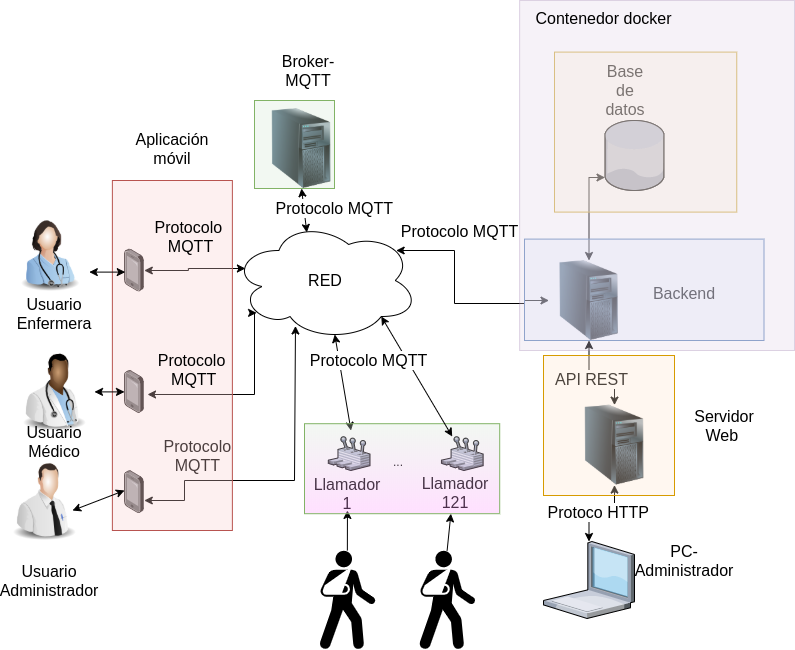
\includegraphics[scale=.45]{./Figures/DiagramaSistemaOrganizado.png}
	\caption{División del sistema.}
	\label{fig:División del sistema}
\end{figure}



\pagebreak

\section{Descripción del protocolo MQTT}
\label{sec:Descripción del protocolo MQTT}

MQTT fue introducido en 1999 por IBM y Eurotech. Es un protocolo de mensajería por suscripción/publicación especialmente diseñado para la comunicación M2M(\textit{Machine to Machine}, Máquina a Máquina) en dispositivos con bajos recursos \citep{WEBSITE:5} .

Para poder explicar el funcionamiento del protocolo es necesario incorporar conceptos definidos en la especificación \citep{WEBSITE:5}:

\begin{itemize}
\item Mensaje: datos transmitidos mediante el protocolo MQTT  a través de la red por la aplicación. Cuando un mensaje es transmitido, el mismo contiene datos útiles(\textit{"payload"}), un campo que identifica la Calidad de Servicio (\textit{Quality of Service}, QoS), ciertas propiedades y un nombre de tópico.
\item Cliente: programa o dispositivo que utiliza MQTT.
\item Servidor o Broker: programa o dispositivo que actúa como intermediario entre clientes que publican mensajes y clientes que han realizado suscripciones.
\item Sesión: una interacción entre cliente y servidor con estados bien definidos.
\item suscripción: una  suscripción implica un filtrado de tópicos y una máxima calidad de servicio. Una suscripción está asociada a una sola sesión y una sesión puede poseer varias suscripciones.
\item Nombre de tópico: etiqueta que se adjunta a un mensaje la cual es comparada con las suscripciones conocidas en el servidor.
\item Filtro de tópico: es una expresión contenida dentro de la suscripción para indicar interés, por parte del cliente, en uno o más tópicos.
\item Suscripción con comodín o \textit{Wildcard} : es una expresión contenida dentro de la suscripción que contiene un carácter especial o comodín, como ser '+' o '\# ', que representan un nivel único y nivel múltiple respectivamente.

\end{itemize}

En este protocolo, el funcionamiento es el siguiente: 

Al iniciar la conexión, el cliente envía un mensaje CONNECT al broker y este contesta con un CONNECTACK y un código de estado. El broker mantiene abierta la conexión hasta que el cliente envía un comando de desconexión o la conexión se pierde por algún motivo. Los puertos estándar son 1883 para comunicación no encriptada y 8883 para comunicación encriptada utilizando TLS/SSL \citep{ARTICLE:4}.

Luego el cliente MQTT publica mensajes en un broker MQTT, los cuales son recibidos por los clientes suscriptos o bien retenidos para una futura suscripción \citep{WEBSITE:5}. En la figura \ref{fig:Sistema MQTT} se presentan todos los componentes de una red MQTT:  

\begin{figure}[ht]
	\centering
	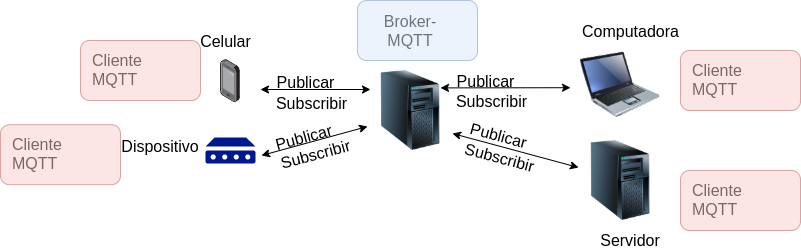
\includegraphics[scale=.45]{./Figures/MQTT-minimal.png}
	\caption{Esquema de un sistema MQTT.}
	\label{fig:Sistema MQTT}
\end{figure}

La conexión MQTT siempre es entre cliente y broker, nunca entre clientes directamente.


Cada mensaje es publicado en una dirección conocida como "tópico". Los clientes pueden subscribirse a múltiples tópicos y recibir todos los mensajes publicados en cada tópico. MQTT es un protocolo binario y normalmente requiere un encabezado fijo de dos \textit{bytes} y un dato útil (\textit{"payload"}) de hasta 256 MB \citep{ARTICLE:2} . 

Ejemplos de tópicos:

\begin{itemize}
\item  1: /user/1/question
\item  2: /user/1/\#
\item  3: /user/+/question
%\item Capítulo 2: Introducción específica
%\item Capítulo 3: Diseño e implementación
%\item Capítulo 4: Ensayos y resultados
%\item Capítulo 5: Conclusiones
\end{itemize}

En el ejemplo 1, en caso de suscribirse a ese tópico, el cliente recibirá todos los mensajes publicados en el subtópico "question".
En el ejemplo 2, el cliente recibirá todos los mensajes dirigidos al usuario 1.
En el ejemplo 3, el cliente que se suscriba a ese tópico recibirá los mensajes enviados a "question" independientemente del número de usuario.


Utiliza usualmente TCP/IP como protocolo de transporte y puede implementar TLS/SLL para seguridad. Por lo que el servicio cliente-broker es del tipo orientado a la conexión. También puede utilizar otros protocolos de red con soporte bidireccional y sin pérdidas de datos \citep{ARTICLE:4} \citep{WEBSITE:5} .


Por otro lado, el protocolo posee tres niveles de calidad de servicio ("QoS", del ingles \textit{Quality of Service}) que permite seleccionar la fiabilidad de la entrega de los mensajes \citep{WEBSITE:5}\citep{WEBSITE:28} :

\begin{itemize}
\item Calidad 0: el mensaje se entrega como máximo una vez, sino no se entrega. Es el modo mas rápido de entrega.
\item Calidad 1: el mensaje se entrega como mínimo una vez. El mensaje se almacena localmente en el emisor y el receptor hasta que se procese. Si no se confirma la recepción se envía de nuevo con el distintivo ''DUP'' establecido hasta que se reciba acuse de recibo.
\item Calidad 2: el mensaje se entrega exactamente una sola vez. El mensaje se almacena localmente en el emisor y el receptor hasta que se procese. El emisor recibe un mensaje acuse de recibo. Si el emisor no recibe un acuse de recibo, el mensaje se envía de nuevo con el distintivo DUP establecido hasta que se reciba un acuse de recibo.
En el segundo par de transmisiones, el remitente indica al destinatario que puede completar el proceso del mensaje, ''PUBREL''. Si el remitente no recibe un acuse de recibo del mensaje ''PUBREL'', el ''PUBREL'' se envía de nuevo hasta que se recibe un acuse de recibo. El remitente suprime el mensaje que ha guardado cuando recibe el acuse de recibo al mensaje “PUBREL” .

El receptor puede procesar el mensaje proporcionado en la primera o segunda fase, no tiene que volver a procesarlo. Si el receptor es un intermediario, publica el mensaje a los suscriptores. Si el receptor es un cliente, el mensaje se entrega a la aplicación de suscriptor. El receptor devuelve un mensaje de finalización al emisor para comunicarle que ha terminado de procesar el mensaje.

\end{itemize}


\label{subsec:WebSockets}
\subsection{Uso de WebSockets en MQTT}

Actualmente no es posible utilizar MQTT natural en un \textit{browser} o navegador debido a la imposibilidad de abrir una conexión TCP pura. 

Una solución a este problema puede ser transmitir el mensaje MQTT sobre una conexión WebSocket lo que permite que un \textit{browser} pueda utilizar todas las características del protocolo directamente. Esto es muy útil en el caso de las aplicaciones de telefono móvil \citep{WEBSITE:6}. 


WebSocket es un protocolo de red que provee comunicación bidireccional entre un \textit{browser} y un servidor web. El protocolo fue estandarizado en 2011 y es soportado por todos los navegadores modernos. Como MQTT, el protocolo WebSocket está basado en TCP. En la figura \ref{fig:WebSockets MQTT} se muestra conceptualmente como se encapsula la información del protocolo MQTT dentro de una trama WebSocket:

\begin{figure}[ht]
	\centering
	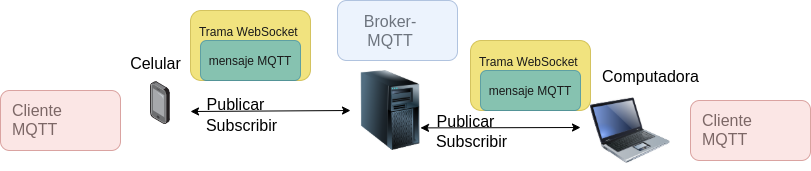
\includegraphics[scale=.45]{./Figures/websocket.png}
	\caption{Uso de WebSockets con MQTT.}
	\label{fig:WebSockets MQTT}
\end{figure}

En MQTT sobre WebSockets, el mensaje MQTT se transfiere a través de la red y es encapsulado por una o más tramas WebSockets. La ventaja de este método de transmisión es que provee una comunicación bi-direcional, ordenada y sin pérdidas \citep{WEBSITE:6} .

Para poder utilizar MQTT sobre WebSockets el Broker debe ser capaz de manejar WebSocket nativos. 

Para mejorar la seguridad, se puede implementar TLS utilizando WebSockets seguros para encriptar toda la conexión.

\label{subsec:Broker Mosquitto}
\subsection{Broker Mosquitto}

Existen muchos brokers MQTT disponibles. Para este trabajo se seleccionó Eclipse Mosquitto como Broker ya que es de código abierto con licencia EPL/EDL que implementa MQTT en sus versiones 5.0, 3.1.1 y 3.1. \citep{WEBSITE:7}.

Otra característica que lo hace muy conveniente es que se encuentra disponible en los repositorios de varias distribuciones de Linux. 




%\label{sec:ejemplo}
%\subsection{Uso de mayúscula inicial para los título de secciones}

%Si en el texto se hace alusión a diferentes partes del trabajo referirse a ellas como capítulo, sección o subsección según corresponda. Por ejemplo: ``En el capítulo \ref{Chapter1} se explica tal cosa'', o ``En la sección \ref{sec:ejemplo} se presenta lo que sea'', o ``En la subsección \ref{subsec:ejemplo} se discute otra cosa''.

%Cuando se quiere poner una lista tabulada, se hace así:

%\begin{itemize}
%	\item Este es el primer elemento de la lista.
%	\item Este es el segundo elemento de la lista.
%\end{itemize}

%Notar el uso de las mayúsculas y el punto al final de cada elemento.

%Si se desea poner una lista numerada el formato es este:

%\begin{enumerate}
%	\item Este es el primer elemento de la lista.
%	\item Este es el segundo elemento de la lista.
%\end{enumerate}

%Notar el uso de las mayúsculas y el punto al final de cada elemento.

%\subsection{Este es el título de una subsección}
%\label{subsec:ejemplo}

%Se recomienda no utilizar \textbf{texto en negritas} en ningún párrafo, %ni tampoco texto \underline{subrayado}. En cambio sí se debe utilizar %\textit{texto en itálicas} para palabras en un idioma extranjero, al menos la primera vez que aparecen en el texto. En el caso de palabras que estamos inventando se deben utilizar ``comillas'', así como también para citas textuales. Por ejemplo, un \textit{digital filter} es una especie de ``selector'' que permite separar ciertos componentes armónicos en particular.

%La escritura debe ser impersonal. Por ejemplo, no utilizar ``el diseño del firmware lo hice de acuerdo con tal principio'', sino ``el firmware fue diseñado utilizando tal principio''. 

%El trabajo es algo que al momento de escribir la memoria se supone que ya está concluido, entonces todo lo que se refiera a hacer el trabajo se narra en tiempo pasado, porque es algo que ya ocurrió. Por ejemplo, "se diseñó el firmware empleando la técnica de test driven development".

%En cambio, la memoria es algo que está vivo cada vez que el lector la lee. Por eso transcurre siempre en tiempo presente, como por ejemplo:

%''En el presente capítulo se da una visión global sobre las distintas pruebas realizadas y los resultados obtenidos. Se explica el modo en que fueron llevados a cabo los test unitarios y las pruebas del sistema''.

%Se recomienda no utilizar una sección de glosario sino colocar la descripción de las abreviaturas como parte del mismo cuerpo del texto. Por ejemplo, RTOS (\textit{Real Time Operating System}, Sistema Operativo de Tiempo Real) o en caso de considerarlo apropiado mediante notas a pie de página.

%Si se desea indicar alguna página web utilizar el siguiente formato de referencias bibliográficas, dónde las referencias se detallan en la sección de bibliografía de la memoria, utilizado el formato establecido por IEEE en \citep{IEEE:citation}. Por ejemplo, ``el presente trabajo se basa en la plataforma EDU-CIAA-NXP \citep{CIAA}, la cual...''.

%\subsection{Figuras} 

%Al insertar figuras en la memoria se deben considerar determinadas pautas. Para empezar, usar siempre tipografía claramente legible. Luego, tener claro que \textbf{es incorrecto} escribir por ejemplo esto: ``El diseño elegido es un cuadrado, como se ve en la siguiente figura:''

%\begin{figure}[h]
%\centering
%
\includegraphics[scale=.45]{./Figures/cuadradoAzul.png}
%\end{figure}

%La forma correcta de utilizar una figura es con referencias cruzadas, por ejemplo: ``Se eligió utilizar un cuadrado azul para el logo, como puede observarse en la figura \ref{fig:cuadradoAzul}''.

%\begin{figure}[ht]
%	\centering
%	
\includegraphics[scale=.45]{./Figures/cuadradoAzul.png}
%	\caption{Ilustración del cuadrado azul que se eligió para el diseño del logo.}
%	\label{fig:cuadradoAzul}
%\end{figure}

%El texto de las figuras debe estar siempre en español, excepto que se decida reproducir una figura original tomada de alguna referencia. En ese caso la referencia de la cual se tomó la figura debe ser indicada en el epígrafe de la figura e incluida como una nota al pie, como se ilustra en la figura \ref{fig:palabraIngles}.

%\begin{figure}[htpb]
%	\centering
%	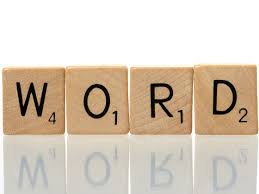
\includegraphics[scale=.3]{./Figures/word.jpeg}
%	\caption{Imagen tomada de la página oficial del procesador\protect\footnotemark.}
%	\label{fig:palabraIngles}
%\end{figure}

%\footnotetext{Imagen tomada de \url{https://goo.gl/images/i7C70w}}

%La figura y el epígrafe deben conformar una unidad cuyo significado principal pueda ser comprendido por el lector sin necesidad de leer el cuerpo central de la memoria. Para eso es necesario que el epígrafe sea todo lo detallado que corresponda y si en la figura se utilizan abreviaturas entonces aclarar su significado en el epígrafe o en la misma figura.



%\begin{figure}[ht]
%	\centering
%	
\includegraphics[scale=.37]{./Figures/questionMark.png}
%	\caption{¿Por qué de pronto aparece esta figura?}
%	\label{fig:questionMark}
%\end{figure}

%Nunca colocar una figura en el documento antes de hacer la primera referencia a ella, como se ilustra con la figura \ref{fig:questionMark}, porque sino el lector no comprenderá por qué de pronto aparece la figura en el documento, lo que distraerá su atención.

%Otra posibilidad es utilizar el entorno \textit{subfigure} para incluir más de una figura, como se puede ver en la figura \ref{fig:three graphs}. Notar que se pueden referenciar también las figuras internas individualmente de esta manera: \ref{fig:1de3}, \ref{fig:2de3} y \ref{fig:3de3}.
 
%\begin{figure}[!htpb]
%     \centering
%     \begin{subfigure}[b]{0.3\textwidth}
%         \centering
%         
\includegraphics[width=.65\textwidth]{./Figures/questionMark}
%         \caption{Un caption.}
%         \label{fig:1de3}
%     \end{subfigure}
%     \hfill
%     \begin{subfigure}[b]{0.3\textwidth}
%         \centering
%         
\includegraphics[width=.65\textwidth]{./Figures/questionMark}
%         \caption{Otro.}
%         \label{fig:2de3}
%     \end{subfigure}
%     \hfill
%     \begin{subfigure}[b]{0.3\textwidth}
%         \centering
%         
\includegraphics[width=.65\textwidth]{./Figures/questionMark}
%         \caption{Y otro más.}
%         \label{fig:3de3}
%     \end{subfigure}
%        \caption{Tres gráficos simples}
%        \label{fig:three graphs}
%\end{figure}

%El código para generar las imágenes se encuentra disponible para su reutilización en el archivo \file{Chapter2.tex}.

%\subsection{Tablas}

%Para las tablas utilizar el mismo formato que para las figuras, sólo que el epígrafe se debe colocar arriba de la tabla, como se ilustra en la tabla \ref{tab:peces}. Observar que sólo algunas filas van con líneas visibles y notar el uso de las negritas para los encabezados.  La referencia se logra utilizando el comando \verb|\ref{<label>}| donde label debe estar definida dentro del entorno de la tabla.

%\begin{verbatim}
%\begin{table}[h]
%	\centering
%	\caption[caption corto]{caption largo más descriptivo}
%	\begin{tabular}{l c c}    
%		\toprule
%		\textbf{Especie}     & \textbf{Tamaño} & \textbf{Valor}\\
%		\midrule
%		Amphiprion Ocellaris & 10 cm           & \$ 6.000 \\		
%		Hepatus Blue Tang    & 15 cm           & \$ 7.000 \\
%		Zebrasoma Xanthurus  & 12 cm           & \$ 6.800 \\
%		\bottomrule
%		\hline
%	\end{tabular}
%	\label{tab:peces}
%\end{table}
%\end{verbatim}


%\begin{table}[h]
%	\centering
%	\caption[caption corto]{caption largo más descriptivo}
%	\begin{tabular}{l c c}    
%		\toprule
%		\textbf{Especie} 	 & \textbf{Tamaño} 		& \textbf{Valor}  \\
%		\midrule
%		Amphiprion Ocellaris & 10 cm 				& \$ 6.000 \\		
%		Hepatus Blue Tang	 & 15 cm				& \$ 7.000 \\
%		Zebrasoma Xanthurus	 & 12 cm				& \$ 6.800 \\
%		\bottomrule
%		\hline
%	\end{tabular}
%	\label{tab:peces}
%\end{table}

%En cada capítulo se debe reiniciar el número de conteo de las figuras y las tablas, por ejemplo, figura 2.1 o tabla 2.1, pero no se debe reiniciar el conteo en cada sección. Por suerte la plantilla se encarga de esto por nosotros.

%\subsection{Ecuaciones}
%\label{sec:Ecuaciones}

%Al insertar ecuaciones en la memoria dentro de un entorno \textit{equation}, éstas se numeran en forma automática  y se pueden referir al igual que como se hace con las figuras y tablas, por ejemplo ver la ecuación \ref{eq:metric}.

%\begin{equation}
%	\label{eq:metric}
%	ds^2 = c^2 dt^2 \left( \frac{d\sigma^2}{1-k\sigma^2} + \sigma^2\left[ d\theta^2 + \sin^2\theta d\phi^2 \right] \right)
%\end{equation}
                                                        
%Es importante tener presente que si bien las ecuaciones pueden ser referidas por su número, también es correcto utilizar los dos puntos, como por ejemplo ``la expresión matemática que describe este comportamiento es la siguiente:''

%\begin{equation}
%	\label{eq:schrodinger}
%	\frac{\hbar^2}{2m}\nabla^2\Psi + V(\mathbf{r})\Psi = -i\hbar %%\frac{\partial\Psi}{\partial t}
%\end{equation}

%Para generar la ecuación \ref{eq:metric} se utilizó el siguiente código:

%\begin{verbatim}
%\begin{equation}
%	\label{eq:metric}
%	ds^2 = c^2 dt^2 \left( \frac{d\sigma^2}{1-k\sigma^2} + 
%	\sigma^2\left[ d\theta^2 + 
%	\sin^2\theta d\phi^2 \right] \right)
%\end{equation}
%\end{verbatim}

%Y para la ecuación \ref{eq:schrodinger}:

%\begin{verbatim}
%\begin{equation}
%	\label{eq:schrodinger}
%	\frac{\hbar^2}{2m}\nabla^2\Psi + V(\mathbf{r})\Psi = 
%	-i\hbar \frac{\partial\Psi}{\partial t}
%\end{equation}

%\end{verbatim}

\section{Descripción del protocolo HTTP}
\label{sec:Descripción del protocolo HTTP}

HTTP es un protocolo que nos permite realizar una petición de datos y recursos como ser documentos HTML que pueden mostrarse en navegadores. Es la base de cualquier intercambio en la red \citep{WEBSITE:19}. En la figura \ref{fig:Protocolo HTTP } se observa donde se ubica el protocolo dentro del modelo de comunicación TCP/IP :


\begin{figure}[ht]
	\centering
	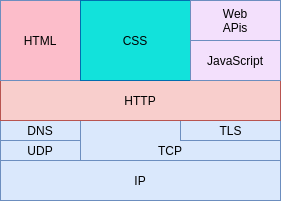
\includegraphics[scale=.5]{./Figures/http.png}
	\caption{Pila de comunicaciones en un navegador.}
	\label{fig:Protocolo HTTP }
\end{figure}

HTTP se basa en el modelo cliente-servidor: las peticiones son enviadas por una entidad al servidor, el cual gestiona y responde.

Entre las características principales figuran \citep{WEBSITE:19}:
\begin{itemize}
\item Es sencillo.
\item Puede expandirse.
\item Es un protocolo de sesiones pero no de estados: no guarda ningún dato entre dos peticiones en la misma sesión.
\item Las conexiones se realizan en la capa de transporte por lo que quedan fuera del protocolo HTTP.
\end{itemize}

La secuencia de la comunicación entre el cliente y el servidor es la siguiente \citep{WEBSITE:19}:
\begin{enumerate}
\item Se abre conexión TCP: la conexión TCP se utiliza para hacer una petición, o varias, y recibir la respuesta. El cliente puede abrir una conexión nueva, reusar la existente o abrir varias a la vez hacia el servidor.
\item Hacer una peticion HTTP: los mensajes HTTP son legibles en texto plano.
\item Se lee la respuesta enviada por el servidor.
\item Se cierra o reusa la conexión.
\end{enumerate}

En el encabezado del mensaje HTTP se puede introducir información de la sesión. Lo cual resulta muy importante en referencia a la seguridad. 


\section{Sistemas de contenedores Docker}
\label{sec:Docker}

Desde los origenes de la programación, existió una necesidad de abstraer la aplicación desarrollada de la plataforma en la que se ejecuta. Múltiples avances se fueron dando desde ese entonces: sistemas operativos con interfaces de aplicaciones estandar, librerías portables y lenguajes interpretados en máquinas virtuales son algunos de ellos.

Docker es un proyecto de código abierto que permite automatizar el despliegue de aplicaciones dentro de contenedores de software proporcionando una capa de abstracción y automatización. Fue desarrollado por Docker Inc. y su primera versión fue liberada en 2013. Está escrito en el lenguaje Golang y actualmente es un estandar en la industria del Software \citep{WEBSITE:8}.



\begin{figure}[ht]
	\centering
	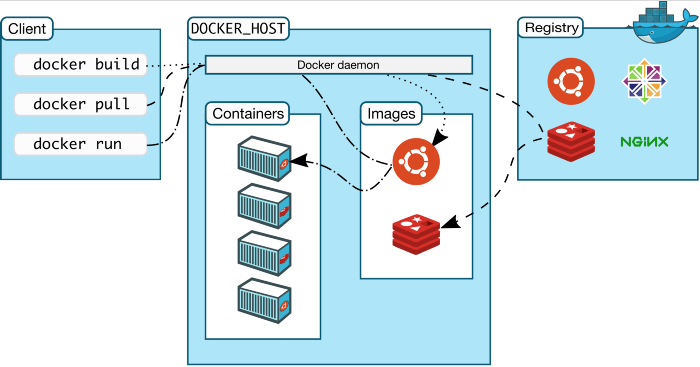
\includegraphics[scale=.5]{./Figures/docker.png}
	\caption{Estructura general de Docker.\protect\footnotemark.}
	\label{fig:Contenedores Docker. }

\end{figure}
\footnotetext{Imagen tomada de \citep{WEBSITE:8}}


Un contenedor de software es un componente aislado que se ejecuta como un proceso mas dentro del sistema operativo del host y posee todas las dependencias y requerimientos que la aplicación necesita para funcionar correctamente. Por cada contenedor en ejecución hay un proceso ejecutandose en el sistema \citep{WEBSITE:8}.

Las partes que componen del ecosistema Docker pueden resumirse de la siguiente manera \citep{WEBSITE:8}\citep{WEBSITE:9}:

\begin{itemize}
\item \textit{Images}: son plantillas que describen el contenedor. Se componen de una base y sobre estas se modifica según necesidad.
\item \textit{Containers}: son instancias de ejecución de una imagen. Se pueden iniciar, detener, mover o eliminar mediante comandos. Se puede conectar un contenedor a una o mas redes.
\item \textit{Networks}: Docker utiliza una interfaz virtual para comunicarse con la red del equipo host.
\item \textit{Volumes}: permiten generar espacios de almacenamiento dentro de cada contenedor, el funcionamiento es similar a las carpetas compartidas en las máquinas virtuales.
\item \textit{Registry}: un registro almacena imágenes de docker. Dockerhub es un registro público que cualquiera puede utilizar.
\end{itemize}

Para poder correr un contenedor docker es necesario ejecutar el comando:
\begin{lstlisting}[label=docker:vControl,caption=Ejecución de contenedor.]  
>docker-run --[parametro1] --[parametro2] ...
nombre_contendor:version
\end{lstlisting}


\subsection{Uso de Docker-compose}
\label{subsec:Docker-compose}

Docker Compose es una herramienta del ecosistema Docker que sirve para definir aplicaciones multicontenedor en un archivo de texto llamado "docker-compose.yml". 
Con esta herramienta se facilita el paso de parámetros al contenedor y posibilita generar imágenes complejas utilizando e interconectando distintos contenedores.

 

\section{Introducción a las bases de datos}
\label{sec: Introducción a las bases de datos}

Se define un dato como un elemento o característica que permite hacer la descripción de un objeto \citep{WEBSITE:12}. En el contexto de los sistemas de Internet de las Cosas, es la mínima expresión de información que se puede gestionar.

Una base de datos es una colección de datos (o información) organizados, estructurados y almacenados electrónicamente en un sistema de computadoras. En su mayoría son controladas por un DBMS (\textit{database management system}, sistema gestor de bases de datos). Los datos, el DBMS y la aplicación que está asociada a ellos, conforman el llamado sistema de base de datos, o base de datos en forma abreviada \citep{WEBSITE:11}.

Durante los años 80 se popularizó el tipo de base de dato relacional, cuya información se organizaba como un conjunto de tablas con columnas y filas. Este tipo de base de datos provee la forma más eficiente y flexible de acceder a información estructurada.

En 1970, IBM junto a Oracle desarrollaron un lenguaje de programación llamado SQL (\textit{Structured Query Language}, Lenguaje de Colas Estructurado). Su principal objetivo era manipular, encolar, definir datos y proveer control de acceso en las bases de datos relacionales. Este lenguaje es apliamente utilizado hoy en día, aún cuando surgen nuevos.

Se podría empezar a clasificar las bases de datos en relacionales y no relacionales. Las primeras utilizan SQL como su lenguaje de programación y entre ellas podemos encontrar: PostgreSQL, MySQL y SQL Server. Las segundas no utilizan un lenguaje SQL, ya que no trabajan en base a estructuras definidas, poseen una gran escalabilidad y estan diseñadas para manejar grandes volumentes de datos \citep{WEBSITE:12}.


\subsection{Descripción de MySQL}
\label{subsec: Bases de datos relacionales}

En este trabajo se seleccionó el DBMS MySQL. Es un sistema de gestión de bases de datos con mas de 10 millones de instalaciones. Fue desarrollado a mediados de la década de los 90, y es de uso libre. Es potente, rápido y altamente escalable \citep{BOOK:2}.

Existen tres formas de interactuar con una base de datos MySQL: utilizando la consola, a través de una interfaz web como phpMyAdmin y mediante un lenguaje de programación.

En la figura \ref{fig:Página phpMyAdmin} se puede observar la interfaz:

 
\begin{figure}[ht]
	\centering
	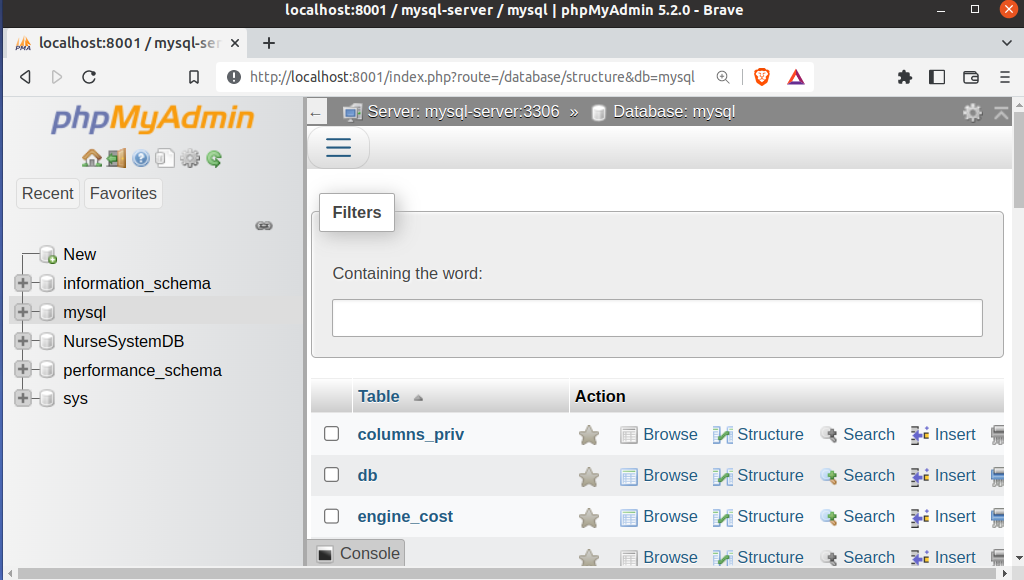
\includegraphics[scale=.35]{./Figures/phpMyAdmin.png}
	\caption{Página de gestión phpMyAdmin.}
	\label{fig:Página phpMyAdmin}
\end{figure}

Los comandos más utilizados en SQL se observan en la tabla \ref{tab:Funciones SQL} \citep{BOOK:2}:

%\begin{verbatim}
\begin{table}[h]
	\centering
	\caption[Comandos SQL]{Comandos básicos SQL.}
	\begin{tabular}{l c }    
		\toprule
		\textbf{Comando}     & \textbf{Función} \\
		\midrule
		ALTER & Modificar una base de datos o una tabla    \\		
		BACKUP    & Copia de seguridad de una tabla      \\
		$\backslash$c  & Cancelar la entrada\\
		CREATE  & Crear la base de datos\\
		DELETE  & Borrar una fila de una tabla\\
		DESCRIBE  & Describir columnas de una tabla\\
		DROP  & Eliminar una base de datos o una tabla\\
		EXIT & Salir.\\
		GRANT & Cambiar permisos de un usuario\\
		INSERT INTO..VALUES & Insertar datos\\
		RENAME & Cambiar nombre de una tabla\\
		USE & Usar una base de datos\\
		UPDATE & Actualizar un registro existente\\
		SELECT  & Consultar una fila\\
		JOIN... ON & Consultar múltiples tablas\\
		\bottomrule
		\hline
	\end{tabular}
	\label{tab:Funciones SQL}
\end{table}
\pagebreak
Ejemplo de uso, suponiendo 2 tablas:

\begin{table}[h]
	\centering
	\caption[Tabla 1 Ejemplo SQL]{TABLA1 para el ejemplo 1.}
	\begin{tabular}{l c c}    
		\toprule
		\textbf{PacienteId}     & \textbf{Nombre} \\
		\midrule
		 1& Pedro    \\		
 		 2& Juan    \\				
		\bottomrule
		\hline
	\end{tabular}
	\label{tab:Ejemplo 1}
\end{table}

\begin{table}[h]
	\centering
	\caption[Tabla 2 Ejemplo SQL]{TABLA2 para el ejemplo 1.}
	\begin{tabular}{l c c}    
		\toprule
		\textbf{PacienteId}     & \textbf{Apellido} \\
		\midrule
		 1& Perez    \\		
 		 2& Salvador    \\	
		\bottomrule
		\hline
	\end{tabular}
	\label{tab:Ejemplo 2}
\end{table}

Si se quiere obtener el nombre y apellido del paciente con pacienteId igual a 1, una forma de obternerlo es ejecutando el código:

\begin{lstlisting}[label=código:SQL:vControl,caption=Ejecución de comando sql]  
>SELECT Nombre,Apellido FROM TABLA1 as TB1 \
JOIN TABLA2 as TB2 ON TB1.pacienteId=TB2.pacienteId \
WHERE TB1.pacienteId=1;
>Pedro Perez
\end{lstlisting}

Una de las múltiples ventajas que poseen los motores de bases de datos relacionales es la posibilidad de realizar transacciones. Las mismas consisten en secuencias de operaciones que se ejecutan en orden y se completan con éxito.

\begin{lstlisting}[label=código:SQL2:vControl,caption=Secuencia de transacción SQL.]  
>BEGIN;
>SELECT Nombre FROM  TABLA1;
>SELECT Apellido FROM  TABLA2;
>COMMIT;
>Pedro 
>Juan
>Perez
>Salvador
\end{lstlisting}


\section{Frameworks/librerías para desarrollo web/móvil}

En esta sección se presentan las librerías y frameworks que se utilizaron para el desarrollo.

\subsection{Librerías Node.js, Express y JWT}
\label{subsec: Node}
El trabajo realizado utiliza como lenguaje de programación  Javascript para las tareas del backend. Para generar el servidor se utiliza Node.js \citep{WEBSITE:20}, que es un \textit{runtime environment}(entorno de ejecución) de Javascript. Node.js se encuentra orientado a eventos asíncronos y está diseñado para crear aplicaciones de red escalables.

Ademas de la alta velocidad de ejecución, Node.js posee un bucle de eventos (\textit{Event loop}), que permite gestionar múltiples clientes de forma asíncrona. La principal ventaja que posee el método de bucle de eventos de Node.js con respecto al método tradicional (que se valían de programación basada en hilos) es que no escala la cantidad de memoria a utilizar a medida de que se aumentan las conexiones.

Por ultimo, es importante mecionar que Node.js posee un gestor de paquetes/librerías llamado NPM, que permite fácilmente incorporar piezas de software probadas a los proyectos.


Para el ruteo de los endpoints con los que se comunica la página web se utiliza Express.js \citep{WEBSITE:21} que es una infraestructura web rápida, minimalista y flexible para Node.js. 

Express.js facilita la creación de la API(\textit{Application Program Interface}, Interfaz de Programación de Aplicaciones), asi como la incorporación de software \textit{Middleware}. 

Con respecto a la seguridad para el acceso de la página web, existen dos métodos: por medio de \textit{cookies} o por medio de web \textit{tokens}. Se seleccionó utilizar el segundo y para ello se utiliza JWT \citep{WEBSITE:22} que implementa el estandar RFC 7519. 



\subsection{Framework Ionic/Angular, Capacitor y Android Studio}
\label{subsec: Ionic}

Drifty.co introdujo Ionic en el año 2013 \citep{WEBSITE:24}. Nació originalmente para desarrollar aplicaciones móviles con Angular 1 pero hoy en día permite desarrollar para dispositivos celulares, páginas web progresivas y aplicaciones de escritorio junto con Electron \citep{WEBSITE:25}. Ionic permite trabajar con Vue, React y Angular en su última versión.

Este framework posee muchos \textit{plugins}(o software de ayuda) que permiten acceder a los recursos de los dispositivos móviles como ser su micrófono, la cámara, la información de posicionamiento, entre otros. Junto con Ionic se utiliza Capacitor \citep{WEBSITE:26}, que es un runtime nativo para iOS, Android y aplicaciones web progresivas.

El código que genera Ionic debe compilarse para generar el archivo ejecutable(ya sea .ipa para iOS o .apk para Android). Para ello, se utilizan los entornos de desarrollo Xcode para iOS, y Android Studio para Android.

Por ejemplo, el método de desarrollo para una aplicación que se ejecutará en un dispositivo Android es el siguiente:

\begin{enumerate}
\item Desarrollo: se genera el código fuente en una pc.
\item Prueba virtual en el navegador:  se realiza debug localmente, utilizando los comandos ionic serve o ionic-lab
\item Prueba en el disposito: se genera un \textit{build}(construcción de software) y se carga Android Studio. Luego se descarga en el dispositivo.
\end{enumerate}
 
%	\chapter{Diseño e implementación} % Main chapter title
\label{Chapter3} 

En este capítulo se explica como se utilizaron las herramientas mencionadas en el capítulo 2 para resolver los objetivos del trabajo presentados en el capítulo 1.

% Change X to a consecutive number; for referencing this chapter elsewhere, use \ref{ChapterX}

\definecolor{mygreen}{rgb}{0,0.6,0}
\definecolor{mygray}{rgb}{0.5,0.5,0.5}
\definecolor{mymauve}{rgb}{0.58,0,0.82}

%%%%%%%%%%%%%%%%%%%%%%%%%%%%%%%%%%%%%%%%%%%%%%%%%%%%%%%%%%%%%%%%%%%%%%%%%%%%%
% parámetros para configurar el formato del código en los entornos lstlisting
%%%%%%%%%%%%%%%%%%%%%%%%%%%%%%%%%%%%%%%%%%%%%%%%%%%%%%%%%%%%%%%%%%%%%%%%%%%%%
\lstset{ %
  backgroundcolor=\color{white},   % choose the background color; you must add \usepackage{color} or \usepackage{xcolor}
  basicstyle=\footnotesize,        % the size of the fonts that are used for the code
  breakatwhitespace=false,         % sets if automatic breaks should only happen at whitespace
  breaklines=true,                 % sets automatic line breaking
  captionpos=b,                    % sets the caption-position to bottom
  commentstyle=\color{mygreen},    % comment style
  deletekeywords={...},            % if you want to delete keywords from the given language
  %escapeinside={\%*}{*)},          % if you want to add LaTeX within your code
  %extendedchars=true,              % lets you use non-ASCII characters; for 8-bits encodings only, does not work with UTF-8
  %frame=single,	                % adds a frame around the code
  keepspaces=true,                 % keeps spaces in text, useful for keeping indentation of code (possibly needs columns=flexible)
  keywordstyle=\color{blue},       % keyword style
  language=[ANSI]C,                % the language of the code
  %otherkeywords={*,...},           % if you want to add more keywords to the set
  numbers=left,                    % where to put the line-numbers; possible values are (none, left, right)
  numbersep=5pt,                   % how far the line-numbers are from the code
  numberstyle=\tiny\color{mygray}, % the style that is used for the line-numbers
  rulecolor=\color{black},         % if not set, the frame-color may be changed on line-breaks within not-black text (e.g. comments (green here))
  showspaces=false,                % show spaces everywhere adding particular underscores; it overrides 'showstringspaces'
  showstringspaces=false,          % underline spaces within strings only
  showtabs=false,                  % show tabs within strings adding particular underscores
  stepnumber=1,                    % the step between two line-numbers. If it's 1, each line will be numbered
  stringstyle=\color{mymauve},     % string literal style
  tabsize=2,	                   % sets default tabsize to 2 spaces
  title=\lstname,                  % show the filename of files included with \lstinputlisting; also try caption instead of title
  morecomment=[s]{/*}{*/}
}


%----------------------------------------------------------------------------------------
%	SECTION 1
%----------------------------------------------------------------------------------------
\section{Generación del entorno base para el desarrollo del sistema de backend}
\label{Generación del entorno base para el desarrollo del sistema de backend}
 En esta sección se presentan las distintas partes que componen el sistema.
La solución fue concebida como un sistema distribuido, por lo que la página web de configuración, el backend, el \textit{broker} y las aplicaciones móviles pueden estar en distintos dispositivos físicamente. La única condicion necesaria es que se encuentren en una red que permite la conexión entre ellos. La red puede ser una red local (implementada con router ) o bien internet.
La aplicación web utiliza HTTP para interactuar con el backend y las aplicaciones móviles utilizan MQTT.
%La idea de esta sección es resaltar los problemas encontrados, los criterios utilizados y la justificación de las decisiones que se hayan tomado.

%Se puede agregar código o pseudocódigo dentro de un entorno lstlisting con el siguiente código:

%\begin{verbatim}
%\begin{lstlisting}[caption= "un epígrafe descriptivo"]
%	las líneas de código irían aquí...
%\end{lstlisting}
%\end{verbatim}

%A modo de ejemplo:

%\begin{lstlisting}[label=cod:vControl,caption=Pseudocódigo del lazo principal de control.]  % Start your code-block

%#define MAX_SENSOR_NUMBER 3
%#define MAX_ALARM_NUMBER  6
%#define MAX_ACTUATOR_NUMBER 6

%uint32_t sensorValue[MAX_SENSOR_NUMBER];		
%FunctionalState alarmControl[MAX_ALARM_NUMBER];	//ENABLE or DISABLE
%state_t alarmState[MAX_ALARM_NUMBER];						//ON or OFF
%state_t actuatorState[MAX_ACTUATOR_NUMBER];			//ON or OFF

%void vControl() {

%	initGlobalVariables();
	
%	period = 500 ms;
		
%	while(1) {

%		ticks = xTaskGetTickCount();
		
%		updateSensors();
		
%		updateAlarms();
		
%		controlActuators();
		
%		vTaskDelayUntil(&ticks, period);
%	}
%}
%\end{lstlisting}


\section{Broker Mosquitto}
\label{Broker Mosquitto}

El broker Mosquitto es una parte central del sistema ya que se encarga de distribuir los mensajes entre los distintos elementos. El único requisito es que se encuentre instalado en la misma red que los clientes (en un dispositivo que no requiere de muchos recursos). Su instalación, en un entorno operativo Ubuntu se realiza con los siguientes comandos:


\begin{lstlisting}[caption=  Instalación/lanzamiento del broker Mosquitto]
		sudo apt-get install mosquitto mosquitto-clients
		sudo systemctl enable mosquitto.service
\end{lstlisting}

Para configurarlo se debe editar el archivo : "/etc/mosquitto/mosquitto.conf", donde se especifica el puerto que se utiliza, en este caso, el puerto 9001 con el protocolo Websockets. Se permite la interconexión de cualquier cliente y el archivo donde se guarda el log de todos los eventos se encuentra en la ubicación "/var/log/mosquitto/mosquitto.log".

\begin{lstlisting}[label=cod:mosquitto.conf,caption=  Contenido archivo mosquitto.conf.]
log_dest file /var/log/mosquitto/mosquitto.log

include_dir /etc/mosquitto/conf.d
listener 9001
protocol websockets
allow_anonymous true

\end{lstlisting}



\pagebreak
\section{Sistema Docker}

Para iniciar el contenedor \textit{Docker} se ejecuta el comando : ''\textit{Docker-compose up}''.  Este comando busca en el archivo docker-compose.yml la información de los distintos servicios que debe inicializar y su configuración.

Los siguientes servicios son instalados:

\begin{itemize}
\item servidor mysql: se utiliza la imagen: 5.7. Utiliza el puerto 3036 para las comunicaciones. 
\item servidor mysql-admin: se utiliza la imagen: phpmyadmin/phpmyadmin. Se configura el puerto 8001:80 para servir la aplicación.
\item backend node: se utiliza la imagen abassi/nodejs-server:10.0-dev.
\end{itemize}

Por otra parte, se configura una red interna NurseSystem-net que hace de \textit{bridge} (puente) con la red del sistema host.



\section{Base de datos del sistema}
En esta sección se describen las distintas tablas que se almacenan en la base de datos y son útiles para el sistema.  

\begin{enumerate}

\item Tabla usuarios (\textit{User}): tabla que contiene la información de los usuarios del sistema. El campo id se incrementa automáticamente, es decir, al incorporar un nuevo usuario al sistema la base de datos asigna el id (se utiliza este campo como llave primaria). En el campo contraseña se almacena el hash de la misma (generado con Bcrypt \citep{WEBSITE:31}). El campo ocupación representa la actividad a la que se dedica el usuario en el establecimiento y puede tomar uno de los siguientes valores: ''Enfermero'',''Médico'' o ''Administrador''. El campo estado (\textit{State}) se utiliza en versiones posteriores del sistema. La estructura de la tabla se presenta en la figura \ref{fig:Tabla Usuarios (base de datos)}.

\begin{figure}[ht]
	\centering
	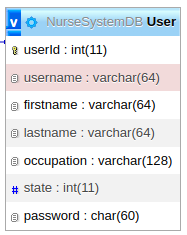
\includegraphics[scale=.70]{./Figures/dB(user).png}
	\caption{Tabla Usuarios.}
	\label{fig:Tabla Usuarios (base de datos)}
\end{figure}

\item Tabla Camas (\textit{Bed}): tabla que contiene la siguiente información de las camas: su identificación (como en el item anterior se incrementa automáticamente y es clave primaria), ubicación (piso y cuarto) y el número de dispositivo llamador. La estructura de la tabla se presenta en la figura \ref{fig:Tabla Camas (base de datos)}.

\begin{figure}[ht]
	\centering
	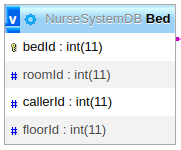
\includegraphics[scale=.70]{./Figures/dB(bed).png}
	\caption{Tabla Camas.}
	\label{fig:Tabla Camas (base de datos)}
\end{figure}
\pagebreak
\item Tabla Paciente (\textit{Patient}): tabla que contiene la información de los pacientes. En esta tabla el id no se incrementa automáticamente (ya que es asignado manualmente por el administrador). Ademas, los campos \textit{bedId}, \textit{notesTableId} y \textit{userTableId} contienen claves foraneas que identifican un elemento de la tabla
\textit{Bed} (cama), \textit{notesTable} (tablas de notas) y \textit{userTable} (tablas de médicos relacionados al paciente). La estructura de la tabla se presenta en la figura \ref{fig:Tabla pacientes (base de datos)}.


\begin{figure}[ht]
	\centering
	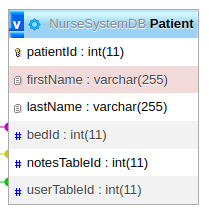
\includegraphics[scale=.70]{./Figures/dB(patient).png}
	\caption{Tabla pacientes.}
	\label{fig:Tabla pacientes (base de datos)}
\end{figure}


\item Relación médicos-pacientes : para generar la relación se utilizan un par de tablas intermedias que permiten que un mismo paciente posea varios médicos asignados. Además, un paciente puede utilizar a los mísmos médicos de otro paciente. Se presenta la relación en la figura \ref{fig:Relación médicos-pacientes}.
\begin{figure}[ht]
	\centering
	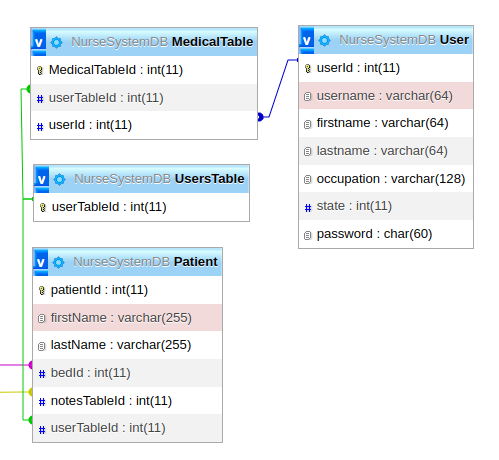
\includegraphics[scale=.65]{./Figures/tabla-medicos-pacientes.png}
	\caption{Relación médicos-pacientes.}
	\label{fig:Relación médicos-pacientes}
\end{figure}
\item Relación tabla de notas-pacientes: como en el caso anterior, se utiliza una tabla de notas generales con una tabla intermedia que los indexa. En este caso, y como es particular de cada paciente, no se puede repetir.  Se presenta la relación en la figura \ref{fig:Relación notas-pacientes (base de datos)}.
\begin{figure}[ht]
	\centering
	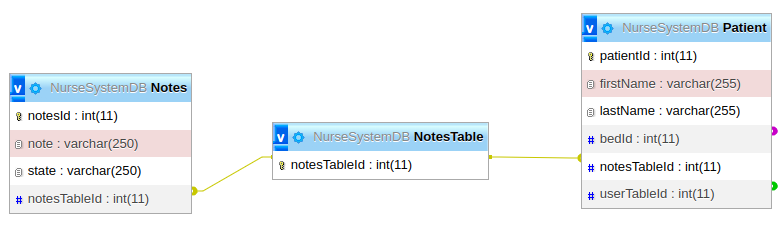
\includegraphics[scale=.65]{./Figures/patient-notes.png}
	\caption{Relación notas-pacientes.}
	\label{fig:Relación notas-pacientes (base de datos)}
\end{figure}


\pagebreak




\item Tabla de eventos programados: En esta tabla se cargan las tareas programadas para un paciente. Se representa en la figura \ref{fig:Tabla de eventos programados (base de datos)} y sus campos son los siguientes:
\begin{itemize}
\item eventId: identificador de evento, se auto incrementa.
\item patientId: número de paciente, es asignado por el cliente y hace referencia a la identificación del paciente
\item type: tipo de evento, puede ser \textit{diario}, \textit{mensual} o \textit{anual} 
\item Datetime: momento que se requiere que se realice la acción.
\item Nota: es donde se coloca la tarea a realizar (Por ejemplo, suministrar X gramos de medicamento Y).
\end{itemize}


\begin{figure}[ht]
	\centering
	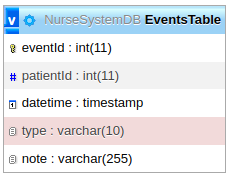
\includegraphics[scale=.70]{./Figures/Events.png}
	\caption{Tabla de eventos programados.}
	\label{fig:Tabla de eventos programados (base de datos)}
\end{figure}

\item Tabla de log eventos: En esta tabla se guardan los eventos relacionados con un paciente. Su estructura se muestra en \ref{fig:Tabla de registro de eventos (base de datos)} y sus componentes son:
\begin{itemize}
\item logEventId: se asigna al guardarse el evento.
\item type: el tipo puede ser \textit{tarea programada} o \textit{llamada paciente}. 
\item pacientId: identificador del paciente. 
\item userId: identificador del usuario que finalizó la tarea. 
\item Nota: en el caso de tarea programada, se guarda la nota de la tarea.
\item Nota2: se cargan por el usuario que finalizó la acción al escribir la memoria de lo realizado.
\end{itemize}



\begin{figure}[ht]
	\centering
	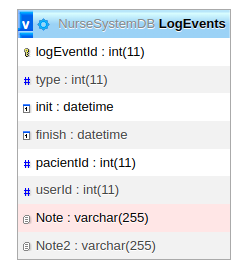
\includegraphics[scale=.70]{./Figures/logEvents.png}
	\caption{Tabla de registro de eventos.}
	\label{fig:Tabla de registro de eventos (base de datos)}
\end{figure}

\item Tabla de especialidades (\textit{SpecTable}): En esta tabla se presentan las distintas especialidades que poseen los enfermeros. Cada especialidad es un tratamiento que puede ser asignado a un paciente.

\item Tabla de especialidades de enfermeros (\textit{NurseSpecTable}): En esta tabla se relacionan a los enfermeros con su Id y las distintas especialidades que pueden realizar. Un enfermero puede poseer más de una especialidad.

\item Tabla de tratamientos de pacientes (\textit{PatientSpecTable}): En esta tabla se relacionan a los pacientes con su Id y un tratamiento (se obtiene de la SpecTable). 

\item Tabla de códigos QR (\textit{QRbed}): En esta tabla se almacenan, en formato texto, los códigos QR correspondientes a las camas para su reconocimiento.

\item Tabla de prioridades (\textit{PriorityTable}): En esta tabla el administrador puede asignar prioridades a las distintas camas del sistema.  Las prioridades son de 5 niveles, siendo 5 la más alta prioridad.



\end{enumerate}



\section{Sistema de gestión}

El backend se diseñó fragmentándolo en tres partes:

\begin{itemize}
\item Módulo de monitoreo: clases que ayudan a publicar a todos los clientes MQTT los estados del sistema (usuario logeados y estados de habitaciones/pacientes). 
\item Módulo de respuestas al cliente página web: expone una API para que los administradores del sistema puedan incorporar usuarios, pacientes, camas, observar estadísticas, etc.
\item Módulo de respuestas al cliente MQTT: se subscribe a los tópicos correspondientes para responder consultas.
\end{itemize}

En la figura \ref{fig:Estructura de carpetas (backend)} se presenta la estructura de directorios del backend.

\begin{figure}[ht]
	\centering
	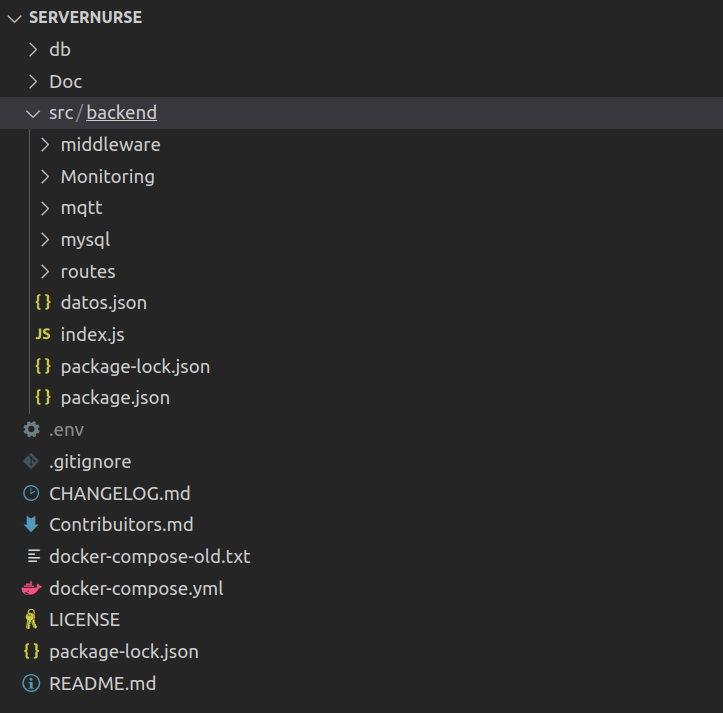
\includegraphics[scale=.45]{./Figures/projectStructure.png}
	\caption{Estructura de carpetas (backend).}
	\label{fig:Estructura de carpetas (backend)}
\end{figure}

La descripción de los contenidos de cada carpeta es:
\begin{itemize}
\item middleware: contiene el programa que filtra el acceso a la API desde  la página web.
\item Monitoring: contiene clases con información del estado del sistema que se actualiza cada cierto tiempo. Cada una de estas clases contiene una lista de todos los elementos y se presenta a los tópicos correspondientes.
\item mqtt: contiene clases que se encargan de procesar y responder los mensajes que se reciben por medio del protocolo MQTT.
\item mysql: contiene la clase con el \textit{pool} (''grupo'') de conexiones a la base de datos. El objetivo es poder reutilizar conexiones por distintos usuarios.
\item routes: contiene las rutas de express para acceder a la base de datos desde las peticiones por HTTP.
\end{itemize}

\pagebreak
\subsection{Descripción de las clases para monitoreo del sistema}

Las siguientes son las clases que se utilizan para reportar mediante MQTT los estados del sistema. Para resumir se presentan los elementos principales, pero no las funciones que las componen.

\begin{itemize}

\item \textit{ Monitoreo de camas} (código \ref{cod:bedlist}):\\
La clase \textit{Bedslist} contiente una lista de elementos JSON con información de cada cama (se instancia al iniciar el backend).

\begin{lstlisting}[label=cod:bedlist,caption=  Clase Bedlist.]
class  BedsList  {    
    constructor() {
         this.bedlist=[{id:0,st:0,spec:0}];                        
    }
...}
\end{lstlisting}

Los componentes de cada elemento son 
\begin{enumerate}
\item id: identificador de cama.
\item st: estado de la cama. Los valores que puede poseer este campo son: 
\begin{itemize}
\item 0: no ocupada.
\item 1: ocupada.
\item 2: llamando paciente.
\item 3: llamada aceptada por enfermero.
\item 4: enfermero atendiendo.
\item 5: tarea programada.
\item 6: enfermero solicitando ayuda.
\end{itemize}
\item spec: número de tratamiento del paciente en la cama (es utilizado por los clientes enfermeros para filtrar si pueden o no atenderlo).
\end{enumerate}


\item \textit{ Monitoreo de usuarios} (código \ref{cod:Userlist}):\\
La clase\textit{UserList} contiente una lista de elementos JSON con información de cada usuario (se instancia al iniciar el backend):

\begin{lstlisting}[label=cod:Userlist,caption=  Clase Userlist.]
class  UserList  {   
constructor() {
         this.UserList=[{id:0,st:0}];                
        
    }
...}
\end{lstlisting}

Los componentes de cada elemento son 
	\begin{enumerate}
		\item id: identificador de usuario.
		\item st: estado de usuario. Puede poseer los siguientes estados: 
			\begin{itemize}
				\item 0: no logeado.
				\item 1: logeado.
			\end{itemize}
	\end{enumerate}




\item \textit{ Monitoreo de eventos programados} (código \ref{cod:Calendarlist}):\\
La clase se utiliza para presentar a los clientes las notas de las tareas programadas que se lanzan. Es una lista que se vacía cuando la tarea finaliza (sirve para mantener ordenadas las tareas programadas).

\begin{lstlisting}[label=cod:Calendarlist,caption=  Clase CalendarList.]
class  Calendarlist  {   
constructor() {
         this.CalendarList=[{calendarId:0,bedId:0,note:null}];                
        
    }
...}
\end{lstlisting}

Los componentes de cada elemento son 
	\begin{enumerate}
		\item calendarId: identificador de evento.
		\item bedId: número de cama.
		\item note: Nota de la tarea (obtenida de la base de datos).		

	\end{enumerate}



\pagebreak
\item \textit{ Monitoreo de paciente-usuario-tipo de evento} (código \ref{cod:BedUserlist}):\\
La clase BedUserlist se utiliza para saber quien está atendiendo, en todo momento, a un paciente.

\begin{lstlisting}[label=cod:BedUserlist,caption=  Clase BedsUserList.]
class  BedUserlist  { 
 constructor() {
         this.beduserlist=[{bedId:0,userId:0,type:0}];                        
    }
...}
\end{lstlisting}

Los componentes de cada elemento son 
	\begin{enumerate}
		\item bedId: número de cama.
		\item userId: número de usuario.
		\item type: tipo de evento: 
		\begin{itemize}
			\item provocado por un paciente
			\item visita programada		
		\end{itemize}		 	

	\end{enumerate}


\end{itemize}
\subsection{Descripción de API MQTT para la mensajería de la aplicación móvil}

En esta sección se describe los módulos que permiten la interacción del sistema con los clientes utilizando el protocolo MQTT.


El módulo principal es mqtt.js (dentro de la carpeta mqtt) y contiene la inicialización de la conexión inicial al broker, el lanzamiento de las tareas de monitoreo (publicación de las listas antes definidas en los tópicos específicos) y la escucha de los mensajes. Una vez recibido un mensaje, dependiendo del tipo, se deriva a la clase correspondiente que realiza el tratamiento acorde a la petición. En el fragmento de código  \ref{cod:Tareas MQTT} se presentan las tareas de inicialización del módulo.



\begin{lstlisting}[label=cod:Tareas MQTT,caption=  Tareas ejecutadas por mqtt.js.]
var client = mqtt.connect(process.env.MQTT_CONNECTION)
//listening to  messages
client.on('connect', function () {
  client.subscribe('/User/#', function (err) {
    if (err) {
    console.log("error:"+err);
    }
  })

  client.subscribe('/Pacient/#', function (err) {
    if (err) {      
      console.log("error:"+err);
    }
  })
  client.subscribe('/Beds/#', function (err) {
    if (err) {      
      console.log("error:"+err);
    }
  })







  //task that will publish beds state each second
  setInterval(publishBedStates, 10000);
  //task that will publish users state 
  setInterval(publishUserStates, 15000);
})
\end{lstlisting}

El sistema recibe mensajería por medio de tres tópicos principales: \textit{User}, \textit{Pacient} y \textit{Beds}, según se observa en las lineas 4, 10 y 15 de \ref{cod:Tareas MQTT}. Por otra parte, se utilizan variables de entorno como ser \textit{MQTT\textunderscore CONNECTION}, que contiene informacion de la IP del broker y el puerto.

Por último, dentro de esta función se setean dos temporizadores para ejecutar las funciones publishBedStates y publishUserStates que publican los listados de los estados de camas y usuarios cada cierto tiempo.




El contenido útil (\textit{payload}) de los mensajes MQTT tiene la siguiente forma:

\begin{lstlisting}[label=cod:Mensaje MQTT,caption=  Formato mensaje MQTT.]

payload={_username: "xxxx",_content: "xxx", _bedId: xx, _type: x}

\end{lstlisting}

La descripción de los campos es la siguiente:
\begin{itemize}
\item \textunderscore username: nombre del usuario que envió el comando.
\item \textunderscore content: contenido.
\item \textunderscore bedId: número de cama a la que se hace referencia.
\item \textunderscore type: tipo de mensaje.
\end{itemize}

El tipo de mensaje permite al sistema derivar las tareas a realizar a las clases correspondientes. En la tabla \ref{tab:Tipos de Mensajes MQTT} se presentan la asignación numérica de cada tipo de mensaje:

%\begin{verbatim}
\begin{table}[h]
	\centering
	\caption[Tipos de mensajes MQTT]{Tipos de mensajes del sistema.}
	\begin{tabular}{l c c}    
		\toprule
		\textbf{Tipo}     & \textbf{Descripción} \\
		\midrule
		1 & Login.    \\		
		2 & Logout.\\
		3 & Escribir nota a paciente.\\
		4 & Solicitar información de paciente de una cama.\\
		5 & Solicitar notas del paciente. \\
		7 & Mensaje de texto entre usuarios.\\
		8 & Solicitar información de cama (ubicación).\\
		9 & Solicitando información de camas de cada médico.\\
		10 & Solicitar información de un paciente de una cama.\\
		11 & Chequeo de QR.\\
		12 & Aceptación de parte de una enfermera.\\
		13 & Finalización de trabajo.\\
		14 & Solicitar ayuda.\\
		16 & Especialización de enfermera.\\
		17 & Consultar tabla de médicos asignada a paciente.\\
		18 & Eliminar nota de paciente.\\
		19 & Cancelar visita.\\
		20 & Notas de evento calendario.\\
		22 & Mensaje de audio entre usuarios.\\
		\bottomrule
		\hline
	\end{tabular}
	\label{tab:Tipos de Mensajes MQTT}
\end{table}
%\end{verbatim}

Las distintas clases que se utilizan son: 
\begin{enumerate}
\item beds: consulta a la base de datos información relacionada a las camas.
\item patient: consulta a la base de datos información relacionada a los pacientes. 
\item users: consulta a la base de datos información relacionada a los usuarios (funciones de logueo y deslogueo).
\item calendar: consulta a la base de datos información relacionada a los eventos programados.
\item nurse: consulta a la base de datos información sobre las especialidades de los enfermeros.
\end{enumerate}

Todas estas clases responden en un tópico correspondiente a los clientes que consultan.

Las excepciones al formato general de los mensajes vienen dadas por:
\begin{itemize}
\item Mensaje de último testamento: informa que un usuario se desconectó. En su \textit{payload} contiene información del nombre de usuario y se publica en el tópico $"/User/Disconnect"$.
\item Mensaje de llamador: informa que un dispositivo llamador fue accionado por un paciente. En su \textit{payload} contiene información del número de llamador y se publica en el tópico $"/Beds/Caller-events"$.

\end{itemize}


\subsection{Descripción de API Rest para aplicación Web}
\label{Descripción de API Rest para aplicación Web}

La API desarrollada utiliza Express junto con Cookie-parser. 
 
En este trabajo se utiliza un \textit{middleware} (capa de software intermedia entre los recursos y la consulta de los usuarios), el cual consiste en una función que realiza el control de acceso a los endpoints. Para lograr la autenticación el backend utiliza las librería \textit{jsonwebtoken} \citep{WEBSITE:32} y \textit{bcrypt} \citep{WEBSITE:31}. En una primera versión, solo se habilita el uso de la página de administración a usuarios administradores.

Se denomina ruteo a la forma que una aplicación express direcciona a las peticiones del cliente a los respectivos módulos que se encargan de su tratamiento.%un \textit{endpoint} de una aplicación responde a las peticiones de los clientes. 
El objeto express posee métodos que realizan las operaciones sobre la base de datos o el sistema. El fragmento de código con las rutas express se observa en el código \ref{cod:Rutas_Express}:

\begin{lstlisting}[label=cod:Rutas_Express,caption=  Rutas express.]
app.use('/api/patient',auth.isAuthenticated,routerPatient);
app.use('/api/user',auth.isAuthenticated,routerUser);
app.use('/api/messages',auth.isAuthenticated,routerMessages);
app.use('/api/notes',auth.isAuthenticated,routerNotes);
app.use('/api/beds',auth.isAuthenticated,routerBeds);
app.use('/api/usersTable',auth.isAuthenticated,routerUsersTable);
app.use('/api/medicalTable',auth.isAuthenticated,routerMedicalTable);
app.use('/api/QR',auth.isAuthenticated,routerQR);
app.use('/api/events',auth.isAuthenticated,routerEvents);
app.use('/api/logEvents',auth.isAuthenticated,routerLogEvents);
app.use('/api/Statistics',auth.isAuthenticated,routerStatistics);
app.use('/api/authentication',routerAuthenticate);
app.use('/api/specTable',auth.isAuthenticated,routerSpecTable);
app.use('/api/nurseSpecTable',auth.isAuthenticated,  routerNurseSpecTable);
app.use('/api/treatment',auth.isAuthenticated,routerPatientSpecTable);
\end{lstlisting}

Brevemente, a continuación, se presenta la funcionalidad de cada endpoint:
\begin{itemize}
\item /api/patient: endpoint que permite la gestión de pacientes (alta, baja, modificación)
\item /api/user: endpoint que permite la gestión de usuarios (alta, baja, modificación)
\item /api/messages: permite obtener un listado de los mensajes entre usuarios (en esta versión de código y debido las limitaciones de almacenamiento del servidor prototipo, se encuentra comentada toda esta funcionalidad)
\item /api/notes: endpoint que permite la gestión de las notas de los pacientes (alta, baja, modificación). 
\item /api/beds: endpoint que permite la gestión de las camas (alta, baja y modificación). 
\item /api/usersTable: endpoint que permite la gestión de las tablas de usuarios. Son las agrupaciones de los médicos que pueden atender a un paciente. 
\item /api/medicalTable: endpoint que permite la gestión de las tablas de tablas de usuarios.
\item /api/QR: enpoint que permite la gestión de los códigos QR (alta, baja y modificación).
\item /api/events: endpoint que permite ingresar una tarea programada al calendario.
\item /api/logEvents: endpoint que permite obtener el listado de eventos.
\item /api/Statistics: endpoint que permite obtener información estadística de la base de datos. Por ejemplo:
\begin{enumerate}
\item número total de visitas de cada enfermero, en formato JSON.
\item número total de llamados de cada paciente, en formato JSON.
\item número de pacientes con igual tratamiento, en formato JSON.
\item número de enfermeras con una especialización, en formato JSON.
\end{enumerate}

Un ejemplo de uso de esta información puede ser: al observarse un incremento de pacientes con cierto tratamiento se puede solicitar capacitar a nuevas enfermeras en esa especialización. Por el contrario, si disminuye un tratamiento se recapacita al personal o bien se lo reduce.

\item /api/authentication: enpoint que permite logearse al sistema. Se explica con más detalle por su importancia.
\item /api/specTable: endpoint que permite modificar la tabla de especialidades de enfermeros (tratamientos para los pacientes). Se permite agregar o quitar especialidades.
\item /api/nurseSpecTable: endpoint que permite asignarle o quitarle especialidades a una enfermera. Por ejemplo, una enfermera recibió una capacitación y desde ese momento queda habilitada para atender pacientes con una cierta necesidad.
\item /api/treatment : endpoint que permite asignar a  un paciente un tratamiento o bien modificar el tratamiento.

\end{itemize}

La ruta authentication se utiliza para entregar un \textit{token} al cliente. En dicha función se verifica que el usuario sea administrador.

\begin{lstlisting}[label=cod:Logueo Web,caption=  Logueo web.]
routerAuthenticate.post('/', async function(req, res) {
    if (req.body) {
        var user = req.body;
        await pool.query('Select username,password,occupation from User WHERE username=?',[user.username], async function(err, result, fields) {
            if (err) {
                var response = JSON.stringify(response_conform);
                res.status(403).send({
                    errorMessage: 'Auth required!'});
                return;    
            }
            else{
                try{
                testUser.username=result[0].username;
                testUser.password=result[0].password;
                }catch (e){res.status(403).send({
                    errorMessage: 'Auth required!'});
                    return;    
                    }
                    await bcrypt.compare(user.password, result[0].password, (err, resultComp)=> {

                        if ((resultComp==true  ) &&(result[0].occupation=="Administrador") ){
                            var token = jwt.sign(user, process.env.JWT_SECRET,{
                                expiresIn: process.env.JWT_EXP_TIM
                            });
                            res.status(200).send({
                                signed_user: result[0],
                                token: token
                            });
                        } else {res.status(403).send({
                                errorMessage: 'Auth required!'
                            }); }
                        })                    
                }      
            }) 
        } else {
            res.status(403).send({
                errorMessage: 'Please provide username and password'
            });
       }

    })

\end{lstlisting}

En el código \ref{cod:Logueo Web} se presenta la función que se encarga de autenticar al usuario. Al recibir un mensaje de autenticación, el backend genera la siguiente secuencia de comprobación:
\begin{enumerate}
\item Verificación que el usuario existe : linea 4
\item Verificación que el password recibido corresponde con el usuairo : linea 21
\item Verificación que el usuario es administrador : linea 21
\end{enumerate}

Luego de eso genera un token que espira luego de un cierto tiempo dado por una variable de entorno y se responde al frontend.

Una vez logueado, la función \textit{auth.isAuthenticated(request,response,next)}, dentro del archivo \textit{./middleware/authentication} comprueba que el usuario que solicita el recurso posea el token correspondiente.
\begin{lstlisting}[label=cod: Autorización,caption=  Control de token.]
exports.isAuthenticated = async(req, res,next)=> {
    let authHeader = (req.headers.authorization || '');
    if (authHeader.startsWith("Bearer ")) {
        token = authHeader.substring(7, authHeader.length);
    } else {
        return res.send({ message: 'No Auth' });
    }
    if (token) {
        jwt.verify(token, process.env.JWT_SECRET, function(err) {
            if (err) {
                console.log("Alguien cambio el token, no es valido");
                return res.json({ message: 'Invalid Token' });
            } else {
                console.log("Validado el token y todo ok");
                return next();
            }
        });
    } else {
        return res.send({ message: 'No token' });
    }
}
\end{lstlisting}

Cada recurso posee su ruta correspondiente. Esta forma de organizar el código permite que se incorporen funcionalidades al backend de forma sencilla.

\pagebreak

\section{Página Web}

La página web de administración consiste en un \textit{dashboard} (tablero de control) que permite al usuario administrador gestionar el sistema.
Fue implementada utilizando el framework Ionic/Angular, con el lenguaje de programación Typescript y las principales secciones de la visualización se observan en la figura \ref{fig:Página web}.

\begin{figure}[ht]
	\centering
	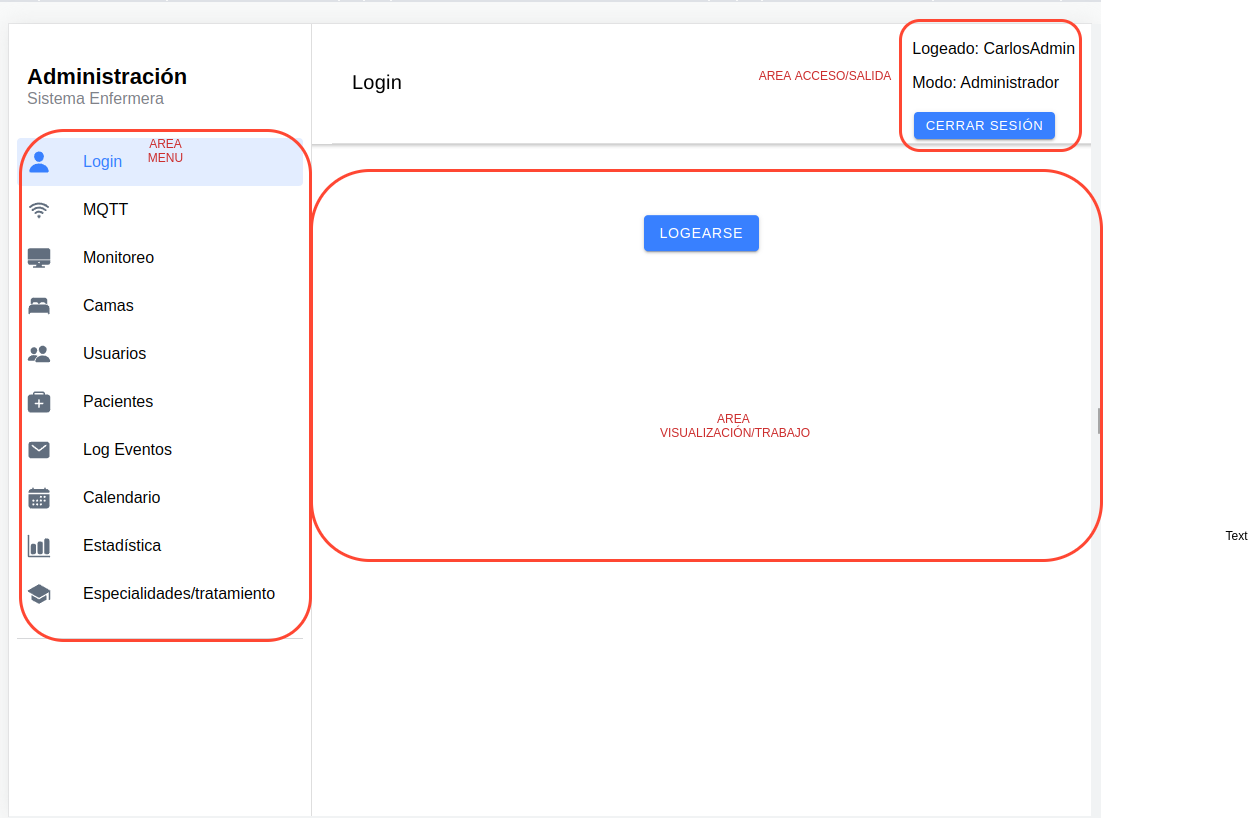
\includegraphics[scale=.40]{./Figures/pagina-web.png}
	\caption{Página web.}
	\label{fig:Página web}
\end{figure}

En el área menú se presentan las distintas utilidades de la página:
\begin{itemize}
\item Login: acceso al sistema. El visitante ingresa su nombre de usuario y contraseña y se le otorga los permisos correspondientes (la conexión recibe el \textit{token} del backend).
\item MQTT: permite editar o probar la conexión al broker MQTT del sistema. Es necesario si se desea monitorear el estado de los usuarios o camas en tiempo real.
\item Monitoreo: se visualiza el estado de las camas o de los usuarios en tiempo real.
\item Camas: permite editar información de las camas como ser código QR, número de llamador, cuarto y piso.
\item Usuarios: permite agregar, editar o dar de baja usuarios.
\item Pacientes: permite agregar, editar o dar de baja pacientes.
\item Log Eventos: permite observar el listado de eventos que se hayan guardado en la base de datos.
\item Calendario: permite observar o agregar tareas rutinarias asignadas a un paciente.
\item Estadísticas: permite observar el número de intervenciones de un enfermero, la distribución de especialidades dentro del grupo de enfermeros y la distribución de tratamientos requeridos por los pacientes. Con esta información el administrador puede notificar sobre necesidades de mayor capacitación en un tema para los enfermeros.
\end{itemize}


\subsection{Estructura y organización del software}

El software web generado contiene dos versiones: una para un entorno de desarrollo y otra para un entorno productivo. En este desarrollo, las características del entorno se encuentran en una carpeta \textit{''/src/environments''}. 

Para ejecutar la aplicación en la máquina local se debe ejecutar el comando:  \textit{'' ionic lab ''}, mientras que para compilar la página productiva se debe ejecutar \textit{'' ionic build prod ''}. El resultado de la construcción se encuentra dentro de la carpeta \textit{''/www''}.

Todo el código de la aplicación se encuentra en la carpeta \textit{''/src/app''} y se presenta una captura en la figura \ref{fig:Carpetas página web.}.


\begin{figure}[ht]
	\centering
	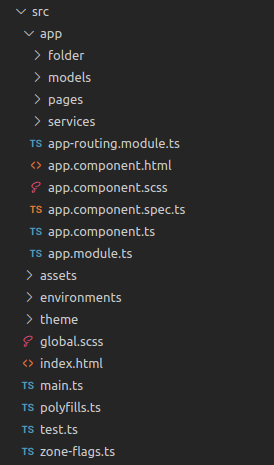
\includegraphics[scale=.60]{./Figures/codigoFront.png}
	\caption{Estructura de carpetas de la aplicación web.}
	\label{fig:Carpetas página web.}
\end{figure}


Dentro de la carpeta \textit{models} se encuentran las distintas clases que se utilizan para la comunicación con el backend. El listado de clases, con una pequeña mención de su utilidad, se presenta a continuación:

\begin{itemize}
\item bed-status: gestiona información del estado de las camas  (''ocupada'', ''llamando'',...) y del tratamiento que utiliza el paciente.
\item bed: gestiona información de las camas.
\item calendarEvent: se utiliza para gestionar información de tareas programas.
\item logEvent: se utiliza para gestionar información de eventos realizados.
\item medicalTable: relaciona un usuario con una tabla de médicos.
\item message-model: modelo de mensaje que se transmite a través de MQTT.
\item note: modelo de nota para un paciente (no utilizado en la aplicación web).
\item nurseSpec: clase que se utiliza para observar las especialidades de los distintos enfermeros (número, número de especialidad y nombre de especialidad).
\item patient: clase que contiene información del paciente (id, nombre, apellido, cama, índice en la tabla de notas, índice en la tabla de médicos)
\item patientTreat: clase que relaciona un paciente con un tratamiento ( índice, número de paciente, número de tratamiento y nombre de tratamiento).
\item qr: relaciona un índice con un texto (se utiliza para guardar o recuperar índices de qr)
\item spec: clase que contiene una especialidad o tratamiento. Contiene un índice y un texto con el nombre.
\item user-status: clase que permite obtener desde el sistema el estado de los usuarios (identificación de usuario y estado "logueado" o "no logeado").
\item user: contiene información del usuario (nombre, apellido, ocupación, contraseña, nombre de usuario).
 
\end{itemize}


Dentro de la carpeta \textit{pages} se encuentran las distintas secciones de acción de la página (se presentan en el área de visualización).

Dentro de la carpeta \textit{services} se organizan los distintos servicios.

Dentro de la carpeta \textit{folder} se encuentra el layout principal de la página.

La aplicación posee un módulo principal llamado ''app.module''. Utilizando el angular-router, se redirecciona desde cualquier página a una deseada y se presenta dentro del campo de visualización de la pantalla principal. 



\subsection{Acceso de usuario}

Un usuario no puede acceder a las distintas utilidades de la página si no se encuentra logeado o si no es administrador. Todas las consultas al backend necesitan poseer un \textit{token} de autenticación en su encabezado. Esto se logra mediante el servicio interceptor:


\begin{lstlisting}[label=cod:Inserción Token,caption=  Inserción de token.]
export class AuthInterceptorService implements HttpInterceptor {

  constructor(private _router:Router) { }

  intercept(req: HttpRequest<any>, next: HttpHandler): Observable<HttpEvent<any>> {
    if (req.url.includes("/authenticate")){
      return next.handle(req);
    }
    const token: string = localStorage.getItem('token');
    let request = req;
	if (token) {
      request = this.addToken(request, token);
      return next.handle(request)
      .pipe(catchError((error: HttpErrorResponse) => {
        let errorMsg = '';
        if (error.error instanceof ErrorEvent) {
          console.log('Client Error');
          errorMsg = `Error: ${error.error.message}`;
        }
        else {
          console.log('Server Error');
          errorMsg = `Error Code: ${error.status},  Message: ${error.message}`;
        }
        console.log(errorMsg);
        return throwError(errorMsg);
      })
      );
    }else{
      return next.handle(request)
      //if i have no token navigate to login
      this._router.navigate(['/login']);
    }    
  }

  private addToken(request: HttpRequest<any>, token: string) {
    return request.clone({
      setHeaders: {
        'Authorization': `Bearer ${token}`
      }
    });
  }
}

\end{lstlisting}

\pagebreak

\subsection{Monitoreo del sistema}
Si se quiere monitorear al sistema, es necesario configurar la ubicación del \textit{broker} dentro de la solapa MQTT. El monitoreo de camas se observa en la figura \ref{fig:Monitoreo de camas.}. El sistema reporta el estado de las camas cada un segundo (o cuando hay un cambio abrupto) y el estado de los usuarios cada un segundo y quinientos milisegundos.

\begin{figure}[ht]
	\centering
	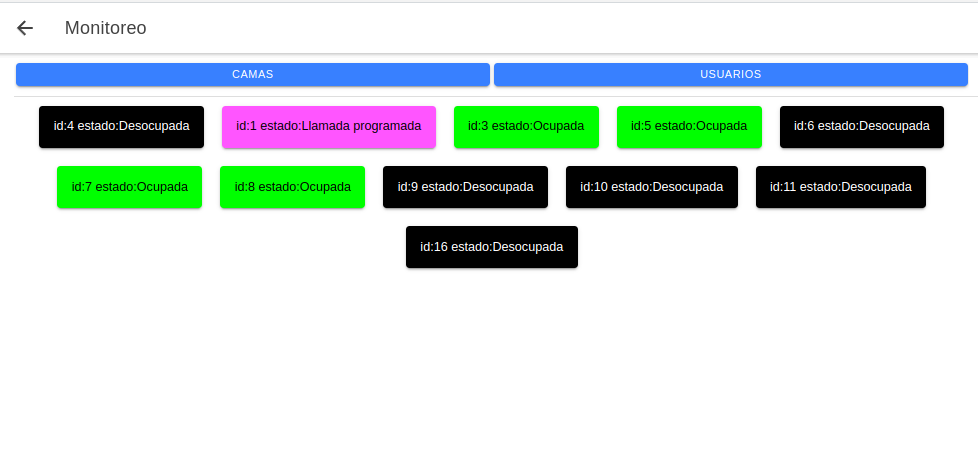
\includegraphics[scale=.55]{./Figures/monitoreo-camas.png}
	\caption{Monitoreo de camas.}
	\label{fig:Monitoreo de camas.}
\end{figure} 

\subsection{Gestión de tareas programadas}

Si se desea generar un nuevo evento programado, se selecciona del menú  calendario, se selecciona el número de paciente y luego se presiona agregar. En ese momento se presenta el formulario de la figura \ref{fig:Tareas programadas.}, se lo completa y se presiona enviar. Los datos a completar son:
\begin{itemize}
\item Nota: campo donde se presenta la tarea propiamente dicha.
\item tipo: se selecciona si es diario, semanal o mensual.
\item en el calendario se selecciona fecha y hora de inicio, desde ese momento se repite segun el tipo.
\end{itemize}

\begin{figure}[ht]
	\centering
	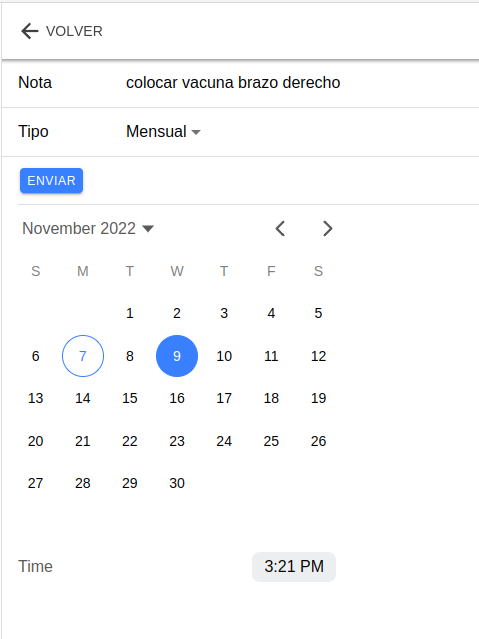
\includegraphics[scale=.40]{./Figures/tarea-programada.png}
	\caption{Tareas programadas.}
	\label{fig:Tareas programadas.}
\end{figure} 

El backend guarda en la base de datos la nueva tarea y genera la acción correspondiente.

\pagebreak
\subsection{Estadísticas del sistema}

En esta sección se puede observar la cantidad de atenciones por enfermero guardadas en la base de datos, la relación entre las distintas especialidades y la relación entre tratamientos y pacientes. En la figura \ref{fig:Relación paciente tratamiento.} se muestra una de las subsecciones que se pueden seleccionar. Para generar las graficas se utiliza HighCharts \citep{WEBSITE:33} (las especialidades son de fantasía, creadas solo para el ejemplo). 
\begin{figure}[ht]
	\centering
	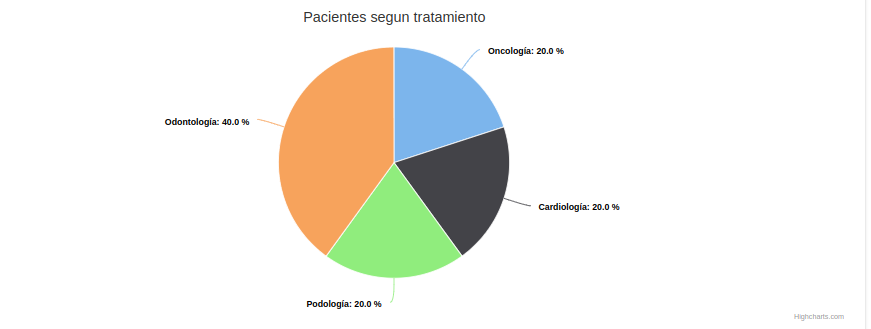
\includegraphics[scale=.65]{./Figures/web/pacientes-Tratamiento.png}
	\caption{Relación paciente tratamiento.}
	\label{fig:Relación paciente tratamiento.}
\end{figure} 


\pagebreak
\section{Aplicación Móvil}
\label{Aplicación Móvil}
En esta sección se presenta la funcionalidad de la aplicación móvil y algunos detalles de la implementación.
\label{Estructura y organización del software}
\subsection{Estructura y organización del software}
La estructura de directorios del proyecto es la presentada en la figura \ref{fig: Estructura de código fuente de la aplicación móvil.}.

\begin{figure}[ht]
	\centering
	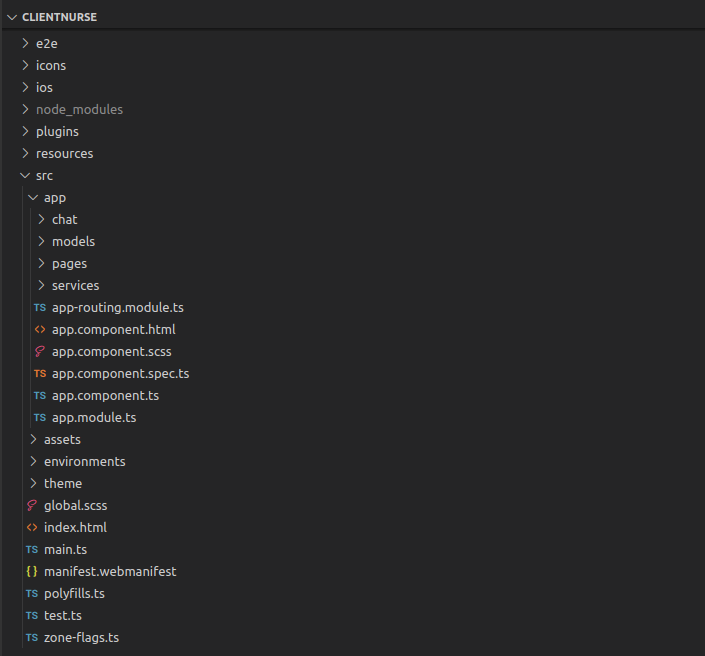
\includegraphics[scale=.60]{./Figures/app/estructura-app.png}
	\caption{ Estructura de carpetas de la aplicación móvil.}
	\label{fig: Estructura de código fuente de la aplicación móvil.}
\end{figure} 

El código de las distintas páginas por las que navega el usuario se encuentra dentro de \textit{''./src/app/pages''}. Los modelos (''clases'') utilizados se encuentra en la carpeta \textit{''./src/app/models''} y los servicios en la carpeta \textit{''./src/app/services''}. La carpeta \textit{''./src/app/chat''} contiene la primera versión la intercomunicación entre enfermeros-médicos que simulaba una sala de reunión  (similar a la ofrecida por el producto en el mercado). Luego se migró a la definitiva, que cumple estrictamente con lo solicitado en un principio, pero por solicitud del cliente, no se eliminó la carpeta.

Como se mencionó en la seccion \ref{Generación del entorno base para el desarrollo del sistema de backend}, la aplicación móvil interactua con el backend solo utilizando websockets MQTT.

La aplicación posee un módulo principal llamado ''app.module''. Utilizando el angular-router, se redirecciona desde cualquier página a una deseada. En el código \ref{cod:Rutas aplicación Móvil.} se presenta como se redireccionan las páginas en Ionic:

\begin{lstlisting}[label=cod:Rutas aplicación Móvil.,caption=  Fragmento de las rutas de la aplicación móvil.]
const routes: Routes = [
  {
    path: 'home',
    loadChildren: () => import('./pages/home/home.module').then( m => m.HomePageModule)
  },
  {
    path: '',
    redirectTo: 'home',
    pathMatch: 'full'
  },
  {
    path: 'mqtt-config',
    loadChildren: () => import('./pages/mqtt-config/mqtt-config.module').then( m => m.MqttConfigPageModule)
  },
  {
    path: 'login',
    loadChildren: () => import('./pages/login/login.module').then( m => m.LoginPageModule)
  },
  ...

\end{lstlisting} 

\pagebreak

\subsection{Configuración del broker y acceso de usuario}

Cuando se inicia la aplicación se presenta una pantalla con dos pulsadores, uno redirige a la página de configuración del broker MQTT y otro a la página de ingreso.
%\begin{figure}[ht]
%	\centering
%	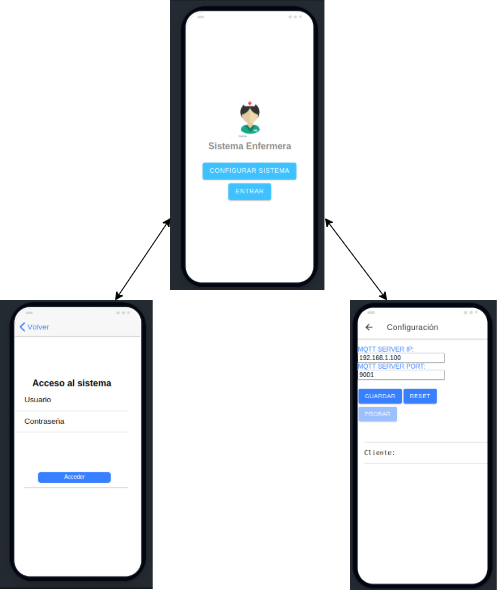
\includegraphics[scale=.80]{./Figures/app/inicioApp.png}
%	\caption{ Pantalla inicial, configuración y acceso de la aplicación.}
%	\label{fig: Pantalla inicial, configuración y acceso de la aplicación.}
%\end{figure} 



\begin{figure}[!htpb]
     \centering
     \begin{subfigure}[b]{0.3\textwidth}
         \centering
         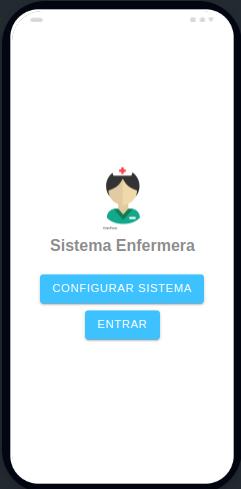
\includegraphics[width=1.1\textwidth]{./Figures/app/main-page.png}
         \caption{Pantalla Inicial.}
         \label{fig_0:1_de_3}
     \end{subfigure}
     \hfill
     \begin{subfigure}[b]{0.3\textwidth}
         \centering
         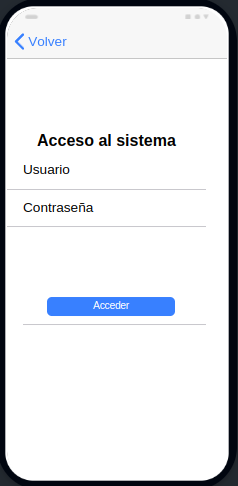
\includegraphics[width=1.1\textwidth]{app/login-page.png}
         \caption{Pantalla login.}
         \label{fig_0:2_de_3}
     \end{subfigure}
     \hfill
     \begin{subfigure}[b]{0.3\textwidth}
         \centering
         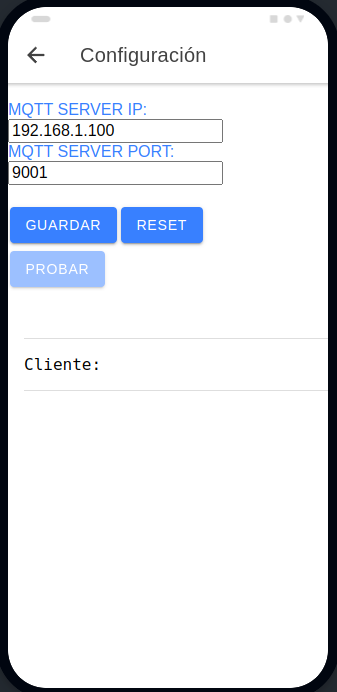
\includegraphics[width=1.1\textwidth]{./Figures/app/system-config.png}
         \caption{Configuración.}
         \label{fig_0:3_de_3}
     \end{subfigure}
        \caption{Inicio de sistema}
        \label{fig:Pantalla inicial, configuración y acceso de la aplicación.}
\end{figure}

En la página de configuración se ingresa la IP del broker del sistema y el puerto. Luego se puede probar la comunicación y guardar los parametros en el localStorage del dispositivo.

\begin{lstlisting}[label=cod:LocalStorage,caption=  Funciones del servicio que guardan en el localStorage.]
  /**
   * Saving port values to localStorage
   */
  public saveValues = async () => {     
    this.localSto.saveValuesString('MQTTSERVER',this.MQTTSERVER);
    this.localSto.saveValuesNumber('MQTTPORT',this.MQTTPORT);
  };
\end{lstlisting}

En la página de logueo se ingresan el nombre de usuario, y su contraseña.

La aplicación publica la información en el tópico ''/User/username'' con el formato de mensaje correspondiente y recibe en ''/Session/nrodesesión'' el número de usuario y el modo de uso. De esta manera la aplicación se setea en el modo correspondiente.



\subsection{Modo administrador}
En el modo administrador se puede monitorear el estado de los usuarios y las camas. Para seleccionar lo que se desea monitorear, se presiona el botón correspondiente.

\begin{figure}[ht]
	\centering
	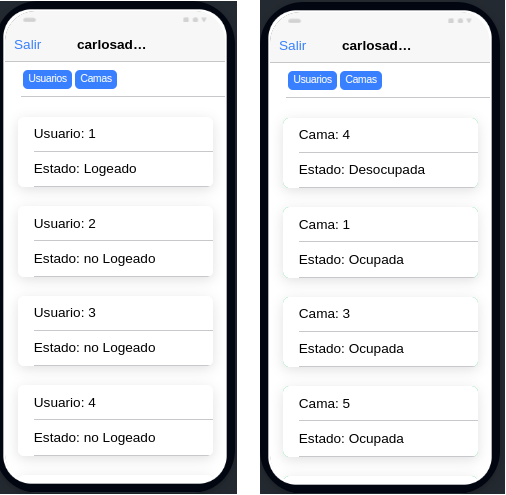
\includegraphics[scale=.70]{./Figures/app/administracion.png}
	\caption{ Pantallas de administración.}
	\label{fig: Pantallas de administración.}
\end{figure} 

El orden en que se presentan las camas tienen que ver con la prioridad que se les asignó a cada una.



\pagebreak
\subsection{Modo médico}
Al ingresar en modo médico, la aplicación queda en modo de espera hasta que el usuario decida que hacer. El diagrama de estados se presenta en la figura \ref{fig: Diagrama de estados en modo médico.}. 

\begin{figure}[ht]
	\centering
	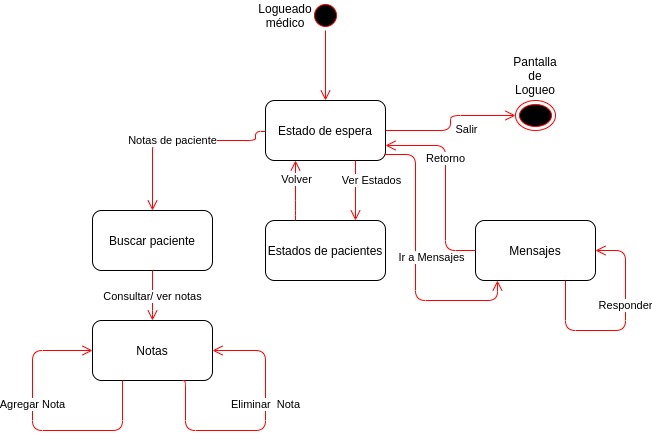
\includegraphics[scale=.65]{./Figures/app/modo-medico.png}
	\caption{ Diagrama de estados en modo médico.}
	\label{fig: Diagrama de estados en modo médico.}
\end{figure} 

Las acciones que puede realizar un médico son:
\begin{itemize}
\item Actualizar una nota de un paciente: para la gestión de estos mensajes se utiliza el tópico ''/Pacient/id'' donde id es el número de paciente. Cuando el médico solicita información del paciente (nombre, apellido y número ) se responde  en ''/Pacient/id/info''. Cuando se consulta las notas se responde en ''/Pacient/id/notes'' y cuando se quiere ingresar una nueva nota se publica en ''/Pacient/id/newNote''
\item Responder a una consulta de una enfermera.
\item Monitorear las camas con los pacientes que le fueron encargados: simplemente filtra por sus pacientes el listado publicado en ''/Beds/status''

\end{itemize}


\begin{figure}[!htpb]
     \centering
     \begin{subfigure}[b]{0.3\textwidth}
         \centering
         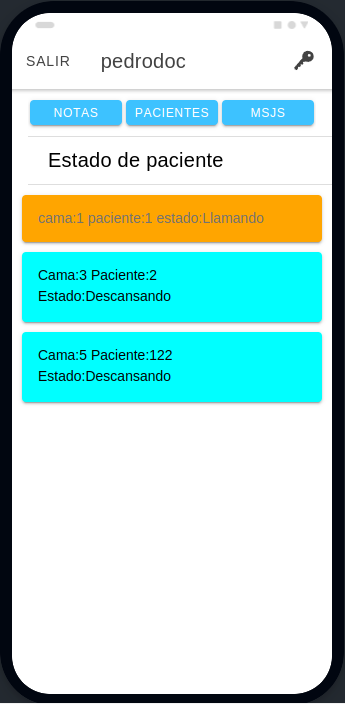
\includegraphics[width=.95\textwidth]{./Figures/app/doctor-patient-1.png}
         \caption{Monitoreo de pacientes.}
         \label{fig_1:1de3}
     \end{subfigure}
     \hfill
     \begin{subfigure}[b]{0.3\textwidth}
         \centering
         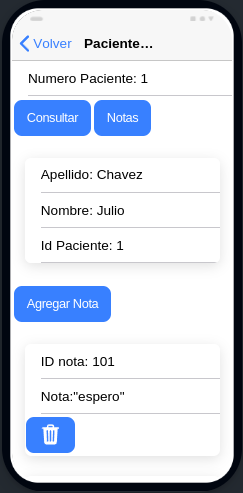
\includegraphics[width=.95\textwidth]{app/doctor-notes5.png}
         \caption{Gestión de notas.}
         \label{fig_1:2de3}
     \end{subfigure}
     \hfill
     \begin{subfigure}[b]{0.3\textwidth}
         \centering
         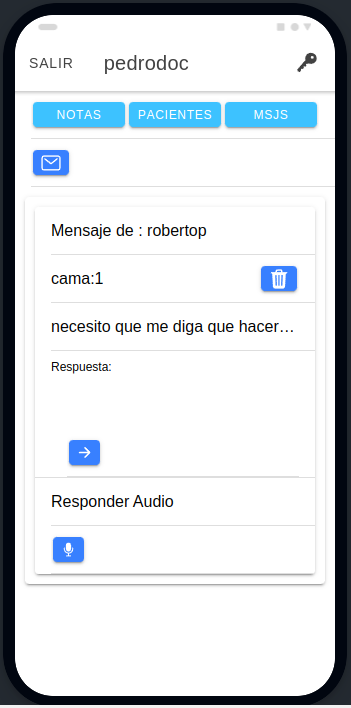
\includegraphics[width=.95\textwidth]{./Figures/app/doctor-message-audio.png}
         \caption{Mensajes.}
         \label{fig_1:3de3}
     \end{subfigure}
        \caption{Modo médico}
        \label{fig:Modo médico}
\end{figure}

\pagebreak
\subsection{Modo enfermera}

Es el modo más complejo por la cantidad de opciones que se pueden presentar.

Al ingresar en modo enfermera, la aplicación consulta al backend por la especialización del enfermero corresponidente y la respuesta se obtiene de escuchar en el tópico ''/User/userId/Specs''donde userId se recibió al loguearse.

Para el usuario, la aplicación queda en modo espera hasta que se reciba una notificación de necesidad de atención. El diagrama de estados se presenta en la figura \ref{fig: Diagrama de estados en modo enfermera.}.

 

La aplicación se encuentra escuchando al tópico MQTT ''/Beds/status'', y filtra los estados (solo acepta estados con llamadas , llamadas programadas o ayuda) y por especialidad del enfermero. De esta manera, cuando un enfermero acepta una tarea, automáticamente se actualiza el backend y ningún otro enfermero puede aceptarla.



\begin{figure}[ht]
	\centering
	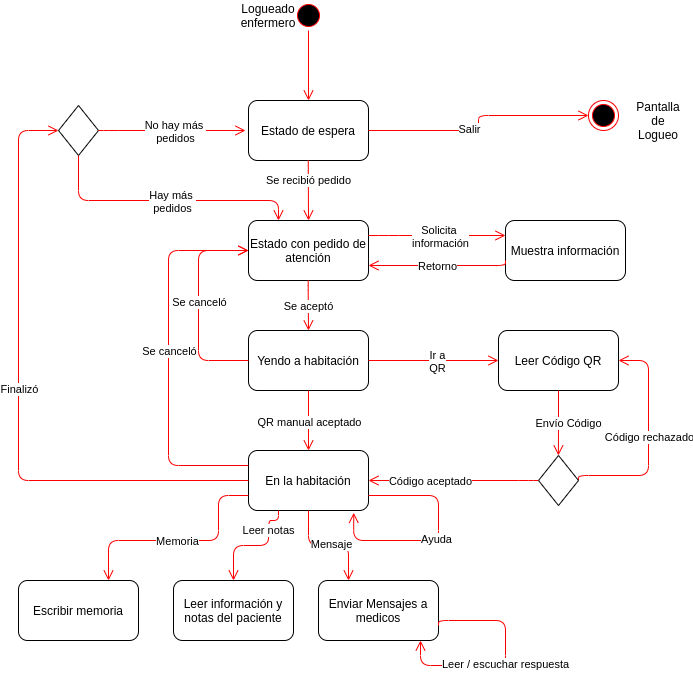
\includegraphics[scale=.60]{./Figures/app/estados-enf.png}
	\caption{ Diagrama de estados en modo enfermera.}
	\label{fig: Diagrama de estados en modo enfermera.}
\end{figure} 



Cuando arriba la notificación, se presenta una tarjeta con dos botones: información de la cama y aceptación. En caso que la enfermera desee consultar donde se encuentra (piso y habitación) debe presionar el boton información. En caso que decida ir a la habitación, debe presionar aceptar.
Al presionar aceptar automáticamente el estado de la cama cambia a desplazandose a la habitación (la información proviene del sistema que recibió la aceptación y cambió el estado de la habitación). Se presentan estas capturas en la figura \ref{fig_2:Recepción de tarea}.

\begin{figure}[!htpb]
     \centering
     \begin{subfigure}[b]{0.3\textwidth}
         \centering
         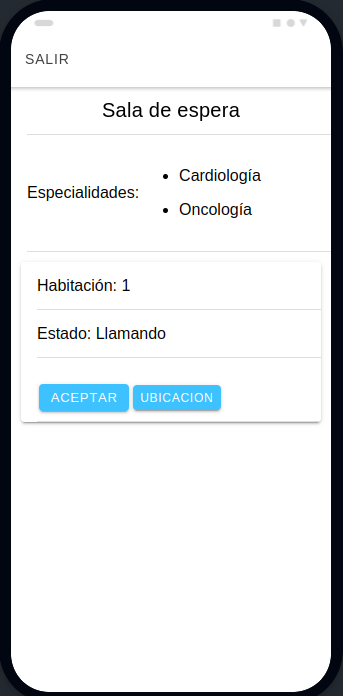
\includegraphics[width=.95\textwidth]{./Figures/app/enfermera-peticion.png}
         \caption{Se recibe peticion.}
         \label{fig_2:1de3}
     \end{subfigure}
     \hfill
     \begin{subfigure}[b]{0.3\textwidth}
         \centering
         \includegraphics[width=.95\textwidth]{app/enfermera-cama.png}
         \caption{Solicita información.}
         \label{fig_2:2de3}
     \end{subfigure}
     \hfill
     \begin{subfigure}[b]{0.3\textwidth}
         \centering
         \includegraphics[width=.95\textwidth]{./Figures/app/yendo-enfermera.png}
         \caption{Tarea aceptada.}
         \label{fig_2:3de3}
     \end{subfigure}
        \caption{Recepción de tarea}
        \label{fig_2:Recepción de tarea}
\end{figure}

Cuando el usuario se encuentra frente al paciente, puede ingresar el código correspondiente a la cama manualmente o bien leer el código QR con el celular, como se observa en la figura \ref{fig: Captura de QR en la aplicación.}.

\begin{figure}[ht]
	\centering
	\includegraphics[scale=.05]{./Figures/app/capturaQR.jpg}
	\caption{ Captura de QR en la aplicación}
	\label{fig: Captura de QR en la aplicación.}
\end{figure} 


Una vez que se aceptó desde el sistema el código de la cama, en la aplicación se presenta una pantalla con distintos botones (ver figuras \ref{fig_3:Ejecución de tarea}). Las acciones que se permiten realizar son:


\begin{enumerate}
\item Cancelar: envía al sistema automáticamente la solicitud de cancelar la tarea. El sistema vuelve a colocar a la cama en situación de llamada.
\item Listo: envía al sistema automáticamente la solicitud de finalizar la tarea. El sistema coloca a la cama en situación de ocupada.
\item Notas: consulta al sistema las notas referidas al paciente. 
\item Mensajes: permite enviar audio o texto a un médico. 
\item Ayuda: solicita al sistema que marque a la cama como con solicitud de ayuda para que otros enfermeros puedan socorrer al usuario. 
\item Memoria: Permite incorporar un texto que se almacena junto con la tarea al presionar Listo.
\end{enumerate}

\begin{figure}[!htpb]
     \centering
     \begin{subfigure}[b]{0.3\textwidth}
         \centering
         \includegraphics[width=.95\textwidth]{./Figures/app/enfermera-trabajando.png}
         \caption{Menu dentro de habitación.}
         \label{fig_3:1de3}
     \end{subfigure}
     \hfill
     \begin{subfigure}[b]{0.3\textwidth}
         \centering
         \includegraphics[width=.95\textwidth]{app/enfermera-consultaNotas.png}
         \caption{Solicita información y notas.}
         \label{fig_3:2de3}
     \end{subfigure}
     \hfill
     \begin{subfigure}[b]{0.3\textwidth}
         \centering
         \includegraphics[width=.95\textwidth]{./Figures/app/enfermera-msg.png}
         \caption{Abriendo menú de mensajes.}
         \label{fig_3:3de3}
     \end{subfigure}
        \caption{Ejecución de tarea}
        \label{fig_3:Ejecución de tarea}
\end{figure}

%	% Chapter Template

\chapter{Ensayos y resultados} % Main chapter title

En este capítulo se describen los ensayos realizados, se comentan las herramientas que se utilizaron y se presentan los resultados. Se fragmenta el capítulo en dos partes : pruebas unitarias e integración del sistema.

\label{Chapter4} % Change X to a consecutive number; for referencing this chapter elsewhere, use \ref{ChapterX}

%----------------------------------------------------------------------------------------
%	SECTION 1
%----------------------------------------------------------------------------------------


\section{Pruebas unitarias}
En esta sección se presentan las herramientas que se utilizaron para ensayar las distintas partes del sistema en forma separada.

\subsection{Pruebas del servidor Mosquitto}
Para simular mensajes y observar el comportamiento de cada una de las partes del sistema se utilizó la herramienta MQTT explorer   \citep{WEBSITE:29} que se presenta en la figura \ref{fig:MQTT Explorer}.

\begin{figure}[ht]
	\centering
	\includegraphics[scale=.30]{./Figures/mqtt-explorer.png}
	\caption{Imagen de MQTT Explorer.}
	\label{fig:MQTT Explorer}
\end{figure}

Esta herramienta fue importante no solo para realizar ensayos sino también para el desarrollo de las funcionalidades propiamente dichas.

\pagebreak

\subsection{Pruebas unitarias de la API Rest}

Para simular el logeo y la consulta a la base de datos se utilizó la herramienta PostMan \citep{WEBSITE:30}, Newman \citep{WEBSITE:35} y la consola de administrador de phpMyAdmin mencionada en \ref{subsec: Bases de datos relacionales}. En la figura \ref{fig:Logueo en el sistema con Postman} se observa el \textit{token} devuelto por el backend al loguearse con las credenciales correspondientes y en \ref{fig:Rechazo Logueo en el sistema con Postman} se observa la respuesta al ingresar una contraseña inadecuada.


En esta secuencia, el cliente (en este caso Postman), envía en el body el nombre de usuario (''username'') y la contraseña (''password'') en formato JSON. Según lo explicado en la sección  \ref{Descripción de API Rest para aplicación Web}, el backend realiza ciertas verificaciones y devuelve un token de sesión en el body.

\begin{figure}[ht]
	\centering
	\includegraphics[scale=.35]{./Figures/auth.png}
	\caption{Logueo en el sistema con Postman.}
	\label{fig:Logueo en el sistema con Postman}
\end{figure}

\begin{figure}[ht]
	\centering
	\includegraphics[scale=.35]{./Figures/no-auth.png}
	\caption{Rechazo de logueo.}
	\label{fig:Rechazo Logueo en el sistema con Postman}
\end{figure}

Postman permite automatizar los test utilizando colecciones (que son secuencias de consultas a la API). Las colecciones se pueden exportar a un formato JSON de modo de poder ser utilizadas por otras herramientas. 

En un entorno de integración continua y entrega continua, una herramienta de testeo automático permite, una vez definidas las colecciones de test, volver a ejecutarlas luego de haber realizado una modificación,  asegurar que no se modificó lo que ya funcionaba y que las mejoras pasan los nuevos test. La ventaja de utilizar newman radica en que al tener un cliente de consola se puede generar un script automático.

Para utilizar Newman, que es el cliente de consola, se deben exportar las colecciones y luego utilizar la línea de comandos con dicha colección (ver figura \ref{fig:Colección logueo usuario en Postman}). Existen varias opciones de reportes de resultados, en este trabajo se utiliza cli y htmlextra, ejecutando en la consola el código \ref{cod:Newman}.

\begin{figure}[ht]
	\centering
	\includegraphics[scale=.35]{./Figures/Postman.png}
	\caption{Colección test de logueo.}
	\label{fig:Colección logueo usuario en Postman}
\end{figure}

\begin{lstlisting}[label=cod:Newman,caption=  Ejecución de Newman en consola.]
>>newman run ./logueo_usuario.postman_collection.json -r cli,htmlextra
\end{lstlisting}

En la figura \ref{fig:reporte cli Newman} se observa el reporte por consola.
\begin{figure}[ht]
	\centering
	\includegraphics[scale=.50]{./Figures/newman-1.png}
	\caption{Reporte en consola de Newman.}
	\label{fig:reporte cli Newman}
\end{figure}




\pagebreak

\section{Integración del sistema}
\label{Integración del sistema}

En esta sección se explica como se instaló el backend y el servidor web en una máquina remota, se instaló la aplicación en múltiples dispositivos, se desarrolló un dispositivo que simula los eventos de los llamadores de los hospitales, se ensayó el sistema durante una semana.  Finalmente se analizan los resultados de la simulación de uso.

Se utilizó como máquina remota una instancia en Amazon Web Services. Los dispositivos móviles en los cuales se instaló la aplicación poseían el sistema Android como sistema operativo.

\subsection{Instalación del sistema en una instancia de AWS}
Con el objetivo de no incorporar costos en las pruebas, se generó una instancia Free Tier en Amazon Web Services, en la cual se instaló Ubuntu, el broker Mosquitto, el backend, la página Web y un servidor NGINX para que funcione como proxy reverso. También se contrató el servicio route 53 que permite personalizar las políticas de ruteo.
De esta manera, se puede acceder al sistema desde cualquier dispositivo móvil conectado a una red.
Los pasos para configurar el sistema backend en la instancia EC2 con ubuntu son:
\pagebreak

\begin{enumerate}


\item Loguearse en la instancia con ssh.
\item Setear la base temporal en Buenos Aires Argentina (esto es importante \\ ya que hay eventos de calendario que se deben realizar en el tiempo correspondiente a este huso horario). Esto se presenta en el código \ref{cod:Set DateTime}.\\

\begin{lstlisting}[label=cod:Set DateTime,caption=  Configuración de zona horaria.]
	sudo echo "America/Argentina/Buenos_Aires" | sudo tee /etc/timezone
	sudo dpkg-reconfigure --frontend noninteractive tzdata
	sudo reboot
\end{lstlisting}

\item Instalar Git:

	sudo apt-get install git
\item Instalar el broker Mosquitto:
	
	sudo apt-get install mosquitto
\item Configurar el brocker Mosquitto según la sección \ref{Broker Mosquitto}.
\item Instalar Docker y Docker-compose según el sitio \citep{WEBSITE:8}
\item Descargar el backend desde GitHub:

	git clone  https://github.com/gustavobastian/ServerNurse
\item Copiar en la instancia la base de datos (utilizar el protocolo SCP) comprimida y descomprimir dentro de la carpeta /db
\pagebreak
\item Crear el archivo de entorno (.env) según el código \ref{cod:Entorno_backend}:


\begin{lstlisting}[label=cod:Entorno_backend,caption=  Entorno del backend.]
TAG="v1.0.1"

##SECURITY
#secret pass
JWT_SECRET = <palabra secreta para las contrasenas>
#token expiration time
JWT_EXP_TIM = 120s


##MQTT CONFIGURATION
##setting por for using websockets
MQTT_CONNECTION = 'ws://<IP de broker>:<puerto de broker>'

##server
PORT_LOCAL    = 3000

##timezone

TZ = America/Argentina/Buenos_Aires 
\end{lstlisting}


\item Ejecutar Docker-compose up
\end{enumerate}

Los pasos para configurar la página web son:
\begin{itemize}
\item Compilar la página web: para ello, dentro del proyecto ejecutar:

''ionic build --prod''
\item Comprimir la carpeta www.
\item Loguearse con ssh en la instancia EC2.
\item Copiar el archivo comprimido en la instancia y descomprimirlo en ''/var/www/hmtl''.
\item Configurar nginx para redirigir a la página (ver apéndice \ref{AppendixB}).

\end{itemize}

\subsection{Generación/instalación de la aplicación móvil en Android}

Para que la aplicación pueda utilizarse en un dispositivo móvil, la misma debe ser compilada para ejecutarse en código nativo. Con esto se genera el código instalable .apk para Android y .ipa para IOS. 

Para poder descargar el archivo ejecutable a un dispositivo Android se debe generar el archivo .apk correspondiente. Para ello se deben ejecutar los siguientes pasos:

\begin{enumerate}

\item Generar el código con ionic capacitor:
''ionic cap build android''
\item Abrir Android Studio (ver apéndice \ref{AppendixC}).
\item Generar el bundle o en su defecto, conectar el celular en modo debug y descargar la aplicación. 
\end{enumerate}
\pagebreak


\subsection{Equipo simulador de llamadores}

Se desarrolló un dispositivo que simula los llamadores con un microcontrolador ESP32, una fuente y un teclado matricial. Presionando una tecla, se genera un evento en MQTT. El código y el esquemático del mismo se encuentra en \citep{WEBSITE:33} y se presentan algunos detalles del código en el anexo \ref{AppendixA}. Es importante mencionar que el dispositivo desarrollado posee la funcionalidad mínima, pero permite simular múltiples habitaciones (no fue pensado para un uso real).

\begin{figure}[ht]
	\centering
	\includegraphics[scale=.35]{./Figures/simulador.png}
	\caption{Simulador de llamadores.}
	\label{fig:Simulador de llamadores}
\end{figure}

\subsection{Resultados de las pruebas de integración}
\label{Resultados de las pruebas de integración}
El sistema permaneció funcionando de manera adecuada durante una semana completa, generando los eventos programados y permitiendo la interacción de dispositivos.

\pagebreak
\section{Contraste con los requerimientos}
\label{Contraste con los requerimientos}

En esta subsección se detalla el grado de cumplimiento de los requerimientos relevados en el plan de proyecto.
\begin{enumerate}
\item Requerimientos del servidor: 

1.1 debe tener instalado el broker mosquitto.

Verificación: Se muestra el funcionamiento del servidor utilizando la aplicación MQTT explorer.

\item Requerimientos de la base de datos: 

2.1 Debe poseer una base de datos relacional. 

2.2 Debe poseer las siguientes tablas: eventos, pacientes, médicos, enfermeras. 

2.2 La base de datos debe poseer datos cargados por default.

Verificación: Se muestra el contenido de la base de datos con la aplicación phpMyAdmin.

\item Requerimientos de la página web 

3.1 Debe ser cliente del broker MQTT. 

Verificación: Se presenta la configuración del broker. Se presenta el monitoreo de las habitaciones y los usuarios conectándose al broker.

3.2 La página debe poseer funciones de consulta o modificación de la base de datos.

Verificación: Se muestra como la página web permite cambiar contraseñas de usuarios y otros parámetros.

3.3 La página debe permitir observar la estadística de pacientes y enfermeras.

Verificación: Se muestra como la página web permite observar distintas gráficas.

3.4 La página debe contener acceso con usuario y contraseña para cada persona.


Verificación: Se muestra como la página web permite loguear los distintos usuarios.
 
(*) Cumplimiento parcial: solo permite loguear al usuario administrador.

\item Requerimientos de la aplicación móvil

4.1 y 4.2 La aplicación debe poseer tres modos de uso: médico, enfermera y sistema. 

Verificación: Se ingresa a la aplicación en los distintos modos.

4.3 La aplicación en modo enfermera debe permitir leer código QR.

Verificación: Se ingresa a la aplicación en modo enfermera y siguiendo los pasos se obtiene el código QR.

4.4 La aplicación en modo enfermera debe descargar información relevante del paciente.

Verificación: Se ingresa a la aplicación en modo enfermera y siguiendo los pasos se descarga las notas del paciente.

4.5 La aplicación en modo sistema debe mostrar las habitaciones sin atención, según una tabla de prioridades y en caso de igualdad de prioridades mostrar según un orden de llamada.

(*) Cumplimiento parcial: se muestra las habitaciones con una tabla de prioridades pero no según el orden de llamadas.

Verificación: Se ingresa a la aplicación en modo enfermera y siguiendo los pasos se descarga las notas del paciente.


4.6 El modo de usuario médico y el modo usuario enfermera deben poder enviar mensajes de texto o sonido.

Verificación: Se transmiten distintos audios entre participantes.

\item Requerimientos de la documentación

5.1 Documento con información relativa a la base de datos: detalles de la misma y API para acceder.

Verificación: Se observa la presencia de la información en el repositorio de GitHub.

5.2 Memoria del proyecto con diagramas de aplicación móvil y página web.

Verificación: se verifica con este documento.

\item Requerimientos de la integración del sistema

6.1 El sistema debe integrar el funcionamiento del servidor con la base de datos, aplicación web y aplicaciones móviles.

Verificación: se verificó el funcionamiento en un laboratorio con 4 usuarios y un simulador de 8 llamadores durante una semana.

(*) Cumplimiento parcial:
Validación: No se pudo validar el sistema en un nosocomio.

\item Requerimientos de la entrega del producto:

7.1 El Código fuente del servidor debe ser subido a dockerhub y compartido con la comunidad.

(*) Cumplimiento parcial:
Validación: Se subió el código fuente del servidor a GitHub.

7.2 El Código fuente de la aplicación debe ser subido a GitHub y compartido con la comunidad.

Validación: Se subió el código fuente del servidor a Github.

\end{enumerate}
 
%	% Chapter Template

\chapter{Conclusiones} % Main chapter title

\label{Chapter5} % Change X to a consecutive number; for referencing this chapter elsewhere, use \ref{ChapterX}


%----------------------------------------------------------------------------------------

%----------------------------------------------------------------------------------------
%	SECTION 1
%----------------------------------------------------------------------------------------

\section{Notas sobre el sistema desarrollado }

%La idea de esta sección es resaltar cuáles son los principales aportes del trabajo realizado y cómo se podría continuar. Debe ser especialmente breve y concisa. Es buena idea usar un listado para enumerar los logros obtenidos.

%Algunas preguntas que pueden servir para completar este capítulo:

%\begin{itemize}
%\item ¿Cuál es el grado de cumplimiento de los requerimientos?
%\end{itemize}
%\item ¿Cuán fielmente se puedo seguir la planificación original (cronograma incluido)?
%\item ¿Se manifestó algunos de los riesgos identificados en la planificación? ¿Fue efectivo el plan de mitigación? ¿Se debió aplicar alguna otra acción no contemplada previamente?
%\item Si se debieron hacer modificaciones a lo planificado ¿Cuáles fueron las causas y los efectos?
%\item ¿Qué técnicas resultaron útiles para el desarrollo del proyecto y cuáles no tanto?
%\end{itemize}
En este capítulo se analiza el proyecto en su totalidad , el trabajo realizado y los pasos a seguir.



El principal aporte que presenta el proyecto consiste en el modelo que se propuso para el sistema de backend, con dos APIs totalmente separadas para interactuar con la base de datos. De esta manera, si se quiere escalar el proyecto , se pueden agregar funcionalidades de manera independiente a la página de administración y a la aplicación móvil. Otro aporte importante es el uso de MQTT para una aplicación de estas características con el modelo de subcripción a tópicos.

Se pudo lograr cumplir con los requerimientos en un porcentaje alto. 

\subsection{Cumplimiento de planificación original}

No se pudo seguir con la planificación original ya que se presentaron situaciones no contempladas en la misma. Se enumeran a continuación:
\begin{enumerate}
\item Agregado de funcionalidades necesarias pero no contempladas en un inicio.
\item Configuración de los dispositivos para la aplicación.

\end{enumerate}


\subsection{Gestión de riesgos}

El principal riesgo que se previó era la imposibilidad de desarrollar la aplicación para dispositivos IOS debido a la ausencia de un equipo en el cual desarrollar y otro para testear. Efectivamente se cumplió y no se pudo llegar a satisfacer ese requerimiento.

\subsection{Recursos aprendidos durante la carrera:}
En el desarrollo del trabajo se utilizaron las siguientes herramientas presentadas durante el trayecto de la carrera:

\begin{itemize}
\item Gestión de proyectos: se elaboró un plan de trabajo y el relevamiento de requerimientos.
\item Protocolos de Internet, Protocolos de IoT y Diseño de aplicaciones para IOT: se utilizaron los conceptos aprendidos sobre MQTT en estas materias.
\item Arquitectura de datos: se utilizó los conceptos sobre bases de datos enseñados en esta asignatura.
\item Ciberseguridad en Internet de las Cosas: se utilizaron los conceptos sobre seguridad enseñados en esta materia, principalmente en la página web de configuración.
\item Testing de sistemas de IoT: se utilizó la tecnica de testing del backend utilizando Postman enseñada en esta materia.
\item Diseño de páginas Web, Diseño de aplicaciones multiplataformas y Diseño de aplicaciones para Iot: se utilizaron los frameworks, las técnicas y los lenguajes de programación enseñados en estas materias.
\end{itemize}

%----------------------------------------------------------------------------------------
%	SECTION 2
%----------------------------------------------------------------------------------------
\section{Proximos pasos}

%Acá se indica cómo se podría continuar el trabajo más adelante.

Este trabajo sirve de base para la implementación de un sistema de gestión hospitalaria general. Los items que se pueden mejorar son:

\begin{itemize}
\item Generar el código para que la aplicación corra en IOS.
\item Utilizar una base de dato clave-valor para reemplazar la lista de usuarios en el monitoredo del backend.
\item Mejorar la seguridad utilizando TLS en el broker Mosquitto (por una razón de tiempo no se pudo desarrollar).
\item En el logeo de eventos se guardan números de referencia de usuario que realizó la acción y número de paciente. Se puede utilizar otra identificación suplementaria como ser nombre y apellido.
\item La estadística que se consulta a la base de datos es mínima. Se puede analizar otras cosas como ser duración promedio, pacientes con mayor tiempo de atención, etc.
\item Desarrollar un dispositivo llamador que se pueda utilizar en ámbitos hospitalarios.

\end{itemize}
 
%\end{verbatim}

%Los apéndices también deben escribirse en archivos .tex separados, que se deben ubicar dentro de la carpeta \emph{Appendices}. Los apéndices vienen comentados por defecto con el caracter \code{\%} y para incluirlos simplemente se debe eliminar dicho caracter.

%Finalmente, se encuentra el código para incluir la bibliografía en el documento final.  Este código tampoco debe modificarse. La metodología para trabajar las referencias bibliográficas se desarrolla en la sección \ref{sec:biblio}.
%----------------------------------------------------------------------------------------

%\section{Bibliografía}
%\label{sec:biblio}

%Las opciones de formato de la bibliografía se controlan a través del paquete de latex \option{biblatex} que se incluye en la memoria en el archivo memoria.tex.  Estas opciones determinan cómo se generan las citas bibliográficas en el cuerpo del documento y cómo se genera la bibliografía al final de la memoria.

%En el preámbulo se puede encontrar el código que incluye el paquete biblatex, que no requiere ninguna modificación del usuario de la plantilla, y que contiene las siguientes opciones:

%\begin{lstlisting}
%\usepackage[backend=bibtex,
%	natbib=true, 
%	style=numeric, 
%	sorting=none]
%{biblatex}
%\end{lstlisting}

%En el archivo \file{reference.bib} se encuentran las referencias bibliográficas que se pueden citar en el documento.  Para incorporar una nueva cita al documento lo primero es agregarla en este archivo con todos los campos necesario.  Todas las entradas bibliográficas comienzan con $@$ y una palabra que define el formato de la entrada.  Para cada formato existen campos obligatorios que deben completarse. No importa el orden en que las entradas estén definidas en el archivo .bib.  Tampoco es importante el orden en que estén definidos los campos de una entrada bibliográfica. A continuación se muestran algunos ejemplos:

%\begin{lstlisting}
%@ARTICLE{ARTICLE:1,
%    AUTHOR="John Doe",
%    TITLE="Title",
%    JOURNAL="Journal",
%    YEAR="2017",
%}
%\end{lstlisting}


%\begin{lstlisting}
%@BOOK{BOOK:1,
%    AUTHOR="John Doe",
%    TITLE="The Book without Title",
%    PUBLISHER="Dummy Publisher",
%    YEAR="2100",
%}
%\end{lstlisting}


%\begin{lstlisting}
%@INBOOK{BOOK:2,
%    AUTHOR="John Doe",
%    TITLE="The Book without Title",
%    PUBLISHER="Dummy Publisher",
%    YEAR="2100",
%    PAGES="100-200",
%}
%\end{lstlisting}


%\begin{lstlisting}
%@MISC{WEBSITE:1,
%    HOWPUBLISHED = "\url{http://example.com}",
%    AUTHOR = "Intel",
%    TITLE = "Example Website",
%    MONTH = "12",
%    YEAR = "1988",
%    URLDATE = {2012-11-26}
%}
%\end{lstlisting}

%Se debe notar que los nombres \emph{ARTICLE:1}, \emph{BOOK:1}, \emph{BOOK:2} y \emph{WEBSITE:1} son nombres de fantasía que le sirve al autor del documento para identificar la entrada. En este sentido, se podrían reemplazar por cualquier otro nombre.  Tampoco es necesario poner : seguido de un número, en los ejemplos sólo se incluye como un posible estilo para identificar las entradas.

%La entradas se citan en el documento con el comando: 

%\begin{verbatim}
%\citep{nombre_de_la_entrada}
%\end{verbatim}

%Y cuando se usan, se muestran así: \citep{ARTICLE:1}, \citep{BOOK:1}, \citep{BOOK:2}, \citep{WEBSITE:1}.  Notar cómo se conforma la sección Bibliografía al final del documento. 


%	\chapter{Introducción específica} % Main chapter title

\label{Chapter2}

%----------------------------------------------------------------------------------------
%	SECTION 1
%----------------------------------------------------------------------------------------
%Todos los capítulos deben comenzar con un breve párrafo introductorio que indique cuál es el contenido que se encontrará al leerlo.  La redacción sobre el contenido de la memoria debe hacerse en presente y todo lo referido al proyecto en pasado, siempre de modo impersonal.
En este capítulo se presentan las bases teóricas que sustentan el trabajo realizado. Se describen distintas soluciones a cada una de las partes del sistema.

\section{Descripción de tecnologías web para IoT}
\label{sec:Descripción de tecnologías web para IoT}


Los sistemas web utilizan (en su mayoría) una arquitectura cliente/servidor en donde se subdivide las tareas a desarrollar en dos partes. El cliente solicita una acción y el servidor la ejecuta. Las acciones pueden ser obtener información para mostrar en una pantalla, modificar un valor en una base de datos, obtener información para reproducir un sonido o un video, etc. En la programación web, se suele dividir el modelo en 2 partes: \textit{ backend} y \textit{frontend} .  

\subsection{ Breve introduccion a tecnologías de backend}
El \textit{backend}  generalmente se encarga de almacenar y gestionar la información \citep{ARTICLE:4}. En el contexto de este trabajo, el \textit{backend} se comunica con los clientes utilizando 2 protocolos: \textit{Message Queuing Telemetry Transport} (en adelante MQTT )  y HTTP. El primero se utilizó para interactuar con los clientes móviles y el segundo se utilizó para brindar los servicios a la página web de configuración.

El protocolo MQTT \citep{ WEBSITE:5} se ha probado como un protocolo confiable, altamente eficiente y ampliamente utilizado en sistemas IoT \citep{ARTICLE:2}.

MQTT es un protocolo open source simple, liviano y orientado a dispositivos con pocos recursos y baja velocidad de transmisión. Está basado en la pila TCP/IP(del ingles \textit{Transmission Control Protocol/Internet Protocol}, Protocolo de control de transmisión /Protocolo de Internet ), se implementa en la capa de aplicación y utiliza mensajeria bajo el patrón de publicación/subscripción. Las ventajas que provee es la posibilidad de agregar accesorios rápidamente con bajo costo de software, hardware e implementación \citep{ARTICLE:2}.

En la referencia \citep{ARTICLE:2} se realiza un estudio en profundidad del desempeño de varios protocolos de IoT: MQTT, CoAP (\textit{Constrained Application Protocol, Protocolo de Aplicaciones Restringido}), AMQP(\textit{Advanced Message Queuing Protocol}, Protocolo de Encolamiento de Mensajes Avanzado ) y HTTP (\textit{Hypertext Transfer Protocol}, Protocolo de Transferencia de Hipertexto). Se menciona que MQTT es ampliamente utilizado pero muy poco estandarizado en comparación con los demas, y se resalta el hecho que tiene limitaciones en lo referido a seguridad.

En las subcciones \ref{sec: Introducción a las bases de datos},\ref{sec:Docker},\ref{subsec:Docker-compose},\ref{subsec: Node} se explicará el funcionamiento del backend.
\subsection{Breve introduccion a tecnologías frontend}
El \textit{frontend} es la parte del programa o del dispositivo con la que interactua el usuario. Son tecnologías que se ejecutan en un navegador o en una aplicación de telefono celular (también llamado telefono inteligente, o \textit{smartphone}). El equipo que desarrolla el \textit{frontend} consiste en programadores diseñadores UX/UI (del ingles \textit{User Experience / User Iterface}, Experiencia de Usuario/Interfaz de Usuario) y diseñadores gráficos. Las más conocidas tecnologías que se utilizan son: el lenguaje de programación Javascript, HTML (\textit{HyperText Markup Language}, Lenguaje de Marcas de Hipertexto) y CSS (\textit{Cascading Style Sheets}, Hojas de Estilo en Cascada) \citep{ARTICLE:4}. Si se desea profundizar en estas tecnologías, existen muchos sitios web donde se ofrecen referencias de las mismas (ver, por ejemplo: \citep{WEBSITE:13}).  

En los últimos años, se busca facilitar el diseño de  \textit{frontend} mediante librerías como React \citep{WEBSITE:14},  JQuery \citep{WEBSITE:17} o Frameworks como ser Vue \citep{WEBSITE:15}, Angular \citep{WEBSITE:16}, Ionic \citep{WEBSITE:18}. En este trabajo se seleccionó la combinación Ionic/Angular para el desarrollo de la página Web y de la aplicación móvil. En la sección \ref{subsec: Ionic}, se presenta una breve introducción.

\section{Componentes del sistema}
\label{sec:Sistema General}

Al sistema desarrollado se lo puede descomponer en seis partes definidas:

\begin{itemize}
\item  Broker MQTT: servidor encargado de gestionar los mensajes.
\item  Base de datos: almacena información relevante de los pacientes, usuarios y sistema.
\item  Servidor de base de datos: proporciona una API (\textit{Application Programming Interface}, interfaz de programación de aplicaciones) del tipo REST (\textit{representational state transfer}, transferencia de estado representacional) que permite la modificación/consulta de la base de datos desde un dispositivo web. La API provee \textit{endpoints}(puntos de acceso en español) que permiten realizar distintas operaciones como ser carga, consulta, alteración o eliminación de información.
\item  Servidor web/ página web: entrega información a un browser para que pueda mostrar una página web de administración del sistema y de carga de la base de datos.
\item  Sistema: recibe los mensajes MQTT y responde/actúa acorde a las peticiones.
\item Cliente browser: muestra en la pantalla de una computadora o dispositivo la página web de administración.
\item Cliente teléfono: permite a médicos y enfermeras interactuar con el sistema.
\end{itemize}

Como se puede observar, se trata de un sistema distribuido y sus partes pueden estar ubicadas en distintas localidades.

Con el objetivo de facilitar el desarrollo se utilizó un sistema de contenedores que permite correr tres de las 6 partes: la base de datos, el servidor de base de datos y el sistema propiamente dicho. Además  agrupó los subsistemas que modifican la base de datos en una sola aplicación que provee ambos servicios: el sistema y el servidor REST. En la figura  \ref{fig:División del sistema} se presenta un esquema general según esta división.


\begin{figure}[ht]
	\centering
	\includegraphics[scale=.45]{./Figures/DiagramaSistemaOrganizado.png}
	\caption{División del sistema.}
	\label{fig:División del sistema}
\end{figure}



\pagebreak

\section{Descripción del protocolo MQTT}
\label{sec:Descripción del protocolo MQTT}

MQTT fue introducido en 1999 por IBM y Eurotech. Es un protocolo de mensajería por suscripción/publicación especialmente diseñado para la comunicación M2M(\textit{Machine to Machine}, Máquina a Máquina) en dispositivos con bajos recursos \citep{WEBSITE:5} .

Para poder explicar el funcionamiento del protocolo es necesario incorporar conceptos definidos en la especificación \citep{WEBSITE:5}:

\begin{itemize}
\item Mensaje: datos transmitidos mediante el protocolo MQTT  a través de la red por la aplicación. Cuando un mensaje es transmitido, el mismo contiene datos útiles(\textit{"payload"}), un campo que identifica la Calidad de Servicio (\textit{Quality of Service}, QoS), ciertas propiedades y un nombre de tópico.
\item Cliente: programa o dispositivo que utiliza MQTT.
\item Servidor o Broker: programa o dispositivo que actúa como intermediario entre clientes que publican mensajes y clientes que han realizado suscripciones.
\item Sesión: una interacción entre cliente y servidor con estados bien definidos.
\item suscripción: una  suscripción implica un filtrado de tópicos y una máxima calidad de servicio. Una suscripción está asociada a una sola sesión y una sesión puede poseer varias suscripciones.
\item Nombre de tópico: etiqueta que se adjunta a un mensaje la cual es comparada con las suscripciones conocidas en el servidor.
\item Filtro de tópico: es una expresión contenida dentro de la suscripción para indicar interés, por parte del cliente, en uno o más tópicos.
\item Suscripción con comodín o \textit{Wildcard} : es una expresión contenida dentro de la suscripción que contiene un carácter especial o comodín, como ser '+' o '\# ', que representan un nivel único y nivel múltiple respectivamente.

\end{itemize}

En este protocolo, el funcionamiento es el siguiente: 

Al iniciar la conexión, el cliente envía un mensaje CONNECT al broker y este contesta con un CONNECTACK y un código de estado. El broker mantiene abierta la conexión hasta que el cliente envía un comando de desconexión o la conexión se pierde por algún motivo. Los puertos estándar son 1883 para comunicación no encriptada y 8883 para comunicación encriptada utilizando TLS/SSL \citep{ARTICLE:4}.

Luego el cliente MQTT publica mensajes en un broker MQTT, los cuales son recibidos por los clientes suscriptos o bien retenidos para una futura suscripción \citep{WEBSITE:5}. En la figura \ref{fig:Sistema MQTT} se presentan todos los componentes de una red MQTT:  

\begin{figure}[ht]
	\centering
	\includegraphics[scale=.45]{./Figures/MQTT-minimal.png}
	\caption{Esquema de un sistema MQTT.}
	\label{fig:Sistema MQTT}
\end{figure}

La conexión MQTT siempre es entre cliente y broker, nunca entre clientes directamente.


Cada mensaje es publicado en una dirección conocida como "tópico". Los clientes pueden subscribirse a múltiples tópicos y recibir todos los mensajes publicados en cada tópico. MQTT es un protocolo binario y normalmente requiere un encabezado fijo de dos \textit{bytes} y un dato útil (\textit{"payload"}) de hasta 256 MB \citep{ARTICLE:2} . 

Ejemplos de tópicos:

\begin{itemize}
\item  1: /user/1/question
\item  2: /user/1/\#
\item  3: /user/+/question
%\item Capítulo 2: Introducción específica
%\item Capítulo 3: Diseño e implementación
%\item Capítulo 4: Ensayos y resultados
%\item Capítulo 5: Conclusiones
\end{itemize}

En el ejemplo 1, en caso de suscribirse a ese tópico, el cliente recibirá todos los mensajes publicados en el subtópico "question".
En el ejemplo 2, el cliente recibirá todos los mensajes dirigidos al usuario 1.
En el ejemplo 3, el cliente que se suscriba a ese tópico recibirá los mensajes enviados a "question" independientemente del número de usuario.


Utiliza usualmente TCP/IP como protocolo de transporte y puede implementar TLS/SLL para seguridad. Por lo que el servicio cliente-broker es del tipo orientado a la conexión. También puede utilizar otros protocolos de red con soporte bidireccional y sin pérdidas de datos \citep{ARTICLE:4} \citep{WEBSITE:5} .


Por otro lado, el protocolo posee tres niveles de calidad de servicio ("QoS", del ingles \textit{Quality of Service}) que permite seleccionar la fiabilidad de la entrega de los mensajes \citep{WEBSITE:5}\citep{WEBSITE:28} :

\begin{itemize}
\item Calidad 0: el mensaje se entrega como máximo una vez, sino no se entrega. Es el modo mas rápido de entrega.
\item Calidad 1: el mensaje se entrega como mínimo una vez. El mensaje se almacena localmente en el emisor y el receptor hasta que se procese. Si no se confirma la recepción se envía de nuevo con el distintivo ''DUP'' establecido hasta que se reciba acuse de recibo.
\item Calidad 2: el mensaje se entrega exactamente una sola vez. El mensaje se almacena localmente en el emisor y el receptor hasta que se procese. El emisor recibe un mensaje acuse de recibo. Si el emisor no recibe un acuse de recibo, el mensaje se envía de nuevo con el distintivo DUP establecido hasta que se reciba un acuse de recibo.
En el segundo par de transmisiones, el remitente indica al destinatario que puede completar el proceso del mensaje, ''PUBREL''. Si el remitente no recibe un acuse de recibo del mensaje ''PUBREL'', el ''PUBREL'' se envía de nuevo hasta que se recibe un acuse de recibo. El remitente suprime el mensaje que ha guardado cuando recibe el acuse de recibo al mensaje “PUBREL” .

El receptor puede procesar el mensaje proporcionado en la primera o segunda fase, no tiene que volver a procesarlo. Si el receptor es un intermediario, publica el mensaje a los suscriptores. Si el receptor es un cliente, el mensaje se entrega a la aplicación de suscriptor. El receptor devuelve un mensaje de finalización al emisor para comunicarle que ha terminado de procesar el mensaje.

\end{itemize}


\label{subsec:WebSockets}
\subsection{Uso de WebSockets en MQTT}

Actualmente no es posible utilizar MQTT natural en un \textit{browser} o navegador debido a la imposibilidad de abrir una conexión TCP pura. 

Una solución a este problema puede ser transmitir el mensaje MQTT sobre una conexión WebSocket lo que permite que un \textit{browser} pueda utilizar todas las características del protocolo directamente. Esto es muy útil en el caso de las aplicaciones de telefono móvil \citep{WEBSITE:6}. 


WebSocket es un protocolo de red que provee comunicación bidireccional entre un \textit{browser} y un servidor web. El protocolo fue estandarizado en 2011 y es soportado por todos los navegadores modernos. Como MQTT, el protocolo WebSocket está basado en TCP. En la figura \ref{fig:WebSockets MQTT} se muestra conceptualmente como se encapsula la información del protocolo MQTT dentro de una trama WebSocket:

\begin{figure}[ht]
	\centering
	\includegraphics[scale=.45]{./Figures/websocket.png}
	\caption{Uso de WebSockets con MQTT.}
	\label{fig:WebSockets MQTT}
\end{figure}

En MQTT sobre WebSockets, el mensaje MQTT se transfiere a través de la red y es encapsulado por una o más tramas WebSockets. La ventaja de este método de transmisión es que provee una comunicación bi-direcional, ordenada y sin pérdidas \citep{WEBSITE:6} .

Para poder utilizar MQTT sobre WebSockets el Broker debe ser capaz de manejar WebSocket nativos. 

Para mejorar la seguridad, se puede implementar TLS utilizando WebSockets seguros para encriptar toda la conexión.

\label{subsec:Broker Mosquitto}
\subsection{Broker Mosquitto}

Existen muchos brokers MQTT disponibles. Para este trabajo se seleccionó Eclipse Mosquitto como Broker ya que es de código abierto con licencia EPL/EDL que implementa MQTT en sus versiones 5.0, 3.1.1 y 3.1. \citep{WEBSITE:7}.

Otra característica que lo hace muy conveniente es que se encuentra disponible en los repositorios de varias distribuciones de Linux. 




%\label{sec:ejemplo}
%\subsection{Uso de mayúscula inicial para los título de secciones}

%Si en el texto se hace alusión a diferentes partes del trabajo referirse a ellas como capítulo, sección o subsección según corresponda. Por ejemplo: ``En el capítulo \ref{Chapter1} se explica tal cosa'', o ``En la sección \ref{sec:ejemplo} se presenta lo que sea'', o ``En la subsección \ref{subsec:ejemplo} se discute otra cosa''.

%Cuando se quiere poner una lista tabulada, se hace así:

%\begin{itemize}
%	\item Este es el primer elemento de la lista.
%	\item Este es el segundo elemento de la lista.
%\end{itemize}

%Notar el uso de las mayúsculas y el punto al final de cada elemento.

%Si se desea poner una lista numerada el formato es este:

%\begin{enumerate}
%	\item Este es el primer elemento de la lista.
%	\item Este es el segundo elemento de la lista.
%\end{enumerate}

%Notar el uso de las mayúsculas y el punto al final de cada elemento.

%\subsection{Este es el título de una subsección}
%\label{subsec:ejemplo}

%Se recomienda no utilizar \textbf{texto en negritas} en ningún párrafo, %ni tampoco texto \underline{subrayado}. En cambio sí se debe utilizar %\textit{texto en itálicas} para palabras en un idioma extranjero, al menos la primera vez que aparecen en el texto. En el caso de palabras que estamos inventando se deben utilizar ``comillas'', así como también para citas textuales. Por ejemplo, un \textit{digital filter} es una especie de ``selector'' que permite separar ciertos componentes armónicos en particular.

%La escritura debe ser impersonal. Por ejemplo, no utilizar ``el diseño del firmware lo hice de acuerdo con tal principio'', sino ``el firmware fue diseñado utilizando tal principio''. 

%El trabajo es algo que al momento de escribir la memoria se supone que ya está concluido, entonces todo lo que se refiera a hacer el trabajo se narra en tiempo pasado, porque es algo que ya ocurrió. Por ejemplo, "se diseñó el firmware empleando la técnica de test driven development".

%En cambio, la memoria es algo que está vivo cada vez que el lector la lee. Por eso transcurre siempre en tiempo presente, como por ejemplo:

%''En el presente capítulo se da una visión global sobre las distintas pruebas realizadas y los resultados obtenidos. Se explica el modo en que fueron llevados a cabo los test unitarios y las pruebas del sistema''.

%Se recomienda no utilizar una sección de glosario sino colocar la descripción de las abreviaturas como parte del mismo cuerpo del texto. Por ejemplo, RTOS (\textit{Real Time Operating System}, Sistema Operativo de Tiempo Real) o en caso de considerarlo apropiado mediante notas a pie de página.

%Si se desea indicar alguna página web utilizar el siguiente formato de referencias bibliográficas, dónde las referencias se detallan en la sección de bibliografía de la memoria, utilizado el formato establecido por IEEE en \citep{IEEE:citation}. Por ejemplo, ``el presente trabajo se basa en la plataforma EDU-CIAA-NXP \citep{CIAA}, la cual...''.

%\subsection{Figuras} 

%Al insertar figuras en la memoria se deben considerar determinadas pautas. Para empezar, usar siempre tipografía claramente legible. Luego, tener claro que \textbf{es incorrecto} escribir por ejemplo esto: ``El diseño elegido es un cuadrado, como se ve en la siguiente figura:''

%\begin{figure}[h]
%\centering
%\includegraphics[scale=.45]{./Figures/cuadradoAzul.png}
%\end{figure}

%La forma correcta de utilizar una figura es con referencias cruzadas, por ejemplo: ``Se eligió utilizar un cuadrado azul para el logo, como puede observarse en la figura \ref{fig:cuadradoAzul}''.

%\begin{figure}[ht]
%	\centering
%	\includegraphics[scale=.45]{./Figures/cuadradoAzul.png}
%	\caption{Ilustración del cuadrado azul que se eligió para el diseño del logo.}
%	\label{fig:cuadradoAzul}
%\end{figure}

%El texto de las figuras debe estar siempre en español, excepto que se decida reproducir una figura original tomada de alguna referencia. En ese caso la referencia de la cual se tomó la figura debe ser indicada en el epígrafe de la figura e incluida como una nota al pie, como se ilustra en la figura \ref{fig:palabraIngles}.

%\begin{figure}[htpb]
%	\centering
%	\includegraphics[scale=.3]{./Figures/word.jpeg}
%	\caption{Imagen tomada de la página oficial del procesador\protect\footnotemark.}
%	\label{fig:palabraIngles}
%\end{figure}

%\footnotetext{Imagen tomada de \url{https://goo.gl/images/i7C70w}}

%La figura y el epígrafe deben conformar una unidad cuyo significado principal pueda ser comprendido por el lector sin necesidad de leer el cuerpo central de la memoria. Para eso es necesario que el epígrafe sea todo lo detallado que corresponda y si en la figura se utilizan abreviaturas entonces aclarar su significado en el epígrafe o en la misma figura.



%\begin{figure}[ht]
%	\centering
%	\includegraphics[scale=.37]{./Figures/questionMark.png}
%	\caption{¿Por qué de pronto aparece esta figura?}
%	\label{fig:questionMark}
%\end{figure}

%Nunca colocar una figura en el documento antes de hacer la primera referencia a ella, como se ilustra con la figura \ref{fig:questionMark}, porque sino el lector no comprenderá por qué de pronto aparece la figura en el documento, lo que distraerá su atención.

%Otra posibilidad es utilizar el entorno \textit{subfigure} para incluir más de una figura, como se puede ver en la figura \ref{fig:three graphs}. Notar que se pueden referenciar también las figuras internas individualmente de esta manera: \ref{fig:1de3}, \ref{fig:2de3} y \ref{fig:3de3}.
 
%\begin{figure}[!htpb]
%     \centering
%     \begin{subfigure}[b]{0.3\textwidth}
%         \centering
%         \includegraphics[width=.65\textwidth]{./Figures/questionMark}
%         \caption{Un caption.}
%         \label{fig:1de3}
%     \end{subfigure}
%     \hfill
%     \begin{subfigure}[b]{0.3\textwidth}
%         \centering
%         \includegraphics[width=.65\textwidth]{./Figures/questionMark}
%         \caption{Otro.}
%         \label{fig:2de3}
%     \end{subfigure}
%     \hfill
%     \begin{subfigure}[b]{0.3\textwidth}
%         \centering
%         \includegraphics[width=.65\textwidth]{./Figures/questionMark}
%         \caption{Y otro más.}
%         \label{fig:3de3}
%     \end{subfigure}
%        \caption{Tres gráficos simples}
%        \label{fig:three graphs}
%\end{figure}

%El código para generar las imágenes se encuentra disponible para su reutilización en el archivo \file{Chapter2.tex}.

%\subsection{Tablas}

%Para las tablas utilizar el mismo formato que para las figuras, sólo que el epígrafe se debe colocar arriba de la tabla, como se ilustra en la tabla \ref{tab:peces}. Observar que sólo algunas filas van con líneas visibles y notar el uso de las negritas para los encabezados.  La referencia se logra utilizando el comando \verb|\ref{<label>}| donde label debe estar definida dentro del entorno de la tabla.

%\begin{verbatim}
%\begin{table}[h]
%	\centering
%	\caption[caption corto]{caption largo más descriptivo}
%	\begin{tabular}{l c c}    
%		\toprule
%		\textbf{Especie}     & \textbf{Tamaño} & \textbf{Valor}\\
%		\midrule
%		Amphiprion Ocellaris & 10 cm           & \$ 6.000 \\		
%		Hepatus Blue Tang    & 15 cm           & \$ 7.000 \\
%		Zebrasoma Xanthurus  & 12 cm           & \$ 6.800 \\
%		\bottomrule
%		\hline
%	\end{tabular}
%	\label{tab:peces}
%\end{table}
%\end{verbatim}


%\begin{table}[h]
%	\centering
%	\caption[caption corto]{caption largo más descriptivo}
%	\begin{tabular}{l c c}    
%		\toprule
%		\textbf{Especie} 	 & \textbf{Tamaño} 		& \textbf{Valor}  \\
%		\midrule
%		Amphiprion Ocellaris & 10 cm 				& \$ 6.000 \\		
%		Hepatus Blue Tang	 & 15 cm				& \$ 7.000 \\
%		Zebrasoma Xanthurus	 & 12 cm				& \$ 6.800 \\
%		\bottomrule
%		\hline
%	\end{tabular}
%	\label{tab:peces}
%\end{table}

%En cada capítulo se debe reiniciar el número de conteo de las figuras y las tablas, por ejemplo, figura 2.1 o tabla 2.1, pero no se debe reiniciar el conteo en cada sección. Por suerte la plantilla se encarga de esto por nosotros.

%\subsection{Ecuaciones}
%\label{sec:Ecuaciones}

%Al insertar ecuaciones en la memoria dentro de un entorno \textit{equation}, éstas se numeran en forma automática  y se pueden referir al igual que como se hace con las figuras y tablas, por ejemplo ver la ecuación \ref{eq:metric}.

%\begin{equation}
%	\label{eq:metric}
%	ds^2 = c^2 dt^2 \left( \frac{d\sigma^2}{1-k\sigma^2} + \sigma^2\left[ d\theta^2 + \sin^2\theta d\phi^2 \right] \right)
%\end{equation}
                                                        
%Es importante tener presente que si bien las ecuaciones pueden ser referidas por su número, también es correcto utilizar los dos puntos, como por ejemplo ``la expresión matemática que describe este comportamiento es la siguiente:''

%\begin{equation}
%	\label{eq:schrodinger}
%	\frac{\hbar^2}{2m}\nabla^2\Psi + V(\mathbf{r})\Psi = -i\hbar %%\frac{\partial\Psi}{\partial t}
%\end{equation}

%Para generar la ecuación \ref{eq:metric} se utilizó el siguiente código:

%\begin{verbatim}
%\begin{equation}
%	\label{eq:metric}
%	ds^2 = c^2 dt^2 \left( \frac{d\sigma^2}{1-k\sigma^2} + 
%	\sigma^2\left[ d\theta^2 + 
%	\sin^2\theta d\phi^2 \right] \right)
%\end{equation}
%\end{verbatim}

%Y para la ecuación \ref{eq:schrodinger}:

%\begin{verbatim}
%\begin{equation}
%	\label{eq:schrodinger}
%	\frac{\hbar^2}{2m}\nabla^2\Psi + V(\mathbf{r})\Psi = 
%	-i\hbar \frac{\partial\Psi}{\partial t}
%\end{equation}

%\end{verbatim}

\section{Descripción del protocolo HTTP}
\label{sec:Descripción del protocolo HTTP}

HTTP es un protocolo que nos permite realizar una petición de datos y recursos como ser documentos HTML que pueden mostrarse en navegadores. Es la base de cualquier intercambio en la red \citep{WEBSITE:19}. En la figura \ref{fig:Protocolo HTTP } se observa donde se ubica el protocolo dentro del modelo de comunicación TCP/IP :


\begin{figure}[ht]
	\centering
	\includegraphics[scale=.5]{./Figures/http.png}
	\caption{Pila de comunicaciones en un navegador.}
	\label{fig:Protocolo HTTP }
\end{figure}

HTTP se basa en el modelo cliente-servidor: las peticiones son enviadas por una entidad al servidor, el cual gestiona y responde.

Entre las características principales figuran \citep{WEBSITE:19}:
\begin{itemize}
\item Es sencillo.
\item Puede expandirse.
\item Es un protocolo de sesiones pero no de estados: no guarda ningún dato entre dos peticiones en la misma sesión.
\item Las conexiones se realizan en la capa de transporte por lo que quedan fuera del protocolo HTTP.
\end{itemize}

La secuencia de la comunicación entre el cliente y el servidor es la siguiente \citep{WEBSITE:19}:
\begin{enumerate}
\item Se abre conexión TCP: la conexión TCP se utiliza para hacer una petición, o varias, y recibir la respuesta. El cliente puede abrir una conexión nueva, reusar la existente o abrir varias a la vez hacia el servidor.
\item Hacer una peticion HTTP: los mensajes HTTP son legibles en texto plano.
\item Se lee la respuesta enviada por el servidor.
\item Se cierra o reusa la conexión.
\end{enumerate}

En el encabezado del mensaje HTTP se puede introducir información de la sesión. Lo cual resulta muy importante en referencia a la seguridad. 


\section{Sistemas de contenedores Docker}
\label{sec:Docker}

Desde los origenes de la programación, existió una necesidad de abstraer la aplicación desarrollada de la plataforma en la que se ejecuta. Múltiples avances se fueron dando desde ese entonces: sistemas operativos con interfaces de aplicaciones estandar, librerías portables y lenguajes interpretados en máquinas virtuales son algunos de ellos.

Docker es un proyecto de código abierto que permite automatizar el despliegue de aplicaciones dentro de contenedores de software proporcionando una capa de abstracción y automatización. Fue desarrollado por Docker Inc. y su primera versión fue liberada en 2013. Está escrito en el lenguaje Golang y actualmente es un estandar en la industria del Software \citep{WEBSITE:8}.



\begin{figure}[ht]
	\centering
	\includegraphics[scale=.5]{./Figures/docker.png}
	\caption{Estructura general de Docker.\protect\footnotemark.}
	\label{fig:Contenedores Docker. }

\end{figure}
\footnotetext{Imagen tomada de \citep{WEBSITE:8}}


Un contenedor de software es un componente aislado que se ejecuta como un proceso mas dentro del sistema operativo del host y posee todas las dependencias y requerimientos que la aplicación necesita para funcionar correctamente. Por cada contenedor en ejecución hay un proceso ejecutandose en el sistema \citep{WEBSITE:8}.

Las partes que componen del ecosistema Docker pueden resumirse de la siguiente manera \citep{WEBSITE:8}\citep{WEBSITE:9}:

\begin{itemize}
\item \textit{Images}: son plantillas que describen el contenedor. Se componen de una base y sobre estas se modifica según necesidad.
\item \textit{Containers}: son instancias de ejecución de una imagen. Se pueden iniciar, detener, mover o eliminar mediante comandos. Se puede conectar un contenedor a una o mas redes.
\item \textit{Networks}: Docker utiliza una interfaz virtual para comunicarse con la red del equipo host.
\item \textit{Volumes}: permiten generar espacios de almacenamiento dentro de cada contenedor, el funcionamiento es similar a las carpetas compartidas en las máquinas virtuales.
\item \textit{Registry}: un registro almacena imágenes de docker. Dockerhub es un registro público que cualquiera puede utilizar.
\end{itemize}

Para poder correr un contenedor docker es necesario ejecutar el comando:
\begin{lstlisting}[label=docker:vControl,caption=Ejecución de contenedor.]  
>docker-run --[parametro1] --[parametro2] ...
nombre_contendor:version
\end{lstlisting}


\subsection{Uso de Docker-compose}
\label{subsec:Docker-compose}

Docker Compose es una herramienta del ecosistema Docker que sirve para definir aplicaciones multicontenedor en un archivo de texto llamado "docker-compose.yml". 
Con esta herramienta se facilita el paso de parámetros al contenedor y posibilita generar imágenes complejas utilizando e interconectando distintos contenedores.

 

\section{Introducción a las bases de datos}
\label{sec: Introducción a las bases de datos}

Se define un dato como un elemento o característica que permite hacer la descripción de un objeto \citep{WEBSITE:12}. En el contexto de los sistemas de Internet de las Cosas, es la mínima expresión de información que se puede gestionar.

Una base de datos es una colección de datos (o información) organizados, estructurados y almacenados electrónicamente en un sistema de computadoras. En su mayoría son controladas por un DBMS (\textit{database management system}, sistema gestor de bases de datos). Los datos, el DBMS y la aplicación que está asociada a ellos, conforman el llamado sistema de base de datos, o base de datos en forma abreviada \citep{WEBSITE:11}.

Durante los años 80 se popularizó el tipo de base de dato relacional, cuya información se organizaba como un conjunto de tablas con columnas y filas. Este tipo de base de datos provee la forma más eficiente y flexible de acceder a información estructurada.

En 1970, IBM junto a Oracle desarrollaron un lenguaje de programación llamado SQL (\textit{Structured Query Language}, Lenguaje de Colas Estructurado). Su principal objetivo era manipular, encolar, definir datos y proveer control de acceso en las bases de datos relacionales. Este lenguaje es apliamente utilizado hoy en día, aún cuando surgen nuevos.

Se podría empezar a clasificar las bases de datos en relacionales y no relacionales. Las primeras utilizan SQL como su lenguaje de programación y entre ellas podemos encontrar: PostgreSQL, MySQL y SQL Server. Las segundas no utilizan un lenguaje SQL, ya que no trabajan en base a estructuras definidas, poseen una gran escalabilidad y estan diseñadas para manejar grandes volumentes de datos \citep{WEBSITE:12}.


\subsection{Descripción de MySQL}
\label{subsec: Bases de datos relacionales}

En este trabajo se seleccionó el DBMS MySQL. Es un sistema de gestión de bases de datos con mas de 10 millones de instalaciones. Fue desarrollado a mediados de la década de los 90, y es de uso libre. Es potente, rápido y altamente escalable \citep{BOOK:2}.

Existen tres formas de interactuar con una base de datos MySQL: utilizando la consola, a través de una interfaz web como phpMyAdmin y mediante un lenguaje de programación.

En la figura \ref{fig:Página phpMyAdmin} se puede observar la interfaz:

 
\begin{figure}[ht]
	\centering
	\includegraphics[scale=.35]{./Figures/phpMyAdmin.png}
	\caption{Página de gestión phpMyAdmin.}
	\label{fig:Página phpMyAdmin}
\end{figure}

Los comandos más utilizados en SQL se observan en la tabla \ref{tab:Funciones SQL} \citep{BOOK:2}:

%\begin{verbatim}
\begin{table}[h]
	\centering
	\caption[Comandos SQL]{Comandos básicos SQL.}
	\begin{tabular}{l c }    
		\toprule
		\textbf{Comando}     & \textbf{Función} \\
		\midrule
		ALTER & Modificar una base de datos o una tabla    \\		
		BACKUP    & Copia de seguridad de una tabla      \\
		$\backslash$c  & Cancelar la entrada\\
		CREATE  & Crear la base de datos\\
		DELETE  & Borrar una fila de una tabla\\
		DESCRIBE  & Describir columnas de una tabla\\
		DROP  & Eliminar una base de datos o una tabla\\
		EXIT & Salir.\\
		GRANT & Cambiar permisos de un usuario\\
		INSERT INTO..VALUES & Insertar datos\\
		RENAME & Cambiar nombre de una tabla\\
		USE & Usar una base de datos\\
		UPDATE & Actualizar un registro existente\\
		SELECT  & Consultar una fila\\
		JOIN... ON & Consultar múltiples tablas\\
		\bottomrule
		\hline
	\end{tabular}
	\label{tab:Funciones SQL}
\end{table}
\pagebreak
Ejemplo de uso, suponiendo 2 tablas:

\begin{table}[h]
	\centering
	\caption[Tabla 1 Ejemplo SQL]{TABLA1 para el ejemplo 1.}
	\begin{tabular}{l c c}    
		\toprule
		\textbf{PacienteId}     & \textbf{Nombre} \\
		\midrule
		 1& Pedro    \\		
 		 2& Juan    \\				
		\bottomrule
		\hline
	\end{tabular}
	\label{tab:Ejemplo 1}
\end{table}

\begin{table}[h]
	\centering
	\caption[Tabla 2 Ejemplo SQL]{TABLA2 para el ejemplo 1.}
	\begin{tabular}{l c c}    
		\toprule
		\textbf{PacienteId}     & \textbf{Apellido} \\
		\midrule
		 1& Perez    \\		
 		 2& Salvador    \\	
		\bottomrule
		\hline
	\end{tabular}
	\label{tab:Ejemplo 2}
\end{table}

Si se quiere obtener el nombre y apellido del paciente con pacienteId igual a 1, una forma de obternerlo es ejecutando el código:

\begin{lstlisting}[label=código:SQL:vControl,caption=Ejecución de comando sql]  
>SELECT Nombre,Apellido FROM TABLA1 as TB1 \
JOIN TABLA2 as TB2 ON TB1.pacienteId=TB2.pacienteId \
WHERE TB1.pacienteId=1;
>Pedro Perez
\end{lstlisting}

Una de las múltiples ventajas que poseen los motores de bases de datos relacionales es la posibilidad de realizar transacciones. Las mismas consisten en secuencias de operaciones que se ejecutan en orden y se completan con éxito.

\begin{lstlisting}[label=código:SQL2:vControl,caption=Secuencia de transacción SQL.]  
>BEGIN;
>SELECT Nombre FROM  TABLA1;
>SELECT Apellido FROM  TABLA2;
>COMMIT;
>Pedro 
>Juan
>Perez
>Salvador
\end{lstlisting}


\section{Frameworks/librerías para desarrollo web/móvil}

En esta sección se presentan las librerías y frameworks que se utilizaron para el desarrollo.

\subsection{Librerías Node.js, Express y JWT}
\label{subsec: Node}
El trabajo realizado utiliza como lenguaje de programación  Javascript para las tareas del backend. Para generar el servidor se utiliza Node.js \citep{WEBSITE:20}, que es un \textit{runtime environment}(entorno de ejecución) de Javascript. Node.js se encuentra orientado a eventos asíncronos y está diseñado para crear aplicaciones de red escalables.

Ademas de la alta velocidad de ejecución, Node.js posee un bucle de eventos (\textit{Event loop}), que permite gestionar múltiples clientes de forma asíncrona. La principal ventaja que posee el método de bucle de eventos de Node.js con respecto al método tradicional (que se valían de programación basada en hilos) es que no escala la cantidad de memoria a utilizar a medida de que se aumentan las conexiones.

Por ultimo, es importante mecionar que Node.js posee un gestor de paquetes/librerías llamado NPM, que permite fácilmente incorporar piezas de software probadas a los proyectos.


Para el ruteo de los endpoints con los que se comunica la página web se utiliza Express.js \citep{WEBSITE:21} que es una infraestructura web rápida, minimalista y flexible para Node.js. 

Express.js facilita la creación de la API(\textit{Application Program Interface}, Interfaz de Programación de Aplicaciones), asi como la incorporación de software \textit{Middleware}. 

Con respecto a la seguridad para el acceso de la página web, existen dos métodos: por medio de \textit{cookies} o por medio de web \textit{tokens}. Se seleccionó utilizar el segundo y para ello se utiliza JWT \citep{WEBSITE:22} que implementa el estandar RFC 7519. 



\subsection{Framework Ionic/Angular, Capacitor y Android Studio}
\label{subsec: Ionic}

Drifty.co introdujo Ionic en el año 2013 \citep{WEBSITE:24}. Nació originalmente para desarrollar aplicaciones móviles con Angular 1 pero hoy en día permite desarrollar para dispositivos celulares, páginas web progresivas y aplicaciones de escritorio junto con Electron \citep{WEBSITE:25}. Ionic permite trabajar con Vue, React y Angular en su última versión.

Este framework posee muchos \textit{plugins}(o software de ayuda) que permiten acceder a los recursos de los dispositivos móviles como ser su micrófono, la cámara, la información de posicionamiento, entre otros. Junto con Ionic se utiliza Capacitor \citep{WEBSITE:26}, que es un runtime nativo para iOS, Android y aplicaciones web progresivas.

El código que genera Ionic debe compilarse para generar el archivo ejecutable(ya sea .ipa para iOS o .apk para Android). Para ello, se utilizan los entornos de desarrollo Xcode para iOS, y Android Studio para Android.

Por ejemplo, el método de desarrollo para una aplicación que se ejecutará en un dispositivo Android es el siguiente:

\begin{enumerate}
\item Desarrollo: se genera el código fuente en una pc.
\item Prueba virtual en el navegador:  se realiza debug localmente, utilizando los comandos ionic serve o ionic-lab
\item Prueba en el disposito: se genera un \textit{build}(construcción de software) y se carga Android Studio. Luego se descarga en el dispositivo.
\end{enumerate}
 
%	\chapter{Diseño e implementación} % Main chapter title
\label{Chapter3} 

En este capítulo se explica como se utilizaron las herramientas mencionadas en el capítulo 2 para resolver los objetivos del trabajo presentados en el capítulo 1.

% Change X to a consecutive number; for referencing this chapter elsewhere, use \ref{ChapterX}

\definecolor{mygreen}{rgb}{0,0.6,0}
\definecolor{mygray}{rgb}{0.5,0.5,0.5}
\definecolor{mymauve}{rgb}{0.58,0,0.82}

%%%%%%%%%%%%%%%%%%%%%%%%%%%%%%%%%%%%%%%%%%%%%%%%%%%%%%%%%%%%%%%%%%%%%%%%%%%%%
% parámetros para configurar el formato del código en los entornos lstlisting
%%%%%%%%%%%%%%%%%%%%%%%%%%%%%%%%%%%%%%%%%%%%%%%%%%%%%%%%%%%%%%%%%%%%%%%%%%%%%
\lstset{ %
  backgroundcolor=\color{white},   % choose the background color; you must add \usepackage{color} or \usepackage{xcolor}
  basicstyle=\footnotesize,        % the size of the fonts that are used for the code
  breakatwhitespace=false,         % sets if automatic breaks should only happen at whitespace
  breaklines=true,                 % sets automatic line breaking
  captionpos=b,                    % sets the caption-position to bottom
  commentstyle=\color{mygreen},    % comment style
  deletekeywords={...},            % if you want to delete keywords from the given language
  %escapeinside={\%*}{*)},          % if you want to add LaTeX within your code
  %extendedchars=true,              % lets you use non-ASCII characters; for 8-bits encodings only, does not work with UTF-8
  %frame=single,	                % adds a frame around the code
  keepspaces=true,                 % keeps spaces in text, useful for keeping indentation of code (possibly needs columns=flexible)
  keywordstyle=\color{blue},       % keyword style
  language=[ANSI]C,                % the language of the code
  %otherkeywords={*,...},           % if you want to add more keywords to the set
  numbers=left,                    % where to put the line-numbers; possible values are (none, left, right)
  numbersep=5pt,                   % how far the line-numbers are from the code
  numberstyle=\tiny\color{mygray}, % the style that is used for the line-numbers
  rulecolor=\color{black},         % if not set, the frame-color may be changed on line-breaks within not-black text (e.g. comments (green here))
  showspaces=false,                % show spaces everywhere adding particular underscores; it overrides 'showstringspaces'
  showstringspaces=false,          % underline spaces within strings only
  showtabs=false,                  % show tabs within strings adding particular underscores
  stepnumber=1,                    % the step between two line-numbers. If it's 1, each line will be numbered
  stringstyle=\color{mymauve},     % string literal style
  tabsize=2,	                   % sets default tabsize to 2 spaces
  title=\lstname,                  % show the filename of files included with \lstinputlisting; also try caption instead of title
  morecomment=[s]{/*}{*/}
}


%----------------------------------------------------------------------------------------
%	SECTION 1
%----------------------------------------------------------------------------------------
\section{Generación del entorno base para el desarrollo del sistema de backend}
\label{Generación del entorno base para el desarrollo del sistema de backend}
 En esta sección se presentan las distintas partes que componen el sistema.
La solución fue concebida como un sistema distribuido, por lo que la página web de configuración, el backend, el \textit{broker} y las aplicaciones móviles pueden estar en distintos dispositivos físicamente. La única condicion necesaria es que se encuentren en una red que permite la conexión entre ellos. La red puede ser una red local (implementada con router ) o bien internet.
La aplicación web utiliza HTTP para interactuar con el backend y las aplicaciones móviles utilizan MQTT.
%La idea de esta sección es resaltar los problemas encontrados, los criterios utilizados y la justificación de las decisiones que se hayan tomado.

%Se puede agregar código o pseudocódigo dentro de un entorno lstlisting con el siguiente código:

%\begin{verbatim}
%\begin{lstlisting}[caption= "un epígrafe descriptivo"]
%	las líneas de código irían aquí...
%\end{lstlisting}
%\end{verbatim}

%A modo de ejemplo:

%\begin{lstlisting}[label=cod:vControl,caption=Pseudocódigo del lazo principal de control.]  % Start your code-block

%#define MAX_SENSOR_NUMBER 3
%#define MAX_ALARM_NUMBER  6
%#define MAX_ACTUATOR_NUMBER 6

%uint32_t sensorValue[MAX_SENSOR_NUMBER];		
%FunctionalState alarmControl[MAX_ALARM_NUMBER];	//ENABLE or DISABLE
%state_t alarmState[MAX_ALARM_NUMBER];						//ON or OFF
%state_t actuatorState[MAX_ACTUATOR_NUMBER];			//ON or OFF

%void vControl() {

%	initGlobalVariables();
	
%	period = 500 ms;
		
%	while(1) {

%		ticks = xTaskGetTickCount();
		
%		updateSensors();
		
%		updateAlarms();
		
%		controlActuators();
		
%		vTaskDelayUntil(&ticks, period);
%	}
%}
%\end{lstlisting}


\section{Broker Mosquitto}
\label{Broker Mosquitto}

El broker Mosquitto es una parte central del sistema ya que se encarga de distribuir los mensajes entre los distintos elementos. El único requisito es que se encuentre instalado en la misma red que los clientes (en un dispositivo que no requiere de muchos recursos). Su instalación, en un entorno operativo Ubuntu se realiza con los siguientes comandos:


\begin{lstlisting}[caption=  Instalación/lanzamiento del broker Mosquitto]
		sudo apt-get install mosquitto mosquitto-clients
		sudo systemctl enable mosquitto.service
\end{lstlisting}

Para configurarlo se debe editar el archivo : "/etc/mosquitto/mosquitto.conf", donde se especifica el puerto que se utiliza, en este caso, el puerto 9001 con el protocolo Websockets. Se permite la interconexión de cualquier cliente y el archivo donde se guarda el log de todos los eventos se encuentra en la ubicación "/var/log/mosquitto/mosquitto.log".

\begin{lstlisting}[label=cod:mosquitto.conf,caption=  Contenido archivo mosquitto.conf.]
log_dest file /var/log/mosquitto/mosquitto.log

include_dir /etc/mosquitto/conf.d
listener 9001
protocol websockets
allow_anonymous true

\end{lstlisting}



\pagebreak
\section{Sistema Docker}

Para iniciar el contenedor \textit{Docker} se ejecuta el comando : ''\textit{Docker-compose up}''.  Este comando busca en el archivo docker-compose.yml la información de los distintos servicios que debe inicializar y su configuración.

Los siguientes servicios son instalados:

\begin{itemize}
\item servidor mysql: se utiliza la imagen: 5.7. Utiliza el puerto 3036 para las comunicaciones. 
\item servidor mysql-admin: se utiliza la imagen: phpmyadmin/phpmyadmin. Se configura el puerto 8001:80 para servir la aplicación.
\item backend node: se utiliza la imagen abassi/nodejs-server:10.0-dev.
\end{itemize}

Por otra parte, se configura una red interna NurseSystem-net que hace de \textit{bridge} (puente) con la red del sistema host.



\section{Base de datos del sistema}
En esta sección se describen las distintas tablas que se almacenan en la base de datos y son útiles para el sistema.  

\begin{enumerate}

\item Tabla usuarios (\textit{User}): tabla que contiene la información de los usuarios del sistema. El campo id se incrementa automáticamente, es decir, al incorporar un nuevo usuario al sistema la base de datos asigna el id (se utiliza este campo como llave primaria). En el campo contraseña se almacena el hash de la misma (generado con Bcrypt \citep{WEBSITE:31}). El campo ocupación representa la actividad a la que se dedica el usuario en el establecimiento y puede tomar uno de los siguientes valores: ''Enfermero'',''Médico'' o ''Administrador''. El campo estado (\textit{State}) se utiliza en versiones posteriores del sistema. La estructura de la tabla se presenta en la figura \ref{fig:Tabla Usuarios (base de datos)}.

\begin{figure}[ht]
	\centering
	\includegraphics[scale=.70]{./Figures/dB(user).png}
	\caption{Tabla Usuarios.}
	\label{fig:Tabla Usuarios (base de datos)}
\end{figure}

\item Tabla Camas (\textit{Bed}): tabla que contiene la siguiente información de las camas: su identificación (como en el item anterior se incrementa automáticamente y es clave primaria), ubicación (piso y cuarto) y el número de dispositivo llamador. La estructura de la tabla se presenta en la figura \ref{fig:Tabla Camas (base de datos)}.

\begin{figure}[ht]
	\centering
	\includegraphics[scale=.70]{./Figures/dB(bed).png}
	\caption{Tabla Camas.}
	\label{fig:Tabla Camas (base de datos)}
\end{figure}
\pagebreak
\item Tabla Paciente (\textit{Patient}): tabla que contiene la información de los pacientes. En esta tabla el id no se incrementa automáticamente (ya que es asignado manualmente por el administrador). Ademas, los campos \textit{bedId}, \textit{notesTableId} y \textit{userTableId} contienen claves foraneas que identifican un elemento de la tabla
\textit{Bed} (cama), \textit{notesTable} (tablas de notas) y \textit{userTable} (tablas de médicos relacionados al paciente). La estructura de la tabla se presenta en la figura \ref{fig:Tabla pacientes (base de datos)}.


\begin{figure}[ht]
	\centering
	\includegraphics[scale=.70]{./Figures/dB(patient).png}
	\caption{Tabla pacientes.}
	\label{fig:Tabla pacientes (base de datos)}
\end{figure}


\item Relación médicos-pacientes : para generar la relación se utilizan un par de tablas intermedias que permiten que un mismo paciente posea varios médicos asignados. Además, un paciente puede utilizar a los mísmos médicos de otro paciente. Se presenta la relación en la figura \ref{fig:Relación médicos-pacientes}.
\begin{figure}[ht]
	\centering
	\includegraphics[scale=.65]{./Figures/tabla-medicos-pacientes.png}
	\caption{Relación médicos-pacientes.}
	\label{fig:Relación médicos-pacientes}
\end{figure}
\item Relación tabla de notas-pacientes: como en el caso anterior, se utiliza una tabla de notas generales con una tabla intermedia que los indexa. En este caso, y como es particular de cada paciente, no se puede repetir.  Se presenta la relación en la figura \ref{fig:Relación notas-pacientes (base de datos)}.
\begin{figure}[ht]
	\centering
	\includegraphics[scale=.65]{./Figures/patient-notes.png}
	\caption{Relación notas-pacientes.}
	\label{fig:Relación notas-pacientes (base de datos)}
\end{figure}


\pagebreak




\item Tabla de eventos programados: En esta tabla se cargan las tareas programadas para un paciente. Se representa en la figura \ref{fig:Tabla de eventos programados (base de datos)} y sus campos son los siguientes:
\begin{itemize}
\item eventId: identificador de evento, se auto incrementa.
\item patientId: número de paciente, es asignado por el cliente y hace referencia a la identificación del paciente
\item type: tipo de evento, puede ser \textit{diario}, \textit{mensual} o \textit{anual} 
\item Datetime: momento que se requiere que se realice la acción.
\item Nota: es donde se coloca la tarea a realizar (Por ejemplo, suministrar X gramos de medicamento Y).
\end{itemize}


\begin{figure}[ht]
	\centering
	\includegraphics[scale=.70]{./Figures/Events.png}
	\caption{Tabla de eventos programados.}
	\label{fig:Tabla de eventos programados (base de datos)}
\end{figure}

\item Tabla de log eventos: En esta tabla se guardan los eventos relacionados con un paciente. Su estructura se muestra en \ref{fig:Tabla de registro de eventos (base de datos)} y sus componentes son:
\begin{itemize}
\item logEventId: se asigna al guardarse el evento.
\item type: el tipo puede ser \textit{tarea programada} o \textit{llamada paciente}. 
\item pacientId: identificador del paciente. 
\item userId: identificador del usuario que finalizó la tarea. 
\item Nota: en el caso de tarea programada, se guarda la nota de la tarea.
\item Nota2: se cargan por el usuario que finalizó la acción al escribir la memoria de lo realizado.
\end{itemize}



\begin{figure}[ht]
	\centering
	\includegraphics[scale=.70]{./Figures/logEvents.png}
	\caption{Tabla de registro de eventos.}
	\label{fig:Tabla de registro de eventos (base de datos)}
\end{figure}

\item Tabla de especialidades (\textit{SpecTable}): En esta tabla se presentan las distintas especialidades que poseen los enfermeros. Cada especialidad es un tratamiento que puede ser asignado a un paciente.

\item Tabla de especialidades de enfermeros (\textit{NurseSpecTable}): En esta tabla se relacionan a los enfermeros con su Id y las distintas especialidades que pueden realizar. Un enfermero puede poseer más de una especialidad.

\item Tabla de tratamientos de pacientes (\textit{PatientSpecTable}): En esta tabla se relacionan a los pacientes con su Id y un tratamiento (se obtiene de la SpecTable). 

\item Tabla de códigos QR (\textit{QRbed}): En esta tabla se almacenan, en formato texto, los códigos QR correspondientes a las camas para su reconocimiento.

\item Tabla de prioridades (\textit{PriorityTable}): En esta tabla el administrador puede asignar prioridades a las distintas camas del sistema.  Las prioridades son de 5 niveles, siendo 5 la más alta prioridad.



\end{enumerate}



\section{Sistema de gestión}

El backend se diseñó fragmentándolo en tres partes:

\begin{itemize}
\item Módulo de monitoreo: clases que ayudan a publicar a todos los clientes MQTT los estados del sistema (usuario logeados y estados de habitaciones/pacientes). 
\item Módulo de respuestas al cliente página web: expone una API para que los administradores del sistema puedan incorporar usuarios, pacientes, camas, observar estadísticas, etc.
\item Módulo de respuestas al cliente MQTT: se subscribe a los tópicos correspondientes para responder consultas.
\end{itemize}

En la figura \ref{fig:Estructura de carpetas (backend)} se presenta la estructura de directorios del backend.

\begin{figure}[ht]
	\centering
	\includegraphics[scale=.45]{./Figures/projectStructure.png}
	\caption{Estructura de carpetas (backend).}
	\label{fig:Estructura de carpetas (backend)}
\end{figure}

La descripción de los contenidos de cada carpeta es:
\begin{itemize}
\item middleware: contiene el programa que filtra el acceso a la API desde  la página web.
\item Monitoring: contiene clases con información del estado del sistema que se actualiza cada cierto tiempo. Cada una de estas clases contiene una lista de todos los elementos y se presenta a los tópicos correspondientes.
\item mqtt: contiene clases que se encargan de procesar y responder los mensajes que se reciben por medio del protocolo MQTT.
\item mysql: contiene la clase con el \textit{pool} (''grupo'') de conexiones a la base de datos. El objetivo es poder reutilizar conexiones por distintos usuarios.
\item routes: contiene las rutas de express para acceder a la base de datos desde las peticiones por HTTP.
\end{itemize}

\pagebreak
\subsection{Descripción de las clases para monitoreo del sistema}

Las siguientes son las clases que se utilizan para reportar mediante MQTT los estados del sistema. Para resumir se presentan los elementos principales, pero no las funciones que las componen.

\begin{itemize}

\item \textit{ Monitoreo de camas} (código \ref{cod:bedlist}):\\
La clase \textit{Bedslist} contiente una lista de elementos JSON con información de cada cama (se instancia al iniciar el backend).

\begin{lstlisting}[label=cod:bedlist,caption=  Clase Bedlist.]
class  BedsList  {    
    constructor() {
         this.bedlist=[{id:0,st:0,spec:0}];                        
    }
...}
\end{lstlisting}

Los componentes de cada elemento son 
\begin{enumerate}
\item id: identificador de cama.
\item st: estado de la cama. Los valores que puede poseer este campo son: 
\begin{itemize}
\item 0: no ocupada.
\item 1: ocupada.
\item 2: llamando paciente.
\item 3: llamada aceptada por enfermero.
\item 4: enfermero atendiendo.
\item 5: tarea programada.
\item 6: enfermero solicitando ayuda.
\end{itemize}
\item spec: número de tratamiento del paciente en la cama (es utilizado por los clientes enfermeros para filtrar si pueden o no atenderlo).
\end{enumerate}


\item \textit{ Monitoreo de usuarios} (código \ref{cod:Userlist}):\\
La clase\textit{UserList} contiente una lista de elementos JSON con información de cada usuario (se instancia al iniciar el backend):

\begin{lstlisting}[label=cod:Userlist,caption=  Clase Userlist.]
class  UserList  {   
constructor() {
         this.UserList=[{id:0,st:0}];                
        
    }
...}
\end{lstlisting}

Los componentes de cada elemento son 
	\begin{enumerate}
		\item id: identificador de usuario.
		\item st: estado de usuario. Puede poseer los siguientes estados: 
			\begin{itemize}
				\item 0: no logeado.
				\item 1: logeado.
			\end{itemize}
	\end{enumerate}




\item \textit{ Monitoreo de eventos programados} (código \ref{cod:Calendarlist}):\\
La clase se utiliza para presentar a los clientes las notas de las tareas programadas que se lanzan. Es una lista que se vacía cuando la tarea finaliza (sirve para mantener ordenadas las tareas programadas).

\begin{lstlisting}[label=cod:Calendarlist,caption=  Clase CalendarList.]
class  Calendarlist  {   
constructor() {
         this.CalendarList=[{calendarId:0,bedId:0,note:null}];                
        
    }
...}
\end{lstlisting}

Los componentes de cada elemento son 
	\begin{enumerate}
		\item calendarId: identificador de evento.
		\item bedId: número de cama.
		\item note: Nota de la tarea (obtenida de la base de datos).		

	\end{enumerate}



\pagebreak
\item \textit{ Monitoreo de paciente-usuario-tipo de evento} (código \ref{cod:BedUserlist}):\\
La clase BedUserlist se utiliza para saber quien está atendiendo, en todo momento, a un paciente.

\begin{lstlisting}[label=cod:BedUserlist,caption=  Clase BedsUserList.]
class  BedUserlist  { 
 constructor() {
         this.beduserlist=[{bedId:0,userId:0,type:0}];                        
    }
...}
\end{lstlisting}

Los componentes de cada elemento son 
	\begin{enumerate}
		\item bedId: número de cama.
		\item userId: número de usuario.
		\item type: tipo de evento: 
		\begin{itemize}
			\item provocado por un paciente
			\item visita programada		
		\end{itemize}		 	

	\end{enumerate}


\end{itemize}
\subsection{Descripción de API MQTT para la mensajería de la aplicación móvil}

En esta sección se describe los módulos que permiten la interacción del sistema con los clientes utilizando el protocolo MQTT.


El módulo principal es mqtt.js (dentro de la carpeta mqtt) y contiene la inicialización de la conexión inicial al broker, el lanzamiento de las tareas de monitoreo (publicación de las listas antes definidas en los tópicos específicos) y la escucha de los mensajes. Una vez recibido un mensaje, dependiendo del tipo, se deriva a la clase correspondiente que realiza el tratamiento acorde a la petición. En el fragmento de código  \ref{cod:Tareas MQTT} se presentan las tareas de inicialización del módulo.



\begin{lstlisting}[label=cod:Tareas MQTT,caption=  Tareas ejecutadas por mqtt.js.]
var client = mqtt.connect(process.env.MQTT_CONNECTION)
//listening to  messages
client.on('connect', function () {
  client.subscribe('/User/#', function (err) {
    if (err) {
    console.log("error:"+err);
    }
  })

  client.subscribe('/Pacient/#', function (err) {
    if (err) {      
      console.log("error:"+err);
    }
  })
  client.subscribe('/Beds/#', function (err) {
    if (err) {      
      console.log("error:"+err);
    }
  })







  //task that will publish beds state each second
  setInterval(publishBedStates, 10000);
  //task that will publish users state 
  setInterval(publishUserStates, 15000);
})
\end{lstlisting}

El sistema recibe mensajería por medio de tres tópicos principales: \textit{User}, \textit{Pacient} y \textit{Beds}, según se observa en las lineas 4, 10 y 15 de \ref{cod:Tareas MQTT}. Por otra parte, se utilizan variables de entorno como ser \textit{MQTT\textunderscore CONNECTION}, que contiene informacion de la IP del broker y el puerto.

Por último, dentro de esta función se setean dos temporizadores para ejecutar las funciones publishBedStates y publishUserStates que publican los listados de los estados de camas y usuarios cada cierto tiempo.




El contenido útil (\textit{payload}) de los mensajes MQTT tiene la siguiente forma:

\begin{lstlisting}[label=cod:Mensaje MQTT,caption=  Formato mensaje MQTT.]

payload={_username: "xxxx",_content: "xxx", _bedId: xx, _type: x}

\end{lstlisting}

La descripción de los campos es la siguiente:
\begin{itemize}
\item \textunderscore username: nombre del usuario que envió el comando.
\item \textunderscore content: contenido.
\item \textunderscore bedId: número de cama a la que se hace referencia.
\item \textunderscore type: tipo de mensaje.
\end{itemize}

El tipo de mensaje permite al sistema derivar las tareas a realizar a las clases correspondientes. En la tabla \ref{tab:Tipos de Mensajes MQTT} se presentan la asignación numérica de cada tipo de mensaje:

%\begin{verbatim}
\begin{table}[h]
	\centering
	\caption[Tipos de mensajes MQTT]{Tipos de mensajes del sistema.}
	\begin{tabular}{l c c}    
		\toprule
		\textbf{Tipo}     & \textbf{Descripción} \\
		\midrule
		1 & Login.    \\		
		2 & Logout.\\
		3 & Escribir nota a paciente.\\
		4 & Solicitar información de paciente de una cama.\\
		5 & Solicitar notas del paciente. \\
		7 & Mensaje de texto entre usuarios.\\
		8 & Solicitar información de cama (ubicación).\\
		9 & Solicitando información de camas de cada médico.\\
		10 & Solicitar información de un paciente de una cama.\\
		11 & Chequeo de QR.\\
		12 & Aceptación de parte de una enfermera.\\
		13 & Finalización de trabajo.\\
		14 & Solicitar ayuda.\\
		16 & Especialización de enfermera.\\
		17 & Consultar tabla de médicos asignada a paciente.\\
		18 & Eliminar nota de paciente.\\
		19 & Cancelar visita.\\
		20 & Notas de evento calendario.\\
		22 & Mensaje de audio entre usuarios.\\
		\bottomrule
		\hline
	\end{tabular}
	\label{tab:Tipos de Mensajes MQTT}
\end{table}
%\end{verbatim}

Las distintas clases que se utilizan son: 
\begin{enumerate}
\item beds: consulta a la base de datos información relacionada a las camas.
\item patient: consulta a la base de datos información relacionada a los pacientes. 
\item users: consulta a la base de datos información relacionada a los usuarios (funciones de logueo y deslogueo).
\item calendar: consulta a la base de datos información relacionada a los eventos programados.
\item nurse: consulta a la base de datos información sobre las especialidades de los enfermeros.
\end{enumerate}

Todas estas clases responden en un tópico correspondiente a los clientes que consultan.

Las excepciones al formato general de los mensajes vienen dadas por:
\begin{itemize}
\item Mensaje de último testamento: informa que un usuario se desconectó. En su \textit{payload} contiene información del nombre de usuario y se publica en el tópico $"/User/Disconnect"$.
\item Mensaje de llamador: informa que un dispositivo llamador fue accionado por un paciente. En su \textit{payload} contiene información del número de llamador y se publica en el tópico $"/Beds/Caller-events"$.

\end{itemize}


\subsection{Descripción de API Rest para aplicación Web}
\label{Descripción de API Rest para aplicación Web}

La API desarrollada utiliza Express junto con Cookie-parser. 
 
En este trabajo se utiliza un \textit{middleware} (capa de software intermedia entre los recursos y la consulta de los usuarios), el cual consiste en una función que realiza el control de acceso a los endpoints. Para lograr la autenticación el backend utiliza las librería \textit{jsonwebtoken} \citep{WEBSITE:32} y \textit{bcrypt} \citep{WEBSITE:31}. En una primera versión, solo se habilita el uso de la página de administración a usuarios administradores.

Se denomina ruteo a la forma que una aplicación express direcciona a las peticiones del cliente a los respectivos módulos que se encargan de su tratamiento.%un \textit{endpoint} de una aplicación responde a las peticiones de los clientes. 
El objeto express posee métodos que realizan las operaciones sobre la base de datos o el sistema. El fragmento de código con las rutas express se observa en el código \ref{cod:Rutas_Express}:

\begin{lstlisting}[label=cod:Rutas_Express,caption=  Rutas express.]
app.use('/api/patient',auth.isAuthenticated,routerPatient);
app.use('/api/user',auth.isAuthenticated,routerUser);
app.use('/api/messages',auth.isAuthenticated,routerMessages);
app.use('/api/notes',auth.isAuthenticated,routerNotes);
app.use('/api/beds',auth.isAuthenticated,routerBeds);
app.use('/api/usersTable',auth.isAuthenticated,routerUsersTable);
app.use('/api/medicalTable',auth.isAuthenticated,routerMedicalTable);
app.use('/api/QR',auth.isAuthenticated,routerQR);
app.use('/api/events',auth.isAuthenticated,routerEvents);
app.use('/api/logEvents',auth.isAuthenticated,routerLogEvents);
app.use('/api/Statistics',auth.isAuthenticated,routerStatistics);
app.use('/api/authentication',routerAuthenticate);
app.use('/api/specTable',auth.isAuthenticated,routerSpecTable);
app.use('/api/nurseSpecTable',auth.isAuthenticated,  routerNurseSpecTable);
app.use('/api/treatment',auth.isAuthenticated,routerPatientSpecTable);
\end{lstlisting}

Brevemente, a continuación, se presenta la funcionalidad de cada endpoint:
\begin{itemize}
\item /api/patient: endpoint que permite la gestión de pacientes (alta, baja, modificación)
\item /api/user: endpoint que permite la gestión de usuarios (alta, baja, modificación)
\item /api/messages: permite obtener un listado de los mensajes entre usuarios (en esta versión de código y debido las limitaciones de almacenamiento del servidor prototipo, se encuentra comentada toda esta funcionalidad)
\item /api/notes: endpoint que permite la gestión de las notas de los pacientes (alta, baja, modificación). 
\item /api/beds: endpoint que permite la gestión de las camas (alta, baja y modificación). 
\item /api/usersTable: endpoint que permite la gestión de las tablas de usuarios. Son las agrupaciones de los médicos que pueden atender a un paciente. 
\item /api/medicalTable: endpoint que permite la gestión de las tablas de tablas de usuarios.
\item /api/QR: enpoint que permite la gestión de los códigos QR (alta, baja y modificación).
\item /api/events: endpoint que permite ingresar una tarea programada al calendario.
\item /api/logEvents: endpoint que permite obtener el listado de eventos.
\item /api/Statistics: endpoint que permite obtener información estadística de la base de datos. Por ejemplo:
\begin{enumerate}
\item número total de visitas de cada enfermero, en formato JSON.
\item número total de llamados de cada paciente, en formato JSON.
\item número de pacientes con igual tratamiento, en formato JSON.
\item número de enfermeras con una especialización, en formato JSON.
\end{enumerate}

Un ejemplo de uso de esta información puede ser: al observarse un incremento de pacientes con cierto tratamiento se puede solicitar capacitar a nuevas enfermeras en esa especialización. Por el contrario, si disminuye un tratamiento se recapacita al personal o bien se lo reduce.

\item /api/authentication: enpoint que permite logearse al sistema. Se explica con más detalle por su importancia.
\item /api/specTable: endpoint que permite modificar la tabla de especialidades de enfermeros (tratamientos para los pacientes). Se permite agregar o quitar especialidades.
\item /api/nurseSpecTable: endpoint que permite asignarle o quitarle especialidades a una enfermera. Por ejemplo, una enfermera recibió una capacitación y desde ese momento queda habilitada para atender pacientes con una cierta necesidad.
\item /api/treatment : endpoint que permite asignar a  un paciente un tratamiento o bien modificar el tratamiento.

\end{itemize}

La ruta authentication se utiliza para entregar un \textit{token} al cliente. En dicha función se verifica que el usuario sea administrador.

\begin{lstlisting}[label=cod:Logueo Web,caption=  Logueo web.]
routerAuthenticate.post('/', async function(req, res) {
    if (req.body) {
        var user = req.body;
        await pool.query('Select username,password,occupation from User WHERE username=?',[user.username], async function(err, result, fields) {
            if (err) {
                var response = JSON.stringify(response_conform);
                res.status(403).send({
                    errorMessage: 'Auth required!'});
                return;    
            }
            else{
                try{
                testUser.username=result[0].username;
                testUser.password=result[0].password;
                }catch (e){res.status(403).send({
                    errorMessage: 'Auth required!'});
                    return;    
                    }
                    await bcrypt.compare(user.password, result[0].password, (err, resultComp)=> {

                        if ((resultComp==true  ) &&(result[0].occupation=="Administrador") ){
                            var token = jwt.sign(user, process.env.JWT_SECRET,{
                                expiresIn: process.env.JWT_EXP_TIM
                            });
                            res.status(200).send({
                                signed_user: result[0],
                                token: token
                            });
                        } else {res.status(403).send({
                                errorMessage: 'Auth required!'
                            }); }
                        })                    
                }      
            }) 
        } else {
            res.status(403).send({
                errorMessage: 'Please provide username and password'
            });
       }

    })

\end{lstlisting}

En el código \ref{cod:Logueo Web} se presenta la función que se encarga de autenticar al usuario. Al recibir un mensaje de autenticación, el backend genera la siguiente secuencia de comprobación:
\begin{enumerate}
\item Verificación que el usuario existe : linea 4
\item Verificación que el password recibido corresponde con el usuairo : linea 21
\item Verificación que el usuario es administrador : linea 21
\end{enumerate}

Luego de eso genera un token que espira luego de un cierto tiempo dado por una variable de entorno y se responde al frontend.

Una vez logueado, la función \textit{auth.isAuthenticated(request,response,next)}, dentro del archivo \textit{./middleware/authentication} comprueba que el usuario que solicita el recurso posea el token correspondiente.
\begin{lstlisting}[label=cod: Autorización,caption=  Control de token.]
exports.isAuthenticated = async(req, res,next)=> {
    let authHeader = (req.headers.authorization || '');
    if (authHeader.startsWith("Bearer ")) {
        token = authHeader.substring(7, authHeader.length);
    } else {
        return res.send({ message: 'No Auth' });
    }
    if (token) {
        jwt.verify(token, process.env.JWT_SECRET, function(err) {
            if (err) {
                console.log("Alguien cambio el token, no es valido");
                return res.json({ message: 'Invalid Token' });
            } else {
                console.log("Validado el token y todo ok");
                return next();
            }
        });
    } else {
        return res.send({ message: 'No token' });
    }
}
\end{lstlisting}

Cada recurso posee su ruta correspondiente. Esta forma de organizar el código permite que se incorporen funcionalidades al backend de forma sencilla.

\pagebreak

\section{Página Web}

La página web de administración consiste en un \textit{dashboard} (tablero de control) que permite al usuario administrador gestionar el sistema.
Fue implementada utilizando el framework Ionic/Angular, con el lenguaje de programación Typescript y las principales secciones de la visualización se observan en la figura \ref{fig:Página web}.

\begin{figure}[ht]
	\centering
	\includegraphics[scale=.40]{./Figures/pagina-web.png}
	\caption{Página web.}
	\label{fig:Página web}
\end{figure}

En el área menú se presentan las distintas utilidades de la página:
\begin{itemize}
\item Login: acceso al sistema. El visitante ingresa su nombre de usuario y contraseña y se le otorga los permisos correspondientes (la conexión recibe el \textit{token} del backend).
\item MQTT: permite editar o probar la conexión al broker MQTT del sistema. Es necesario si se desea monitorear el estado de los usuarios o camas en tiempo real.
\item Monitoreo: se visualiza el estado de las camas o de los usuarios en tiempo real.
\item Camas: permite editar información de las camas como ser código QR, número de llamador, cuarto y piso.
\item Usuarios: permite agregar, editar o dar de baja usuarios.
\item Pacientes: permite agregar, editar o dar de baja pacientes.
\item Log Eventos: permite observar el listado de eventos que se hayan guardado en la base de datos.
\item Calendario: permite observar o agregar tareas rutinarias asignadas a un paciente.
\item Estadísticas: permite observar el número de intervenciones de un enfermero, la distribución de especialidades dentro del grupo de enfermeros y la distribución de tratamientos requeridos por los pacientes. Con esta información el administrador puede notificar sobre necesidades de mayor capacitación en un tema para los enfermeros.
\end{itemize}


\subsection{Estructura y organización del software}

El software web generado contiene dos versiones: una para un entorno de desarrollo y otra para un entorno productivo. En este desarrollo, las características del entorno se encuentran en una carpeta \textit{''/src/environments''}. 

Para ejecutar la aplicación en la máquina local se debe ejecutar el comando:  \textit{'' ionic lab ''}, mientras que para compilar la página productiva se debe ejecutar \textit{'' ionic build prod ''}. El resultado de la construcción se encuentra dentro de la carpeta \textit{''/www''}.

Todo el código de la aplicación se encuentra en la carpeta \textit{''/src/app''} y se presenta una captura en la figura \ref{fig:Carpetas página web.}.


\begin{figure}[ht]
	\centering
	\includegraphics[scale=.60]{./Figures/codigoFront.png}
	\caption{Estructura de carpetas de la aplicación web.}
	\label{fig:Carpetas página web.}
\end{figure}


Dentro de la carpeta \textit{models} se encuentran las distintas clases que se utilizan para la comunicación con el backend. El listado de clases, con una pequeña mención de su utilidad, se presenta a continuación:

\begin{itemize}
\item bed-status: gestiona información del estado de las camas  (''ocupada'', ''llamando'',...) y del tratamiento que utiliza el paciente.
\item bed: gestiona información de las camas.
\item calendarEvent: se utiliza para gestionar información de tareas programas.
\item logEvent: se utiliza para gestionar información de eventos realizados.
\item medicalTable: relaciona un usuario con una tabla de médicos.
\item message-model: modelo de mensaje que se transmite a través de MQTT.
\item note: modelo de nota para un paciente (no utilizado en la aplicación web).
\item nurseSpec: clase que se utiliza para observar las especialidades de los distintos enfermeros (número, número de especialidad y nombre de especialidad).
\item patient: clase que contiene información del paciente (id, nombre, apellido, cama, índice en la tabla de notas, índice en la tabla de médicos)
\item patientTreat: clase que relaciona un paciente con un tratamiento ( índice, número de paciente, número de tratamiento y nombre de tratamiento).
\item qr: relaciona un índice con un texto (se utiliza para guardar o recuperar índices de qr)
\item spec: clase que contiene una especialidad o tratamiento. Contiene un índice y un texto con el nombre.
\item user-status: clase que permite obtener desde el sistema el estado de los usuarios (identificación de usuario y estado "logueado" o "no logeado").
\item user: contiene información del usuario (nombre, apellido, ocupación, contraseña, nombre de usuario).
 
\end{itemize}


Dentro de la carpeta \textit{pages} se encuentran las distintas secciones de acción de la página (se presentan en el área de visualización).

Dentro de la carpeta \textit{services} se organizan los distintos servicios.

Dentro de la carpeta \textit{folder} se encuentra el layout principal de la página.

La aplicación posee un módulo principal llamado ''app.module''. Utilizando el angular-router, se redirecciona desde cualquier página a una deseada y se presenta dentro del campo de visualización de la pantalla principal. 



\subsection{Acceso de usuario}

Un usuario no puede acceder a las distintas utilidades de la página si no se encuentra logeado o si no es administrador. Todas las consultas al backend necesitan poseer un \textit{token} de autenticación en su encabezado. Esto se logra mediante el servicio interceptor:


\begin{lstlisting}[label=cod:Inserción Token,caption=  Inserción de token.]
export class AuthInterceptorService implements HttpInterceptor {

  constructor(private _router:Router) { }

  intercept(req: HttpRequest<any>, next: HttpHandler): Observable<HttpEvent<any>> {
    if (req.url.includes("/authenticate")){
      return next.handle(req);
    }
    const token: string = localStorage.getItem('token');
    let request = req;
	if (token) {
      request = this.addToken(request, token);
      return next.handle(request)
      .pipe(catchError((error: HttpErrorResponse) => {
        let errorMsg = '';
        if (error.error instanceof ErrorEvent) {
          console.log('Client Error');
          errorMsg = `Error: ${error.error.message}`;
        }
        else {
          console.log('Server Error');
          errorMsg = `Error Code: ${error.status},  Message: ${error.message}`;
        }
        console.log(errorMsg);
        return throwError(errorMsg);
      })
      );
    }else{
      return next.handle(request)
      //if i have no token navigate to login
      this._router.navigate(['/login']);
    }    
  }

  private addToken(request: HttpRequest<any>, token: string) {
    return request.clone({
      setHeaders: {
        'Authorization': `Bearer ${token}`
      }
    });
  }
}

\end{lstlisting}

\pagebreak

\subsection{Monitoreo del sistema}
Si se quiere monitorear al sistema, es necesario configurar la ubicación del \textit{broker} dentro de la solapa MQTT. El monitoreo de camas se observa en la figura \ref{fig:Monitoreo de camas.}. El sistema reporta el estado de las camas cada un segundo (o cuando hay un cambio abrupto) y el estado de los usuarios cada un segundo y quinientos milisegundos.

\begin{figure}[ht]
	\centering
	\includegraphics[scale=.55]{./Figures/monitoreo-camas.png}
	\caption{Monitoreo de camas.}
	\label{fig:Monitoreo de camas.}
\end{figure} 

\subsection{Gestión de tareas programadas}

Si se desea generar un nuevo evento programado, se selecciona del menú  calendario, se selecciona el número de paciente y luego se presiona agregar. En ese momento se presenta el formulario de la figura \ref{fig:Tareas programadas.}, se lo completa y se presiona enviar. Los datos a completar son:
\begin{itemize}
\item Nota: campo donde se presenta la tarea propiamente dicha.
\item tipo: se selecciona si es diario, semanal o mensual.
\item en el calendario se selecciona fecha y hora de inicio, desde ese momento se repite segun el tipo.
\end{itemize}

\begin{figure}[ht]
	\centering
	\includegraphics[scale=.40]{./Figures/tarea-programada.png}
	\caption{Tareas programadas.}
	\label{fig:Tareas programadas.}
\end{figure} 

El backend guarda en la base de datos la nueva tarea y genera la acción correspondiente.

\pagebreak
\subsection{Estadísticas del sistema}

En esta sección se puede observar la cantidad de atenciones por enfermero guardadas en la base de datos, la relación entre las distintas especialidades y la relación entre tratamientos y pacientes. En la figura \ref{fig:Relación paciente tratamiento.} se muestra una de las subsecciones que se pueden seleccionar. Para generar las graficas se utiliza HighCharts \citep{WEBSITE:33} (las especialidades son de fantasía, creadas solo para el ejemplo). 
\begin{figure}[ht]
	\centering
	\includegraphics[scale=.65]{./Figures/web/pacientes-Tratamiento.png}
	\caption{Relación paciente tratamiento.}
	\label{fig:Relación paciente tratamiento.}
\end{figure} 


\pagebreak
\section{Aplicación Móvil}
\label{Aplicación Móvil}
En esta sección se presenta la funcionalidad de la aplicación móvil y algunos detalles de la implementación.
\label{Estructura y organización del software}
\subsection{Estructura y organización del software}
La estructura de directorios del proyecto es la presentada en la figura \ref{fig: Estructura de código fuente de la aplicación móvil.}.

\begin{figure}[ht]
	\centering
	\includegraphics[scale=.60]{./Figures/app/estructura-app.png}
	\caption{ Estructura de carpetas de la aplicación móvil.}
	\label{fig: Estructura de código fuente de la aplicación móvil.}
\end{figure} 

El código de las distintas páginas por las que navega el usuario se encuentra dentro de \textit{''./src/app/pages''}. Los modelos (''clases'') utilizados se encuentra en la carpeta \textit{''./src/app/models''} y los servicios en la carpeta \textit{''./src/app/services''}. La carpeta \textit{''./src/app/chat''} contiene la primera versión la intercomunicación entre enfermeros-médicos que simulaba una sala de reunión  (similar a la ofrecida por el producto en el mercado). Luego se migró a la definitiva, que cumple estrictamente con lo solicitado en un principio, pero por solicitud del cliente, no se eliminó la carpeta.

Como se mencionó en la seccion \ref{Generación del entorno base para el desarrollo del sistema de backend}, la aplicación móvil interactua con el backend solo utilizando websockets MQTT.

La aplicación posee un módulo principal llamado ''app.module''. Utilizando el angular-router, se redirecciona desde cualquier página a una deseada. En el código \ref{cod:Rutas aplicación Móvil.} se presenta como se redireccionan las páginas en Ionic:

\begin{lstlisting}[label=cod:Rutas aplicación Móvil.,caption=  Fragmento de las rutas de la aplicación móvil.]
const routes: Routes = [
  {
    path: 'home',
    loadChildren: () => import('./pages/home/home.module').then( m => m.HomePageModule)
  },
  {
    path: '',
    redirectTo: 'home',
    pathMatch: 'full'
  },
  {
    path: 'mqtt-config',
    loadChildren: () => import('./pages/mqtt-config/mqtt-config.module').then( m => m.MqttConfigPageModule)
  },
  {
    path: 'login',
    loadChildren: () => import('./pages/login/login.module').then( m => m.LoginPageModule)
  },
  ...

\end{lstlisting} 

\pagebreak

\subsection{Configuración del broker y acceso de usuario}

Cuando se inicia la aplicación se presenta una pantalla con dos pulsadores, uno redirige a la página de configuración del broker MQTT y otro a la página de ingreso.
%\begin{figure}[ht]
%	\centering
%	\includegraphics[scale=.80]{./Figures/app/inicioApp.png}
%	\caption{ Pantalla inicial, configuración y acceso de la aplicación.}
%	\label{fig: Pantalla inicial, configuración y acceso de la aplicación.}
%\end{figure} 



\begin{figure}[!htpb]
     \centering
     \begin{subfigure}[b]{0.3\textwidth}
         \centering
         \includegraphics[width=1.1\textwidth]{./Figures/app/main-page.png}
         \caption{Pantalla Inicial.}
         \label{fig_0:1_de_3}
     \end{subfigure}
     \hfill
     \begin{subfigure}[b]{0.3\textwidth}
         \centering
         \includegraphics[width=1.1\textwidth]{app/login-page.png}
         \caption{Pantalla login.}
         \label{fig_0:2_de_3}
     \end{subfigure}
     \hfill
     \begin{subfigure}[b]{0.3\textwidth}
         \centering
         \includegraphics[width=1.1\textwidth]{./Figures/app/system-config.png}
         \caption{Configuración.}
         \label{fig_0:3_de_3}
     \end{subfigure}
        \caption{Inicio de sistema}
        \label{fig:Pantalla inicial, configuración y acceso de la aplicación.}
\end{figure}

En la página de configuración se ingresa la IP del broker del sistema y el puerto. Luego se puede probar la comunicación y guardar los parametros en el localStorage del dispositivo.

\begin{lstlisting}[label=cod:LocalStorage,caption=  Funciones del servicio que guardan en el localStorage.]
  /**
   * Saving port values to localStorage
   */
  public saveValues = async () => {     
    this.localSto.saveValuesString('MQTTSERVER',this.MQTTSERVER);
    this.localSto.saveValuesNumber('MQTTPORT',this.MQTTPORT);
  };
\end{lstlisting}

En la página de logueo se ingresan el nombre de usuario, y su contraseña.

La aplicación publica la información en el tópico ''/User/username'' con el formato de mensaje correspondiente y recibe en ''/Session/nrodesesión'' el número de usuario y el modo de uso. De esta manera la aplicación se setea en el modo correspondiente.



\subsection{Modo administrador}
En el modo administrador se puede monitorear el estado de los usuarios y las camas. Para seleccionar lo que se desea monitorear, se presiona el botón correspondiente.

\begin{figure}[ht]
	\centering
	\includegraphics[scale=.70]{./Figures/app/administracion.png}
	\caption{ Pantallas de administración.}
	\label{fig: Pantallas de administración.}
\end{figure} 

El orden en que se presentan las camas tienen que ver con la prioridad que se les asignó a cada una.



\pagebreak
\subsection{Modo médico}
Al ingresar en modo médico, la aplicación queda en modo de espera hasta que el usuario decida que hacer. El diagrama de estados se presenta en la figura \ref{fig: Diagrama de estados en modo médico.}. 

\begin{figure}[ht]
	\centering
	\includegraphics[scale=.65]{./Figures/app/modo-medico.png}
	\caption{ Diagrama de estados en modo médico.}
	\label{fig: Diagrama de estados en modo médico.}
\end{figure} 

Las acciones que puede realizar un médico son:
\begin{itemize}
\item Actualizar una nota de un paciente: para la gestión de estos mensajes se utiliza el tópico ''/Pacient/id'' donde id es el número de paciente. Cuando el médico solicita información del paciente (nombre, apellido y número ) se responde  en ''/Pacient/id/info''. Cuando se consulta las notas se responde en ''/Pacient/id/notes'' y cuando se quiere ingresar una nueva nota se publica en ''/Pacient/id/newNote''
\item Responder a una consulta de una enfermera.
\item Monitorear las camas con los pacientes que le fueron encargados: simplemente filtra por sus pacientes el listado publicado en ''/Beds/status''

\end{itemize}


\begin{figure}[!htpb]
     \centering
     \begin{subfigure}[b]{0.3\textwidth}
         \centering
         \includegraphics[width=.95\textwidth]{./Figures/app/doctor-patient-1.png}
         \caption{Monitoreo de pacientes.}
         \label{fig_1:1de3}
     \end{subfigure}
     \hfill
     \begin{subfigure}[b]{0.3\textwidth}
         \centering
         \includegraphics[width=.95\textwidth]{app/doctor-notes5.png}
         \caption{Gestión de notas.}
         \label{fig_1:2de3}
     \end{subfigure}
     \hfill
     \begin{subfigure}[b]{0.3\textwidth}
         \centering
         \includegraphics[width=.95\textwidth]{./Figures/app/doctor-message-audio.png}
         \caption{Mensajes.}
         \label{fig_1:3de3}
     \end{subfigure}
        \caption{Modo médico}
        \label{fig:Modo médico}
\end{figure}

\pagebreak
\subsection{Modo enfermera}

Es el modo más complejo por la cantidad de opciones que se pueden presentar.

Al ingresar en modo enfermera, la aplicación consulta al backend por la especialización del enfermero corresponidente y la respuesta se obtiene de escuchar en el tópico ''/User/userId/Specs''donde userId se recibió al loguearse.

Para el usuario, la aplicación queda en modo espera hasta que se reciba una notificación de necesidad de atención. El diagrama de estados se presenta en la figura \ref{fig: Diagrama de estados en modo enfermera.}.

 

La aplicación se encuentra escuchando al tópico MQTT ''/Beds/status'', y filtra los estados (solo acepta estados con llamadas , llamadas programadas o ayuda) y por especialidad del enfermero. De esta manera, cuando un enfermero acepta una tarea, automáticamente se actualiza el backend y ningún otro enfermero puede aceptarla.



\begin{figure}[ht]
	\centering
	\includegraphics[scale=.60]{./Figures/app/estados-enf.png}
	\caption{ Diagrama de estados en modo enfermera.}
	\label{fig: Diagrama de estados en modo enfermera.}
\end{figure} 



Cuando arriba la notificación, se presenta una tarjeta con dos botones: información de la cama y aceptación. En caso que la enfermera desee consultar donde se encuentra (piso y habitación) debe presionar el boton información. En caso que decida ir a la habitación, debe presionar aceptar.
Al presionar aceptar automáticamente el estado de la cama cambia a desplazandose a la habitación (la información proviene del sistema que recibió la aceptación y cambió el estado de la habitación). Se presentan estas capturas en la figura \ref{fig_2:Recepción de tarea}.

\begin{figure}[!htpb]
     \centering
     \begin{subfigure}[b]{0.3\textwidth}
         \centering
         \includegraphics[width=.95\textwidth]{./Figures/app/enfermera-peticion.png}
         \caption{Se recibe peticion.}
         \label{fig_2:1de3}
     \end{subfigure}
     \hfill
     \begin{subfigure}[b]{0.3\textwidth}
         \centering
         \includegraphics[width=.95\textwidth]{app/enfermera-cama.png}
         \caption{Solicita información.}
         \label{fig_2:2de3}
     \end{subfigure}
     \hfill
     \begin{subfigure}[b]{0.3\textwidth}
         \centering
         \includegraphics[width=.95\textwidth]{./Figures/app/yendo-enfermera.png}
         \caption{Tarea aceptada.}
         \label{fig_2:3de3}
     \end{subfigure}
        \caption{Recepción de tarea}
        \label{fig_2:Recepción de tarea}
\end{figure}

Cuando el usuario se encuentra frente al paciente, puede ingresar el código correspondiente a la cama manualmente o bien leer el código QR con el celular, como se observa en la figura \ref{fig: Captura de QR en la aplicación.}.

\begin{figure}[ht]
	\centering
	\includegraphics[scale=.05]{./Figures/app/capturaQR.jpg}
	\caption{ Captura de QR en la aplicación}
	\label{fig: Captura de QR en la aplicación.}
\end{figure} 


Una vez que se aceptó desde el sistema el código de la cama, en la aplicación se presenta una pantalla con distintos botones (ver figuras \ref{fig_3:Ejecución de tarea}). Las acciones que se permiten realizar son:


\begin{enumerate}
\item Cancelar: envía al sistema automáticamente la solicitud de cancelar la tarea. El sistema vuelve a colocar a la cama en situación de llamada.
\item Listo: envía al sistema automáticamente la solicitud de finalizar la tarea. El sistema coloca a la cama en situación de ocupada.
\item Notas: consulta al sistema las notas referidas al paciente. 
\item Mensajes: permite enviar audio o texto a un médico. 
\item Ayuda: solicita al sistema que marque a la cama como con solicitud de ayuda para que otros enfermeros puedan socorrer al usuario. 
\item Memoria: Permite incorporar un texto que se almacena junto con la tarea al presionar Listo.
\end{enumerate}

\begin{figure}[!htpb]
     \centering
     \begin{subfigure}[b]{0.3\textwidth}
         \centering
         \includegraphics[width=.95\textwidth]{./Figures/app/enfermera-trabajando.png}
         \caption{Menu dentro de habitación.}
         \label{fig_3:1de3}
     \end{subfigure}
     \hfill
     \begin{subfigure}[b]{0.3\textwidth}
         \centering
         \includegraphics[width=.95\textwidth]{app/enfermera-consultaNotas.png}
         \caption{Solicita información y notas.}
         \label{fig_3:2de3}
     \end{subfigure}
     \hfill
     \begin{subfigure}[b]{0.3\textwidth}
         \centering
         \includegraphics[width=.95\textwidth]{./Figures/app/enfermera-msg.png}
         \caption{Abriendo menú de mensajes.}
         \label{fig_3:3de3}
     \end{subfigure}
        \caption{Ejecución de tarea}
        \label{fig_3:Ejecución de tarea}
\end{figure}

%	% Chapter Template

\chapter{Ensayos y resultados} % Main chapter title

En este capítulo se describen los ensayos realizados, se comentan las herramientas que se utilizaron y se presentan los resultados. Se fragmenta el capítulo en dos partes : pruebas unitarias e integración del sistema.

\label{Chapter4} % Change X to a consecutive number; for referencing this chapter elsewhere, use \ref{ChapterX}

%----------------------------------------------------------------------------------------
%	SECTION 1
%----------------------------------------------------------------------------------------


\section{Pruebas unitarias}
En esta sección se presentan las herramientas que se utilizaron para ensayar las distintas partes del sistema en forma separada.

\subsection{Pruebas del servidor Mosquitto}
Para simular mensajes y observar el comportamiento de cada una de las partes del sistema se utilizó la herramienta MQTT explorer   \citep{WEBSITE:29} que se presenta en la figura \ref{fig:MQTT Explorer}.

\begin{figure}[ht]
	\centering
	\includegraphics[scale=.30]{./Figures/mqtt-explorer.png}
	\caption{Imagen de MQTT Explorer.}
	\label{fig:MQTT Explorer}
\end{figure}

Esta herramienta fue importante no solo para realizar ensayos sino también para el desarrollo de las funcionalidades propiamente dichas.

\pagebreak

\subsection{Pruebas unitarias de la API Rest}

Para simular el logeo y la consulta a la base de datos se utilizó la herramienta PostMan \citep{WEBSITE:30}, Newman \citep{WEBSITE:35} y la consola de administrador de phpMyAdmin mencionada en \ref{subsec: Bases de datos relacionales}. En la figura \ref{fig:Logueo en el sistema con Postman} se observa el \textit{token} devuelto por el backend al loguearse con las credenciales correspondientes y en \ref{fig:Rechazo Logueo en el sistema con Postman} se observa la respuesta al ingresar una contraseña inadecuada.


En esta secuencia, el cliente (en este caso Postman), envía en el body el nombre de usuario (''username'') y la contraseña (''password'') en formato JSON. Según lo explicado en la sección  \ref{Descripción de API Rest para aplicación Web}, el backend realiza ciertas verificaciones y devuelve un token de sesión en el body.

\begin{figure}[ht]
	\centering
	\includegraphics[scale=.35]{./Figures/auth.png}
	\caption{Logueo en el sistema con Postman.}
	\label{fig:Logueo en el sistema con Postman}
\end{figure}

\begin{figure}[ht]
	\centering
	\includegraphics[scale=.35]{./Figures/no-auth.png}
	\caption{Rechazo de logueo.}
	\label{fig:Rechazo Logueo en el sistema con Postman}
\end{figure}

Postman permite automatizar los test utilizando colecciones (que son secuencias de consultas a la API). Las colecciones se pueden exportar a un formato JSON de modo de poder ser utilizadas por otras herramientas. 

En un entorno de integración continua y entrega continua, una herramienta de testeo automático permite, una vez definidas las colecciones de test, volver a ejecutarlas luego de haber realizado una modificación,  asegurar que no se modificó lo que ya funcionaba y que las mejoras pasan los nuevos test. La ventaja de utilizar newman radica en que al tener un cliente de consola se puede generar un script automático.

Para utilizar Newman, que es el cliente de consola, se deben exportar las colecciones y luego utilizar la línea de comandos con dicha colección (ver figura \ref{fig:Colección logueo usuario en Postman}). Existen varias opciones de reportes de resultados, en este trabajo se utiliza cli y htmlextra, ejecutando en la consola el código \ref{cod:Newman}.

\begin{figure}[ht]
	\centering
	\includegraphics[scale=.35]{./Figures/Postman.png}
	\caption{Colección test de logueo.}
	\label{fig:Colección logueo usuario en Postman}
\end{figure}

\begin{lstlisting}[label=cod:Newman,caption=  Ejecución de Newman en consola.]
>>newman run ./logueo_usuario.postman_collection.json -r cli,htmlextra
\end{lstlisting}

En la figura \ref{fig:reporte cli Newman} se observa el reporte por consola.
\begin{figure}[ht]
	\centering
	\includegraphics[scale=.50]{./Figures/newman-1.png}
	\caption{Reporte en consola de Newman.}
	\label{fig:reporte cli Newman}
\end{figure}




\pagebreak

\section{Integración del sistema}
\label{Integración del sistema}

En esta sección se explica como se instaló el backend y el servidor web en una máquina remota, se instaló la aplicación en múltiples dispositivos, se desarrolló un dispositivo que simula los eventos de los llamadores de los hospitales, se ensayó el sistema durante una semana.  Finalmente se analizan los resultados de la simulación de uso.

Se utilizó como máquina remota una instancia en Amazon Web Services. Los dispositivos móviles en los cuales se instaló la aplicación poseían el sistema Android como sistema operativo.

\subsection{Instalación del sistema en una instancia de AWS}
Con el objetivo de no incorporar costos en las pruebas, se generó una instancia Free Tier en Amazon Web Services, en la cual se instaló Ubuntu, el broker Mosquitto, el backend, la página Web y un servidor NGINX para que funcione como proxy reverso. También se contrató el servicio route 53 que permite personalizar las políticas de ruteo.
De esta manera, se puede acceder al sistema desde cualquier dispositivo móvil conectado a una red.
Los pasos para configurar el sistema backend en la instancia EC2 con ubuntu son:
\pagebreak

\begin{enumerate}


\item Loguearse en la instancia con ssh.
\item Setear la base temporal en Buenos Aires Argentina (esto es importante \\ ya que hay eventos de calendario que se deben realizar en el tiempo correspondiente a este huso horario). Esto se presenta en el código \ref{cod:Set DateTime}.\\

\begin{lstlisting}[label=cod:Set DateTime,caption=  Configuración de zona horaria.]
	sudo echo "America/Argentina/Buenos_Aires" | sudo tee /etc/timezone
	sudo dpkg-reconfigure --frontend noninteractive tzdata
	sudo reboot
\end{lstlisting}

\item Instalar Git:

	sudo apt-get install git
\item Instalar el broker Mosquitto:
	
	sudo apt-get install mosquitto
\item Configurar el brocker Mosquitto según la sección \ref{Broker Mosquitto}.
\item Instalar Docker y Docker-compose según el sitio \citep{WEBSITE:8}
\item Descargar el backend desde GitHub:

	git clone  https://github.com/gustavobastian/ServerNurse
\item Copiar en la instancia la base de datos (utilizar el protocolo SCP) comprimida y descomprimir dentro de la carpeta /db
\pagebreak
\item Crear el archivo de entorno (.env) según el código \ref{cod:Entorno_backend}:


\begin{lstlisting}[label=cod:Entorno_backend,caption=  Entorno del backend.]
TAG="v1.0.1"

##SECURITY
#secret pass
JWT_SECRET = <palabra secreta para las contrasenas>
#token expiration time
JWT_EXP_TIM = 120s


##MQTT CONFIGURATION
##setting por for using websockets
MQTT_CONNECTION = 'ws://<IP de broker>:<puerto de broker>'

##server
PORT_LOCAL    = 3000

##timezone

TZ = America/Argentina/Buenos_Aires 
\end{lstlisting}


\item Ejecutar Docker-compose up
\end{enumerate}

Los pasos para configurar la página web son:
\begin{itemize}
\item Compilar la página web: para ello, dentro del proyecto ejecutar:

''ionic build --prod''
\item Comprimir la carpeta www.
\item Loguearse con ssh en la instancia EC2.
\item Copiar el archivo comprimido en la instancia y descomprimirlo en ''/var/www/hmtl''.
\item Configurar nginx para redirigir a la página (ver apéndice \ref{AppendixB}).

\end{itemize}

\subsection{Generación/instalación de la aplicación móvil en Android}

Para que la aplicación pueda utilizarse en un dispositivo móvil, la misma debe ser compilada para ejecutarse en código nativo. Con esto se genera el código instalable .apk para Android y .ipa para IOS. 

Para poder descargar el archivo ejecutable a un dispositivo Android se debe generar el archivo .apk correspondiente. Para ello se deben ejecutar los siguientes pasos:

\begin{enumerate}

\item Generar el código con ionic capacitor:
''ionic cap build android''
\item Abrir Android Studio (ver apéndice \ref{AppendixC}).
\item Generar el bundle o en su defecto, conectar el celular en modo debug y descargar la aplicación. 
\end{enumerate}
\pagebreak


\subsection{Equipo simulador de llamadores}

Se desarrolló un dispositivo que simula los llamadores con un microcontrolador ESP32, una fuente y un teclado matricial. Presionando una tecla, se genera un evento en MQTT. El código y el esquemático del mismo se encuentra en \citep{WEBSITE:33} y se presentan algunos detalles del código en el anexo \ref{AppendixA}. Es importante mencionar que el dispositivo desarrollado posee la funcionalidad mínima, pero permite simular múltiples habitaciones (no fue pensado para un uso real).

\begin{figure}[ht]
	\centering
	\includegraphics[scale=.35]{./Figures/simulador.png}
	\caption{Simulador de llamadores.}
	\label{fig:Simulador de llamadores}
\end{figure}

\subsection{Resultados de las pruebas de integración}
\label{Resultados de las pruebas de integración}
El sistema permaneció funcionando de manera adecuada durante una semana completa, generando los eventos programados y permitiendo la interacción de dispositivos.

\pagebreak
\section{Contraste con los requerimientos}
\label{Contraste con los requerimientos}

En esta subsección se detalla el grado de cumplimiento de los requerimientos relevados en el plan de proyecto.
\begin{enumerate}
\item Requerimientos del servidor: 

1.1 debe tener instalado el broker mosquitto.

Verificación: Se muestra el funcionamiento del servidor utilizando la aplicación MQTT explorer.

\item Requerimientos de la base de datos: 

2.1 Debe poseer una base de datos relacional. 

2.2 Debe poseer las siguientes tablas: eventos, pacientes, médicos, enfermeras. 

2.2 La base de datos debe poseer datos cargados por default.

Verificación: Se muestra el contenido de la base de datos con la aplicación phpMyAdmin.

\item Requerimientos de la página web 

3.1 Debe ser cliente del broker MQTT. 

Verificación: Se presenta la configuración del broker. Se presenta el monitoreo de las habitaciones y los usuarios conectándose al broker.

3.2 La página debe poseer funciones de consulta o modificación de la base de datos.

Verificación: Se muestra como la página web permite cambiar contraseñas de usuarios y otros parámetros.

3.3 La página debe permitir observar la estadística de pacientes y enfermeras.

Verificación: Se muestra como la página web permite observar distintas gráficas.

3.4 La página debe contener acceso con usuario y contraseña para cada persona.


Verificación: Se muestra como la página web permite loguear los distintos usuarios.
 
(*) Cumplimiento parcial: solo permite loguear al usuario administrador.

\item Requerimientos de la aplicación móvil

4.1 y 4.2 La aplicación debe poseer tres modos de uso: médico, enfermera y sistema. 

Verificación: Se ingresa a la aplicación en los distintos modos.

4.3 La aplicación en modo enfermera debe permitir leer código QR.

Verificación: Se ingresa a la aplicación en modo enfermera y siguiendo los pasos se obtiene el código QR.

4.4 La aplicación en modo enfermera debe descargar información relevante del paciente.

Verificación: Se ingresa a la aplicación en modo enfermera y siguiendo los pasos se descarga las notas del paciente.

4.5 La aplicación en modo sistema debe mostrar las habitaciones sin atención, según una tabla de prioridades y en caso de igualdad de prioridades mostrar según un orden de llamada.

(*) Cumplimiento parcial: se muestra las habitaciones con una tabla de prioridades pero no según el orden de llamadas.

Verificación: Se ingresa a la aplicación en modo enfermera y siguiendo los pasos se descarga las notas del paciente.


4.6 El modo de usuario médico y el modo usuario enfermera deben poder enviar mensajes de texto o sonido.

Verificación: Se transmiten distintos audios entre participantes.

\item Requerimientos de la documentación

5.1 Documento con información relativa a la base de datos: detalles de la misma y API para acceder.

Verificación: Se observa la presencia de la información en el repositorio de GitHub.

5.2 Memoria del proyecto con diagramas de aplicación móvil y página web.

Verificación: se verifica con este documento.

\item Requerimientos de la integración del sistema

6.1 El sistema debe integrar el funcionamiento del servidor con la base de datos, aplicación web y aplicaciones móviles.

Verificación: se verificó el funcionamiento en un laboratorio con 4 usuarios y un simulador de 8 llamadores durante una semana.

(*) Cumplimiento parcial:
Validación: No se pudo validar el sistema en un nosocomio.

\item Requerimientos de la entrega del producto:

7.1 El Código fuente del servidor debe ser subido a dockerhub y compartido con la comunidad.

(*) Cumplimiento parcial:
Validación: Se subió el código fuente del servidor a GitHub.

7.2 El Código fuente de la aplicación debe ser subido a GitHub y compartido con la comunidad.

Validación: Se subió el código fuente del servidor a Github.

\end{enumerate}
 
%	% Chapter Template

\chapter{Conclusiones} % Main chapter title

\label{Chapter5} % Change X to a consecutive number; for referencing this chapter elsewhere, use \ref{ChapterX}


%----------------------------------------------------------------------------------------

%----------------------------------------------------------------------------------------
%	SECTION 1
%----------------------------------------------------------------------------------------

\section{Notas sobre el sistema desarrollado }

%La idea de esta sección es resaltar cuáles son los principales aportes del trabajo realizado y cómo se podría continuar. Debe ser especialmente breve y concisa. Es buena idea usar un listado para enumerar los logros obtenidos.

%Algunas preguntas que pueden servir para completar este capítulo:

%\begin{itemize}
%\item ¿Cuál es el grado de cumplimiento de los requerimientos?
%\end{itemize}
%\item ¿Cuán fielmente se puedo seguir la planificación original (cronograma incluido)?
%\item ¿Se manifestó algunos de los riesgos identificados en la planificación? ¿Fue efectivo el plan de mitigación? ¿Se debió aplicar alguna otra acción no contemplada previamente?
%\item Si se debieron hacer modificaciones a lo planificado ¿Cuáles fueron las causas y los efectos?
%\item ¿Qué técnicas resultaron útiles para el desarrollo del proyecto y cuáles no tanto?
%\end{itemize}
En este capítulo se analiza el proyecto en su totalidad , el trabajo realizado y los pasos a seguir.



El principal aporte que presenta el proyecto consiste en el modelo que se propuso para el sistema de backend, con dos APIs totalmente separadas para interactuar con la base de datos. De esta manera, si se quiere escalar el proyecto , se pueden agregar funcionalidades de manera independiente a la página de administración y a la aplicación móvil. Otro aporte importante es el uso de MQTT para una aplicación de estas características con el modelo de subcripción a tópicos.

Se pudo lograr cumplir con los requerimientos en un porcentaje alto. 

\subsection{Cumplimiento de planificación original}

No se pudo seguir con la planificación original ya que se presentaron situaciones no contempladas en la misma. Se enumeran a continuación:
\begin{enumerate}
\item Agregado de funcionalidades necesarias pero no contempladas en un inicio.
\item Configuración de los dispositivos para la aplicación.

\end{enumerate}


\subsection{Gestión de riesgos}

El principal riesgo que se previó era la imposibilidad de desarrollar la aplicación para dispositivos IOS debido a la ausencia de un equipo en el cual desarrollar y otro para testear. Efectivamente se cumplió y no se pudo llegar a satisfacer ese requerimiento.

\subsection{Recursos aprendidos durante la carrera:}
En el desarrollo del trabajo se utilizaron las siguientes herramientas presentadas durante el trayecto de la carrera:

\begin{itemize}
\item Gestión de proyectos: se elaboró un plan de trabajo y el relevamiento de requerimientos.
\item Protocolos de Internet, Protocolos de IoT y Diseño de aplicaciones para IOT: se utilizaron los conceptos aprendidos sobre MQTT en estas materias.
\item Arquitectura de datos: se utilizó los conceptos sobre bases de datos enseñados en esta asignatura.
\item Ciberseguridad en Internet de las Cosas: se utilizaron los conceptos sobre seguridad enseñados en esta materia, principalmente en la página web de configuración.
\item Testing de sistemas de IoT: se utilizó la tecnica de testing del backend utilizando Postman enseñada en esta materia.
\item Diseño de páginas Web, Diseño de aplicaciones multiplataformas y Diseño de aplicaciones para Iot: se utilizaron los frameworks, las técnicas y los lenguajes de programación enseñados en estas materias.
\end{itemize}

%----------------------------------------------------------------------------------------
%	SECTION 2
%----------------------------------------------------------------------------------------
\section{Proximos pasos}

%Acá se indica cómo se podría continuar el trabajo más adelante.

Este trabajo sirve de base para la implementación de un sistema de gestión hospitalaria general. Los items que se pueden mejorar son:

\begin{itemize}
\item Generar el código para que la aplicación corra en IOS.
\item Utilizar una base de dato clave-valor para reemplazar la lista de usuarios en el monitoredo del backend.
\item Mejorar la seguridad utilizando TLS en el broker Mosquitto (por una razón de tiempo no se pudo desarrollar).
\item En el logeo de eventos se guardan números de referencia de usuario que realizó la acción y número de paciente. Se puede utilizar otra identificación suplementaria como ser nombre y apellido.
\item La estadística que se consulta a la base de datos es mínima. Se puede analizar otras cosas como ser duración promedio, pacientes con mayor tiempo de atención, etc.
\item Desarrollar un dispositivo llamador que se pueda utilizar en ámbitos hospitalarios.

\end{itemize}
 
%\end{verbatim}

%Los apéndices también deben escribirse en archivos .tex separados, que se deben ubicar dentro de la carpeta \emph{Appendices}. Los apéndices vienen comentados por defecto con el caracter \code{\%} y para incluirlos simplemente se debe eliminar dicho caracter.

%Finalmente, se encuentra el código para incluir la bibliografía en el documento final.  Este código tampoco debe modificarse. La metodología para trabajar las referencias bibliográficas se desarrolla en la sección \ref{sec:biblio}.
%----------------------------------------------------------------------------------------

%\section{Bibliografía}
%\label{sec:biblio}

%Las opciones de formato de la bibliografía se controlan a través del paquete de latex \option{biblatex} que se incluye en la memoria en el archivo memoria.tex.  Estas opciones determinan cómo se generan las citas bibliográficas en el cuerpo del documento y cómo se genera la bibliografía al final de la memoria.

%En el preámbulo se puede encontrar el código que incluye el paquete biblatex, que no requiere ninguna modificación del usuario de la plantilla, y que contiene las siguientes opciones:

%\begin{lstlisting}
%\usepackage[backend=bibtex,
%	natbib=true, 
%	style=numeric, 
%	sorting=none]
%{biblatex}
%\end{lstlisting}

%En el archivo \file{reference.bib} se encuentran las referencias bibliográficas que se pueden citar en el documento.  Para incorporar una nueva cita al documento lo primero es agregarla en este archivo con todos los campos necesario.  Todas las entradas bibliográficas comienzan con $@$ y una palabra que define el formato de la entrada.  Para cada formato existen campos obligatorios que deben completarse. No importa el orden en que las entradas estén definidas en el archivo .bib.  Tampoco es importante el orden en que estén definidos los campos de una entrada bibliográfica. A continuación se muestran algunos ejemplos:

%\begin{lstlisting}
%@ARTICLE{ARTICLE:1,
%    AUTHOR="John Doe",
%    TITLE="Title",
%    JOURNAL="Journal",
%    YEAR="2017",
%}
%\end{lstlisting}


%\begin{lstlisting}
%@BOOK{BOOK:1,
%    AUTHOR="John Doe",
%    TITLE="The Book without Title",
%    PUBLISHER="Dummy Publisher",
%    YEAR="2100",
%}
%\end{lstlisting}


%\begin{lstlisting}
%@INBOOK{BOOK:2,
%    AUTHOR="John Doe",
%    TITLE="The Book without Title",
%    PUBLISHER="Dummy Publisher",
%    YEAR="2100",
%    PAGES="100-200",
%}
%\end{lstlisting}


%\begin{lstlisting}
%@MISC{WEBSITE:1,
%    HOWPUBLISHED = "\url{http://example.com}",
%    AUTHOR = "Intel",
%    TITLE = "Example Website",
%    MONTH = "12",
%    YEAR = "1988",
%    URLDATE = {2012-11-26}
%}
%\end{lstlisting}

%Se debe notar que los nombres \emph{ARTICLE:1}, \emph{BOOK:1}, \emph{BOOK:2} y \emph{WEBSITE:1} son nombres de fantasía que le sirve al autor del documento para identificar la entrada. En este sentido, se podrían reemplazar por cualquier otro nombre.  Tampoco es necesario poner : seguido de un número, en los ejemplos sólo se incluye como un posible estilo para identificar las entradas.

%La entradas se citan en el documento con el comando: 

%\begin{verbatim}
%\citep{nombre_de_la_entrada}
%\end{verbatim}

%Y cuando se usan, se muestran así: \citep{ARTICLE:1}, \citep{BOOK:1}, \citep{BOOK:2}, \citep{WEBSITE:1}.  Notar cómo se conforma la sección Bibliografía al final del documento. 


\chapter{Introducción específica} % Main chapter title

\label{Chapter2}

%----------------------------------------------------------------------------------------
%	SECTION 1
%----------------------------------------------------------------------------------------
%Todos los capítulos deben comenzar con un breve párrafo introductorio que indique cuál es el contenido que se encontrará al leerlo.  La redacción sobre el contenido de la memoria debe hacerse en presente y todo lo referido al proyecto en pasado, siempre de modo impersonal.
En este capítulo se presentan las bases teóricas que sustentan el trabajo realizado. Se describen distintas soluciones a cada una de las partes del sistema.

\section{Descripción de tecnologías web para IoT}
\label{sec:Descripción de tecnologías web para IoT}


Los sistemas web utilizan (en su mayoría) una arquitectura cliente/servidor en donde se subdivide las tareas a desarrollar en dos partes. El cliente solicita una acción y el servidor la ejecuta. Las acciones pueden ser obtener información para mostrar en una pantalla, modificar un valor en una base de datos, obtener información para reproducir un sonido o un video, etc. En la programación web, se suele dividir el modelo en 2 partes: \textit{ backend} y \textit{frontend} .  

\subsection{ Breve introduccion a tecnologías de backend}
El \textit{backend}  generalmente se encarga de almacenar y gestionar la información \citep{ARTICLE:4}. En el contexto de este trabajo, el \textit{backend} se comunica con los clientes utilizando 2 protocolos: \textit{Message Queuing Telemetry Transport} (en adelante MQTT )  y HTTP. El primero se utilizó para interactuar con los clientes móviles y el segundo se utilizó para brindar los servicios a la página web de configuración.

El protocolo MQTT \citep{ WEBSITE:5} se ha probado como un protocolo confiable, altamente eficiente y ampliamente utilizado en sistemas IoT \citep{ARTICLE:2}.

MQTT es un protocolo open source simple, liviano y orientado a dispositivos con pocos recursos y baja velocidad de transmisión. Está basado en la pila TCP/IP(del ingles \textit{Transmission Control Protocol/Internet Protocol}, Protocolo de control de transmisión /Protocolo de Internet ), se implementa en la capa de aplicación y utiliza mensajeria bajo el patrón de publicación/subscripción. Las ventajas que provee es la posibilidad de agregar accesorios rápidamente con bajo costo de software, hardware e implementación \citep{ARTICLE:2}.

En la referencia \citep{ARTICLE:2} se realiza un estudio en profundidad del desempeño de varios protocolos de IoT: MQTT, CoAP (\textit{Constrained Application Protocol, Protocolo de Aplicaciones Restringido}), AMQP(\textit{Advanced Message Queuing Protocol}, Protocolo de Encolamiento de Mensajes Avanzado ) y HTTP (\textit{Hypertext Transfer Protocol}, Protocolo de Transferencia de Hipertexto). Se menciona que MQTT es ampliamente utilizado pero muy poco estandarizado en comparación con los demas, y se resalta el hecho que tiene limitaciones en lo referido a seguridad.

En las subcciones \ref{sec: Introducción a las bases de datos},\ref{sec:Docker},\ref{subsec:Docker-compose},\ref{subsec: Node} se explicará el funcionamiento del backend.
\subsection{Breve introduccion a tecnologías frontend}
El \textit{frontend} es la parte del programa o del dispositivo con la que interactua el usuario. Son tecnologías que se ejecutan en un navegador o en una aplicación de telefono celular (también llamado telefono inteligente, o \textit{smartphone}). El equipo que desarrolla el \textit{frontend} consiste en programadores diseñadores UX/UI (del ingles \textit{User Experience / User Iterface}, Experiencia de Usuario/Interfaz de Usuario) y diseñadores gráficos. Las más conocidas tecnologías que se utilizan son: el lenguaje de programación Javascript, HTML (\textit{HyperText Markup Language}, Lenguaje de Marcas de Hipertexto) y CSS (\textit{Cascading Style Sheets}, Hojas de Estilo en Cascada) \citep{ARTICLE:4}. Si se desea profundizar en estas tecnologías, existen muchos sitios web donde se ofrecen referencias de las mismas (ver, por ejemplo: \citep{WEBSITE:13}).  

En los últimos años, se busca facilitar el diseño de  \textit{frontend} mediante librerías como React \citep{WEBSITE:14},  JQuery \citep{WEBSITE:17} o Frameworks como ser Vue \citep{WEBSITE:15}, Angular \citep{WEBSITE:16}, Ionic \citep{WEBSITE:18}. En este trabajo se seleccionó la combinación Ionic/Angular para el desarrollo de la página Web y de la aplicación móvil. En la sección \ref{subsec: Ionic}, se presenta una breve introducción.

\section{Componentes del sistema}
\label{sec:Sistema General}

Al sistema desarrollado se lo puede descomponer en seis partes definidas:

\begin{itemize}
\item  Broker MQTT: servidor encargado de gestionar los mensajes.
\item  Base de datos: almacena información relevante de los pacientes, usuarios y sistema.
\item  Servidor de base de datos: proporciona una API (\textit{Application Programming Interface}, interfaz de programación de aplicaciones) del tipo REST (\textit{representational state transfer}, transferencia de estado representacional) que permite la modificación/consulta de la base de datos desde un dispositivo web. La API provee \textit{endpoints}(puntos de acceso en español) que permiten realizar distintas operaciones como ser carga, consulta, alteración o eliminación de información.
\item  Servidor web/ página web: entrega información a un browser para que pueda mostrar una página web de administración del sistema y de carga de la base de datos.
\item  Sistema: recibe los mensajes MQTT y responde/actúa acorde a las peticiones.
\item Cliente browser: muestra en la pantalla de una computadora o dispositivo la página web de administración.
\item Cliente teléfono: permite a médicos y enfermeras interactuar con el sistema.
\end{itemize}

Como se puede observar, se trata de un sistema distribuido y sus partes pueden estar ubicadas en distintas localidades.

Con el objetivo de facilitar el desarrollo se utilizó un sistema de contenedores que permite correr tres de las 6 partes: la base de datos, el servidor de base de datos y el sistema propiamente dicho. Además  agrupó los subsistemas que modifican la base de datos en una sola aplicación que provee ambos servicios: el sistema y el servidor REST. En la figura  \ref{fig:División del sistema} se presenta un esquema general según esta división.


\begin{figure}[ht]
	\centering
	\includegraphics[scale=.45]{./Figures/DiagramaSistemaOrganizado.png}
	\caption{División del sistema.}
	\label{fig:División del sistema}
\end{figure}



\pagebreak

\section{Descripción del protocolo MQTT}
\label{sec:Descripción del protocolo MQTT}

MQTT fue introducido en 1999 por IBM y Eurotech. Es un protocolo de mensajería por suscripción/publicación especialmente diseñado para la comunicación M2M(\textit{Machine to Machine}, Máquina a Máquina) en dispositivos con bajos recursos \citep{WEBSITE:5} .

Para poder explicar el funcionamiento del protocolo es necesario incorporar conceptos definidos en la especificación \citep{WEBSITE:5}:

\begin{itemize}
\item Mensaje: datos transmitidos mediante el protocolo MQTT  a través de la red por la aplicación. Cuando un mensaje es transmitido, el mismo contiene datos útiles(\textit{"payload"}), un campo que identifica la Calidad de Servicio (\textit{Quality of Service}, QoS), ciertas propiedades y un nombre de tópico.
\item Cliente: programa o dispositivo que utiliza MQTT.
\item Servidor o Broker: programa o dispositivo que actúa como intermediario entre clientes que publican mensajes y clientes que han realizado suscripciones.
\item Sesión: una interacción entre cliente y servidor con estados bien definidos.
\item suscripción: una  suscripción implica un filtrado de tópicos y una máxima calidad de servicio. Una suscripción está asociada a una sola sesión y una sesión puede poseer varias suscripciones.
\item Nombre de tópico: etiqueta que se adjunta a un mensaje la cual es comparada con las suscripciones conocidas en el servidor.
\item Filtro de tópico: es una expresión contenida dentro de la suscripción para indicar interés, por parte del cliente, en uno o más tópicos.
\item Suscripción con comodín o \textit{Wildcard} : es una expresión contenida dentro de la suscripción que contiene un carácter especial o comodín, como ser '+' o '\# ', que representan un nivel único y nivel múltiple respectivamente.

\end{itemize}

En este protocolo, el funcionamiento es el siguiente: 

Al iniciar la conexión, el cliente envía un mensaje CONNECT al broker y este contesta con un CONNECTACK y un código de estado. El broker mantiene abierta la conexión hasta que el cliente envía un comando de desconexión o la conexión se pierde por algún motivo. Los puertos estándar son 1883 para comunicación no encriptada y 8883 para comunicación encriptada utilizando TLS/SSL \citep{ARTICLE:4}.

Luego el cliente MQTT publica mensajes en un broker MQTT, los cuales son recibidos por los clientes suscriptos o bien retenidos para una futura suscripción \citep{WEBSITE:5}. En la figura \ref{fig:Sistema MQTT} se presentan todos los componentes de una red MQTT:  

\begin{figure}[ht]
	\centering
	\includegraphics[scale=.45]{./Figures/MQTT-minimal.png}
	\caption{Esquema de un sistema MQTT.}
	\label{fig:Sistema MQTT}
\end{figure}

La conexión MQTT siempre es entre cliente y broker, nunca entre clientes directamente.


Cada mensaje es publicado en una dirección conocida como "tópico". Los clientes pueden subscribirse a múltiples tópicos y recibir todos los mensajes publicados en cada tópico. MQTT es un protocolo binario y normalmente requiere un encabezado fijo de dos \textit{bytes} y un dato útil (\textit{"payload"}) de hasta 256 MB \citep{ARTICLE:2} . 

Ejemplos de tópicos:

\begin{itemize}
\item  1: /user/1/question
\item  2: /user/1/\#
\item  3: /user/+/question
%\item Capítulo 2: Introducción específica
%\item Capítulo 3: Diseño e implementación
%\item Capítulo 4: Ensayos y resultados
%\item Capítulo 5: Conclusiones
\end{itemize}

En el ejemplo 1, en caso de suscribirse a ese tópico, el cliente recibirá todos los mensajes publicados en el subtópico "question".
En el ejemplo 2, el cliente recibirá todos los mensajes dirigidos al usuario 1.
En el ejemplo 3, el cliente que se suscriba a ese tópico recibirá los mensajes enviados a "question" independientemente del número de usuario.


Utiliza usualmente TCP/IP como protocolo de transporte y puede implementar TLS/SLL para seguridad. Por lo que el servicio cliente-broker es del tipo orientado a la conexión. También puede utilizar otros protocolos de red con soporte bidireccional y sin pérdidas de datos \citep{ARTICLE:4} \citep{WEBSITE:5} .


Por otro lado, el protocolo posee tres niveles de calidad de servicio ("QoS", del ingles \textit{Quality of Service}) que permite seleccionar la fiabilidad de la entrega de los mensajes \citep{WEBSITE:5}\citep{WEBSITE:28} :

\begin{itemize}
\item Calidad 0: el mensaje se entrega como máximo una vez, sino no se entrega. Es el modo mas rápido de entrega.
\item Calidad 1: el mensaje se entrega como mínimo una vez. El mensaje se almacena localmente en el emisor y el receptor hasta que se procese. Si no se confirma la recepción se envía de nuevo con el distintivo ''DUP'' establecido hasta que se reciba acuse de recibo.
\item Calidad 2: el mensaje se entrega exactamente una sola vez. El mensaje se almacena localmente en el emisor y el receptor hasta que se procese. El emisor recibe un mensaje acuse de recibo. Si el emisor no recibe un acuse de recibo, el mensaje se envía de nuevo con el distintivo DUP establecido hasta que se reciba un acuse de recibo.
En el segundo par de transmisiones, el remitente indica al destinatario que puede completar el proceso del mensaje, ''PUBREL''. Si el remitente no recibe un acuse de recibo del mensaje ''PUBREL'', el ''PUBREL'' se envía de nuevo hasta que se recibe un acuse de recibo. El remitente suprime el mensaje que ha guardado cuando recibe el acuse de recibo al mensaje “PUBREL” .

El receptor puede procesar el mensaje proporcionado en la primera o segunda fase, no tiene que volver a procesarlo. Si el receptor es un intermediario, publica el mensaje a los suscriptores. Si el receptor es un cliente, el mensaje se entrega a la aplicación de suscriptor. El receptor devuelve un mensaje de finalización al emisor para comunicarle que ha terminado de procesar el mensaje.

\end{itemize}


\label{subsec:WebSockets}
\subsection{Uso de WebSockets en MQTT}

Actualmente no es posible utilizar MQTT natural en un \textit{browser} o navegador debido a la imposibilidad de abrir una conexión TCP pura. 

Una solución a este problema puede ser transmitir el mensaje MQTT sobre una conexión WebSocket lo que permite que un \textit{browser} pueda utilizar todas las características del protocolo directamente. Esto es muy útil en el caso de las aplicaciones de telefono móvil \citep{WEBSITE:6}. 


WebSocket es un protocolo de red que provee comunicación bidireccional entre un \textit{browser} y un servidor web. El protocolo fue estandarizado en 2011 y es soportado por todos los navegadores modernos. Como MQTT, el protocolo WebSocket está basado en TCP. En la figura \ref{fig:WebSockets MQTT} se muestra conceptualmente como se encapsula la información del protocolo MQTT dentro de una trama WebSocket:

\begin{figure}[ht]
	\centering
	\includegraphics[scale=.45]{./Figures/websocket.png}
	\caption{Uso de WebSockets con MQTT.}
	\label{fig:WebSockets MQTT}
\end{figure}

En MQTT sobre WebSockets, el mensaje MQTT se transfiere a través de la red y es encapsulado por una o más tramas WebSockets. La ventaja de este método de transmisión es que provee una comunicación bi-direcional, ordenada y sin pérdidas \citep{WEBSITE:6} .

Para poder utilizar MQTT sobre WebSockets el Broker debe ser capaz de manejar WebSocket nativos. 

Para mejorar la seguridad, se puede implementar TLS utilizando WebSockets seguros para encriptar toda la conexión.

\label{subsec:Broker Mosquitto}
\subsection{Broker Mosquitto}

Existen muchos brokers MQTT disponibles. Para este trabajo se seleccionó Eclipse Mosquitto como Broker ya que es de código abierto con licencia EPL/EDL que implementa MQTT en sus versiones 5.0, 3.1.1 y 3.1. \citep{WEBSITE:7}.

Otra característica que lo hace muy conveniente es que se encuentra disponible en los repositorios de varias distribuciones de Linux. 




%\label{sec:ejemplo}
%\subsection{Uso de mayúscula inicial para los título de secciones}

%Si en el texto se hace alusión a diferentes partes del trabajo referirse a ellas como capítulo, sección o subsección según corresponda. Por ejemplo: ``En el capítulo \ref{Chapter1} se explica tal cosa'', o ``En la sección \ref{sec:ejemplo} se presenta lo que sea'', o ``En la subsección \ref{subsec:ejemplo} se discute otra cosa''.

%Cuando se quiere poner una lista tabulada, se hace así:

%\begin{itemize}
%	\item Este es el primer elemento de la lista.
%	\item Este es el segundo elemento de la lista.
%\end{itemize}

%Notar el uso de las mayúsculas y el punto al final de cada elemento.

%Si se desea poner una lista numerada el formato es este:

%\begin{enumerate}
%	\item Este es el primer elemento de la lista.
%	\item Este es el segundo elemento de la lista.
%\end{enumerate}

%Notar el uso de las mayúsculas y el punto al final de cada elemento.

%\subsection{Este es el título de una subsección}
%\label{subsec:ejemplo}

%Se recomienda no utilizar \textbf{texto en negritas} en ningún párrafo, %ni tampoco texto \underline{subrayado}. En cambio sí se debe utilizar %\textit{texto en itálicas} para palabras en un idioma extranjero, al menos la primera vez que aparecen en el texto. En el caso de palabras que estamos inventando se deben utilizar ``comillas'', así como también para citas textuales. Por ejemplo, un \textit{digital filter} es una especie de ``selector'' que permite separar ciertos componentes armónicos en particular.

%La escritura debe ser impersonal. Por ejemplo, no utilizar ``el diseño del firmware lo hice de acuerdo con tal principio'', sino ``el firmware fue diseñado utilizando tal principio''. 

%El trabajo es algo que al momento de escribir la memoria se supone que ya está concluido, entonces todo lo que se refiera a hacer el trabajo se narra en tiempo pasado, porque es algo que ya ocurrió. Por ejemplo, "se diseñó el firmware empleando la técnica de test driven development".

%En cambio, la memoria es algo que está vivo cada vez que el lector la lee. Por eso transcurre siempre en tiempo presente, como por ejemplo:

%''En el presente capítulo se da una visión global sobre las distintas pruebas realizadas y los resultados obtenidos. Se explica el modo en que fueron llevados a cabo los test unitarios y las pruebas del sistema''.

%Se recomienda no utilizar una sección de glosario sino colocar la descripción de las abreviaturas como parte del mismo cuerpo del texto. Por ejemplo, RTOS (\textit{Real Time Operating System}, Sistema Operativo de Tiempo Real) o en caso de considerarlo apropiado mediante notas a pie de página.

%Si se desea indicar alguna página web utilizar el siguiente formato de referencias bibliográficas, dónde las referencias se detallan en la sección de bibliografía de la memoria, utilizado el formato establecido por IEEE en \citep{IEEE:citation}. Por ejemplo, ``el presente trabajo se basa en la plataforma EDU-CIAA-NXP \citep{CIAA}, la cual...''.

%\subsection{Figuras} 

%Al insertar figuras en la memoria se deben considerar determinadas pautas. Para empezar, usar siempre tipografía claramente legible. Luego, tener claro que \textbf{es incorrecto} escribir por ejemplo esto: ``El diseño elegido es un cuadrado, como se ve en la siguiente figura:''

%\begin{figure}[h]
%\centering
%\includegraphics[scale=.45]{./Figures/cuadradoAzul.png}
%\end{figure}

%La forma correcta de utilizar una figura es con referencias cruzadas, por ejemplo: ``Se eligió utilizar un cuadrado azul para el logo, como puede observarse en la figura \ref{fig:cuadradoAzul}''.

%\begin{figure}[ht]
%	\centering
%	\includegraphics[scale=.45]{./Figures/cuadradoAzul.png}
%	\caption{Ilustración del cuadrado azul que se eligió para el diseño del logo.}
%	\label{fig:cuadradoAzul}
%\end{figure}

%El texto de las figuras debe estar siempre en español, excepto que se decida reproducir una figura original tomada de alguna referencia. En ese caso la referencia de la cual se tomó la figura debe ser indicada en el epígrafe de la figura e incluida como una nota al pie, como se ilustra en la figura \ref{fig:palabraIngles}.

%\begin{figure}[htpb]
%	\centering
%	\includegraphics[scale=.3]{./Figures/word.jpeg}
%	\caption{Imagen tomada de la página oficial del procesador\protect\footnotemark.}
%	\label{fig:palabraIngles}
%\end{figure}

%\footnotetext{Imagen tomada de \url{https://goo.gl/images/i7C70w}}

%La figura y el epígrafe deben conformar una unidad cuyo significado principal pueda ser comprendido por el lector sin necesidad de leer el cuerpo central de la memoria. Para eso es necesario que el epígrafe sea todo lo detallado que corresponda y si en la figura se utilizan abreviaturas entonces aclarar su significado en el epígrafe o en la misma figura.



%\begin{figure}[ht]
%	\centering
%	\includegraphics[scale=.37]{./Figures/questionMark.png}
%	\caption{¿Por qué de pronto aparece esta figura?}
%	\label{fig:questionMark}
%\end{figure}

%Nunca colocar una figura en el documento antes de hacer la primera referencia a ella, como se ilustra con la figura \ref{fig:questionMark}, porque sino el lector no comprenderá por qué de pronto aparece la figura en el documento, lo que distraerá su atención.

%Otra posibilidad es utilizar el entorno \textit{subfigure} para incluir más de una figura, como se puede ver en la figura \ref{fig:three graphs}. Notar que se pueden referenciar también las figuras internas individualmente de esta manera: \ref{fig:1de3}, \ref{fig:2de3} y \ref{fig:3de3}.
 
%\begin{figure}[!htpb]
%     \centering
%     \begin{subfigure}[b]{0.3\textwidth}
%         \centering
%         \includegraphics[width=.65\textwidth]{./Figures/questionMark}
%         \caption{Un caption.}
%         \label{fig:1de3}
%     \end{subfigure}
%     \hfill
%     \begin{subfigure}[b]{0.3\textwidth}
%         \centering
%         \includegraphics[width=.65\textwidth]{./Figures/questionMark}
%         \caption{Otro.}
%         \label{fig:2de3}
%     \end{subfigure}
%     \hfill
%     \begin{subfigure}[b]{0.3\textwidth}
%         \centering
%         \includegraphics[width=.65\textwidth]{./Figures/questionMark}
%         \caption{Y otro más.}
%         \label{fig:3de3}
%     \end{subfigure}
%        \caption{Tres gráficos simples}
%        \label{fig:three graphs}
%\end{figure}

%El código para generar las imágenes se encuentra disponible para su reutilización en el archivo \file{Chapter2.tex}.

%\subsection{Tablas}

%Para las tablas utilizar el mismo formato que para las figuras, sólo que el epígrafe se debe colocar arriba de la tabla, como se ilustra en la tabla \ref{tab:peces}. Observar que sólo algunas filas van con líneas visibles y notar el uso de las negritas para los encabezados.  La referencia se logra utilizando el comando \verb|\ref{<label>}| donde label debe estar definida dentro del entorno de la tabla.

%\begin{verbatim}
%\begin{table}[h]
%	\centering
%	\caption[caption corto]{caption largo más descriptivo}
%	\begin{tabular}{l c c}    
%		\toprule
%		\textbf{Especie}     & \textbf{Tamaño} & \textbf{Valor}\\
%		\midrule
%		Amphiprion Ocellaris & 10 cm           & \$ 6.000 \\		
%		Hepatus Blue Tang    & 15 cm           & \$ 7.000 \\
%		Zebrasoma Xanthurus  & 12 cm           & \$ 6.800 \\
%		\bottomrule
%		\hline
%	\end{tabular}
%	\label{tab:peces}
%\end{table}
%\end{verbatim}


%\begin{table}[h]
%	\centering
%	\caption[caption corto]{caption largo más descriptivo}
%	\begin{tabular}{l c c}    
%		\toprule
%		\textbf{Especie} 	 & \textbf{Tamaño} 		& \textbf{Valor}  \\
%		\midrule
%		Amphiprion Ocellaris & 10 cm 				& \$ 6.000 \\		
%		Hepatus Blue Tang	 & 15 cm				& \$ 7.000 \\
%		Zebrasoma Xanthurus	 & 12 cm				& \$ 6.800 \\
%		\bottomrule
%		\hline
%	\end{tabular}
%	\label{tab:peces}
%\end{table}

%En cada capítulo se debe reiniciar el número de conteo de las figuras y las tablas, por ejemplo, figura 2.1 o tabla 2.1, pero no se debe reiniciar el conteo en cada sección. Por suerte la plantilla se encarga de esto por nosotros.

%\subsection{Ecuaciones}
%\label{sec:Ecuaciones}

%Al insertar ecuaciones en la memoria dentro de un entorno \textit{equation}, éstas se numeran en forma automática  y se pueden referir al igual que como se hace con las figuras y tablas, por ejemplo ver la ecuación \ref{eq:metric}.

%\begin{equation}
%	\label{eq:metric}
%	ds^2 = c^2 dt^2 \left( \frac{d\sigma^2}{1-k\sigma^2} + \sigma^2\left[ d\theta^2 + \sin^2\theta d\phi^2 \right] \right)
%\end{equation}
                                                        
%Es importante tener presente que si bien las ecuaciones pueden ser referidas por su número, también es correcto utilizar los dos puntos, como por ejemplo ``la expresión matemática que describe este comportamiento es la siguiente:''

%\begin{equation}
%	\label{eq:schrodinger}
%	\frac{\hbar^2}{2m}\nabla^2\Psi + V(\mathbf{r})\Psi = -i\hbar %%\frac{\partial\Psi}{\partial t}
%\end{equation}

%Para generar la ecuación \ref{eq:metric} se utilizó el siguiente código:

%\begin{verbatim}
%\begin{equation}
%	\label{eq:metric}
%	ds^2 = c^2 dt^2 \left( \frac{d\sigma^2}{1-k\sigma^2} + 
%	\sigma^2\left[ d\theta^2 + 
%	\sin^2\theta d\phi^2 \right] \right)
%\end{equation}
%\end{verbatim}

%Y para la ecuación \ref{eq:schrodinger}:

%\begin{verbatim}
%\begin{equation}
%	\label{eq:schrodinger}
%	\frac{\hbar^2}{2m}\nabla^2\Psi + V(\mathbf{r})\Psi = 
%	-i\hbar \frac{\partial\Psi}{\partial t}
%\end{equation}

%\end{verbatim}

\section{Descripción del protocolo HTTP}
\label{sec:Descripción del protocolo HTTP}

HTTP es un protocolo que nos permite realizar una petición de datos y recursos como ser documentos HTML que pueden mostrarse en navegadores. Es la base de cualquier intercambio en la red \citep{WEBSITE:19}. En la figura \ref{fig:Protocolo HTTP } se observa donde se ubica el protocolo dentro del modelo de comunicación TCP/IP :


\begin{figure}[ht]
	\centering
	\includegraphics[scale=.5]{./Figures/http.png}
	\caption{Pila de comunicaciones en un navegador.}
	\label{fig:Protocolo HTTP }
\end{figure}

HTTP se basa en el modelo cliente-servidor: las peticiones son enviadas por una entidad al servidor, el cual gestiona y responde.

Entre las características principales figuran \citep{WEBSITE:19}:
\begin{itemize}
\item Es sencillo.
\item Puede expandirse.
\item Es un protocolo de sesiones pero no de estados: no guarda ningún dato entre dos peticiones en la misma sesión.
\item Las conexiones se realizan en la capa de transporte por lo que quedan fuera del protocolo HTTP.
\end{itemize}

La secuencia de la comunicación entre el cliente y el servidor es la siguiente \citep{WEBSITE:19}:
\begin{enumerate}
\item Se abre conexión TCP: la conexión TCP se utiliza para hacer una petición, o varias, y recibir la respuesta. El cliente puede abrir una conexión nueva, reusar la existente o abrir varias a la vez hacia el servidor.
\item Hacer una peticion HTTP: los mensajes HTTP son legibles en texto plano.
\item Se lee la respuesta enviada por el servidor.
\item Se cierra o reusa la conexión.
\end{enumerate}

En el encabezado del mensaje HTTP se puede introducir información de la sesión. Lo cual resulta muy importante en referencia a la seguridad. 


\section{Sistemas de contenedores Docker}
\label{sec:Docker}

Desde los origenes de la programación, existió una necesidad de abstraer la aplicación desarrollada de la plataforma en la que se ejecuta. Múltiples avances se fueron dando desde ese entonces: sistemas operativos con interfaces de aplicaciones estandar, librerías portables y lenguajes interpretados en máquinas virtuales son algunos de ellos.

Docker es un proyecto de código abierto que permite automatizar el despliegue de aplicaciones dentro de contenedores de software proporcionando una capa de abstracción y automatización. Fue desarrollado por Docker Inc. y su primera versión fue liberada en 2013. Está escrito en el lenguaje Golang y actualmente es un estandar en la industria del Software \citep{WEBSITE:8}.



\begin{figure}[ht]
	\centering
	\includegraphics[scale=.5]{./Figures/docker.png}
	\caption{Estructura general de Docker.\protect\footnotemark.}
	\label{fig:Contenedores Docker. }

\end{figure}
\footnotetext{Imagen tomada de \citep{WEBSITE:8}}


Un contenedor de software es un componente aislado que se ejecuta como un proceso mas dentro del sistema operativo del host y posee todas las dependencias y requerimientos que la aplicación necesita para funcionar correctamente. Por cada contenedor en ejecución hay un proceso ejecutandose en el sistema \citep{WEBSITE:8}.

Las partes que componen del ecosistema Docker pueden resumirse de la siguiente manera \citep{WEBSITE:8}\citep{WEBSITE:9}:

\begin{itemize}
\item \textit{Images}: son plantillas que describen el contenedor. Se componen de una base y sobre estas se modifica según necesidad.
\item \textit{Containers}: son instancias de ejecución de una imagen. Se pueden iniciar, detener, mover o eliminar mediante comandos. Se puede conectar un contenedor a una o mas redes.
\item \textit{Networks}: Docker utiliza una interfaz virtual para comunicarse con la red del equipo host.
\item \textit{Volumes}: permiten generar espacios de almacenamiento dentro de cada contenedor, el funcionamiento es similar a las carpetas compartidas en las máquinas virtuales.
\item \textit{Registry}: un registro almacena imágenes de docker. Dockerhub es un registro público que cualquiera puede utilizar.
\end{itemize}

Para poder correr un contenedor docker es necesario ejecutar el comando:
\begin{lstlisting}[label=docker:vControl,caption=Ejecución de contenedor.]  
>docker-run --[parametro1] --[parametro2] ...
nombre_contendor:version
\end{lstlisting}


\subsection{Uso de Docker-compose}
\label{subsec:Docker-compose}

Docker Compose es una herramienta del ecosistema Docker que sirve para definir aplicaciones multicontenedor en un archivo de texto llamado "docker-compose.yml". 
Con esta herramienta se facilita el paso de parámetros al contenedor y posibilita generar imágenes complejas utilizando e interconectando distintos contenedores.

 

\section{Introducción a las bases de datos}
\label{sec: Introducción a las bases de datos}

Se define un dato como un elemento o característica que permite hacer la descripción de un objeto \citep{WEBSITE:12}. En el contexto de los sistemas de Internet de las Cosas, es la mínima expresión de información que se puede gestionar.

Una base de datos es una colección de datos (o información) organizados, estructurados y almacenados electrónicamente en un sistema de computadoras. En su mayoría son controladas por un DBMS (\textit{database management system}, sistema gestor de bases de datos). Los datos, el DBMS y la aplicación que está asociada a ellos, conforman el llamado sistema de base de datos, o base de datos en forma abreviada \citep{WEBSITE:11}.

Durante los años 80 se popularizó el tipo de base de dato relacional, cuya información se organizaba como un conjunto de tablas con columnas y filas. Este tipo de base de datos provee la forma más eficiente y flexible de acceder a información estructurada.

En 1970, IBM junto a Oracle desarrollaron un lenguaje de programación llamado SQL (\textit{Structured Query Language}, Lenguaje de Colas Estructurado). Su principal objetivo era manipular, encolar, definir datos y proveer control de acceso en las bases de datos relacionales. Este lenguaje es apliamente utilizado hoy en día, aún cuando surgen nuevos.

Se podría empezar a clasificar las bases de datos en relacionales y no relacionales. Las primeras utilizan SQL como su lenguaje de programación y entre ellas podemos encontrar: PostgreSQL, MySQL y SQL Server. Las segundas no utilizan un lenguaje SQL, ya que no trabajan en base a estructuras definidas, poseen una gran escalabilidad y estan diseñadas para manejar grandes volumentes de datos \citep{WEBSITE:12}.


\subsection{Descripción de MySQL}
\label{subsec: Bases de datos relacionales}

En este trabajo se seleccionó el DBMS MySQL. Es un sistema de gestión de bases de datos con mas de 10 millones de instalaciones. Fue desarrollado a mediados de la década de los 90, y es de uso libre. Es potente, rápido y altamente escalable \citep{BOOK:2}.

Existen tres formas de interactuar con una base de datos MySQL: utilizando la consola, a través de una interfaz web como phpMyAdmin y mediante un lenguaje de programación.

En la figura \ref{fig:Página phpMyAdmin} se puede observar la interfaz:

 
\begin{figure}[ht]
	\centering
	\includegraphics[scale=.35]{./Figures/phpMyAdmin.png}
	\caption{Página de gestión phpMyAdmin.}
	\label{fig:Página phpMyAdmin}
\end{figure}

Los comandos más utilizados en SQL se observan en la tabla \ref{tab:Funciones SQL} \citep{BOOK:2}:

%\begin{verbatim}
\begin{table}[h]
	\centering
	\caption[Comandos SQL]{Comandos básicos SQL.}
	\begin{tabular}{l c }    
		\toprule
		\textbf{Comando}     & \textbf{Función} \\
		\midrule
		ALTER & Modificar una base de datos o una tabla    \\		
		BACKUP    & Copia de seguridad de una tabla      \\
		$\backslash$c  & Cancelar la entrada\\
		CREATE  & Crear la base de datos\\
		DELETE  & Borrar una fila de una tabla\\
		DESCRIBE  & Describir columnas de una tabla\\
		DROP  & Eliminar una base de datos o una tabla\\
		EXIT & Salir.\\
		GRANT & Cambiar permisos de un usuario\\
		INSERT INTO..VALUES & Insertar datos\\
		RENAME & Cambiar nombre de una tabla\\
		USE & Usar una base de datos\\
		UPDATE & Actualizar un registro existente\\
		SELECT  & Consultar una fila\\
		JOIN... ON & Consultar múltiples tablas\\
		\bottomrule
		\hline
	\end{tabular}
	\label{tab:Funciones SQL}
\end{table}
\pagebreak
Ejemplo de uso, suponiendo 2 tablas:

\begin{table}[h]
	\centering
	\caption[Tabla 1 Ejemplo SQL]{TABLA1 para el ejemplo 1.}
	\begin{tabular}{l c c}    
		\toprule
		\textbf{PacienteId}     & \textbf{Nombre} \\
		\midrule
		 1& Pedro    \\		
 		 2& Juan    \\				
		\bottomrule
		\hline
	\end{tabular}
	\label{tab:Ejemplo 1}
\end{table}

\begin{table}[h]
	\centering
	\caption[Tabla 2 Ejemplo SQL]{TABLA2 para el ejemplo 1.}
	\begin{tabular}{l c c}    
		\toprule
		\textbf{PacienteId}     & \textbf{Apellido} \\
		\midrule
		 1& Perez    \\		
 		 2& Salvador    \\	
		\bottomrule
		\hline
	\end{tabular}
	\label{tab:Ejemplo 2}
\end{table}

Si se quiere obtener el nombre y apellido del paciente con pacienteId igual a 1, una forma de obternerlo es ejecutando el código:

\begin{lstlisting}[label=código:SQL:vControl,caption=Ejecución de comando sql]  
>SELECT Nombre,Apellido FROM TABLA1 as TB1 \
JOIN TABLA2 as TB2 ON TB1.pacienteId=TB2.pacienteId \
WHERE TB1.pacienteId=1;
>Pedro Perez
\end{lstlisting}

Una de las múltiples ventajas que poseen los motores de bases de datos relacionales es la posibilidad de realizar transacciones. Las mismas consisten en secuencias de operaciones que se ejecutan en orden y se completan con éxito.

\begin{lstlisting}[label=código:SQL2:vControl,caption=Secuencia de transacción SQL.]  
>BEGIN;
>SELECT Nombre FROM  TABLA1;
>SELECT Apellido FROM  TABLA2;
>COMMIT;
>Pedro 
>Juan
>Perez
>Salvador
\end{lstlisting}


\section{Frameworks/librerías para desarrollo web/móvil}

En esta sección se presentan las librerías y frameworks que se utilizaron para el desarrollo.

\subsection{Librerías Node.js, Express y JWT}
\label{subsec: Node}
El trabajo realizado utiliza como lenguaje de programación  Javascript para las tareas del backend. Para generar el servidor se utiliza Node.js \citep{WEBSITE:20}, que es un \textit{runtime environment}(entorno de ejecución) de Javascript. Node.js se encuentra orientado a eventos asíncronos y está diseñado para crear aplicaciones de red escalables.

Ademas de la alta velocidad de ejecución, Node.js posee un bucle de eventos (\textit{Event loop}), que permite gestionar múltiples clientes de forma asíncrona. La principal ventaja que posee el método de bucle de eventos de Node.js con respecto al método tradicional (que se valían de programación basada en hilos) es que no escala la cantidad de memoria a utilizar a medida de que se aumentan las conexiones.

Por ultimo, es importante mecionar que Node.js posee un gestor de paquetes/librerías llamado NPM, que permite fácilmente incorporar piezas de software probadas a los proyectos.


Para el ruteo de los endpoints con los que se comunica la página web se utiliza Express.js \citep{WEBSITE:21} que es una infraestructura web rápida, minimalista y flexible para Node.js. 

Express.js facilita la creación de la API(\textit{Application Program Interface}, Interfaz de Programación de Aplicaciones), asi como la incorporación de software \textit{Middleware}. 

Con respecto a la seguridad para el acceso de la página web, existen dos métodos: por medio de \textit{cookies} o por medio de web \textit{tokens}. Se seleccionó utilizar el segundo y para ello se utiliza JWT \citep{WEBSITE:22} que implementa el estandar RFC 7519. 



\subsection{Framework Ionic/Angular, Capacitor y Android Studio}
\label{subsec: Ionic}

Drifty.co introdujo Ionic en el año 2013 \citep{WEBSITE:24}. Nació originalmente para desarrollar aplicaciones móviles con Angular 1 pero hoy en día permite desarrollar para dispositivos celulares, páginas web progresivas y aplicaciones de escritorio junto con Electron \citep{WEBSITE:25}. Ionic permite trabajar con Vue, React y Angular en su última versión.

Este framework posee muchos \textit{plugins}(o software de ayuda) que permiten acceder a los recursos de los dispositivos móviles como ser su micrófono, la cámara, la información de posicionamiento, entre otros. Junto con Ionic se utiliza Capacitor \citep{WEBSITE:26}, que es un runtime nativo para iOS, Android y aplicaciones web progresivas.

El código que genera Ionic debe compilarse para generar el archivo ejecutable(ya sea .ipa para iOS o .apk para Android). Para ello, se utilizan los entornos de desarrollo Xcode para iOS, y Android Studio para Android.

Por ejemplo, el método de desarrollo para una aplicación que se ejecutará en un dispositivo Android es el siguiente:

\begin{enumerate}
\item Desarrollo: se genera el código fuente en una pc.
\item Prueba virtual en el navegador:  se realiza debug localmente, utilizando los comandos ionic serve o ionic-lab
\item Prueba en el disposito: se genera un \textit{build}(construcción de software) y se carga Android Studio. Luego se descarga en el dispositivo.
\end{enumerate}
 
\chapter{Diseño e implementación} % Main chapter title
\label{Chapter3} 

En este capítulo se explica como se utilizaron las herramientas mencionadas en el capítulo 2 para resolver los objetivos del trabajo presentados en el capítulo 1.

% Change X to a consecutive number; for referencing this chapter elsewhere, use \ref{ChapterX}

\definecolor{mygreen}{rgb}{0,0.6,0}
\definecolor{mygray}{rgb}{0.5,0.5,0.5}
\definecolor{mymauve}{rgb}{0.58,0,0.82}

%%%%%%%%%%%%%%%%%%%%%%%%%%%%%%%%%%%%%%%%%%%%%%%%%%%%%%%%%%%%%%%%%%%%%%%%%%%%%
% parámetros para configurar el formato del código en los entornos lstlisting
%%%%%%%%%%%%%%%%%%%%%%%%%%%%%%%%%%%%%%%%%%%%%%%%%%%%%%%%%%%%%%%%%%%%%%%%%%%%%
\lstset{ %
  backgroundcolor=\color{white},   % choose the background color; you must add \usepackage{color} or \usepackage{xcolor}
  basicstyle=\footnotesize,        % the size of the fonts that are used for the code
  breakatwhitespace=false,         % sets if automatic breaks should only happen at whitespace
  breaklines=true,                 % sets automatic line breaking
  captionpos=b,                    % sets the caption-position to bottom
  commentstyle=\color{mygreen},    % comment style
  deletekeywords={...},            % if you want to delete keywords from the given language
  %escapeinside={\%*}{*)},          % if you want to add LaTeX within your code
  %extendedchars=true,              % lets you use non-ASCII characters; for 8-bits encodings only, does not work with UTF-8
  %frame=single,	                % adds a frame around the code
  keepspaces=true,                 % keeps spaces in text, useful for keeping indentation of code (possibly needs columns=flexible)
  keywordstyle=\color{blue},       % keyword style
  language=[ANSI]C,                % the language of the code
  %otherkeywords={*,...},           % if you want to add more keywords to the set
  numbers=left,                    % where to put the line-numbers; possible values are (none, left, right)
  numbersep=5pt,                   % how far the line-numbers are from the code
  numberstyle=\tiny\color{mygray}, % the style that is used for the line-numbers
  rulecolor=\color{black},         % if not set, the frame-color may be changed on line-breaks within not-black text (e.g. comments (green here))
  showspaces=false,                % show spaces everywhere adding particular underscores; it overrides 'showstringspaces'
  showstringspaces=false,          % underline spaces within strings only
  showtabs=false,                  % show tabs within strings adding particular underscores
  stepnumber=1,                    % the step between two line-numbers. If it's 1, each line will be numbered
  stringstyle=\color{mymauve},     % string literal style
  tabsize=2,	                   % sets default tabsize to 2 spaces
  title=\lstname,                  % show the filename of files included with \lstinputlisting; also try caption instead of title
  morecomment=[s]{/*}{*/}
}


%----------------------------------------------------------------------------------------
%	SECTION 1
%----------------------------------------------------------------------------------------
\section{Generación del entorno base para el desarrollo del sistema de backend}
\label{Generación del entorno base para el desarrollo del sistema de backend}
 En esta sección se presentan las distintas partes que componen el sistema.
La solución fue concebida como un sistema distribuido, por lo que la página web de configuración, el backend, el \textit{broker} y las aplicaciones móviles pueden estar en distintos dispositivos físicamente. La única condicion necesaria es que se encuentren en una red que permite la conexión entre ellos. La red puede ser una red local (implementada con router ) o bien internet.
La aplicación web utiliza HTTP para interactuar con el backend y las aplicaciones móviles utilizan MQTT.
%La idea de esta sección es resaltar los problemas encontrados, los criterios utilizados y la justificación de las decisiones que se hayan tomado.

%Se puede agregar código o pseudocódigo dentro de un entorno lstlisting con el siguiente código:

%\begin{verbatim}
%\begin{lstlisting}[caption= "un epígrafe descriptivo"]
%	las líneas de código irían aquí...
%\end{lstlisting}
%\end{verbatim}

%A modo de ejemplo:

%\begin{lstlisting}[label=cod:vControl,caption=Pseudocódigo del lazo principal de control.]  % Start your code-block

%#define MAX_SENSOR_NUMBER 3
%#define MAX_ALARM_NUMBER  6
%#define MAX_ACTUATOR_NUMBER 6

%uint32_t sensorValue[MAX_SENSOR_NUMBER];		
%FunctionalState alarmControl[MAX_ALARM_NUMBER];	//ENABLE or DISABLE
%state_t alarmState[MAX_ALARM_NUMBER];						//ON or OFF
%state_t actuatorState[MAX_ACTUATOR_NUMBER];			//ON or OFF

%void vControl() {

%	initGlobalVariables();
	
%	period = 500 ms;
		
%	while(1) {

%		ticks = xTaskGetTickCount();
		
%		updateSensors();
		
%		updateAlarms();
		
%		controlActuators();
		
%		vTaskDelayUntil(&ticks, period);
%	}
%}
%\end{lstlisting}


\section{Broker Mosquitto}
\label{Broker Mosquitto}

El broker Mosquitto es una parte central del sistema ya que se encarga de distribuir los mensajes entre los distintos elementos. El único requisito es que se encuentre instalado en la misma red que los clientes (en un dispositivo que no requiere de muchos recursos). Su instalación, en un entorno operativo Ubuntu se realiza con los siguientes comandos:


\begin{lstlisting}[caption=  Instalación/lanzamiento del broker Mosquitto]
		sudo apt-get install mosquitto mosquitto-clients
		sudo systemctl enable mosquitto.service
\end{lstlisting}

Para configurarlo se debe editar el archivo : "/etc/mosquitto/mosquitto.conf", donde se especifica el puerto que se utiliza, en este caso, el puerto 9001 con el protocolo Websockets. Se permite la interconexión de cualquier cliente y el archivo donde se guarda el log de todos los eventos se encuentra en la ubicación "/var/log/mosquitto/mosquitto.log".

\begin{lstlisting}[label=cod:mosquitto.conf,caption=  Contenido archivo mosquitto.conf.]
log_dest file /var/log/mosquitto/mosquitto.log

include_dir /etc/mosquitto/conf.d
listener 9001
protocol websockets
allow_anonymous true

\end{lstlisting}



\pagebreak
\section{Sistema Docker}

Para iniciar el contenedor \textit{Docker} se ejecuta el comando : ''\textit{Docker-compose up}''.  Este comando busca en el archivo docker-compose.yml la información de los distintos servicios que debe inicializar y su configuración.

Los siguientes servicios son instalados:

\begin{itemize}
\item servidor mysql: se utiliza la imagen: 5.7. Utiliza el puerto 3036 para las comunicaciones. 
\item servidor mysql-admin: se utiliza la imagen: phpmyadmin/phpmyadmin. Se configura el puerto 8001:80 para servir la aplicación.
\item backend node: se utiliza la imagen abassi/nodejs-server:10.0-dev.
\end{itemize}

Por otra parte, se configura una red interna NurseSystem-net que hace de \textit{bridge} (puente) con la red del sistema host.



\section{Base de datos del sistema}
En esta sección se describen las distintas tablas que se almacenan en la base de datos y son útiles para el sistema.  

\begin{enumerate}

\item Tabla usuarios (\textit{User}): tabla que contiene la información de los usuarios del sistema. El campo id se incrementa automáticamente, es decir, al incorporar un nuevo usuario al sistema la base de datos asigna el id (se utiliza este campo como llave primaria). En el campo contraseña se almacena el hash de la misma (generado con Bcrypt \citep{WEBSITE:31}). El campo ocupación representa la actividad a la que se dedica el usuario en el establecimiento y puede tomar uno de los siguientes valores: ''Enfermero'',''Médico'' o ''Administrador''. El campo estado (\textit{State}) se utiliza en versiones posteriores del sistema. La estructura de la tabla se presenta en la figura \ref{fig:Tabla Usuarios (base de datos)}.

\begin{figure}[ht]
	\centering
	\includegraphics[scale=.70]{./Figures/dB(user).png}
	\caption{Tabla Usuarios.}
	\label{fig:Tabla Usuarios (base de datos)}
\end{figure}

\item Tabla Camas (\textit{Bed}): tabla que contiene la siguiente información de las camas: su identificación (como en el item anterior se incrementa automáticamente y es clave primaria), ubicación (piso y cuarto) y el número de dispositivo llamador. La estructura de la tabla se presenta en la figura \ref{fig:Tabla Camas (base de datos)}.

\begin{figure}[ht]
	\centering
	\includegraphics[scale=.70]{./Figures/dB(bed).png}
	\caption{Tabla Camas.}
	\label{fig:Tabla Camas (base de datos)}
\end{figure}
\pagebreak
\item Tabla Paciente (\textit{Patient}): tabla que contiene la información de los pacientes. En esta tabla el id no se incrementa automáticamente (ya que es asignado manualmente por el administrador). Ademas, los campos \textit{bedId}, \textit{notesTableId} y \textit{userTableId} contienen claves foraneas que identifican un elemento de la tabla
\textit{Bed} (cama), \textit{notesTable} (tablas de notas) y \textit{userTable} (tablas de médicos relacionados al paciente). La estructura de la tabla se presenta en la figura \ref{fig:Tabla pacientes (base de datos)}.


\begin{figure}[ht]
	\centering
	\includegraphics[scale=.70]{./Figures/dB(patient).png}
	\caption{Tabla pacientes.}
	\label{fig:Tabla pacientes (base de datos)}
\end{figure}


\item Relación médicos-pacientes : para generar la relación se utilizan un par de tablas intermedias que permiten que un mismo paciente posea varios médicos asignados. Además, un paciente puede utilizar a los mísmos médicos de otro paciente. Se presenta la relación en la figura \ref{fig:Relación médicos-pacientes}.
\begin{figure}[ht]
	\centering
	\includegraphics[scale=.65]{./Figures/tabla-medicos-pacientes.png}
	\caption{Relación médicos-pacientes.}
	\label{fig:Relación médicos-pacientes}
\end{figure}
\item Relación tabla de notas-pacientes: como en el caso anterior, se utiliza una tabla de notas generales con una tabla intermedia que los indexa. En este caso, y como es particular de cada paciente, no se puede repetir.  Se presenta la relación en la figura \ref{fig:Relación notas-pacientes (base de datos)}.
\begin{figure}[ht]
	\centering
	\includegraphics[scale=.65]{./Figures/patient-notes.png}
	\caption{Relación notas-pacientes.}
	\label{fig:Relación notas-pacientes (base de datos)}
\end{figure}


\pagebreak




\item Tabla de eventos programados: En esta tabla se cargan las tareas programadas para un paciente. Se representa en la figura \ref{fig:Tabla de eventos programados (base de datos)} y sus campos son los siguientes:
\begin{itemize}
\item eventId: identificador de evento, se auto incrementa.
\item patientId: número de paciente, es asignado por el cliente y hace referencia a la identificación del paciente
\item type: tipo de evento, puede ser \textit{diario}, \textit{mensual} o \textit{anual} 
\item Datetime: momento que se requiere que se realice la acción.
\item Nota: es donde se coloca la tarea a realizar (Por ejemplo, suministrar X gramos de medicamento Y).
\end{itemize}


\begin{figure}[ht]
	\centering
	\includegraphics[scale=.70]{./Figures/Events.png}
	\caption{Tabla de eventos programados.}
	\label{fig:Tabla de eventos programados (base de datos)}
\end{figure}

\item Tabla de log eventos: En esta tabla se guardan los eventos relacionados con un paciente. Su estructura se muestra en \ref{fig:Tabla de registro de eventos (base de datos)} y sus componentes son:
\begin{itemize}
\item logEventId: se asigna al guardarse el evento.
\item type: el tipo puede ser \textit{tarea programada} o \textit{llamada paciente}. 
\item pacientId: identificador del paciente. 
\item userId: identificador del usuario que finalizó la tarea. 
\item Nota: en el caso de tarea programada, se guarda la nota de la tarea.
\item Nota2: se cargan por el usuario que finalizó la acción al escribir la memoria de lo realizado.
\end{itemize}



\begin{figure}[ht]
	\centering
	\includegraphics[scale=.70]{./Figures/logEvents.png}
	\caption{Tabla de registro de eventos.}
	\label{fig:Tabla de registro de eventos (base de datos)}
\end{figure}

\item Tabla de especialidades (\textit{SpecTable}): En esta tabla se presentan las distintas especialidades que poseen los enfermeros. Cada especialidad es un tratamiento que puede ser asignado a un paciente.

\item Tabla de especialidades de enfermeros (\textit{NurseSpecTable}): En esta tabla se relacionan a los enfermeros con su Id y las distintas especialidades que pueden realizar. Un enfermero puede poseer más de una especialidad.

\item Tabla de tratamientos de pacientes (\textit{PatientSpecTable}): En esta tabla se relacionan a los pacientes con su Id y un tratamiento (se obtiene de la SpecTable). 

\item Tabla de códigos QR (\textit{QRbed}): En esta tabla se almacenan, en formato texto, los códigos QR correspondientes a las camas para su reconocimiento.

\item Tabla de prioridades (\textit{PriorityTable}): En esta tabla el administrador puede asignar prioridades a las distintas camas del sistema.  Las prioridades son de 5 niveles, siendo 5 la más alta prioridad.



\end{enumerate}



\section{Sistema de gestión}

El backend se diseñó fragmentándolo en tres partes:

\begin{itemize}
\item Módulo de monitoreo: clases que ayudan a publicar a todos los clientes MQTT los estados del sistema (usuario logeados y estados de habitaciones/pacientes). 
\item Módulo de respuestas al cliente página web: expone una API para que los administradores del sistema puedan incorporar usuarios, pacientes, camas, observar estadísticas, etc.
\item Módulo de respuestas al cliente MQTT: se subscribe a los tópicos correspondientes para responder consultas.
\end{itemize}

En la figura \ref{fig:Estructura de carpetas (backend)} se presenta la estructura de directorios del backend.

\begin{figure}[ht]
	\centering
	\includegraphics[scale=.45]{./Figures/projectStructure.png}
	\caption{Estructura de carpetas (backend).}
	\label{fig:Estructura de carpetas (backend)}
\end{figure}

La descripción de los contenidos de cada carpeta es:
\begin{itemize}
\item middleware: contiene el programa que filtra el acceso a la API desde  la página web.
\item Monitoring: contiene clases con información del estado del sistema que se actualiza cada cierto tiempo. Cada una de estas clases contiene una lista de todos los elementos y se presenta a los tópicos correspondientes.
\item mqtt: contiene clases que se encargan de procesar y responder los mensajes que se reciben por medio del protocolo MQTT.
\item mysql: contiene la clase con el \textit{pool} (''grupo'') de conexiones a la base de datos. El objetivo es poder reutilizar conexiones por distintos usuarios.
\item routes: contiene las rutas de express para acceder a la base de datos desde las peticiones por HTTP.
\end{itemize}

\pagebreak
\subsection{Descripción de las clases para monitoreo del sistema}

Las siguientes son las clases que se utilizan para reportar mediante MQTT los estados del sistema. Para resumir se presentan los elementos principales, pero no las funciones que las componen.

\begin{itemize}

\item \textit{ Monitoreo de camas} (código \ref{cod:bedlist}):\\
La clase \textit{Bedslist} contiente una lista de elementos JSON con información de cada cama (se instancia al iniciar el backend).

\begin{lstlisting}[label=cod:bedlist,caption=  Clase Bedlist.]
class  BedsList  {    
    constructor() {
         this.bedlist=[{id:0,st:0,spec:0}];                        
    }
...}
\end{lstlisting}

Los componentes de cada elemento son 
\begin{enumerate}
\item id: identificador de cama.
\item st: estado de la cama. Los valores que puede poseer este campo son: 
\begin{itemize}
\item 0: no ocupada.
\item 1: ocupada.
\item 2: llamando paciente.
\item 3: llamada aceptada por enfermero.
\item 4: enfermero atendiendo.
\item 5: tarea programada.
\item 6: enfermero solicitando ayuda.
\end{itemize}
\item spec: número de tratamiento del paciente en la cama (es utilizado por los clientes enfermeros para filtrar si pueden o no atenderlo).
\end{enumerate}


\item \textit{ Monitoreo de usuarios} (código \ref{cod:Userlist}):\\
La clase\textit{UserList} contiente una lista de elementos JSON con información de cada usuario (se instancia al iniciar el backend):

\begin{lstlisting}[label=cod:Userlist,caption=  Clase Userlist.]
class  UserList  {   
constructor() {
         this.UserList=[{id:0,st:0}];                
        
    }
...}
\end{lstlisting}

Los componentes de cada elemento son 
	\begin{enumerate}
		\item id: identificador de usuario.
		\item st: estado de usuario. Puede poseer los siguientes estados: 
			\begin{itemize}
				\item 0: no logeado.
				\item 1: logeado.
			\end{itemize}
	\end{enumerate}




\item \textit{ Monitoreo de eventos programados} (código \ref{cod:Calendarlist}):\\
La clase se utiliza para presentar a los clientes las notas de las tareas programadas que se lanzan. Es una lista que se vacía cuando la tarea finaliza (sirve para mantener ordenadas las tareas programadas).

\begin{lstlisting}[label=cod:Calendarlist,caption=  Clase CalendarList.]
class  Calendarlist  {   
constructor() {
         this.CalendarList=[{calendarId:0,bedId:0,note:null}];                
        
    }
...}
\end{lstlisting}

Los componentes de cada elemento son 
	\begin{enumerate}
		\item calendarId: identificador de evento.
		\item bedId: número de cama.
		\item note: Nota de la tarea (obtenida de la base de datos).		

	\end{enumerate}



\pagebreak
\item \textit{ Monitoreo de paciente-usuario-tipo de evento} (código \ref{cod:BedUserlist}):\\
La clase BedUserlist se utiliza para saber quien está atendiendo, en todo momento, a un paciente.

\begin{lstlisting}[label=cod:BedUserlist,caption=  Clase BedsUserList.]
class  BedUserlist  { 
 constructor() {
         this.beduserlist=[{bedId:0,userId:0,type:0}];                        
    }
...}
\end{lstlisting}

Los componentes de cada elemento son 
	\begin{enumerate}
		\item bedId: número de cama.
		\item userId: número de usuario.
		\item type: tipo de evento: 
		\begin{itemize}
			\item provocado por un paciente
			\item visita programada		
		\end{itemize}		 	

	\end{enumerate}


\end{itemize}
\subsection{Descripción de API MQTT para la mensajería de la aplicación móvil}

En esta sección se describe los módulos que permiten la interacción del sistema con los clientes utilizando el protocolo MQTT.


El módulo principal es mqtt.js (dentro de la carpeta mqtt) y contiene la inicialización de la conexión inicial al broker, el lanzamiento de las tareas de monitoreo (publicación de las listas antes definidas en los tópicos específicos) y la escucha de los mensajes. Una vez recibido un mensaje, dependiendo del tipo, se deriva a la clase correspondiente que realiza el tratamiento acorde a la petición. En el fragmento de código  \ref{cod:Tareas MQTT} se presentan las tareas de inicialización del módulo.



\begin{lstlisting}[label=cod:Tareas MQTT,caption=  Tareas ejecutadas por mqtt.js.]
var client = mqtt.connect(process.env.MQTT_CONNECTION)
//listening to  messages
client.on('connect', function () {
  client.subscribe('/User/#', function (err) {
    if (err) {
    console.log("error:"+err);
    }
  })

  client.subscribe('/Pacient/#', function (err) {
    if (err) {      
      console.log("error:"+err);
    }
  })
  client.subscribe('/Beds/#', function (err) {
    if (err) {      
      console.log("error:"+err);
    }
  })







  //task that will publish beds state each second
  setInterval(publishBedStates, 10000);
  //task that will publish users state 
  setInterval(publishUserStates, 15000);
})
\end{lstlisting}

El sistema recibe mensajería por medio de tres tópicos principales: \textit{User}, \textit{Pacient} y \textit{Beds}, según se observa en las lineas 4, 10 y 15 de \ref{cod:Tareas MQTT}. Por otra parte, se utilizan variables de entorno como ser \textit{MQTT\textunderscore CONNECTION}, que contiene informacion de la IP del broker y el puerto.

Por último, dentro de esta función se setean dos temporizadores para ejecutar las funciones publishBedStates y publishUserStates que publican los listados de los estados de camas y usuarios cada cierto tiempo.




El contenido útil (\textit{payload}) de los mensajes MQTT tiene la siguiente forma:

\begin{lstlisting}[label=cod:Mensaje MQTT,caption=  Formato mensaje MQTT.]

payload={_username: "xxxx",_content: "xxx", _bedId: xx, _type: x}

\end{lstlisting}

La descripción de los campos es la siguiente:
\begin{itemize}
\item \textunderscore username: nombre del usuario que envió el comando.
\item \textunderscore content: contenido.
\item \textunderscore bedId: número de cama a la que se hace referencia.
\item \textunderscore type: tipo de mensaje.
\end{itemize}

El tipo de mensaje permite al sistema derivar las tareas a realizar a las clases correspondientes. En la tabla \ref{tab:Tipos de Mensajes MQTT} se presentan la asignación numérica de cada tipo de mensaje:

%\begin{verbatim}
\begin{table}[h]
	\centering
	\caption[Tipos de mensajes MQTT]{Tipos de mensajes del sistema.}
	\begin{tabular}{l c c}    
		\toprule
		\textbf{Tipo}     & \textbf{Descripción} \\
		\midrule
		1 & Login.    \\		
		2 & Logout.\\
		3 & Escribir nota a paciente.\\
		4 & Solicitar información de paciente de una cama.\\
		5 & Solicitar notas del paciente. \\
		7 & Mensaje de texto entre usuarios.\\
		8 & Solicitar información de cama (ubicación).\\
		9 & Solicitando información de camas de cada médico.\\
		10 & Solicitar información de un paciente de una cama.\\
		11 & Chequeo de QR.\\
		12 & Aceptación de parte de una enfermera.\\
		13 & Finalización de trabajo.\\
		14 & Solicitar ayuda.\\
		16 & Especialización de enfermera.\\
		17 & Consultar tabla de médicos asignada a paciente.\\
		18 & Eliminar nota de paciente.\\
		19 & Cancelar visita.\\
		20 & Notas de evento calendario.\\
		22 & Mensaje de audio entre usuarios.\\
		\bottomrule
		\hline
	\end{tabular}
	\label{tab:Tipos de Mensajes MQTT}
\end{table}
%\end{verbatim}

Las distintas clases que se utilizan son: 
\begin{enumerate}
\item beds: consulta a la base de datos información relacionada a las camas.
\item patient: consulta a la base de datos información relacionada a los pacientes. 
\item users: consulta a la base de datos información relacionada a los usuarios (funciones de logueo y deslogueo).
\item calendar: consulta a la base de datos información relacionada a los eventos programados.
\item nurse: consulta a la base de datos información sobre las especialidades de los enfermeros.
\end{enumerate}

Todas estas clases responden en un tópico correspondiente a los clientes que consultan.

Las excepciones al formato general de los mensajes vienen dadas por:
\begin{itemize}
\item Mensaje de último testamento: informa que un usuario se desconectó. En su \textit{payload} contiene información del nombre de usuario y se publica en el tópico $"/User/Disconnect"$.
\item Mensaje de llamador: informa que un dispositivo llamador fue accionado por un paciente. En su \textit{payload} contiene información del número de llamador y se publica en el tópico $"/Beds/Caller-events"$.

\end{itemize}


\subsection{Descripción de API Rest para aplicación Web}
\label{Descripción de API Rest para aplicación Web}

La API desarrollada utiliza Express junto con Cookie-parser. 
 
En este trabajo se utiliza un \textit{middleware} (capa de software intermedia entre los recursos y la consulta de los usuarios), el cual consiste en una función que realiza el control de acceso a los endpoints. Para lograr la autenticación el backend utiliza las librería \textit{jsonwebtoken} \citep{WEBSITE:32} y \textit{bcrypt} \citep{WEBSITE:31}. En una primera versión, solo se habilita el uso de la página de administración a usuarios administradores.

Se denomina ruteo a la forma que una aplicación express direcciona a las peticiones del cliente a los respectivos módulos que se encargan de su tratamiento.%un \textit{endpoint} de una aplicación responde a las peticiones de los clientes. 
El objeto express posee métodos que realizan las operaciones sobre la base de datos o el sistema. El fragmento de código con las rutas express se observa en el código \ref{cod:Rutas_Express}:

\begin{lstlisting}[label=cod:Rutas_Express,caption=  Rutas express.]
app.use('/api/patient',auth.isAuthenticated,routerPatient);
app.use('/api/user',auth.isAuthenticated,routerUser);
app.use('/api/messages',auth.isAuthenticated,routerMessages);
app.use('/api/notes',auth.isAuthenticated,routerNotes);
app.use('/api/beds',auth.isAuthenticated,routerBeds);
app.use('/api/usersTable',auth.isAuthenticated,routerUsersTable);
app.use('/api/medicalTable',auth.isAuthenticated,routerMedicalTable);
app.use('/api/QR',auth.isAuthenticated,routerQR);
app.use('/api/events',auth.isAuthenticated,routerEvents);
app.use('/api/logEvents',auth.isAuthenticated,routerLogEvents);
app.use('/api/Statistics',auth.isAuthenticated,routerStatistics);
app.use('/api/authentication',routerAuthenticate);
app.use('/api/specTable',auth.isAuthenticated,routerSpecTable);
app.use('/api/nurseSpecTable',auth.isAuthenticated,  routerNurseSpecTable);
app.use('/api/treatment',auth.isAuthenticated,routerPatientSpecTable);
\end{lstlisting}

Brevemente, a continuación, se presenta la funcionalidad de cada endpoint:
\begin{itemize}
\item /api/patient: endpoint que permite la gestión de pacientes (alta, baja, modificación)
\item /api/user: endpoint que permite la gestión de usuarios (alta, baja, modificación)
\item /api/messages: permite obtener un listado de los mensajes entre usuarios (en esta versión de código y debido las limitaciones de almacenamiento del servidor prototipo, se encuentra comentada toda esta funcionalidad)
\item /api/notes: endpoint que permite la gestión de las notas de los pacientes (alta, baja, modificación). 
\item /api/beds: endpoint que permite la gestión de las camas (alta, baja y modificación). 
\item /api/usersTable: endpoint que permite la gestión de las tablas de usuarios. Son las agrupaciones de los médicos que pueden atender a un paciente. 
\item /api/medicalTable: endpoint que permite la gestión de las tablas de tablas de usuarios.
\item /api/QR: enpoint que permite la gestión de los códigos QR (alta, baja y modificación).
\item /api/events: endpoint que permite ingresar una tarea programada al calendario.
\item /api/logEvents: endpoint que permite obtener el listado de eventos.
\item /api/Statistics: endpoint que permite obtener información estadística de la base de datos. Por ejemplo:
\begin{enumerate}
\item número total de visitas de cada enfermero, en formato JSON.
\item número total de llamados de cada paciente, en formato JSON.
\item número de pacientes con igual tratamiento, en formato JSON.
\item número de enfermeras con una especialización, en formato JSON.
\end{enumerate}

Un ejemplo de uso de esta información puede ser: al observarse un incremento de pacientes con cierto tratamiento se puede solicitar capacitar a nuevas enfermeras en esa especialización. Por el contrario, si disminuye un tratamiento se recapacita al personal o bien se lo reduce.

\item /api/authentication: enpoint que permite logearse al sistema. Se explica con más detalle por su importancia.
\item /api/specTable: endpoint que permite modificar la tabla de especialidades de enfermeros (tratamientos para los pacientes). Se permite agregar o quitar especialidades.
\item /api/nurseSpecTable: endpoint que permite asignarle o quitarle especialidades a una enfermera. Por ejemplo, una enfermera recibió una capacitación y desde ese momento queda habilitada para atender pacientes con una cierta necesidad.
\item /api/treatment : endpoint que permite asignar a  un paciente un tratamiento o bien modificar el tratamiento.

\end{itemize}

La ruta authentication se utiliza para entregar un \textit{token} al cliente. En dicha función se verifica que el usuario sea administrador.

\begin{lstlisting}[label=cod:Logueo Web,caption=  Logueo web.]
routerAuthenticate.post('/', async function(req, res) {
    if (req.body) {
        var user = req.body;
        await pool.query('Select username,password,occupation from User WHERE username=?',[user.username], async function(err, result, fields) {
            if (err) {
                var response = JSON.stringify(response_conform);
                res.status(403).send({
                    errorMessage: 'Auth required!'});
                return;    
            }
            else{
                try{
                testUser.username=result[0].username;
                testUser.password=result[0].password;
                }catch (e){res.status(403).send({
                    errorMessage: 'Auth required!'});
                    return;    
                    }
                    await bcrypt.compare(user.password, result[0].password, (err, resultComp)=> {

                        if ((resultComp==true  ) &&(result[0].occupation=="Administrador") ){
                            var token = jwt.sign(user, process.env.JWT_SECRET,{
                                expiresIn: process.env.JWT_EXP_TIM
                            });
                            res.status(200).send({
                                signed_user: result[0],
                                token: token
                            });
                        } else {res.status(403).send({
                                errorMessage: 'Auth required!'
                            }); }
                        })                    
                }      
            }) 
        } else {
            res.status(403).send({
                errorMessage: 'Please provide username and password'
            });
       }

    })

\end{lstlisting}

En el código \ref{cod:Logueo Web} se presenta la función que se encarga de autenticar al usuario. Al recibir un mensaje de autenticación, el backend genera la siguiente secuencia de comprobación:
\begin{enumerate}
\item Verificación que el usuario existe : linea 4
\item Verificación que el password recibido corresponde con el usuairo : linea 21
\item Verificación que el usuario es administrador : linea 21
\end{enumerate}

Luego de eso genera un token que espira luego de un cierto tiempo dado por una variable de entorno y se responde al frontend.

Una vez logueado, la función \textit{auth.isAuthenticated(request,response,next)}, dentro del archivo \textit{./middleware/authentication} comprueba que el usuario que solicita el recurso posea el token correspondiente.
\begin{lstlisting}[label=cod: Autorización,caption=  Control de token.]
exports.isAuthenticated = async(req, res,next)=> {
    let authHeader = (req.headers.authorization || '');
    if (authHeader.startsWith("Bearer ")) {
        token = authHeader.substring(7, authHeader.length);
    } else {
        return res.send({ message: 'No Auth' });
    }
    if (token) {
        jwt.verify(token, process.env.JWT_SECRET, function(err) {
            if (err) {
                console.log("Alguien cambio el token, no es valido");
                return res.json({ message: 'Invalid Token' });
            } else {
                console.log("Validado el token y todo ok");
                return next();
            }
        });
    } else {
        return res.send({ message: 'No token' });
    }
}
\end{lstlisting}

Cada recurso posee su ruta correspondiente. Esta forma de organizar el código permite que se incorporen funcionalidades al backend de forma sencilla.

\pagebreak

\section{Página Web}

La página web de administración consiste en un \textit{dashboard} (tablero de control) que permite al usuario administrador gestionar el sistema.
Fue implementada utilizando el framework Ionic/Angular, con el lenguaje de programación Typescript y las principales secciones de la visualización se observan en la figura \ref{fig:Página web}.

\begin{figure}[ht]
	\centering
	\includegraphics[scale=.40]{./Figures/pagina-web.png}
	\caption{Página web.}
	\label{fig:Página web}
\end{figure}

En el área menú se presentan las distintas utilidades de la página:
\begin{itemize}
\item Login: acceso al sistema. El visitante ingresa su nombre de usuario y contraseña y se le otorga los permisos correspondientes (la conexión recibe el \textit{token} del backend).
\item MQTT: permite editar o probar la conexión al broker MQTT del sistema. Es necesario si se desea monitorear el estado de los usuarios o camas en tiempo real.
\item Monitoreo: se visualiza el estado de las camas o de los usuarios en tiempo real.
\item Camas: permite editar información de las camas como ser código QR, número de llamador, cuarto y piso.
\item Usuarios: permite agregar, editar o dar de baja usuarios.
\item Pacientes: permite agregar, editar o dar de baja pacientes.
\item Log Eventos: permite observar el listado de eventos que se hayan guardado en la base de datos.
\item Calendario: permite observar o agregar tareas rutinarias asignadas a un paciente.
\item Estadísticas: permite observar el número de intervenciones de un enfermero, la distribución de especialidades dentro del grupo de enfermeros y la distribución de tratamientos requeridos por los pacientes. Con esta información el administrador puede notificar sobre necesidades de mayor capacitación en un tema para los enfermeros.
\end{itemize}


\subsection{Estructura y organización del software}

El software web generado contiene dos versiones: una para un entorno de desarrollo y otra para un entorno productivo. En este desarrollo, las características del entorno se encuentran en una carpeta \textit{''/src/environments''}. 

Para ejecutar la aplicación en la máquina local se debe ejecutar el comando:  \textit{'' ionic lab ''}, mientras que para compilar la página productiva se debe ejecutar \textit{'' ionic build prod ''}. El resultado de la construcción se encuentra dentro de la carpeta \textit{''/www''}.

Todo el código de la aplicación se encuentra en la carpeta \textit{''/src/app''} y se presenta una captura en la figura \ref{fig:Carpetas página web.}.


\begin{figure}[ht]
	\centering
	\includegraphics[scale=.60]{./Figures/codigoFront.png}
	\caption{Estructura de carpetas de la aplicación web.}
	\label{fig:Carpetas página web.}
\end{figure}


Dentro de la carpeta \textit{models} se encuentran las distintas clases que se utilizan para la comunicación con el backend. El listado de clases, con una pequeña mención de su utilidad, se presenta a continuación:

\begin{itemize}
\item bed-status: gestiona información del estado de las camas  (''ocupada'', ''llamando'',...) y del tratamiento que utiliza el paciente.
\item bed: gestiona información de las camas.
\item calendarEvent: se utiliza para gestionar información de tareas programas.
\item logEvent: se utiliza para gestionar información de eventos realizados.
\item medicalTable: relaciona un usuario con una tabla de médicos.
\item message-model: modelo de mensaje que se transmite a través de MQTT.
\item note: modelo de nota para un paciente (no utilizado en la aplicación web).
\item nurseSpec: clase que se utiliza para observar las especialidades de los distintos enfermeros (número, número de especialidad y nombre de especialidad).
\item patient: clase que contiene información del paciente (id, nombre, apellido, cama, índice en la tabla de notas, índice en la tabla de médicos)
\item patientTreat: clase que relaciona un paciente con un tratamiento ( índice, número de paciente, número de tratamiento y nombre de tratamiento).
\item qr: relaciona un índice con un texto (se utiliza para guardar o recuperar índices de qr)
\item spec: clase que contiene una especialidad o tratamiento. Contiene un índice y un texto con el nombre.
\item user-status: clase que permite obtener desde el sistema el estado de los usuarios (identificación de usuario y estado "logueado" o "no logeado").
\item user: contiene información del usuario (nombre, apellido, ocupación, contraseña, nombre de usuario).
 
\end{itemize}


Dentro de la carpeta \textit{pages} se encuentran las distintas secciones de acción de la página (se presentan en el área de visualización).

Dentro de la carpeta \textit{services} se organizan los distintos servicios.

Dentro de la carpeta \textit{folder} se encuentra el layout principal de la página.

La aplicación posee un módulo principal llamado ''app.module''. Utilizando el angular-router, se redirecciona desde cualquier página a una deseada y se presenta dentro del campo de visualización de la pantalla principal. 



\subsection{Acceso de usuario}

Un usuario no puede acceder a las distintas utilidades de la página si no se encuentra logeado o si no es administrador. Todas las consultas al backend necesitan poseer un \textit{token} de autenticación en su encabezado. Esto se logra mediante el servicio interceptor:


\begin{lstlisting}[label=cod:Inserción Token,caption=  Inserción de token.]
export class AuthInterceptorService implements HttpInterceptor {

  constructor(private _router:Router) { }

  intercept(req: HttpRequest<any>, next: HttpHandler): Observable<HttpEvent<any>> {
    if (req.url.includes("/authenticate")){
      return next.handle(req);
    }
    const token: string = localStorage.getItem('token');
    let request = req;
	if (token) {
      request = this.addToken(request, token);
      return next.handle(request)
      .pipe(catchError((error: HttpErrorResponse) => {
        let errorMsg = '';
        if (error.error instanceof ErrorEvent) {
          console.log('Client Error');
          errorMsg = `Error: ${error.error.message}`;
        }
        else {
          console.log('Server Error');
          errorMsg = `Error Code: ${error.status},  Message: ${error.message}`;
        }
        console.log(errorMsg);
        return throwError(errorMsg);
      })
      );
    }else{
      return next.handle(request)
      //if i have no token navigate to login
      this._router.navigate(['/login']);
    }    
  }

  private addToken(request: HttpRequest<any>, token: string) {
    return request.clone({
      setHeaders: {
        'Authorization': `Bearer ${token}`
      }
    });
  }
}

\end{lstlisting}

\pagebreak

\subsection{Monitoreo del sistema}
Si se quiere monitorear al sistema, es necesario configurar la ubicación del \textit{broker} dentro de la solapa MQTT. El monitoreo de camas se observa en la figura \ref{fig:Monitoreo de camas.}. El sistema reporta el estado de las camas cada un segundo (o cuando hay un cambio abrupto) y el estado de los usuarios cada un segundo y quinientos milisegundos.

\begin{figure}[ht]
	\centering
	\includegraphics[scale=.55]{./Figures/monitoreo-camas.png}
	\caption{Monitoreo de camas.}
	\label{fig:Monitoreo de camas.}
\end{figure} 

\subsection{Gestión de tareas programadas}

Si se desea generar un nuevo evento programado, se selecciona del menú  calendario, se selecciona el número de paciente y luego se presiona agregar. En ese momento se presenta el formulario de la figura \ref{fig:Tareas programadas.}, se lo completa y se presiona enviar. Los datos a completar son:
\begin{itemize}
\item Nota: campo donde se presenta la tarea propiamente dicha.
\item tipo: se selecciona si es diario, semanal o mensual.
\item en el calendario se selecciona fecha y hora de inicio, desde ese momento se repite segun el tipo.
\end{itemize}

\begin{figure}[ht]
	\centering
	\includegraphics[scale=.40]{./Figures/tarea-programada.png}
	\caption{Tareas programadas.}
	\label{fig:Tareas programadas.}
\end{figure} 

El backend guarda en la base de datos la nueva tarea y genera la acción correspondiente.

\pagebreak
\subsection{Estadísticas del sistema}

En esta sección se puede observar la cantidad de atenciones por enfermero guardadas en la base de datos, la relación entre las distintas especialidades y la relación entre tratamientos y pacientes. En la figura \ref{fig:Relación paciente tratamiento.} se muestra una de las subsecciones que se pueden seleccionar. Para generar las graficas se utiliza HighCharts \citep{WEBSITE:33} (las especialidades son de fantasía, creadas solo para el ejemplo). 
\begin{figure}[ht]
	\centering
	\includegraphics[scale=.65]{./Figures/web/pacientes-Tratamiento.png}
	\caption{Relación paciente tratamiento.}
	\label{fig:Relación paciente tratamiento.}
\end{figure} 


\pagebreak
\section{Aplicación Móvil}
\label{Aplicación Móvil}
En esta sección se presenta la funcionalidad de la aplicación móvil y algunos detalles de la implementación.
\label{Estructura y organización del software}
\subsection{Estructura y organización del software}
La estructura de directorios del proyecto es la presentada en la figura \ref{fig: Estructura de código fuente de la aplicación móvil.}.

\begin{figure}[ht]
	\centering
	\includegraphics[scale=.60]{./Figures/app/estructura-app.png}
	\caption{ Estructura de carpetas de la aplicación móvil.}
	\label{fig: Estructura de código fuente de la aplicación móvil.}
\end{figure} 

El código de las distintas páginas por las que navega el usuario se encuentra dentro de \textit{''./src/app/pages''}. Los modelos (''clases'') utilizados se encuentra en la carpeta \textit{''./src/app/models''} y los servicios en la carpeta \textit{''./src/app/services''}. La carpeta \textit{''./src/app/chat''} contiene la primera versión la intercomunicación entre enfermeros-médicos que simulaba una sala de reunión  (similar a la ofrecida por el producto en el mercado). Luego se migró a la definitiva, que cumple estrictamente con lo solicitado en un principio, pero por solicitud del cliente, no se eliminó la carpeta.

Como se mencionó en la seccion \ref{Generación del entorno base para el desarrollo del sistema de backend}, la aplicación móvil interactua con el backend solo utilizando websockets MQTT.

La aplicación posee un módulo principal llamado ''app.module''. Utilizando el angular-router, se redirecciona desde cualquier página a una deseada. En el código \ref{cod:Rutas aplicación Móvil.} se presenta como se redireccionan las páginas en Ionic:

\begin{lstlisting}[label=cod:Rutas aplicación Móvil.,caption=  Fragmento de las rutas de la aplicación móvil.]
const routes: Routes = [
  {
    path: 'home',
    loadChildren: () => import('./pages/home/home.module').then( m => m.HomePageModule)
  },
  {
    path: '',
    redirectTo: 'home',
    pathMatch: 'full'
  },
  {
    path: 'mqtt-config',
    loadChildren: () => import('./pages/mqtt-config/mqtt-config.module').then( m => m.MqttConfigPageModule)
  },
  {
    path: 'login',
    loadChildren: () => import('./pages/login/login.module').then( m => m.LoginPageModule)
  },
  ...

\end{lstlisting} 

\pagebreak

\subsection{Configuración del broker y acceso de usuario}

Cuando se inicia la aplicación se presenta una pantalla con dos pulsadores, uno redirige a la página de configuración del broker MQTT y otro a la página de ingreso.
%\begin{figure}[ht]
%	\centering
%	\includegraphics[scale=.80]{./Figures/app/inicioApp.png}
%	\caption{ Pantalla inicial, configuración y acceso de la aplicación.}
%	\label{fig: Pantalla inicial, configuración y acceso de la aplicación.}
%\end{figure} 



\begin{figure}[!htpb]
     \centering
     \begin{subfigure}[b]{0.3\textwidth}
         \centering
         \includegraphics[width=1.1\textwidth]{./Figures/app/main-page.png}
         \caption{Pantalla Inicial.}
         \label{fig_0:1_de_3}
     \end{subfigure}
     \hfill
     \begin{subfigure}[b]{0.3\textwidth}
         \centering
         \includegraphics[width=1.1\textwidth]{app/login-page.png}
         \caption{Pantalla login.}
         \label{fig_0:2_de_3}
     \end{subfigure}
     \hfill
     \begin{subfigure}[b]{0.3\textwidth}
         \centering
         \includegraphics[width=1.1\textwidth]{./Figures/app/system-config.png}
         \caption{Configuración.}
         \label{fig_0:3_de_3}
     \end{subfigure}
        \caption{Inicio de sistema}
        \label{fig:Pantalla inicial, configuración y acceso de la aplicación.}
\end{figure}

En la página de configuración se ingresa la IP del broker del sistema y el puerto. Luego se puede probar la comunicación y guardar los parametros en el localStorage del dispositivo.

\begin{lstlisting}[label=cod:LocalStorage,caption=  Funciones del servicio que guardan en el localStorage.]
  /**
   * Saving port values to localStorage
   */
  public saveValues = async () => {     
    this.localSto.saveValuesString('MQTTSERVER',this.MQTTSERVER);
    this.localSto.saveValuesNumber('MQTTPORT',this.MQTTPORT);
  };
\end{lstlisting}

En la página de logueo se ingresan el nombre de usuario, y su contraseña.

La aplicación publica la información en el tópico ''/User/username'' con el formato de mensaje correspondiente y recibe en ''/Session/nrodesesión'' el número de usuario y el modo de uso. De esta manera la aplicación se setea en el modo correspondiente.



\subsection{Modo administrador}
En el modo administrador se puede monitorear el estado de los usuarios y las camas. Para seleccionar lo que se desea monitorear, se presiona el botón correspondiente.

\begin{figure}[ht]
	\centering
	\includegraphics[scale=.70]{./Figures/app/administracion.png}
	\caption{ Pantallas de administración.}
	\label{fig: Pantallas de administración.}
\end{figure} 

El orden en que se presentan las camas tienen que ver con la prioridad que se les asignó a cada una.



\pagebreak
\subsection{Modo médico}
Al ingresar en modo médico, la aplicación queda en modo de espera hasta que el usuario decida que hacer. El diagrama de estados se presenta en la figura \ref{fig: Diagrama de estados en modo médico.}. 

\begin{figure}[ht]
	\centering
	\includegraphics[scale=.65]{./Figures/app/modo-medico.png}
	\caption{ Diagrama de estados en modo médico.}
	\label{fig: Diagrama de estados en modo médico.}
\end{figure} 

Las acciones que puede realizar un médico son:
\begin{itemize}
\item Actualizar una nota de un paciente: para la gestión de estos mensajes se utiliza el tópico ''/Pacient/id'' donde id es el número de paciente. Cuando el médico solicita información del paciente (nombre, apellido y número ) se responde  en ''/Pacient/id/info''. Cuando se consulta las notas se responde en ''/Pacient/id/notes'' y cuando se quiere ingresar una nueva nota se publica en ''/Pacient/id/newNote''
\item Responder a una consulta de una enfermera.
\item Monitorear las camas con los pacientes que le fueron encargados: simplemente filtra por sus pacientes el listado publicado en ''/Beds/status''

\end{itemize}


\begin{figure}[!htpb]
     \centering
     \begin{subfigure}[b]{0.3\textwidth}
         \centering
         \includegraphics[width=.95\textwidth]{./Figures/app/doctor-patient-1.png}
         \caption{Monitoreo de pacientes.}
         \label{fig_1:1de3}
     \end{subfigure}
     \hfill
     \begin{subfigure}[b]{0.3\textwidth}
         \centering
         \includegraphics[width=.95\textwidth]{app/doctor-notes5.png}
         \caption{Gestión de notas.}
         \label{fig_1:2de3}
     \end{subfigure}
     \hfill
     \begin{subfigure}[b]{0.3\textwidth}
         \centering
         \includegraphics[width=.95\textwidth]{./Figures/app/doctor-message-audio.png}
         \caption{Mensajes.}
         \label{fig_1:3de3}
     \end{subfigure}
        \caption{Modo médico}
        \label{fig:Modo médico}
\end{figure}

\pagebreak
\subsection{Modo enfermera}

Es el modo más complejo por la cantidad de opciones que se pueden presentar.

Al ingresar en modo enfermera, la aplicación consulta al backend por la especialización del enfermero corresponidente y la respuesta se obtiene de escuchar en el tópico ''/User/userId/Specs''donde userId se recibió al loguearse.

Para el usuario, la aplicación queda en modo espera hasta que se reciba una notificación de necesidad de atención. El diagrama de estados se presenta en la figura \ref{fig: Diagrama de estados en modo enfermera.}.

 

La aplicación se encuentra escuchando al tópico MQTT ''/Beds/status'', y filtra los estados (solo acepta estados con llamadas , llamadas programadas o ayuda) y por especialidad del enfermero. De esta manera, cuando un enfermero acepta una tarea, automáticamente se actualiza el backend y ningún otro enfermero puede aceptarla.



\begin{figure}[ht]
	\centering
	\includegraphics[scale=.60]{./Figures/app/estados-enf.png}
	\caption{ Diagrama de estados en modo enfermera.}
	\label{fig: Diagrama de estados en modo enfermera.}
\end{figure} 



Cuando arriba la notificación, se presenta una tarjeta con dos botones: información de la cama y aceptación. En caso que la enfermera desee consultar donde se encuentra (piso y habitación) debe presionar el boton información. En caso que decida ir a la habitación, debe presionar aceptar.
Al presionar aceptar automáticamente el estado de la cama cambia a desplazandose a la habitación (la información proviene del sistema que recibió la aceptación y cambió el estado de la habitación). Se presentan estas capturas en la figura \ref{fig_2:Recepción de tarea}.

\begin{figure}[!htpb]
     \centering
     \begin{subfigure}[b]{0.3\textwidth}
         \centering
         \includegraphics[width=.95\textwidth]{./Figures/app/enfermera-peticion.png}
         \caption{Se recibe peticion.}
         \label{fig_2:1de3}
     \end{subfigure}
     \hfill
     \begin{subfigure}[b]{0.3\textwidth}
         \centering
         \includegraphics[width=.95\textwidth]{app/enfermera-cama.png}
         \caption{Solicita información.}
         \label{fig_2:2de3}
     \end{subfigure}
     \hfill
     \begin{subfigure}[b]{0.3\textwidth}
         \centering
         \includegraphics[width=.95\textwidth]{./Figures/app/yendo-enfermera.png}
         \caption{Tarea aceptada.}
         \label{fig_2:3de3}
     \end{subfigure}
        \caption{Recepción de tarea}
        \label{fig_2:Recepción de tarea}
\end{figure}

Cuando el usuario se encuentra frente al paciente, puede ingresar el código correspondiente a la cama manualmente o bien leer el código QR con el celular, como se observa en la figura \ref{fig: Captura de QR en la aplicación.}.

\begin{figure}[ht]
	\centering
	\includegraphics[scale=.05]{./Figures/app/capturaQR.jpg}
	\caption{ Captura de QR en la aplicación}
	\label{fig: Captura de QR en la aplicación.}
\end{figure} 


Una vez que se aceptó desde el sistema el código de la cama, en la aplicación se presenta una pantalla con distintos botones (ver figuras \ref{fig_3:Ejecución de tarea}). Las acciones que se permiten realizar son:


\begin{enumerate}
\item Cancelar: envía al sistema automáticamente la solicitud de cancelar la tarea. El sistema vuelve a colocar a la cama en situación de llamada.
\item Listo: envía al sistema automáticamente la solicitud de finalizar la tarea. El sistema coloca a la cama en situación de ocupada.
\item Notas: consulta al sistema las notas referidas al paciente. 
\item Mensajes: permite enviar audio o texto a un médico. 
\item Ayuda: solicita al sistema que marque a la cama como con solicitud de ayuda para que otros enfermeros puedan socorrer al usuario. 
\item Memoria: Permite incorporar un texto que se almacena junto con la tarea al presionar Listo.
\end{enumerate}

\begin{figure}[!htpb]
     \centering
     \begin{subfigure}[b]{0.3\textwidth}
         \centering
         \includegraphics[width=.95\textwidth]{./Figures/app/enfermera-trabajando.png}
         \caption{Menu dentro de habitación.}
         \label{fig_3:1de3}
     \end{subfigure}
     \hfill
     \begin{subfigure}[b]{0.3\textwidth}
         \centering
         \includegraphics[width=.95\textwidth]{app/enfermera-consultaNotas.png}
         \caption{Solicita información y notas.}
         \label{fig_3:2de3}
     \end{subfigure}
     \hfill
     \begin{subfigure}[b]{0.3\textwidth}
         \centering
         \includegraphics[width=.95\textwidth]{./Figures/app/enfermera-msg.png}
         \caption{Abriendo menú de mensajes.}
         \label{fig_3:3de3}
     \end{subfigure}
        \caption{Ejecución de tarea}
        \label{fig_3:Ejecución de tarea}
\end{figure}

% Chapter Template

\chapter{Ensayos y resultados} % Main chapter title

En este capítulo se describen los ensayos realizados, se comentan las herramientas que se utilizaron y se presentan los resultados. Se fragmenta el capítulo en dos partes : pruebas unitarias e integración del sistema.

\label{Chapter4} % Change X to a consecutive number; for referencing this chapter elsewhere, use \ref{ChapterX}

%----------------------------------------------------------------------------------------
%	SECTION 1
%----------------------------------------------------------------------------------------


\section{Pruebas unitarias}
En esta sección se presentan las herramientas que se utilizaron para ensayar las distintas partes del sistema en forma separada.

\subsection{Pruebas del servidor Mosquitto}
Para simular mensajes y observar el comportamiento de cada una de las partes del sistema se utilizó la herramienta MQTT explorer   \citep{WEBSITE:29} que se presenta en la figura \ref{fig:MQTT Explorer}.

\begin{figure}[ht]
	\centering
	\includegraphics[scale=.30]{./Figures/mqtt-explorer.png}
	\caption{Imagen de MQTT Explorer.}
	\label{fig:MQTT Explorer}
\end{figure}

Esta herramienta fue importante no solo para realizar ensayos sino también para el desarrollo de las funcionalidades propiamente dichas.

\pagebreak

\subsection{Pruebas unitarias de la API Rest}

Para simular el logeo y la consulta a la base de datos se utilizó la herramienta PostMan \citep{WEBSITE:30}, Newman \citep{WEBSITE:35} y la consola de administrador de phpMyAdmin mencionada en \ref{subsec: Bases de datos relacionales}. En la figura \ref{fig:Logueo en el sistema con Postman} se observa el \textit{token} devuelto por el backend al loguearse con las credenciales correspondientes y en \ref{fig:Rechazo Logueo en el sistema con Postman} se observa la respuesta al ingresar una contraseña inadecuada.


En esta secuencia, el cliente (en este caso Postman), envía en el body el nombre de usuario (''username'') y la contraseña (''password'') en formato JSON. Según lo explicado en la sección  \ref{Descripción de API Rest para aplicación Web}, el backend realiza ciertas verificaciones y devuelve un token de sesión en el body.

\begin{figure}[ht]
	\centering
	\includegraphics[scale=.35]{./Figures/auth.png}
	\caption{Logueo en el sistema con Postman.}
	\label{fig:Logueo en el sistema con Postman}
\end{figure}

\begin{figure}[ht]
	\centering
	\includegraphics[scale=.35]{./Figures/no-auth.png}
	\caption{Rechazo de logueo.}
	\label{fig:Rechazo Logueo en el sistema con Postman}
\end{figure}

Postman permite automatizar los test utilizando colecciones (que son secuencias de consultas a la API). Las colecciones se pueden exportar a un formato JSON de modo de poder ser utilizadas por otras herramientas. 

En un entorno de integración continua y entrega continua, una herramienta de testeo automático permite, una vez definidas las colecciones de test, volver a ejecutarlas luego de haber realizado una modificación,  asegurar que no se modificó lo que ya funcionaba y que las mejoras pasan los nuevos test. La ventaja de utilizar newman radica en que al tener un cliente de consola se puede generar un script automático.

Para utilizar Newman, que es el cliente de consola, se deben exportar las colecciones y luego utilizar la línea de comandos con dicha colección (ver figura \ref{fig:Colección logueo usuario en Postman}). Existen varias opciones de reportes de resultados, en este trabajo se utiliza cli y htmlextra, ejecutando en la consola el código \ref{cod:Newman}.

\begin{figure}[ht]
	\centering
	\includegraphics[scale=.35]{./Figures/Postman.png}
	\caption{Colección test de logueo.}
	\label{fig:Colección logueo usuario en Postman}
\end{figure}

\begin{lstlisting}[label=cod:Newman,caption=  Ejecución de Newman en consola.]
>>newman run ./logueo_usuario.postman_collection.json -r cli,htmlextra
\end{lstlisting}

En la figura \ref{fig:reporte cli Newman} se observa el reporte por consola.
\begin{figure}[ht]
	\centering
	\includegraphics[scale=.50]{./Figures/newman-1.png}
	\caption{Reporte en consola de Newman.}
	\label{fig:reporte cli Newman}
\end{figure}




\pagebreak

\section{Integración del sistema}
\label{Integración del sistema}

En esta sección se explica como se instaló el backend y el servidor web en una máquina remota, se instaló la aplicación en múltiples dispositivos, se desarrolló un dispositivo que simula los eventos de los llamadores de los hospitales, se ensayó el sistema durante una semana.  Finalmente se analizan los resultados de la simulación de uso.

Se utilizó como máquina remota una instancia en Amazon Web Services. Los dispositivos móviles en los cuales se instaló la aplicación poseían el sistema Android como sistema operativo.

\subsection{Instalación del sistema en una instancia de AWS}
Con el objetivo de no incorporar costos en las pruebas, se generó una instancia Free Tier en Amazon Web Services, en la cual se instaló Ubuntu, el broker Mosquitto, el backend, la página Web y un servidor NGINX para que funcione como proxy reverso. También se contrató el servicio route 53 que permite personalizar las políticas de ruteo.
De esta manera, se puede acceder al sistema desde cualquier dispositivo móvil conectado a una red.
Los pasos para configurar el sistema backend en la instancia EC2 con ubuntu son:
\pagebreak

\begin{enumerate}


\item Loguearse en la instancia con ssh.
\item Setear la base temporal en Buenos Aires Argentina (esto es importante \\ ya que hay eventos de calendario que se deben realizar en el tiempo correspondiente a este huso horario). Esto se presenta en el código \ref{cod:Set DateTime}.\\

\begin{lstlisting}[label=cod:Set DateTime,caption=  Configuración de zona horaria.]
	sudo echo "America/Argentina/Buenos_Aires" | sudo tee /etc/timezone
	sudo dpkg-reconfigure --frontend noninteractive tzdata
	sudo reboot
\end{lstlisting}

\item Instalar Git:

	sudo apt-get install git
\item Instalar el broker Mosquitto:
	
	sudo apt-get install mosquitto
\item Configurar el brocker Mosquitto según la sección \ref{Broker Mosquitto}.
\item Instalar Docker y Docker-compose según el sitio \citep{WEBSITE:8}
\item Descargar el backend desde GitHub:

	git clone  https://github.com/gustavobastian/ServerNurse
\item Copiar en la instancia la base de datos (utilizar el protocolo SCP) comprimida y descomprimir dentro de la carpeta /db
\pagebreak
\item Crear el archivo de entorno (.env) según el código \ref{cod:Entorno_backend}:


\begin{lstlisting}[label=cod:Entorno_backend,caption=  Entorno del backend.]
TAG="v1.0.1"

##SECURITY
#secret pass
JWT_SECRET = <palabra secreta para las contrasenas>
#token expiration time
JWT_EXP_TIM = 120s


##MQTT CONFIGURATION
##setting por for using websockets
MQTT_CONNECTION = 'ws://<IP de broker>:<puerto de broker>'

##server
PORT_LOCAL    = 3000

##timezone

TZ = America/Argentina/Buenos_Aires 
\end{lstlisting}


\item Ejecutar Docker-compose up
\end{enumerate}

Los pasos para configurar la página web son:
\begin{itemize}
\item Compilar la página web: para ello, dentro del proyecto ejecutar:

''ionic build --prod''
\item Comprimir la carpeta www.
\item Loguearse con ssh en la instancia EC2.
\item Copiar el archivo comprimido en la instancia y descomprimirlo en ''/var/www/hmtl''.
\item Configurar nginx para redirigir a la página (ver apéndice \ref{AppendixB}).

\end{itemize}

\subsection{Generación/instalación de la aplicación móvil en Android}

Para que la aplicación pueda utilizarse en un dispositivo móvil, la misma debe ser compilada para ejecutarse en código nativo. Con esto se genera el código instalable .apk para Android y .ipa para IOS. 

Para poder descargar el archivo ejecutable a un dispositivo Android se debe generar el archivo .apk correspondiente. Para ello se deben ejecutar los siguientes pasos:

\begin{enumerate}

\item Generar el código con ionic capacitor:
''ionic cap build android''
\item Abrir Android Studio (ver apéndice \ref{AppendixC}).
\item Generar el bundle o en su defecto, conectar el celular en modo debug y descargar la aplicación. 
\end{enumerate}
\pagebreak


\subsection{Equipo simulador de llamadores}

Se desarrolló un dispositivo que simula los llamadores con un microcontrolador ESP32, una fuente y un teclado matricial. Presionando una tecla, se genera un evento en MQTT. El código y el esquemático del mismo se encuentra en \citep{WEBSITE:33} y se presentan algunos detalles del código en el anexo \ref{AppendixA}. Es importante mencionar que el dispositivo desarrollado posee la funcionalidad mínima, pero permite simular múltiples habitaciones (no fue pensado para un uso real).

\begin{figure}[ht]
	\centering
	\includegraphics[scale=.35]{./Figures/simulador.png}
	\caption{Simulador de llamadores.}
	\label{fig:Simulador de llamadores}
\end{figure}

\subsection{Resultados de las pruebas de integración}
\label{Resultados de las pruebas de integración}
El sistema permaneció funcionando de manera adecuada durante una semana completa, generando los eventos programados y permitiendo la interacción de dispositivos.

\pagebreak
\section{Contraste con los requerimientos}
\label{Contraste con los requerimientos}

En esta subsección se detalla el grado de cumplimiento de los requerimientos relevados en el plan de proyecto.
\begin{enumerate}
\item Requerimientos del servidor: 

1.1 debe tener instalado el broker mosquitto.

Verificación: Se muestra el funcionamiento del servidor utilizando la aplicación MQTT explorer.

\item Requerimientos de la base de datos: 

2.1 Debe poseer una base de datos relacional. 

2.2 Debe poseer las siguientes tablas: eventos, pacientes, médicos, enfermeras. 

2.2 La base de datos debe poseer datos cargados por default.

Verificación: Se muestra el contenido de la base de datos con la aplicación phpMyAdmin.

\item Requerimientos de la página web 

3.1 Debe ser cliente del broker MQTT. 

Verificación: Se presenta la configuración del broker. Se presenta el monitoreo de las habitaciones y los usuarios conectándose al broker.

3.2 La página debe poseer funciones de consulta o modificación de la base de datos.

Verificación: Se muestra como la página web permite cambiar contraseñas de usuarios y otros parámetros.

3.3 La página debe permitir observar la estadística de pacientes y enfermeras.

Verificación: Se muestra como la página web permite observar distintas gráficas.

3.4 La página debe contener acceso con usuario y contraseña para cada persona.


Verificación: Se muestra como la página web permite loguear los distintos usuarios.
 
(*) Cumplimiento parcial: solo permite loguear al usuario administrador.

\item Requerimientos de la aplicación móvil

4.1 y 4.2 La aplicación debe poseer tres modos de uso: médico, enfermera y sistema. 

Verificación: Se ingresa a la aplicación en los distintos modos.

4.3 La aplicación en modo enfermera debe permitir leer código QR.

Verificación: Se ingresa a la aplicación en modo enfermera y siguiendo los pasos se obtiene el código QR.

4.4 La aplicación en modo enfermera debe descargar información relevante del paciente.

Verificación: Se ingresa a la aplicación en modo enfermera y siguiendo los pasos se descarga las notas del paciente.

4.5 La aplicación en modo sistema debe mostrar las habitaciones sin atención, según una tabla de prioridades y en caso de igualdad de prioridades mostrar según un orden de llamada.

(*) Cumplimiento parcial: se muestra las habitaciones con una tabla de prioridades pero no según el orden de llamadas.

Verificación: Se ingresa a la aplicación en modo enfermera y siguiendo los pasos se descarga las notas del paciente.


4.6 El modo de usuario médico y el modo usuario enfermera deben poder enviar mensajes de texto o sonido.

Verificación: Se transmiten distintos audios entre participantes.

\item Requerimientos de la documentación

5.1 Documento con información relativa a la base de datos: detalles de la misma y API para acceder.

Verificación: Se observa la presencia de la información en el repositorio de GitHub.

5.2 Memoria del proyecto con diagramas de aplicación móvil y página web.

Verificación: se verifica con este documento.

\item Requerimientos de la integración del sistema

6.1 El sistema debe integrar el funcionamiento del servidor con la base de datos, aplicación web y aplicaciones móviles.

Verificación: se verificó el funcionamiento en un laboratorio con 4 usuarios y un simulador de 8 llamadores durante una semana.

(*) Cumplimiento parcial:
Validación: No se pudo validar el sistema en un nosocomio.

\item Requerimientos de la entrega del producto:

7.1 El Código fuente del servidor debe ser subido a dockerhub y compartido con la comunidad.

(*) Cumplimiento parcial:
Validación: Se subió el código fuente del servidor a GitHub.

7.2 El Código fuente de la aplicación debe ser subido a GitHub y compartido con la comunidad.

Validación: Se subió el código fuente del servidor a Github.

\end{enumerate}
 
% Chapter Template

\chapter{Conclusiones} % Main chapter title

\label{Chapter5} % Change X to a consecutive number; for referencing this chapter elsewhere, use \ref{ChapterX}


%----------------------------------------------------------------------------------------

%----------------------------------------------------------------------------------------
%	SECTION 1
%----------------------------------------------------------------------------------------

\section{Notas sobre el sistema desarrollado }

%La idea de esta sección es resaltar cuáles son los principales aportes del trabajo realizado y cómo se podría continuar. Debe ser especialmente breve y concisa. Es buena idea usar un listado para enumerar los logros obtenidos.

%Algunas preguntas que pueden servir para completar este capítulo:

%\begin{itemize}
%\item ¿Cuál es el grado de cumplimiento de los requerimientos?
%\end{itemize}
%\item ¿Cuán fielmente se puedo seguir la planificación original (cronograma incluido)?
%\item ¿Se manifestó algunos de los riesgos identificados en la planificación? ¿Fue efectivo el plan de mitigación? ¿Se debió aplicar alguna otra acción no contemplada previamente?
%\item Si se debieron hacer modificaciones a lo planificado ¿Cuáles fueron las causas y los efectos?
%\item ¿Qué técnicas resultaron útiles para el desarrollo del proyecto y cuáles no tanto?
%\end{itemize}
En este capítulo se analiza el proyecto en su totalidad , el trabajo realizado y los pasos a seguir.



El principal aporte que presenta el proyecto consiste en el modelo que se propuso para el sistema de backend, con dos APIs totalmente separadas para interactuar con la base de datos. De esta manera, si se quiere escalar el proyecto , se pueden agregar funcionalidades de manera independiente a la página de administración y a la aplicación móvil. Otro aporte importante es el uso de MQTT para una aplicación de estas características con el modelo de subcripción a tópicos.

Se pudo lograr cumplir con los requerimientos en un porcentaje alto. 

\subsection{Cumplimiento de planificación original}

No se pudo seguir con la planificación original ya que se presentaron situaciones no contempladas en la misma. Se enumeran a continuación:
\begin{enumerate}
\item Agregado de funcionalidades necesarias pero no contempladas en un inicio.
\item Configuración de los dispositivos para la aplicación.

\end{enumerate}


\subsection{Gestión de riesgos}

El principal riesgo que se previó era la imposibilidad de desarrollar la aplicación para dispositivos IOS debido a la ausencia de un equipo en el cual desarrollar y otro para testear. Efectivamente se cumplió y no se pudo llegar a satisfacer ese requerimiento.

\subsection{Recursos aprendidos durante la carrera:}
En el desarrollo del trabajo se utilizaron las siguientes herramientas presentadas durante el trayecto de la carrera:

\begin{itemize}
\item Gestión de proyectos: se elaboró un plan de trabajo y el relevamiento de requerimientos.
\item Protocolos de Internet, Protocolos de IoT y Diseño de aplicaciones para IOT: se utilizaron los conceptos aprendidos sobre MQTT en estas materias.
\item Arquitectura de datos: se utilizó los conceptos sobre bases de datos enseñados en esta asignatura.
\item Ciberseguridad en Internet de las Cosas: se utilizaron los conceptos sobre seguridad enseñados en esta materia, principalmente en la página web de configuración.
\item Testing de sistemas de IoT: se utilizó la tecnica de testing del backend utilizando Postman enseñada en esta materia.
\item Diseño de páginas Web, Diseño de aplicaciones multiplataformas y Diseño de aplicaciones para Iot: se utilizaron los frameworks, las técnicas y los lenguajes de programación enseñados en estas materias.
\end{itemize}

%----------------------------------------------------------------------------------------
%	SECTION 2
%----------------------------------------------------------------------------------------
\section{Proximos pasos}

%Acá se indica cómo se podría continuar el trabajo más adelante.

Este trabajo sirve de base para la implementación de un sistema de gestión hospitalaria general. Los items que se pueden mejorar son:

\begin{itemize}
\item Generar el código para que la aplicación corra en IOS.
\item Utilizar una base de dato clave-valor para reemplazar la lista de usuarios en el monitoredo del backend.
\item Mejorar la seguridad utilizando TLS en el broker Mosquitto (por una razón de tiempo no se pudo desarrollar).
\item En el logeo de eventos se guardan números de referencia de usuario que realizó la acción y número de paciente. Se puede utilizar otra identificación suplementaria como ser nombre y apellido.
\item La estadística que se consulta a la base de datos es mínima. Se puede analizar otras cosas como ser duración promedio, pacientes con mayor tiempo de atención, etc.
\item Desarrollar un dispositivo llamador que se pueda utilizar en ámbitos hospitalarios.

\end{itemize}
 

%----------------------------------------------------------------------------------------
%	CONTENIDO DE LA MEMORIA  - APÉNDICES
%----------------------------------------------------------------------------------------

\appendix % indicativo para indicarle a LaTeX los siguientes "capítulos" son apéndices

% Incluir los apéndices de la memoria como archivos separadas desde la carpeta Appendices
% Descomentar las líneas a medida que se escriben los apéndices

%% Appendix A

\chapter{Descripción Simulador de llamador} % Main appendix title

\label{AppendixA} % For referencing this appendix elsewhere, use \ref{AppendixA}

En este anexo se menciona el dispositivo utilizado en las pruebas de integración del sistema. Solo fue diseñado con el objetivo de facilitar las pruebas de integración. El funcionamiento es el siguiente: una tarea energiza un grupo de pines, que hacen de columnas en el teclado matricial y observa el estado de otros (las filas). Con los columna, fila publica el número de llamador correspondiente. 

Para la simulación solo se utilizaron 8 pulsadores de la placa keyboard  \citep{WEBSITE:37} y la placa procesadora es ESP32-WROOM-32, un potente módulo genérico de Wi-Fi+Bluetooth+BLE MCU que está dirigido a una amplia variedad de aplicaciones, que van desde redes de sensores de bajo consumo hasta las tareas más exigentes, como la codificación de voz, la transmisión de música y la decodificación de MP3 \citep{WEBSITE:38}. 

La direccíon IP del broker y el puerto se encuentran codificados en el firmware.

Se utilizo FreeRtos \citep{WEBSITE:40} como sistema operativo en tiempo real.

El fragmento de código que publica en el broker se presenta en el código \ref{cod: Publicación llamado}:

\begin{lstlisting}[label=cod: Publicación llamado,caption=Tarea que publica en el broker la simulación de llamada.]

/**
 * @brief simple task for keyboard polling
 * 
 * @param arg 
 */

static void keyb_task(void* arg)
{   while(true){
      int d = keyboardRefresh();
      if(d!=0){
        printf("sending event\n");
        generateJsonKey(buff,d);
        printf("%s\n",topicCallerEvent);
        esp_mqtt_client_publish(client, topicCallerEvent, buff, 0, 0, 0);

      }
      vTaskDelay(200 / portTICK_RATE_MS);
    }
}
\end{lstlisting}

La función que genera el mensaje a publicar se presenta en el código \ref{cod: generación de mensaje}:

\begin{lstlisting}[label=cod: generación de mensaje,caption= Función que genera el payload.]

void generateJsonKey(char *buffer,int key){
cJSON *my_json;
cJSON *keyId = NULL;
char *string = NULL;    
my_json = cJSON_CreateObject();
if (my_json == NULL)
    {
        return;
    }
keyId = cJSON_CreateNumber(key);
    if (keyId == NULL)
    {
        return;
    }    
//Populate my_json

cJSON_AddItemToObject(my_json, "callerId",keyId);

string = cJSON_Print(my_json);

sprintf(buffer,string);

//Free the memory
cJSON_Delete(my_json);

}

\end{lstlisting}

Para generar los mensajes se utiliza la librería cJason desarrollada por Dave Gamble.
%% Appendix A

\chapter{Notas sobre servidor Nginx} % Main appendix title

\label{AppendixB} % For referencing this appendix elsewhere, use \ref{AppendixA}

Nginx \citep{WEBSITE:36} es un servidor web liviano y de alta performance diseñado para soportar gran tráfico. Uno de sus casos de uso es ser un servidor proxy inverso.

Un proxy inverso es un servidor que acepta todo el tráfico y lo reenvía al recurso específico, como ser el frontend.

Nginx trabaja enfocado a eventos. Como consecuencia, puede procesar solicitudes de forma asíncrona, ahorrando memoria y espacio. Es soportado por Linux.

Para instalar Nginx en una instancia AWS ejecutando Ubuntu (o en cualquier sistema linux), se utiliza el comando ''apt install nginx'' ( como usuario root en la consola).

Para la configuración de Nginx en el servidor se utilizan los siguientes archivos y directorios:
\begin{itemize}
\item /etc/nginx : directorio de configuración.
\item /etc/nginx/nginx.conf : archivo de configuración principal.
\item /etc/nginx/sites-available : directorio donde se pueden guardar bloques de servidor por sitio. Nginx no utilizará los archivos de configuración de este directorios a menos que esten vinculados a sites-enabled. La configuración se realiza en este directorio y luego se habilita estableciendo un vinculo con el otro directorio.
\item /etc/nginx/sites-enabled : directorio donde se guardan los bloques de servidor habilitados por sitios. 
\item /etc/nginx/snippets : directorio donde se pueden guardar fragmentos de configuración.
\end{itemize}

Los dominios utilizados en las pruebas de este trabajo son:

\begin{itemize}
\item Frontend: http://www.gabiot.com.ar:8024
\item Backend (generado por docker): http://www.gabiot.com.ar:8000
\item phpMyAdmin (generado por docker): http://www.gabiot.com.ar:8001
\item Broker MQTT (utilizando websockets): http://www.gabiot.com.ar:9001
\end{itemize}

\pagebreak
Dentro de la carpeta sites-available se guarda un archivo de nombre ''Nurse.com.conf'' con el contenido presentado en el código \ref{cod:archivo nurse}:

\begin{lstlisting}[label=cod:archivo nurse,caption=Archivo /etc/nginx/sites-available/Nurse.com.conf.]
server {
	listen 8024 default_server;
	root /var/www/html;
	index index.html;
}
\end{lstlisting}

En la carpeta sites-enabled se genera el enlace dinámico a archivo anterior:
\begin{itemize}
\item ''sudo ln -s /etc/nginx/sites-available/Nurse.com.conf /etc/nginx/sites-enabled/Nurse.com.conf ''
\end{itemize}

El archivo de la página se debe descomprimir dentro de ''/var/www/html'' y luego de ello reiniciar el servidor Nginx con los comandos:
\begin{itemize}
\item ''sudo systemctl stop nginx'' 
\item ''sudo systemctl start nginx''
\end{itemize}







%% Appendix C

\chapter{Compilación para aplicaciones Android} % Main appendix title

\label{AppendixC} % For referencing this appendix elsewhere, use \ref{AppendixA}

En esta sección se presentará brevemente los pasos para regenerar el código utilizado. Para el desarrollo de aplicaciones se consultó el documento \citep{BOOK:3} donde se menciona la importancia de la seguridad en las aplicaciones y en el resguardo de los datos.

Para poder compilar nativamente la aplicación es necesario poseer instalado Android Studio \citep{WEBSITE:41} y asignarle los permisos al software. Eso se logra incorporando componentes al android manifest, se observa en el código \ref{cod:AndroidMan}. Además es necesario incorporar algunas librerías al archivo variables.gradle y setear parametros en build.gradle. Para una descripción detallada de todo el proceso de generación de código ejecutable se puede recurrir a la documentación oficial \citep{WEBSITE:42};

La API utilizada es Android API:33.

El archivo Android Manifest describe la información esencial de la aplicación para que puedan ser interpretadas por las herramientas de generación de código ejecutable, el sistema operativo Android y Google Play.

Entre muchas otras cosas, el archivo de manifiesto debe declarar lo siguiente:
\begin{itemize}


\item El nombre del paquete de la aplicación, que normalmente coincide con el espacio de nombres de tu código. Las herramientas de compilación de Android usan esto para determinar la ubicación de las entidades de código cuando se compila el proyecto. Al empaquetar la aplicación, las herramientas de compilación sustituyen este valor por el ID de aplicación de los archivos de compilación de Gradle, que se utiliza como identificador único de la aplicación en el sistema y en Google Play. 
\item Los componentes de la aplicación, que incluyen todas las actividades, servicios, receptores de emisiones y proveedores de contenido. Cada componente debe definir propiedades básicas, como el nombre de su clase Kotlin o Java. También puede declarar capacidades, como las configuraciones de dispositivos que puede manejar, además de filtros de intents que describen cómo se puede iniciar el componente. 
\item Los permisos que necesita la aplicación para acceder a las partes protegidas del sistema o a otras aplicaciones. También declara cualquier permiso que otras aplicaciones deben tener si quieren acceder al contenido de esta aplicación. 
\end{itemize}

El archivo build.gradle de nivel superior, ubicado en el directorio raíz del proyecto, define dependencias que se aplican a todos los módulos de tu proyecto y en el archivo variables.gradle se indica la versión de APK que se utiliza. 

\begin{lstlisting}[label=cod:AndroidMan,caption=Modificaciones al Android Manifest.]  % Start your code-block

package="com.gabiot.Enfermera">
    <!-- Permissions -->

    <uses-permission android:name="android.permission.INTERNET" />
    <uses-permission android:name="android.permission.READ_EXTERNAL_STORAGE" />
    <uses-permission android:name="android.permission.WRITE_EXTERNAL_STORAGE" />
    <uses-permission android:name="android.permission.ACCESS_NETWORK_STATE" />
    <uses-permission android:name="android.permission.ACCESS_WIFI_STATE" />

    <uses-permission android:name="android.permission.WAKE_LOCK" />
    <uses-permission android:name="android.permission.READ_PHONE_STATE" />
    <uses-permission android:name="android.permission.CAMERA" />
    <uses-sdk tools:overrideLibrary="com.google.zxing.client.android" />
    <uses-permission android:name="android.permission.RECORD_AUDIO" />

    <application
        android:allowBackup="true"
        android:icon="@mipmap/ic_launcher"
        android:label="Enfermera"
        android:roundIcon="@mipmap/ic_launcher_round"
        android:supportsRtl="true"
        android:theme="@style/AppTheme"
        android:usesCleartextTraffic="true"
        android:hardwareAccelerated="true">
        <!-- Mqtt Service -->
        <service
            android:enabled="true"
            android:name="org.eclipse.paho.android.service.MqttService"
            android:exported="false"
        />
...

\end{lstlisting}


\begin{lstlisting}[label=cod:variablesGradle,caption= Archivo variables.gradle.]  

ext {
    minSdkVersion = 21
    compileSdkVersion = 33
    targetSdkVersion = 33
    androidxActivityVersion = '1.2.0'
    androidxAppCompatVersion = '1.2.0'
    androidxCoordinatorLayoutVersion = '1.1.0'
    androidxCoreVersion = '1.3.2'
    androidxFragmentVersion = '1.3.0'
    junitVersion = '4.13.1'
    androidxJunitVersion = '1.1.2'
    androidxEspressoCoreVersion = '3.3.0'
    cordovaAndroidVersion = '7.0.0'
}

\end{lstlisting}

\begin{lstlisting}[label=cod:buildGradle,caption= Archivo build.gradle(Module:android.app).]  
apply plugin: 'com.android.application'

android {
    //compileSdkVersion rootProject.ext.compileSdkVersion
    compileSdk 31

    defaultConfig {
        applicationId "com.gabiot.Enfermera"
        minSdkVersion rootProject.ext.minSdkVersion
        targetSdkVersion rootProject.ext.targetSdkVersion
        versionCode 1
        versionName "1.0"
        testInstrumentationRunner "androidx.test.runner.AndroidJUnitRunner"
        aaptOptions {
             // Files and dirs to omit from the packaged assets dir, modified to accommodate modern web apps.
           //   Default: https://android.googlesource.com/platform/frameworks/base/+/282e181b58cf72b6ca770dc7ca5f91f135444502/tools/aapt/AaptAssets.cpp#61
            ignoreAssetsPattern '!.svn:!.git:!.ds_store:!*.scc:.*:!CVS:!thumbs.db:!picasa.ini:!*~'
        }
    }
    buildTypes {
        release {
            minifyEnabled false
            proguardFiles getDefaultProguardFile('proguard-android.txt'), 'proguard-rules.pro'
        }
    }
}

repositories {
    flatDir{
        dirs '../capacitor-cordova-android-plugins/src/main/libs', 'libs'
    }

    /*maven {
        url "https://repo.eclipse.org/content/repositories/paho-releases/"
    }*/

    maven {
        url "https://repo.eclipse.org/content/repositories/paho-snapshots/"
    }

}

dependencies {
    implementation fileTree(include: ['*.jar'], dir: 'libs')
    //noinspection GradleDependency
    implementation "androidx.appcompat:appcompat:$androidxAppCompatVersion"

    implementation project(':capacitor-android')
    testImplementation "junit:junit:$junitVersion"
    //noinspection GradleDependency
    androidTestImplementation "androidx.test.ext:junit:$androidxJunitVersion"
    androidTestImplementation "androidx.test.espresso:espresso-core:$androidxEspressoCoreVersion"
    implementation project(':capacitor-cordova-android-plugins')
    api ('org.eclipse.paho:org.eclipse.paho.client.mqttv3:1.2.5')
    implementation 'com.google.android.material:material:1.5.0'

    implementation ('org.eclipse.paho:org.eclipse.paho.android.service:1.1.1')
}

apply from: 'capacitor.build.gradle'

try {
    def servicesJSON = file('google-services.json')
    if (servicesJSON.text) {
        apply plugin: 'com.google.gms.google-services'
    }
} catch(Exception e) {
    logger.info("google-services.json not found, google-services plugin not applied. Push Notifications won't work")
}
\end{lstlisting}


En Android Studio se puede realizar un debug de la aplicación.
Cuando se ejecuta la aplicación consulta por los permisos correspondientes.


%----------------------------------------------------------------------------------------
%	BIBLIOGRAPHY
%----------------------------------------------------------------------------------------

\Urlmuskip=0mu plus 1mu\relax
\raggedright
\printbibliography[heading=bibintoc]

%----------------------------------------------------------------------------------------

\end{document}  
